%%
%% Modified by Ricardo Garcia-Rosas to satisfy the rules established by the University of Melbourne's Research Higher Degrees Committee as of 4th of June 2019.
%% Guidelines can be found at: https://gradresearch.unimelb.edu.au/__data/assets/pdf_file/0004/2027839/Preparation-of-GR-theses-rules.pdf
%%
%%%%%%%%%%%%%%%%%%%%%%%%%%%%%%%%%%%%%%%%%%%%%%%%%%%%%%%%%%%%%%%%%%%%%%%%%
%% IMPORTANT NOTE TO AUTHOR:
%% As part of the guidelines, the use of the university logo is not permitted. This template contains it to make it easier to find/recognise in the Overleaf Gallery. To make the template compliant please go to 'Thesis.cls' and comment out the \includegraphics command in line 217 (it is clearly highlighted).
%%%%%%%%%%%%%%%%%%%%%%%%%%%%%%%%%%%%%%%%%%%%%%%%%%%%%%%%%%%%%%%%%%%%%%%%%
%%
%% ----------------------------------------------------------------
%% Thesis.tex -- MAIN FILE (the one that you compile with LaTeX)
%% ----------------------------------------------------------------

% Set up the document
\documentclass[a4paper, 12pt, oneside]{Thesis}  % Use the "Thesis" style, based on the ECS Thesis style by Steve Gunn

%\usepackage{showframe}
%
% Put your figures in this directory
\graphicspath{Figures/}  % Location of the graphics files (set up for graphics to be in PDF format)
%

% Include any extra LaTeX packages required
\def\jobname{Thesis} %<-- your file name

\hfuzz=20pt
\usepackage[utf8]{inputenc}
\usepackage[T1]{fontenc}
\usepackage{lmodern}
\usepackage{savesym}
\savesymbol{degree}
\DeclareUnicodeCharacter{0229}{\c{e}}

\setmarginsrb{3.0cm}  % left margin 3.7cm 
             {1.5cm}  % top margin
             {3.0cm}  % right margin
             {3.0cm}  % bottom margin
             { 35pt}  % head height
             {0.6cm}  % head sep
             { 10pt}  % foot height
             {0.8cm}  % foot sep

\usepackage[backend=biber, style=chem-acs, autocite=superscript, doi=true]{biblatex}
\usepackage{verbatim}  % Needed for the "comment" environment to make LaTeX comments
\usepackage{vector}  % Allows "\bvec{}" and "\buvec{}" for "blackboard" style bold vectors in maths
%\hypersetup{urlcolor=blue, colorlinks=true}  % Colours hyperlinks in blue, but this can be distracting if there are many links.
\usepackage{tablefootnote}
\usepackage{bibentry}

\usepackage{afterpage}
\usepackage{perpage}
\usepackage{caption}
\usepackage{lscape}
\usepackage{gensymb}
\usepackage{subcaption}
%\usepackage[runs=2,pstricks]{auto-pst-pdf}
\usepackage[active,pstricks]{pst-pdf}
\usepackage{microtype}
\usepackage{placeins}
\usepackage{enumitem}

\usepackage{chemnum}
\usepackage[varioref=false]{chemstyle}
\usepackage[version=4]{mhchem}
\usepackage{chemscheme}

\usepackage{stackengine}

\ifpdf
  \usepackage{fourier}
\else
  \usepackage{helvet} %USE FOR LATEX AUXILIARY COMPILATION OF FIGURES
\fi

\MakePerPage{footnote}

\usepackage{cleveref}
\ifpdf
  \usepackage{doi}
  \renewcommand{\doitext}{DOI:\ }
\else
  \newcommand{\doi}[1]{#1}
\fi

\crefname{scheme}{scheme}{schemes}

\newcommand{\cmpdrow}[2]{\refcmpd{#1} & \texttt{#1} & \vspace{0.4cm}\parbox[l]{4cm}{\centering\includegraphics[scale=0.6]{Figures/loc/#2}}}

\newcommand{\tablefit}[1]{\resizebox{\linewidth}{!}{#1}}
\newcommand{\tablefitlandscape}[2]{\resizebox{#1\paperwidth}{!}{#2}}

\renewcommand{\a}{\ensuremath{\alpha}}

\renewcommand*{\thefootnote}{\fnsymbol{footnote}}

\ifpdf
  \renewcommand{\textprime}{\ensuremath{^{\prime}}}
\else
  \newcommand{\textprime}{\ensuremath{^{\prime}}}
\fi

%\renewcommand{\cdot}{\ensuremath{\cdot}}

\addbibresource{thesis.bib}

\setchemnum{replace-style=\sffamily\scriptsize}

\RequirePackage{expl3}

\ExplSyntaxOn
\cs_new:Npn \chem_int_to_hammett:n #1
{
    \int_to_symbols:nnn {#1} { 10 }
    {
        { 1 } { \ce{NO2} }
        { 2 } { \ce{CN} }
        { 3 } { \ce{CF3} }
        { 4 } { \ce{Br} }
        { 5 } { \ce{CO2Et} }
        { 6 } { \ce{Me} }
        { 7 } { \ce{OMe} }
        { 8 } { \ce{OEt} }
        { 9 } { \ce{CO2H} }
        {10 } { ??? }
    }
}

\newcmpdcounterformat{hammett}{\chem_int_to_hammett:n}

\cs_new:Npn \chem_int_to_other:n #1
{
    \int_to_symbols:nnn {#1} { 2 }
    {
        { 1 } { $\cdot$S }
        { 2 } { b$\cdot$S }
    }
}

\newcmpdcounterformat{other}{\chem_int_to_other:n}

\cs_new:Npn \chem_int_to_pg:n #1
{
    \int_to_symbols:nnn {#1} { 2 }
    {
        { 1 } { $\cdot$PMB }
        { 2 } { $\cdot$S$\cdot$PMB }
    }
}

\newcmpdcounterformat{pg}{\chem_int_to_pg:n}

\ExplSyntaxOff

\DeclareFieldFormat{doi}{%
  \newline
  \footnotesize\doi{#1}
}

\renewbibmacro*{name:andothers}{
  \ifboolexpr{
    test {\ifnumequal{\value{listcount}}{\value{liststop}}}
    and
    test \ifmorenames
  }
    {\ifnumgreater{\value{liststop}}{1}
       {\finalandcomma}
       {}%
     \andothersdelim\bibstring[\emph]{andothers}}
    {}}

%% ----------------------------------------------------------------
\begin{document}

\labelcmpd[sub-counter-format=hammett]{ebs.4no2,ebs.4cn,ebs.4cf3,ebs.4br,ebs.4co2et,ebs.4me,ebs.4ome,ebs.4oet,ebs.4co2h}

\resetsubcmpd{ebs}

\labelcmpd[sub-counter-format=other]{ebs.thio,ebs.h-thio}
\resetsubcmpd{ebs}

\labelcmpd{amide,amide.bn,amide.h}
\labelcmpd{ebs,ebs.bn,ebs.h}

\frontmatter      % Begin Roman style (i, ii, iii, iv...) page numbering
\clearpage
%
\UNIVERSITY{{THE UNIVERSITY OF MELBOURNE}}
%
%%%%%%%%%%%%%%%%%%%%%%%%%%%%%%%%%%%%%%%%%%%%%%%%%%%%%%%%%%%%%%%%%%%%%%%%%
% Update your department and school here:
\department{{Faculty of Science}}
\school{{School of Chemistry and Bio21 Institute}}
%%%%%%%%%%%%%%%%%%%%%%%%%%%%%%%%%%%%%%%%%%%%%%%%%%%%%%%%%%%%%%%%%%%%%%%%%

%
%%%%%%%%%%%%%%%%%%%%%%%%%%%%%%%%%%%%%%%%%%%%%%%%%%%%%%%%%%%%%%%%%%%%%%%%%
% Set up the Title Page
% Change your thesis title and your information here
\title  {Investigations into Chalcogen Bonding}
\authors  {\texorpdfstring
            {\href{mailto:tfellowes@me.com}{Thomas Fellowes\\ \small ORCID: 0000-0002-6389-6049 }}
            {Thomas Fellowes}
            }
\addresses  {\groupname \\\deptname \\\univname}  % Do not change this here, instead these must be set in the "Thesis.cls" file, please look through it instead
\date       {\today}
\subject    {}
\keywords   {}
%%%%%%%%%%%%%%%%%%%%%%%%%%%%%%%%%%%%%%%%%%%%%%%%%%%%%%%%%%%%%%%%%%%%%%%%%
\maketitle
%% ----------------------------------------------------------------

\setstretch{1.1}  % It is better to have smaller font and larger line spacing than the other way round

% Define the page headers using the FancyHdr package and set up for one-sided printing
%\fancyhead{}  % Clears all page headers and footers
%\rhead{\thepage}  % Sets the right side header to show the page number
%\lhead{}  % Clears the left side page header

\pagestyle{fancy}  % Finally, use the "fancy" page style to implement the FancyHdr headers

%% ----------------------------------------------------------------
% The Abstract Page

\addtotoc{Abstract}  % Add the "Abstract" page entry to the Contents
\abstract{
\addtocontents{toc}{\vspace{1em}}  % Add a gap in the Contents, for aesthetics
Chalcogen bonding (Ch-bonding) is a non-covalent attractive interaction between a Lewis base and a positively polarised group 6 element, typically sulfur, selenium, or tellurium.
It has been recognised as complementary to the related phenomena of hydrogen bonding and halogen bonding, and it has potential applications in fields as diverse as crystal engineering, anion sensing, and medicinal chemistry.

This work was originally motivated by the design of a Ch-bonding DNA binder.
Throughout the design and synthesis of this molecule, we investigated some simpler systems to gain a better understanding of the Ch-bond.
X-ray diffraction analysis of co-crystals with Lewis bases afforded data which showed the Ch-bond length was inversely to the electron density at the selenium atom.
We also observed a lengthening of the endocyclic bond opposite to the Ch-bond, indicative of partial covalent character of the interaction.
Experimental electron density was analysed within the QTAIM framework, which showed that critical points associated with Ch-bonds actually bear more similarity to closed-shell, electrostatic interactions.
The unique NMR properties of the \ce{^{77}Se} nucleus were used to investigate Ch-bonding through solid state NMR.\@
Due to the large degree of polarisation of the selenium, an enormous chemical shift anisotropy is observed.
Measurement of the chemical shift tensor in a single crystal of a Ch-bonded complex showed that this is due to the approach of the Lewis base.

In a departure from selenium chemistry, we observed a \ce{O\cdots O} short contact in a \textit{o}-nitro-O-aryl oxime which showed characteristics consistent with a Ch-bond.
This piqued our interest, as oxygen is usually considered to be insufficiently polarisable to form Ch-bonds.
We prepared and studied a series of derivatives, and found sufficient evidence to claim Ch-bonding is occurring in this system.
This may have implications for our understanding of reactive oxygen species such as peroxides and nitrate radicals.

}
\clearpage  % Abstract ended, start a new page

%% ----------------------------------------------------------------
% Declaration Page required for the Thesis, your institution may give you a different text to place here
%
% Guidelines as of 2019/06/04
% https://gradresearch.unimelb.edu.au/__data/assets/pdf_file/0004/2027839/Preparation-of-GR-theses-rules.pdf
%
\Declaration{

\addtocontents{toc}{\vspace{1em}}  % Add a gap in the Contents, for aesthetics

I, Thomas Fellowes, declare that this thesis titled `Investigations into Chalcogen Bonding' and the work presented in it are my own. I confirm that:

\begin{itemize} 
\item[\tiny{$\blacksquare$}] the thesis comprises only my original work towards the Doctor of Philosophy except where indicated in the preface;
 
\item[\tiny{$\blacksquare$}] due acknowledgement has been made in the text to all other material used; and

\item[\tiny{$\blacksquare$}] the thesis is fewer than the maximum word limit in length, exclusive of tables, maps, bibliographies and appendices as approved by the Research Higher Degrees Committee.
\\
\end{itemize}
 
 
Signed:\\
\rule[1em]{25em}{0.5pt}  % This prints a line for the signature
 
Date:\\
\rule[1em]{25em}{0.5pt}  % This prints a line to write the date
}
\clearpage  % Declaration ended, now start a new page

%% ----------------------------------------------------------------
% Preface Page required for the Thesis, your institution may give you a different text to place here
%
% Guidelines as of 2019/06/04
% https://gradresearch.unimelb.edu.au/__data/assets/pdf_file/0004/2027839/Preparation-of-GR-theses-rules.pdf
%
\Preface{

\addtocontents{toc}{\vspace{1em}}  % Add a gap in the Contents, for aesthetics

This PhD has been funded by the Australian Government through an Australian Government Research Training Program Scholarship from 2017 to 2021.

Participation in the Gordon Research Conference (Physical Organic Chemistry, NH, USA, 2019) was facilitated by funding from the University of Melbourne through a Science Abroad Travel Scholarship (2019).

We gratefully acknowledge Sirtex Medical for general funding and the Australian Synchrotron for beam time via the Collaborative Access Program (proposal number 13618b).

This work was undertaken using the LIEF HPC-GPGPU facility hosted at the University of Melbourne.
This facility was established with the assistance of LIEF grant LE170100200.

We also acknowledge the Molecular Structure Elucidation Facility at the University of Melbourne, which was established with the assistance of LIEF Grant LE170100065.

The following papers have been published and are included as a part of this thesis:
\begin{itemize}
    \item \fullcite{Fellowes2019}
    \item \fullcite{Fellowes2020}
    \item \fullcite{Fellowes2020a}
\end{itemize}

The following work is available on chemRxiv and is pending submission:
\begin{itemize}
    \item \fullcite{Fellowes2020chemrxiv}
\end{itemize}

The publication status of all chapters is as follows:
\begin{description}
    \item[\Cref{ch:intro}:] Unpublished material not submitted for publication,
    \item[\Cref{ch:methods}:] Unpublished material not submitted for publication,
    \item[\Cref{ch:crystengcomm1}:] Published by CrystEngComm on 22 Jan 2019,
    \begin{itemize}
        \item the manuscript was jointly written by Thomas Fellowes and Jonathan White.
    \end{itemize}
    \item[\Cref{ch:hammett}:] Unpublished material not submitted for publication,
    \begin{itemize}
        \item SS-NMR experiments were performed by Marco Sani,
        \item gas phase experiments were performed by Sam Brydon.
    \end{itemize}
    \item[\Cref{ch:o-ch-bonding}:] Published by ChemComm on 13 Feb 2020,
    \begin{itemize}
        \item the original oxime \refcmpd{dimethylcyclohexanone-oxime-dnp} was synthesised by Benjamin Harris,
        \item the manuscript was jointly written by Thomas Fellowes and Jonathan White.
    \end{itemize}
    \item[\Cref{ch:o-ch-bonding-further}:] Unpublished material not submitted for publication,
    \begin{itemize}
        \item oximes \refcmpd{cyclohexanone-oxime-2np,cyclohexanone-oxime-2n.5nme2p,cyclohexanone-oxime-2n.5mp} were synthesised by Naufal Cahyana.
    \end{itemize}
    \item[\Cref{ch:thermal-conversion}:] Published by CrystEngComm on 26 May 2020,
    \begin{itemize}
        \item thermogravimetric analysis was performed by Martin van Koeverden,
        \item the manuscript was jointly written by Thomas Fellowes and Jonathan White.
    \end{itemize}
    \item[\Cref{ch:dna-binder}:] Unpublished material not submitted for publication,
    \begin{itemize}
        \item the DNA crystals were grown by Rezwana Chowdhury.
    \end{itemize}
    \item[\Cref{ch:ebs-param}:] Deposited on chemRxiv on 22 May 2020, revised 5 May 2021,
    \begin{itemize}
        \item the manuscript was jointly written by Thomas Fellowes and Jonathan White.
    \end{itemize}
    \item[\Cref{ch:conclusion}:] Unpublished material not submitted for publication.
\end{description}

All data used in this thesis has been deposited on figshare and is freely accessible at \doi{10.26188/14920221}.
}
\clearpage  % Preface ended, now start a new page

%% ----------------------------------------------------------------
% The Acknowledgements page, for thanking everyone
\setstretch{1.3}  % Reset the line-spacing to 1.3 for body text (if it has changed)
\acknowledgements{
\addtocontents{toc}{\vspace{1em}}  % Add a gap in the Contents, for aesthetics

\begin{figure}
    \centering
    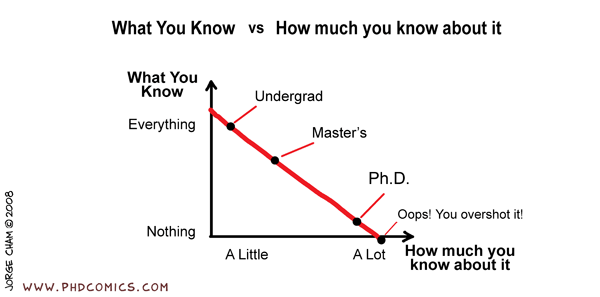
\includegraphics[width=0.7\linewidth]{Figures/comic.png}
\end{figure}

A common joke made about completing a PhD is that it teaches you a great deal about an insignificantly tiny slice of a field.
I would like to think I've come out a bit better than that (I know slightly less than a great deal about at least two tiny slices of chemistry), which I attribute almost entirely to my supervisor, Jonathan White.
I was lucky enough to stumble (literally, after a 21\textsuperscript{st} birthday the night before) into his group as a na\"ive Masters student, where I was immediately struck by the diversity of projects and people in the group.
From radiochemistry to photovoltaics, it seemed Jonathan could do anything.
I tried to imbibe as much of this attitude as I could during my Masters and PhD, sometimes ending up with a bit too much on my plate.
Nonetheless, thanks to Jonathan's wise counsel, I was able to tie almost all of the loose ends and disparate projects into this thesis.
I think this hunger for knowledge and eye for serendipity is one of the greatest gifts a supervisor could bestow on a PhD student, and for this I thank him profusely.

I also thank my PhD committee members, Brendan Abrahams and Uta Wille.
I genuinely looked forward to and enjoyed our annual progress meetings.
You both always provided such wonderful ideas and tangents for my projects, which I would never have otherwise thought of pursuing.
Along with Jonathan, you both helped to expose me to your respective areas of expertise, and I look forward to taking some of that knowledge with me to my first post-doc role.
Of course I shouldn't need to mention the incredible support and kindness you showed me.
I suppose I'm lucky I never had to, but I wouldn't have hesitated to come to either of your with any issues.
So thank you both, I couldn't have done it without you.

I owe a great deal to Colin Skene, for all the hands-on training throughout my Masters.
He also taught me the value of scientific rigour and detailed record-keeping, which I've tried to maintain as best as I can.

To all the members of the White group, past and present, thank you.
It's been an honour to work alongside such accomplished scientists, and your friendship is truly appreciated.
A special mention for the honorary White Walkers, Michael Ricca and Tze Cin Owyong, who have been a perpetual source of good times.
I will greatly miss our nights at Naughton's.

I thank all the wonderful friends I've made in the School of Chemistry.
Pre-COVID Friday Frothies were a monthly highlight, and the kick-ons to whichever watering hole happened to be open always reassured me that I had fallen into an excellent cohort.
On that note, I should also thank all the bar staff at Naughton's, The Clyde, Bobbie Peel's, and The Castle for so tactfully dealing with us rowdy chemists, and our heated late-night discussions over DFT functionals.

Thank you to my family, for 27 years of love and support, and for instilling in me the value of education.

Finally, I thank my loving partner, Alex Cummaudo.
You've taught me so much throughout our time together, not just about \LaTeX{}, but about persistence, compromise, and the value of family.
I'm so proud that I got to complete my PhD side by side with you, and I look forward to many more years with you and Pickles 
\includegraphics[width=1em]{Figures/pickles.png}.
}
\clearpage  % End of the Acknowledgements
%% ----------------------------------------------------------------

\pagestyle{fancy}  %The page style headers have been "empty" all this time, now use the "fancy" headers as defined before to bring them back

%% ----------------------------------------------------------------
%\lhead{\emph{Contents}}  % Set the left side page header to "Contents"
\tableofcontents  % Write out the Table of Contents

%% ----------------------------------------------------------------
%\lhead{\emph{List of Figures}}  % Set the left side page header to "List if Figures"
\listoffigures  % Write out the List of Figures

%% ----------------------------------------------------------------
%\lhead{\emph{List of Tables}}  % Set the left side page header to "List of Tables"
\listoftables  % Write out the List of Tables

%% ----------------------------------------------------------------
\setstretch{1.5}  % Set the line spacing to 1.5, this makes the following tables easier to read
\clearpage  % Start a new page


%\lhead{\emph{List of Compounds}} 
\listofcompounds{lll}  % Include a list of Abbreviations (a table of two columns)
{
\textbf{\#} & \textbf{Compound code} & \textbf{Structure} \\
\cmpdrow{ebs}{ebs.eps} \\
\refcmpd{ebs}\textbf{R} & \texttt{ebs.4R} & \vspace{0.4cm}\parbox[l]{4cm}{\centering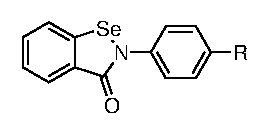
\includegraphics[scale=0.6]{Figures/loc/ebs_r.eps}} \\
\cmpdrow{ebs.thio}{ebs_thio.eps} \\
\cmpdrow{ebs.bn}{ebs_bn.eps} \\
\cmpdrow{ebs.h}{ebs_h.eps} \\
\cmpdrow{ebs.h-thio}{ebs_h-thio.eps} \\
\cmpdrow{amide}{amide.eps} \\
\cmpdrow{amide.bn}{amide_bn.eps} \\
\cmpdrow{amide.h}{amide_h.eps} \\
\cmpdrow{tetracycle}{tetracycle.eps} \\
\cmpdrow{py.pyrrol}{py_pyrrol.eps} \\
\cmpdrow{py.morph}{py_morph.eps} \\
\cmpdrow{diselenide}{diselenide.eps} \\
\cmpdrow{dichloride}{dichloride.eps} \\
\cmpdrow{dimethylcyclohexanone-oxime-dnp}{dimethylcyclohexanone-oxime-dnp.eps} \\
\cmpdrow{cyclohexanone-oxime-dnp}{cyclohexanone-oxime-dnp.eps} \\
\cmpdrow{acetone-oxime-dnp}{acetone-oxime-dnp.eps} \\
\cmpdrow{cyclohexanone-oxime-2np}{cyclohexanone-oxime-2np.eps} \\
\cmpdrow{cyclohexanone-oxime-2n.5nme2p}{cyclohexanone-oxime-2n_5nme2p.eps} \\
\cmpdrow{cyclohexanone-oxime-2n.5mp}{cyclohexanone-oxime-2n_5mp.eps} \\
\cmpdrow{m2pb}{m2pb.eps} \\
\cmpdrow{ebs-rhs-2py}{ebs-rhs-2py.eps} \\
%\cmpdrow{ebs-ebs-2py}{ebs-ebs-2py.eps} \\
\cmpdrow{ebs-nitroamide-2py}{ebs-nitroamide-2py.eps} \\
\cmpdrow{ebs-nitroaniline}{ebs-nitroaniline.eps} \\
\cmpdrow{rhs-bromo-2py}{rhs-bromo-2py.eps} \\
\cmpdrow{bromodiamine}{bromodiamine.eps} \\
\cmpdrow{2py-carboximidate}{2py-carboximidate.eps} \\
\cmpdrow{rhs-bromo-ph}{rhs-bromo-ph.eps} \\
\cmpdrow{rhs-bromo-ph.pmb}{rhs-bromo-ph_pmb.eps} \\
\cmpdrow{ebs-rhs-ph}{ebs-rhs-ph.eps} \\
\cmpdrow{ebs-rhs-ph.thio-pmb}{ebs-rhs-ph_thio-pmb.eps} \\
\cmpdrow{ebs-rhs-2py-diselenide}{ebs-rhs-2py-diselenide.eps} \\
\cmpdrow{rhs-nitro-amide}{rhs-nitro-amide.eps} \\
\cmpdrow{rhs-nitro}{rhs-nitro.eps} \\
\cmpdrow{rhs-amine}{rhs-amine.eps} \\
}

\begin{comment}
%\lhead{\emph{Abbreviations}}  % Set the left side page header to "Abbreviations"
\listofsymbols{ll}  % Include a list of Abbreviations (a table of two columns)
{
% \textbf{Acronym} & \textbf{W}hat (it) \textbf{S}tands \textbf{F}or \\
\textbf{LAH} & \textbf{L}ist \textbf{A}bbreviations \textbf{H}ere \\

}

%% ----------------------------------------------------------------
\clearpage  % Start a new page
%\lhead{\emph{Constants}}  % Set the left side page header to "Physical Constants"
\listofconstants{lrcl}  % Include a list of Physical Constants (a four column table)
{
% Constant Name & Symbol & = & Constant Value (with units) \\
Speed of Light & $c$ & $=$ & $2.997\ 924\ 58\times10^{8}\ \mbox{ms}^{-\mbox{s}}$ (exact)\\

}

%% ----------------------------------------------------------------
\clearpage  %Start a new page
%\lhead{\emph{Symbols}}  % Set the left side page header to "Symbols"
\listofnomenclature{lll}  % Include a list of Symbols (a three column table)
{
% symbol & name & unit \\
$\sigma$ & chemical shielding\\
$\sigma$ & estimated standard deviation\\
}
\end{comment}
%% ----------------------------------------------------------------
% End of the pre-able, contents and lists of things
\clearpage

%% ----------------------------------------------------------------
\mainmatter	  % Begin normal, numeric (1,2,3...) page numbering
\pagestyle{fancy}  % Return the page headers back to the "fancy" style

% Include the chapters of the thesis, as separate files
% Just uncomment the lines as you write the chapters

\part{Background}

\begin{refsection}
\chapter{Introduction}\label{ch:intro}

The importance of non-bonding interactions in our world simply cannot be overstated.
While we may think of the more familiar covalent and ionic bonds as the core of chemistry, more often than not it is non-bonding interactions that dictate the nature of substances, from bulk properties such as tensile strength, to microscopic phenomena like protein-ligand interactions.

At a fundamental level, all non-bonding interactions (indeed, conventional bonding too) are attributable to the electrostatic force.
However, it is more convenient to broadly categorise interactions based on strength and structural motifs that are common to each class.
Such classes include dispersion forces, dipole-dipole interactions, and hydrogen bonding (H-bonding).
In the 19th century, it became apparent that these classes paint an incomplete picture of intermolecular bonding.
As part of their investigation into solvent effects on the colour of iodine solutions in 1949, Bensei and Hildebrand invoked the concept of ``charge-transfer'' complexes to explain the association of molecular iodine with nucleophilic solvent molecules.\autocite{Benesi1949}
Although the electrophilic nature of molecular halogens was already well appreciated with respect to reactivity, this appears to be the first acknowledgement that this understanding could be applied to ground state complexes.
In support of this, Hassel and Hvoslef elucidated the structure of a 1:1 complex of molecular bromine and 1,4-dioxane in 1954, and observed an unusually strong interaction between the two molecules.\autocite{Hassel1954}
The crystal was comprised of long chains of monomers (\cref{fig:hassel-xray}), exhibiting a very short \ce{O \cdots Br} contact (2.71~\AA, the sum of the van der Waals (VDW) radii is 3.37~\AA), and a slightly lengthened \ce{Br-Br} bond (2.31~\AA\ vs 2.28~\AA\ in gaseous bromine).

\begin{figure}[ht]
  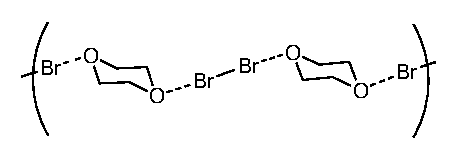
\includegraphics[width=0.6\columnwidth]{Figures/hassel-xray.eps}
  \caption[Bromine-dioxane complex.]{Long chains of molecular bromine and 1,4-dioxane, observed by Hassel and Hvoslef.}\label{fig:hassel-xray}
\end{figure}

In the subsequent years, a wide variety of names and labels were applied to the ``charge-transfer'' phenomenon, including ``lock and key'', ``donor-acceptor'', and ``filling of anti-bonding orbitals'', as summarised in Bent's excellent 1968 review\autocite{Bent1968}.
The term ``halogen bonding'' (X-bonding) only gained widespread acceptance in 1983 after the review of Dumas, Gomel, and Guerin.\autocite{Dumas1983}
The term deliberately evokes similarity to the better known concept of hydrogen bonding, as the two phenomena are of comparable strength and, importantly, directionality.
In 1998 Anthony C. Legon again used the term to describe the attractive interaction between halogens and Lewis bases in pre-reactive complexes, harking back to the original understanding of electrophilic halogens as a primarily reactive phenomenon.\autocite{Legon1998,Legon1999}
In the following years, the potential of X-bonding was more fully recognised, with applications in supramolecular chemistry and self-assembly\autocite{Corradi2000,Metrangolo2008,Priimagi2013}, catalysis and bond activation\autocite{Walter2011,Soloshonok2017,Takagi2017}, and molecular sensing and recognition\autocite{Cornes2017,VargasJentzsch2013,Borissov2017}.

From X-bonding grew the related concepts of chalcogen (Ch-), pnictogen (Pn-), and tetrel bonding (T-bonding), as the electrophilic nature of these elements was discovered.\autocite{Murray2007}
Similar applications have also been found for these classes of non-covalent interactions, Ch-bonding in particular.\autocite{Fanfrlik2014,Garrett2016,Ho2016,Wonner2017,Mitchell2017,Benz2017,Biot2018,Ho2017}

\section{Chalcogen Bonding}
Ch-bonding is the attractive interaction between a Lewis base and a chalcogen atom bearing an electron withdrawing substituent (\cref{fig:ch-bonding-intro}).
The terminology of Ch-bonding partners is perhaps counter-intuitive, as donors and acceptors are named by analogy with H-bonded equivalents.
Note this is contrary to the formal flow of electron density; Ch-bond \emph{donors} bear vacant \emph{acceptor} orbitals, while Ch-bond \emph{acceptors} are \emph{donors} of electron density.
For the purposes of this thesis, ``donor'' will refer to the Lewis acidic chalcogen species.

\begin{figure}
    \centering
    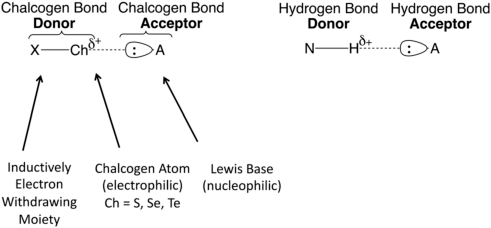
\includegraphics[width=0.8\linewidth]{Figures/ch-bonding.pdf}
    \caption{Chalcogen bonding model, and similarity to H-bonding.}\label{fig:ch-bonding-intro}
\end{figure}

\subsection{Mechanisms}
As was discussed in the previous section, all intermolecular (and indeed \emph{intra}mole\-cular) forces are manifestations of the electromagnetic force.
Nonetheless, it is more convenient to categorise energetic contributions to any given interaction as orbital, electrostatic, or dispersion mediated, as there are marked differences in strength and directionality between them.
Historically, X- and Ch-bond interactions were understood to be primarily due to orbital overlap and resulting charge transfer.
Evidence for this included the lengthening of the \ce{X-X} bond corresponding to increased occupation of the $\sigma^{\star}$(\ce{X-X}) orbital due to the incoming lone pair (this was observed in Hassel and Hvoslef's original work\autocite{Hassel1954}).
Characteristic charge transfer bands are also observed in the UV-vis spectra of halogen solutions.\autocite{Blackstock1987}

Such evidence of orbital contributions is not, however, common to all systems displaying X- or Ch-bond interactions.
The iodoperfluoroalkanes and arenes studied by \citeauthor{Yan2014} show no charge transfer bands in UV-vis spectra, yet are exceptionally strong X-bond donors.\autocite{Yan2014}
Murray and Politzer have advocated for an alternative, primarily electrostatic explanation of X- and Ch-bond interactions.\autocite{Murray2008,Murray2009}
They propose that a positively charged $ \sigma $-hole is generated along the extension of a $ \sigma $ bond to an electron withdrawing substituent, due to polarisation of the electron cloud.
This also adequately explains the strength and directionality of these interactions.
An interpretation which has not attracted as much attention is that of dispersion forces.

While the varying contributions from each of these factors can be dissected computationally via perturbation methods, experimental evidence is surprisingly sparse.
Pascoe, Ling and Cockroft, however, devised an elegant experiment to quantitatively determine energetic contributions.\autocite{Pascoe2017}
\textsuperscript{19}F-NMR was used to determine the relative populations of two conformers of a ``molecular balance'', one bearing a Ch-bond interaction, one not (\cref{fig:cockroft-balances}).
Interaction energies were thus derived, and found to be more or less invariant with respect to the solvent.
This appeared to rule out electrostatic contributions, as solvent dipole moment and bulk polarisability would otherwise have a large effect on the position of the equilibrium.
These results also suggest that dispersion plays only a minor role, for similar reasons.

\begin{figure}
    \centering
    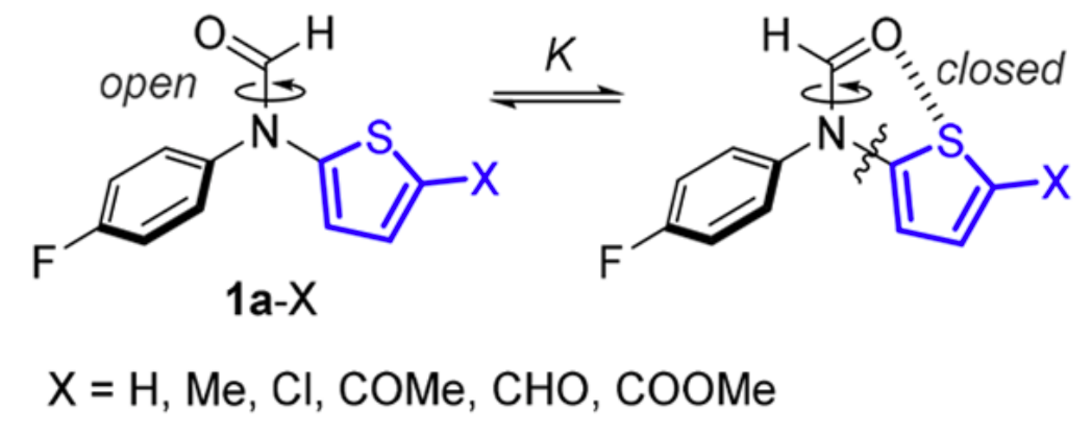
\includegraphics[width=0.6\linewidth]{Figures/cockroft-balances.pdf}
    \caption[``Molecular balances'' for the measurement of Ch-bond energies.]{``Molecular balances'' designed by \citeauthor{Pascoe2017} for the measurement of Ch-bond energies.\autocite{Pascoe2017}}\label{fig:cockroft-balances}
\end{figure}

In the same study, DFT was used to further probe the dispersion contribution.
Free energies were calculated using functionals which both did, and did not include dispersion corrections, and the values compared to the experimental results.
The non-dispersion corrected B3LYP functional gave superior correlation with experiment than did either M06-2X and $ \omega $B97X-D, both of which include dispersion (either via parametrization or as an empirical correction).
This provided additional evidence that, in the systems studied, the major contributor to the interaction is orbital overlap and charge transfer.

Although current evidence points towards these interactions being primarily orbital related, the electrostatic ``$ \sigma $-hole'' terminology of Politzer and Murray has stuck, and the term is now used to encompass the whole gamut of X-, Ch-, Pn- (pnictogen), and T- (tetrel) bonding interactions.

\section{Applications of Ch-Bonding}
Ch-bonding, and by extension, all $ \sigma $-hole interactions can theoretically be applied to any formal Lewis acid-base system.
They are especially attractive as a hydro\emph{phobic} complement to H-bonding interactions, which are generally considered to be hydro\emph{philic}.
The following are brief summaries of existing applications in the literature.

\subsection{Materials}
The major applications of $ \sigma $-hole interactions have so far been in the realm of crystal engineering.
Early work by \citeauthor{Corradi2000} showed that halogen bonding was able to outcompete H-bonding in the formation of supramolecular architectures.\autocite{Corradi2000}
A review by \citeauthor{Metrangolo2008} summarised the forms that are accessible using X-bonding to direct crystal growth.\autocite{Metrangolo2008}
1D, 2D, and 3D architectures are able to be generated using appropriate X-bond donors, and these show potential in the design of liquid crystals, organic semiconductors and paramagnetic materials (\cref{fig:iodotempo-chains})
A more recent review by the same group described applications in anion transport, and luminescent and photo-responsive crystals.\autocite{Priimagi2013}
The group of Stefan Matile has further explored anion transport, and has published a review comparing X-bonding with other hydrophobic interactions such as anion-$ \pi $ and anion-macrodipole interactions (\cref{fig:matile-anion-binder}).\autocite{VargasJentzsch2013}

\begin{figure}
    \centering
    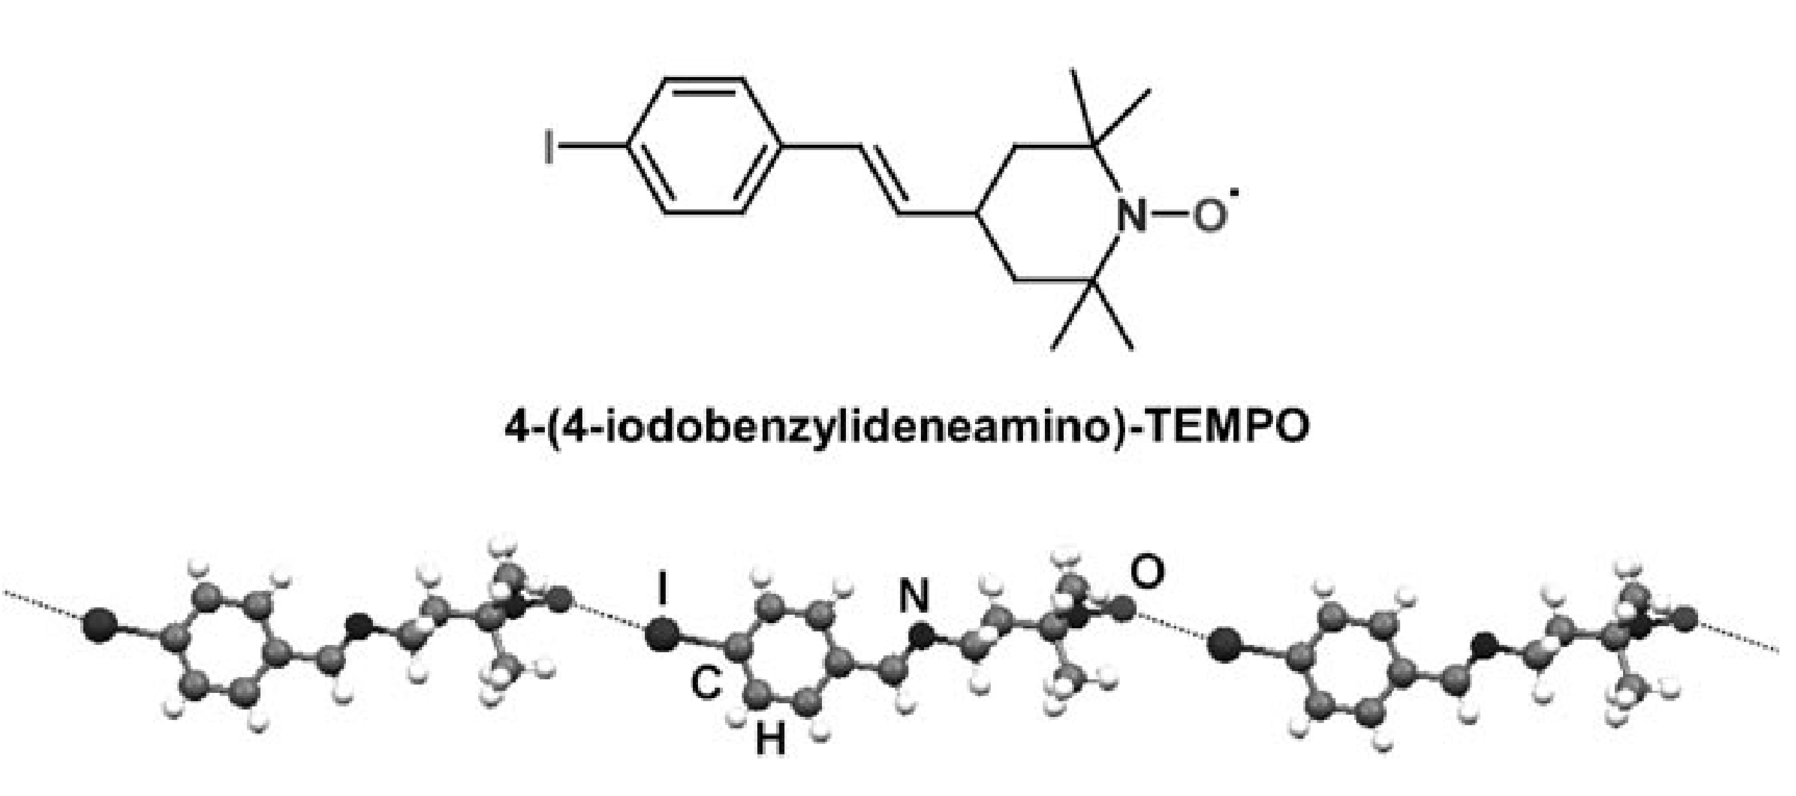
\includegraphics[width=0.6\linewidth]{Figures/iodotempo-chains.pdf}
    \caption[One-dimensional chains of 4-(4-iodobenzylidene)-TEMPO structured by X-bonds.]{One-dimensional chains of 4-(4-iodobenzylidene)-TEMPO structured by X-bonds.\autocite{Metrangolo2008}}\label{fig:iodotempo-chains}
\end{figure}

\begin{figure}
    \centering
    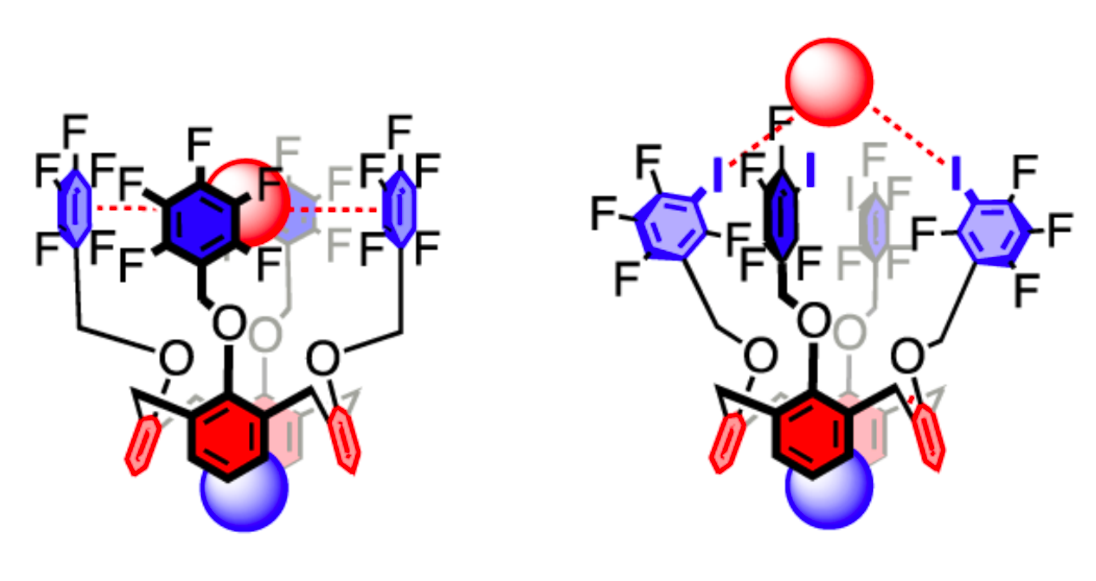
\includegraphics[width=0.4\linewidth]{Figures/matile-anion-binder.pdf}
    \caption[Anion binding through anion-$ \pi $ interactions and X-bonding.]{Anion binding through anion-$ \pi $ interactions and X-bonding.\autocite{VargasJentzsch2013} The red spheres represent anions and the blue spheres represent cations.}\label{fig:matile-anion-binder}
\end{figure}

Ch-bonding, too, has been investigated with respect to materials chemistry.
\citeauthor{Fanfrlik2014} demonstrated the importance of Ch-bonding on the crystal packing of thiaboranes.\autocite{Fanfrlik2014}
They found that the sulfur-based $ \sigma $-hole was sufficiently strong to interact with the weakly basic $ \pi $ electrons of a phenyl group, with contacts as short as 3.2~\AA\ being observed (\cref{fig:thiaborane-ch-bond}).

\begin{figure}
    \centering
    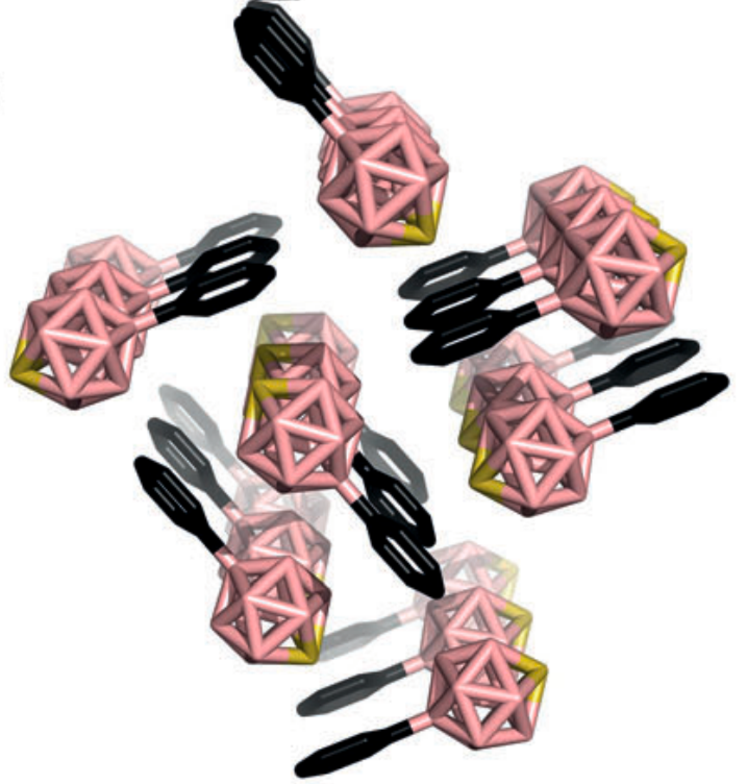
\includegraphics[width=0.45\linewidth]{Figures/thiaborane-ch-bond.pdf}
    \caption[Ch-bonding in thiaboranes.]{Ch-bonding in thiaboranes.\autocite{Fanfrlik2014}}\label{fig:thiaborane-ch-bond}
\end{figure}

In 2016, \citeauthor{Ho2016} published their work into tellurium-based Ch-bonding.\autocite{Ho2016}
Their scaffolds are based on an iso-tellurazole N-oxide, which reversibly forms macrocyclic structures that persist in both gas and solution phase (\cref{fig:te-pd-macrocycle}).
The macrocycles were found to coordinate \ce{Pd2+}.
This is particularly interesting, as the tellurium atoms are simultaneously behaving as a Lewis acid and base.
The authors point out that such soft macrocycles are quite rare, and their work could facilitate further studies of transition metals in a soft coordination environment.
They went on to investigate benzo-fused derivatives of iso-tellurazoles, as well as selenium analogues, which crystallised to form macromolecular pores and voids.\autocite{Ho2017}

\begin{figure}
    \centering
    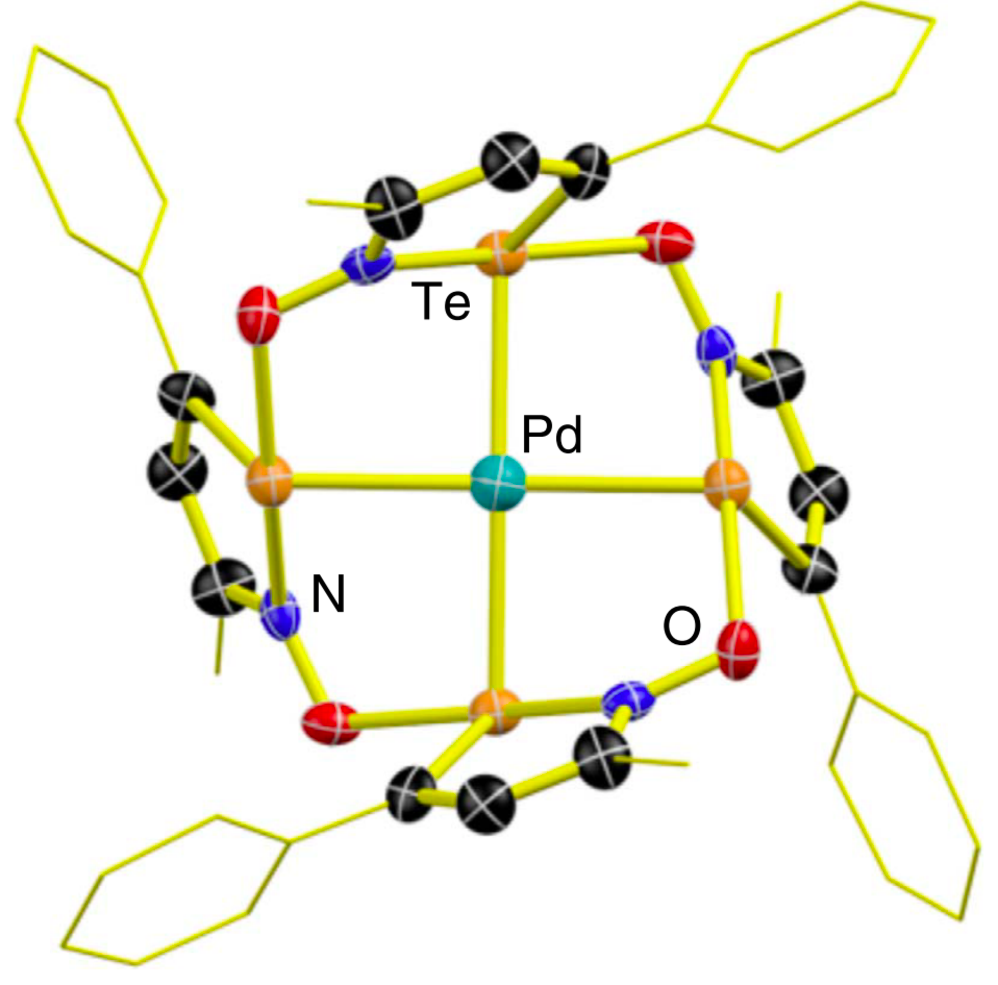
\includegraphics[width=0.4\linewidth]{Figures/te-pd-macrocycle.pdf}
    \caption[A tetrameric macrocycle held together by Ch-bonds.]{A tetrameric macrocycle held together by Ch-bonds.\autocite{Ho2016}}\label{fig:te-pd-macrocycle}
\end{figure}

The Taylor group has been active in the development of X- and Ch-bonding molecular sensors.
Early work demonstrated that X-bonding tridentate ligands (reminiscent of enterobactin) showed moderate selectivity for \ce{Cl-}.\autocite{Dimitrijevic2010}
They later developed bidentate Ch-bonding ligands which exhibited a tenfold increase in association constant with respect to chloride (\cref{fig:taylor-cl-binder}).\autocite{Garrett2015a,Garrett2016}

\begin{figure}
    \centering
    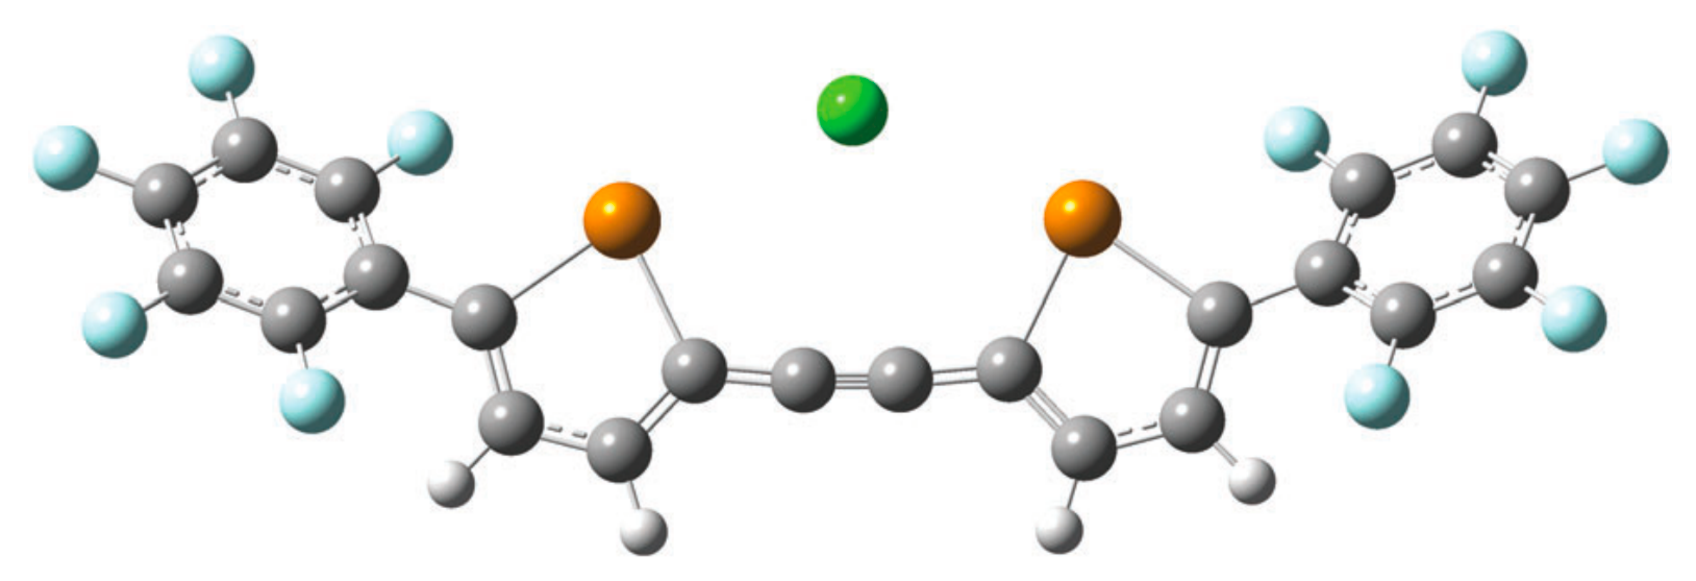
\includegraphics[width=0.6\linewidth]{Figures/taylor-cl-binder.pdf}
    \caption[A bidentate Ch-bonding anion binder.]{A bidentate Ch-bonding anion binder.\autocite{Garrett2016}}\label{fig:taylor-cl-binder}
\end{figure}

Similar results have been achieved by the Beer group, who have developed X-bonding sensors for the perrhenate anion.\autocite{Cornes2017}
These sensors are based on functionalised cyclodextrins, and are even more sensitive than the corresponding H-bonding analogues.
The group has also use iodotriazole scaffolds to chelate anions.\autocite{Borissov2017}
Incorporation of a chiral binaphthol moiety was shown to differentiate between enantiomers of chiral anions.

The role of selenium-based Ch-bonding on the crystal structure and mechanism of action of the drug ebselen was demonstrated by \citeauthor{Thomas2015}.\autocite{Thomas2015}
Ch-bonding between the selenium atom and carbonyl oxygen directs the crystal packing of this compound, and leads to the formation of one-dimensional chains of molecules (\cref{fig:ebs-packing}).
Interestingly, the Lewis acidity of the $ \sigma $-hole was invoked as an explanation of the antioxidant properties of the drug, as it can directly coordinate reactive oxygen species through a Ch-bond.
It can also form a covalent complex with glutathione (GSH) through the thiol functionality, thus mimicking glutathione peroxidase, which is the origin of its catalytic activity.\autocite{Azad2014}

\begin{figure}
    \centering
    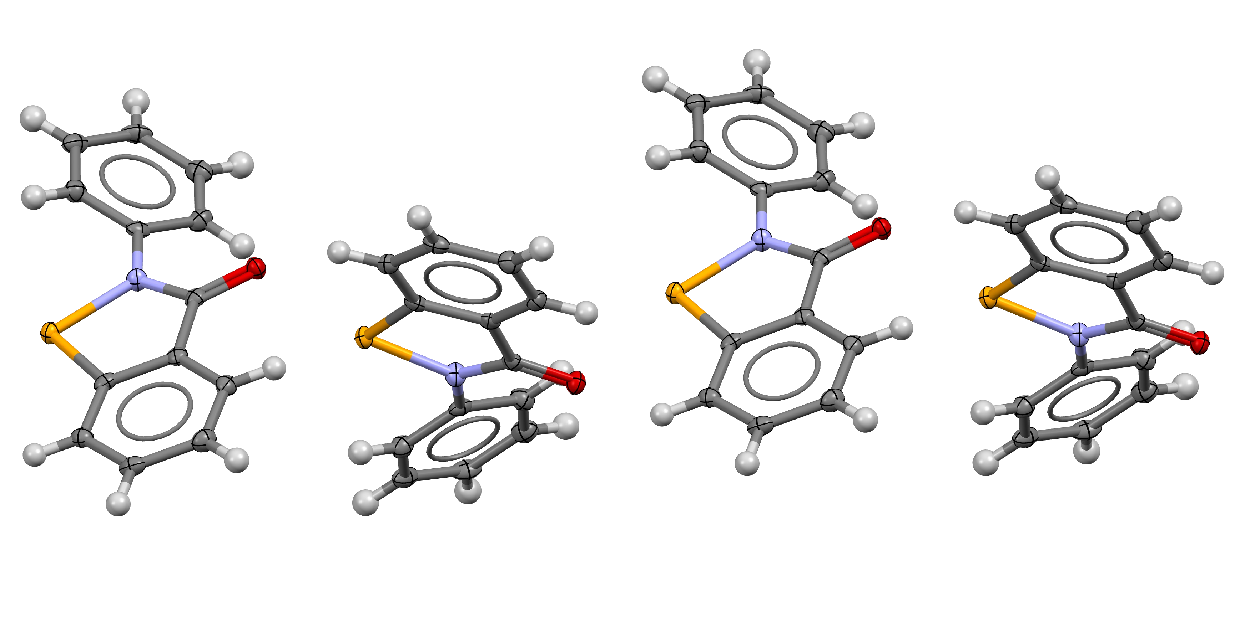
\includegraphics[width=0.7\linewidth]{Figures/ebs-packing.pdf}
    \caption{One dimensional chains formed in the crystal packing of ebselen.}\label{fig:ebs-packing}
\end{figure}

\subsection{Catalysis and bond activation}
In 2008, halogen bonding was first applied to a Hantzsch ester reduction of a quinoline derivative.\autocite{Bruckmann2008}
This reaction is well characterised and understood, and has been catalysed with a variety of Br\o nsted and Lewis acids.
The X-bond donors chosen were perfluoroiodoalkanes, and high conversions were achieved with modest catalyst loadings of 10\%.

In 2011, a modified Ritter reaction was devised wherein benzhydryl bromide was activated by a dicationic imidazolium-based X-bond donor to give the carbocation intermediate, which was then captured by acetonitrile and then hydrolysed to afford the amide product.\autocite{Walter2011}
This pioneering work was limited by the necessity of stoichiometric amounts of the X-bond donor, as it is consumed in the course of the reaction.

A similar alkylation of 1-chloroisochroman was achieved by the same group using a neutral perfluoroiodoarene X-bond donor in catalytic quantities.\autocite{Kniep2013}
The proposed mechanism is similar to the thiourea-catalysed reaction of \citeauthor{Reisman2008}\autocite{Reisman2008}, which has shown promise in asymmetric induction.
The authors noted issues with solubility of the perfluoroiodoarene catalysts, which is expected of such highly fluorinated compounds.

The reduction of quinoline was successfully catalysed by a dithiophene system by \citeauthor{Benz2017} in 2017\autocite{Benz2017}, and then again by the same group with a benzodiselenazole (\cref{fig:quinoline-redn}).\autocite{Benz2017a}
With the increased selectivity and strength of the Se-based Ch-bonding catalyst compared to the X-bonding perfluoroiodoalkane, the authors were able to reduce the catalyst loading to 1\%.

\begin{figure}
    \centering
    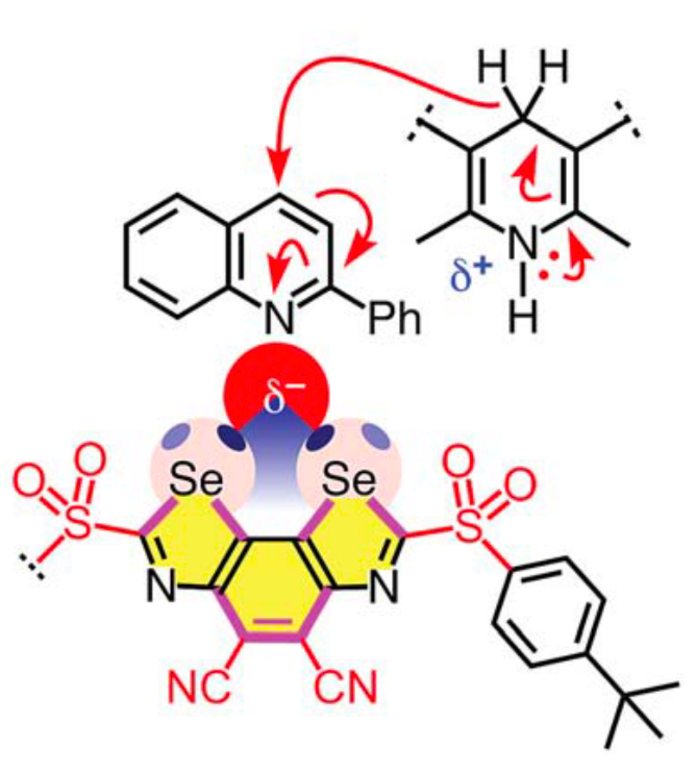
\includegraphics[width=0.4\linewidth]{Figures/quinoline-redn.pdf}
    \caption[Proposed mechanism for the catalytic reduction of quinoline by a Ch-bonding catalyst.]{Proposed mechanism for the catalytic reduction of quinoline by a Ch-bonding catalyst.\autocite{Benz2017}}\label{fig:quinoline-redn}
\end{figure}

\citeauthor{Wonner2017} developed a selenated bis-benzimidazolium Ch-bonding catalyst for the alkylation of 1-chloroisochroman, and solvolysis of benzhydryl bromide.\autocite{Wonner2017,Wonner2017a}
Although the best results were observed with the dicationic catalysts, conversion was also achieved with a neutral bis-benzimidazole catalyst, providing further evidence that the catalytic Lewis-acid site is indeed the $ \sigma $-hole.
For a given row in the periodic table (i.e.\ comparing a Se-based donor to a Br-based donor), Ch-bonding appeared to give superior results to X-bonding, as measured by \% yield.

An unusual manifestation of X-bonding is in the self-disproportionation of enantiomers, as reported by \citeauthor{Soloshonok2017}.\autocite{Soloshonok2017}
They observed spontaneous enrichment of one enantiomer of mebroqualone (\cref{fig:mebroqualone}) upon chromatography using an achiral solid phase, which they attributed to the formation of diastereomeric X-bonded oligomers.
This phenomenon has been observed in compounds capable of interacting through H-bonding or strong dipole-dipole interactions.\autocite{Cundy1983}

\begin{figure}
    \centering
    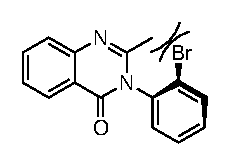
\includegraphics[scale=0.8]{Figures/mebroqualone.eps}
    \caption[The structure of mebroqualone.]{The structure of mebroqualone. Rotation is hindered about the biaryl bond, allowing the isolation of two atropisomers.}\label{fig:mebroqualone}
\end{figure}

\subsection{Biological systems}

\subsubsection{Proteins}
While we usually think of the tertiary structure of proteins as being dominated by H-bonding and hydrophobic effects, there is increasing evidence that Ch-bonding plays an important role as well.
This is not unexpected, as sulfur, a component of both cysteine and methionine, is known to form Ch-bonds in small molecules.
In the early days of Ch-bonding interactions (2001, before the name had come into common use) \citeauthor{Iwaoka2001} published an analysis of 604 protein structures in the Protein Data Bank (PDB).\autocite{Iwaoka2001}

A remarkable number of close contacts (sum of Van der Waals radii plus 0.5~\AA) between sulfur and Lewis basic (LB) atoms were identified in the structures, with 33\% of cysteine residues and 22\% of methionine residues showing a close contact.
Furthermore, the geometric parameters of these contacts were studied, with more than half of all contacts having a \ce{S-S-LB} (LB = O, N) of 150--180\degree.
The observed contacts were ascribed to a $ \pi $(\ce{C=O}) $ \rightarrow \sigma^{\star} $(\ce{S-S}) interaction, in contrast to the n(LB)$ \rightarrow \sigma^{\star} $(\ce{S-X}) interaction which dominates in small molecules, where X is an electronegative atom.
Also contrary to the case of small molecules, the authors suggested that the orbital component of the interaction is small, though important for establishing the directionality of the interaction.
Dispersion appears to be the major stabilising force, as optimization using a non-dispersion corrected level of theory gave unrealistically large distances between the two interacting groups.

The differences between Ch-bonding in proteins and small molecules is likely due to variation in orbital energies in the functional groups which are found in each class.
While small molecule Ch-bond donors are characterised by easily accessible, low energy $ \sigma^{\star} $(\ce{Ch-X}) orbitals, these are simply not found in proteins.
Instead, donors are characterised by $ \sigma^{\star} $(\ce{S-S}) or $ \sigma^{\star} $(\ce{S-C}) orbitals, which are much higher in energy and less accessible to acceptors.
Ch-bond acceptors, too, are markedly different between small molecules and proteins.
In general, the HOMO of a system (the most Lewis basic site) is dominated by lone pairs.
This is observed in most small molecules, as they form Ch-bonds through these lone pairs.
However, the amide bond, which is ubiquitous in proteins, shows an unusual inversion in orbital energies.
The $ \pi $(\ce{C=O}) orbital is elevated with respect to the lone pair according to MP2 calculations, making it the more basic site.
Structural data supports this assertion, as the Ch-bond donor usually approaches the top of the C=O bond in proteins, rather than the usual approach towards the oxygen lone pair (\cref{fig:amide-diselenide-ch-bond}).\autocite{Iwaoka2012}

\begin{figure}
    \centering
    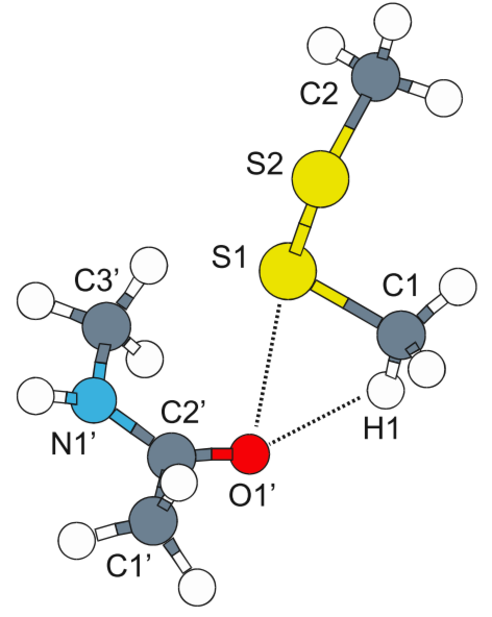
\includegraphics[width=0.4\linewidth]{Figures/amide-diselenide-ch-bond.pdf}
    \caption{Directional preference for Ch-bonded interactions in proteins.}\label{fig:amide-diselenide-ch-bond}
\end{figure}

It is worth noting that selenium is also found in proteins as selenocysteine and selenomethionine.
This would be expected to be an even stronger Ch-bond donor.
However, selenoproteins are relatively few in number, precluding such extensive statistical analysis.\autocite{Iwaoka2015}
They are only mentioned here for the sake of completeness.

Intramolecular interactions are just one instance of Ch-bonding in biological systems.
Proteins often interact with ligands or substrates through H-bonds, so it is reasonable to propose that Ch-bonding could be applied in this field as well.
Indeed, a protein-ligand Ch- and X-bonding interaction was used to target the gatekeeper methionine (MET146) residue of c-Jun N-terminal kinase 3 (JNK3) in a model study by \citeauthor{Lange2015}.\autocite{Lange2015}
In this work, a protein$ \rightarrow $ligand Ch-bond was used to stabilise the interaction.
Inhibition of a cysteine protease using a variety of sulfur-containing heterocyclic ligands was also investigated.\autocite{Giroud2017}
These ligands formed ligand$ \rightarrow $protein Ch-bonds, complementary to the the work by Lange.
Non-conventional protein-ligand interactions are summarised in a comprehensive review by \citeauthor{Beno2015}.\autocite{Beno2015}

\subsubsection{Nucleic acids}
Nucleic acids represent another application of Ch-bonding in biology.
In addition to their crucial role in the storage of genetic information, they have also been investigated as a structural material in nanotechnology.
The ubiquity of H-bonds in nucleic acid complexes suggests that $ \sigma $-hole interactions may also be used to direct formation of these complexes.
X-bonding was indeed able to be used to direct formation of a Holliday junction between two DNA strands (\cref{fig:holliday-junction}).\autocite{Voth2007}
Holliday junctions are branched nucleic acid structures that appear in many biological processes including recombination and double-strand break repair.
They are also useful as building blocks for DNA nanotechnology, where their self assembly and predictable geometry are exploited.
The authors estimated that the X-bonding interaction (mediated through a bromo-substituent) was 2--5 kcal$\cdot$mol$^{-1}$ stronger than the corresponding H-bond.
A 2017 review identified a further 21 X-bonded nucleic acid structures.\autocite{Kolar2017}
X-bonding was in fact able to partially replace inter-strand H-bonding interaction in a DNA oligomer.\autocite{Parker2012}

\begin{figure}
    \centering
    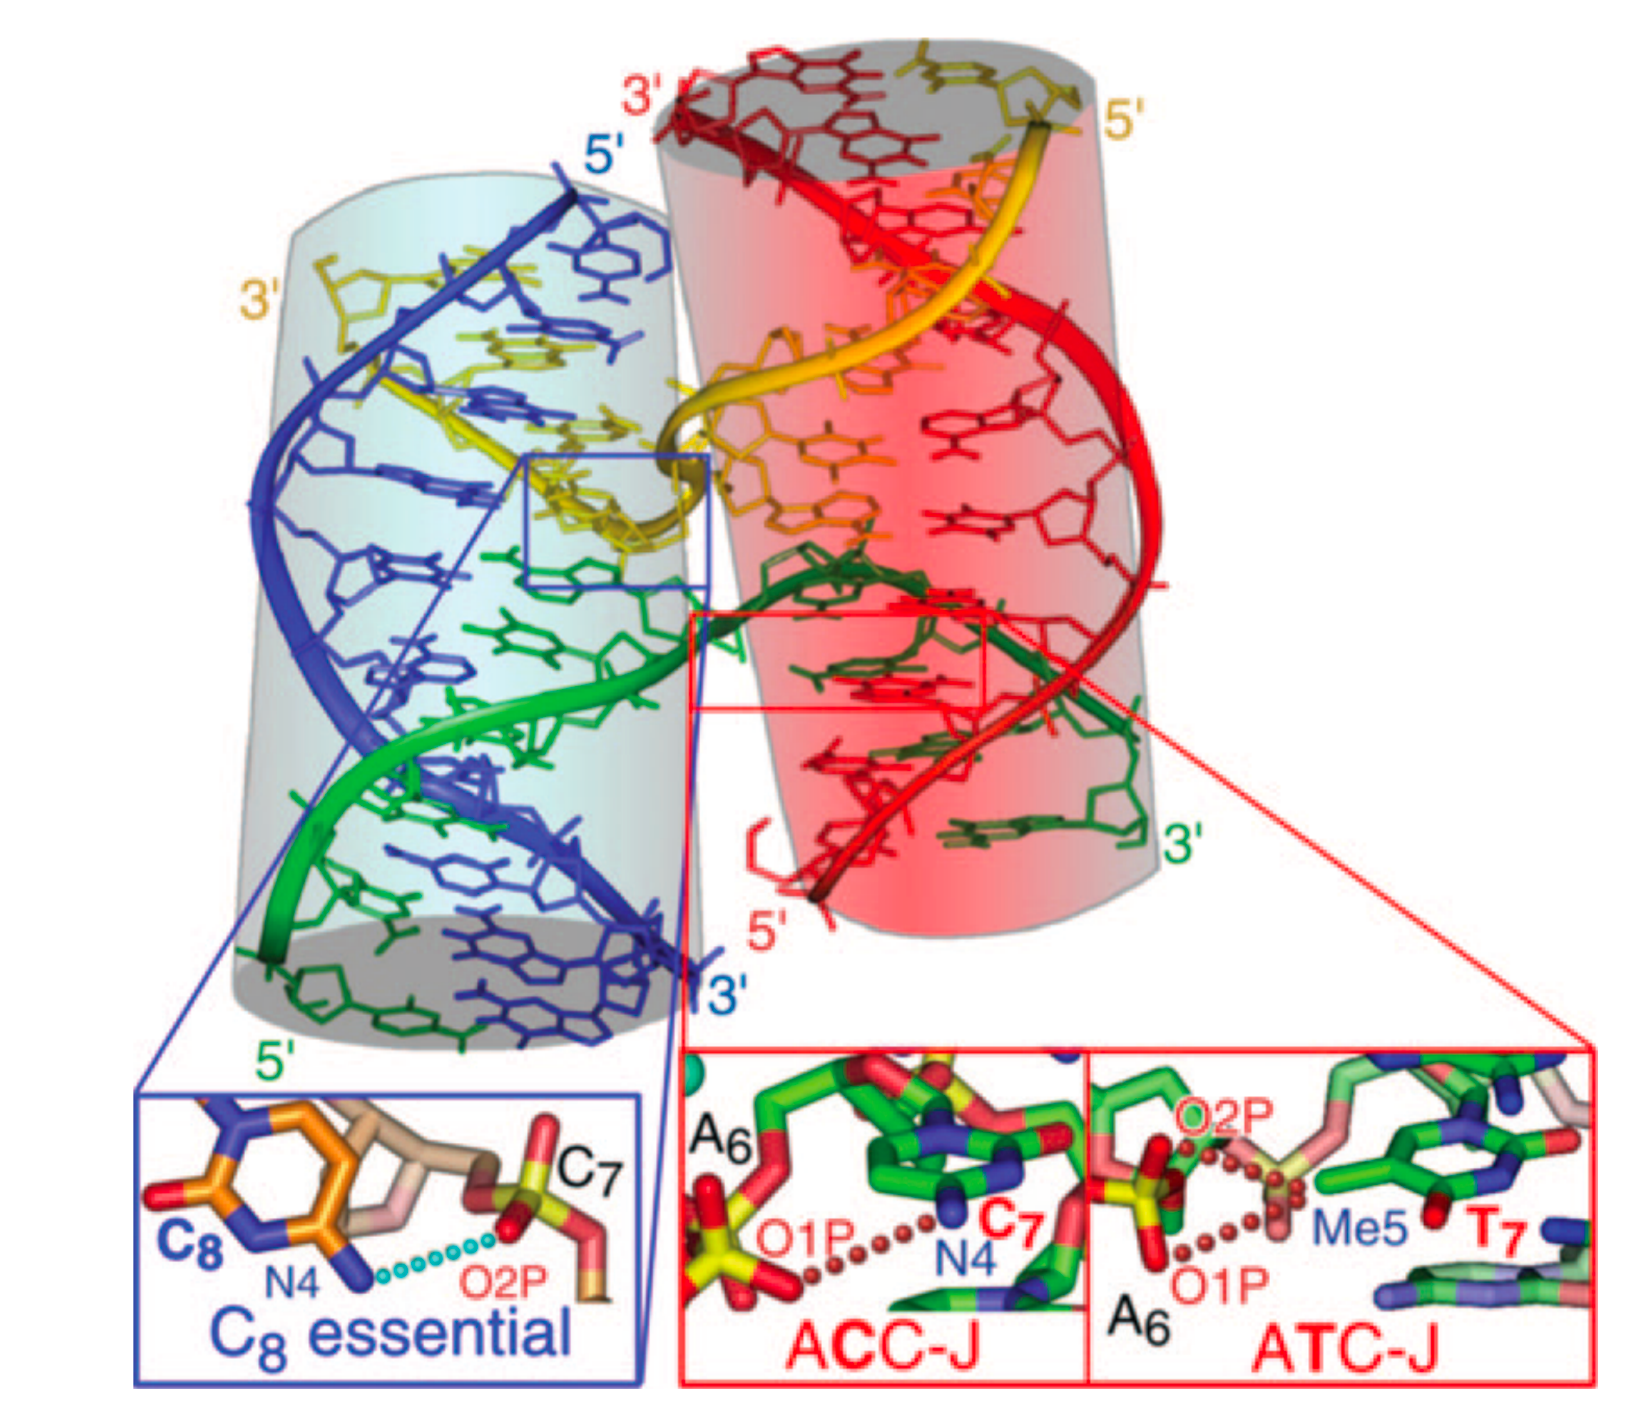
\includegraphics[width=0.6\linewidth]{Figures/holliday-junction.pdf}
    \caption[Holliday junction formed by X-bonding.]{Holliday junction formed by X-bonding.\autocite{Voth2007}}\label{fig:holliday-junction}
\end{figure}

Ch-bonding, too, has been investigated in the context of nucleic acids.
\Citeauthor{Sharma2020} recently investigated the possibility of forming Ch-bonded analogues of the canonical A:T/G:C base pairs in order to expand the genetic alphabet.\autocite{Sharma2020}
A G\textsubscript{\ce{SeF}}:C dimer was found to be more stable than the canonical G:C pair, where the \ce{SeF} subscript indicates that one of the H-bond donors on the guanine was replaced by a selenenyl fluoride.
\Citeauthor{Farrell2018} showed that introducing heavy chalcogens into nucleobases has profound impacts on their photochemistry, with implications for their use in photodynamic therapy.\autocite{Farrell2018}
The photophysics of selenonucleobases has been further explored, showing that they are uniquely photo-stable while efficiently populating and depopulating their excited states.\autocite{Mai2019,Peng2020,Fang2019,Uleany2020}
While none of these investigations specifically mentioned Ch-bonding, it is highly likely that it would come into play, which may provide a means of directing the activity of these photo-sensitisers.

\begin{figure}
    \centering
    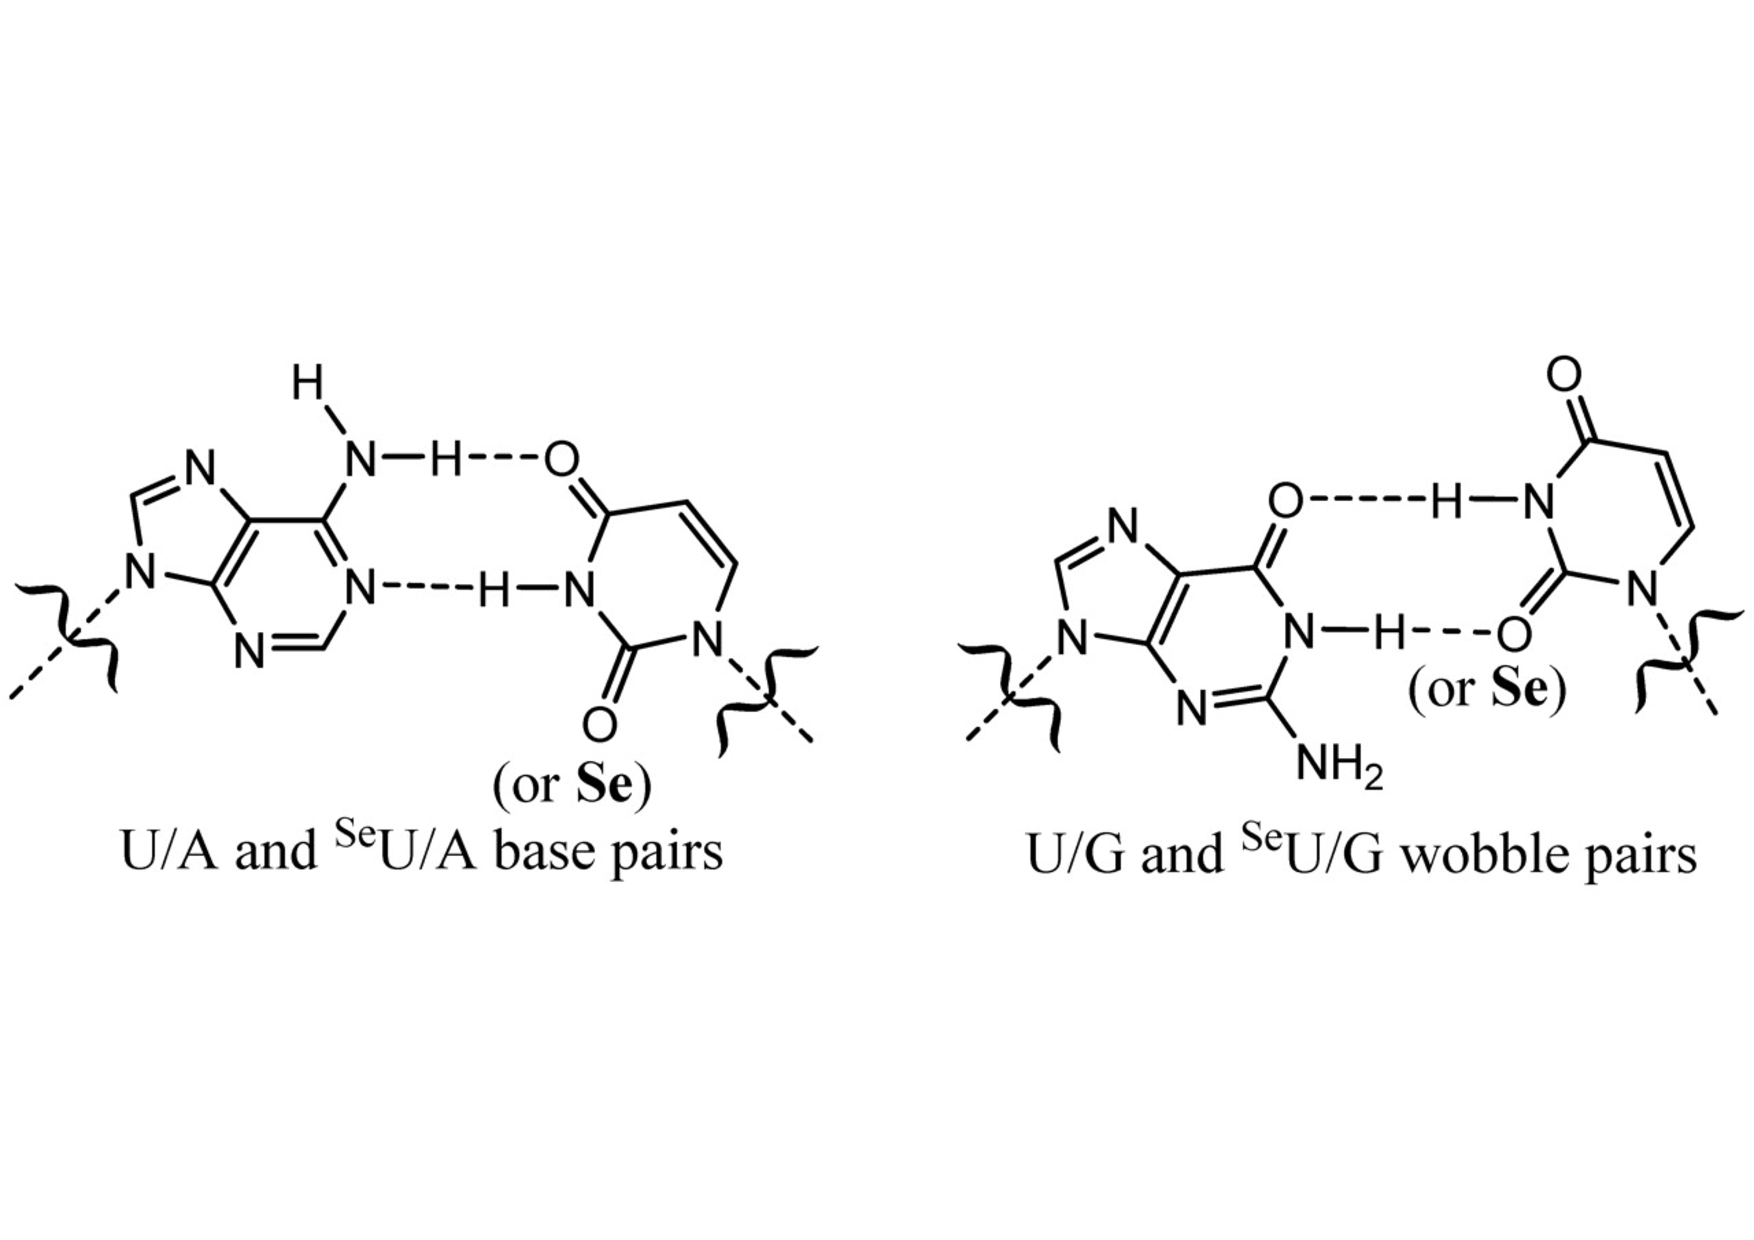
\includegraphics[width=0.6\linewidth]{Figures/wobble-bp.pdf}
    \caption[Canonical Watson-Crick U/A base pair, and the ``wobble'' U:G base pair in RNA.]{Canonical Watson-Crick U:A base pair, and the ``wobble'' U/G base pair in RNA.\@ The latter is disfavoured when an oxygen atom in uracil is substituted by selenium.}\label{fig:wobble-bp}
\end{figure}

Selenium has also been incorporated into nucleobases as a H-bond acceptor, in which it was shown that selenonucleobases can effectively discriminate against the formation of a so-called ``wobble'' base pair (U:G as opposed to U:A in RNA, or T:G/T:A in DNA, \cref{fig:wobble-bp}).\autocite{Hassan2010,Sun2012}
Another advantage of selenonucleobase incorporation is the ability to use the heavy selenium atom for MAD/SAD phasing of macromolecular crystal structures.\autocite{Salon2007}
This was also the motivation for a \citeyear{Conlon2019} study in which the selenium was incorporated into the phosphate backbone.\autocite{Conlon2019}
A major advantage of this approach is that the bulk of the selenium atom does not need to be accommodated in the interior of the double helix, so structural distortions are minimised.
To date, there have not been any drugs which target nucleic acids through Ch-bonding, which is an area we explore in \cref{ch:dna-binder}.

\section{Context of this work}
In this thesis, we examine some of the fundamental aspects of Ch-bonding in real-world systems, motivated by the end goal of developing a Ch-bonding DNA binder.
We identify the drug ebselen as a relevant molecule, and its benzisoselenazolinone core as a potent Ch-bond donor, and we begin with a crystallographic study of a series of co-crystals of ebselen derivatives and a variety of Lewis bases.
We show that benzisoselenazolinone derivatives reproducibly form Ch-bonded co-crystals, and extend this to a more comprehensive study in which the electronic properties of the donor are systematically varied.
Using this structural data, we show that there is a degree of covalency to Ch-bonding in these systems (\cref{ch:crystengcomm1}).
We also analyse the experimental electron density from high-quality diffraction measurements within the QTAIM framework (see \cref{sec:qtaim}), which suggests that these Ch-bonds are actually predominantly closed-shell in origin.
As part of our investigation into model Ch-bonded complexes, we use the unique NMR properties of the \ce{^{77}Se} nucleus to probe the electron density around the selenium atom, which shows promise as a method for characterising these compounds (\cref{ch:hammett}).

In a departure from selenium chemistry, we sought to answer the question of whether oxygen can act as a Ch-bond donor in \cref{ch:o-ch-bonding}.
Preliminary computational studies suggested that highly reactive oxygen fluorides could act as Ch-bond donors\autocite{Varadwaj2019a}, but we demonstrate that an \textit{o}-nitro-O-aryl oxime displays characteristics consistent with an intramolecular \ce{O \cdots O} Ch-bond.
We prepare a number of analogues, and characterise the nature of the \ce{O \cdots O} interaction both crystallographically and computationally.
In a supplementary investigation, we manipulate the electronic properties of the Ch-bond donor and acceptor in a number of analogues, and show that the Ch-bond does indeed behave as one would expect (\cref{ch:o-ch-bonding-further}).

Using the information from these fundamental studies into the nature of Ch-bonds, we prepare a Ch-bonding analogue of a Hoechst DNA binder and characterise its interaction with DNA (\cref{ch:dna-binder}).\@
An intermediate compound in this synthesis showed interesting crystal packing when recrystallised from different solvents.
Pyridine, a strong Lewis base, is incorporated into the crystal lattice in one dimensional channels, but is lost upon heating to around 80\degree{}C.
This loss is accompanied by a change in crystal packing and rearrangement of Ch-bonds, to the form which could be recrystallised from dimethylformamide (\cref{ch:thermal-conversion}).

Due to the global pandemic in 2020, lab work was unfeasible for a significant period.
During this time, we turned to studying Ch-bonding computationally, the results of which are detailed in \cref{ch:ebs-param}.
Early on in the pandemic, ebselen was identified as an inhibitor of the SARS-CoV2 M\textsuperscript{pro} main protease, which plays a crucial role in viral replication.\autocite{Jin2020}
In light of this, there were a number of computational studies in which ebselen was ``docked'' to the protein target using a molecular mechanics force field.
However, typical force fields are not able to describe Ch-bonding, which we (and others) had identified as central to the chemistry of ebselen.
We therefore developed an extension of the General Amber Force Field (GAFF) which models Ch-bonding by including a positively charged pseudoatom, which can form directional, stabilising interactions, similar to Ch-bonds.
We used this force field to model a number of the complexes we had previously studied crystallographically, and also validated the approach by modelling the encounter complex formed between ebselen and SOD1, a known target.

\printbibliography[heading=subbibliography]
\end{refsection}


\begin{refsection}

\chapter{Experimental methods}
As mentioned above, X- and Ch-bonded interactions were originally identified crystallographically, with additional spectroscopic evidence being present.
These pioneering methods have not changed a great deal, and x-ray crystallography is still the most powerful tool we have to study these interactions.
We also use a number of spectroscopic and computational techniques to probe the nature of Ch-bonding.
Some of the methods used in this thesis are explained below.

\section{Computational methods}
Computational methods are an indispensable tool for chemists, allowing us to study molecules too fragile to isolate in the laboratory, and extract further insight from real-world systems.
A number of the techniques used in this thesis are briefly explained below.

\subsection{Natural Bond Orbital theory}
The SCF procedure, which is at the heart of almost all quantum chemistry calculations, affords a set of solution wave functions $ \Psi $ to the Schr\"{o}dinger equation (\cref{eqn:schrodinger}) using a Hamiltonian which is approximated to some degree (e.g.\ the Fock operator in the Hartree-Fock method).

\begin{equation}
    \hat{H}\Psi = E\Psi
    \label{eqn:schrodinger}
\end{equation}

Each one electron wave function, or molecular orbital (MO), describes the distribution of an electron in the field of the nuclear potentials, and is generally constructed from a Linear Combination of Atomic Orbitals (LCAO)\footnote{An alternative approach is that of plane-wave basis sets, which are better suited to infinitely periodic systems.}, that is, sums and differences of atom centred basis functions of various symmetries.
The Pauli exclusion principle states that a (many-particle) wave function must be antisymmetric with respect to exchange of two fermionic particles such as electrons.
This means that for every MO resulting from the sum of two atomic orbitals, there must be a corresponding MO resulting from the difference of the same two atomic orbitals, from which we obtain the familiar MO construction for simple diatomics (\cref{fig:h-orbital-diagram}).

\begin{figure}
    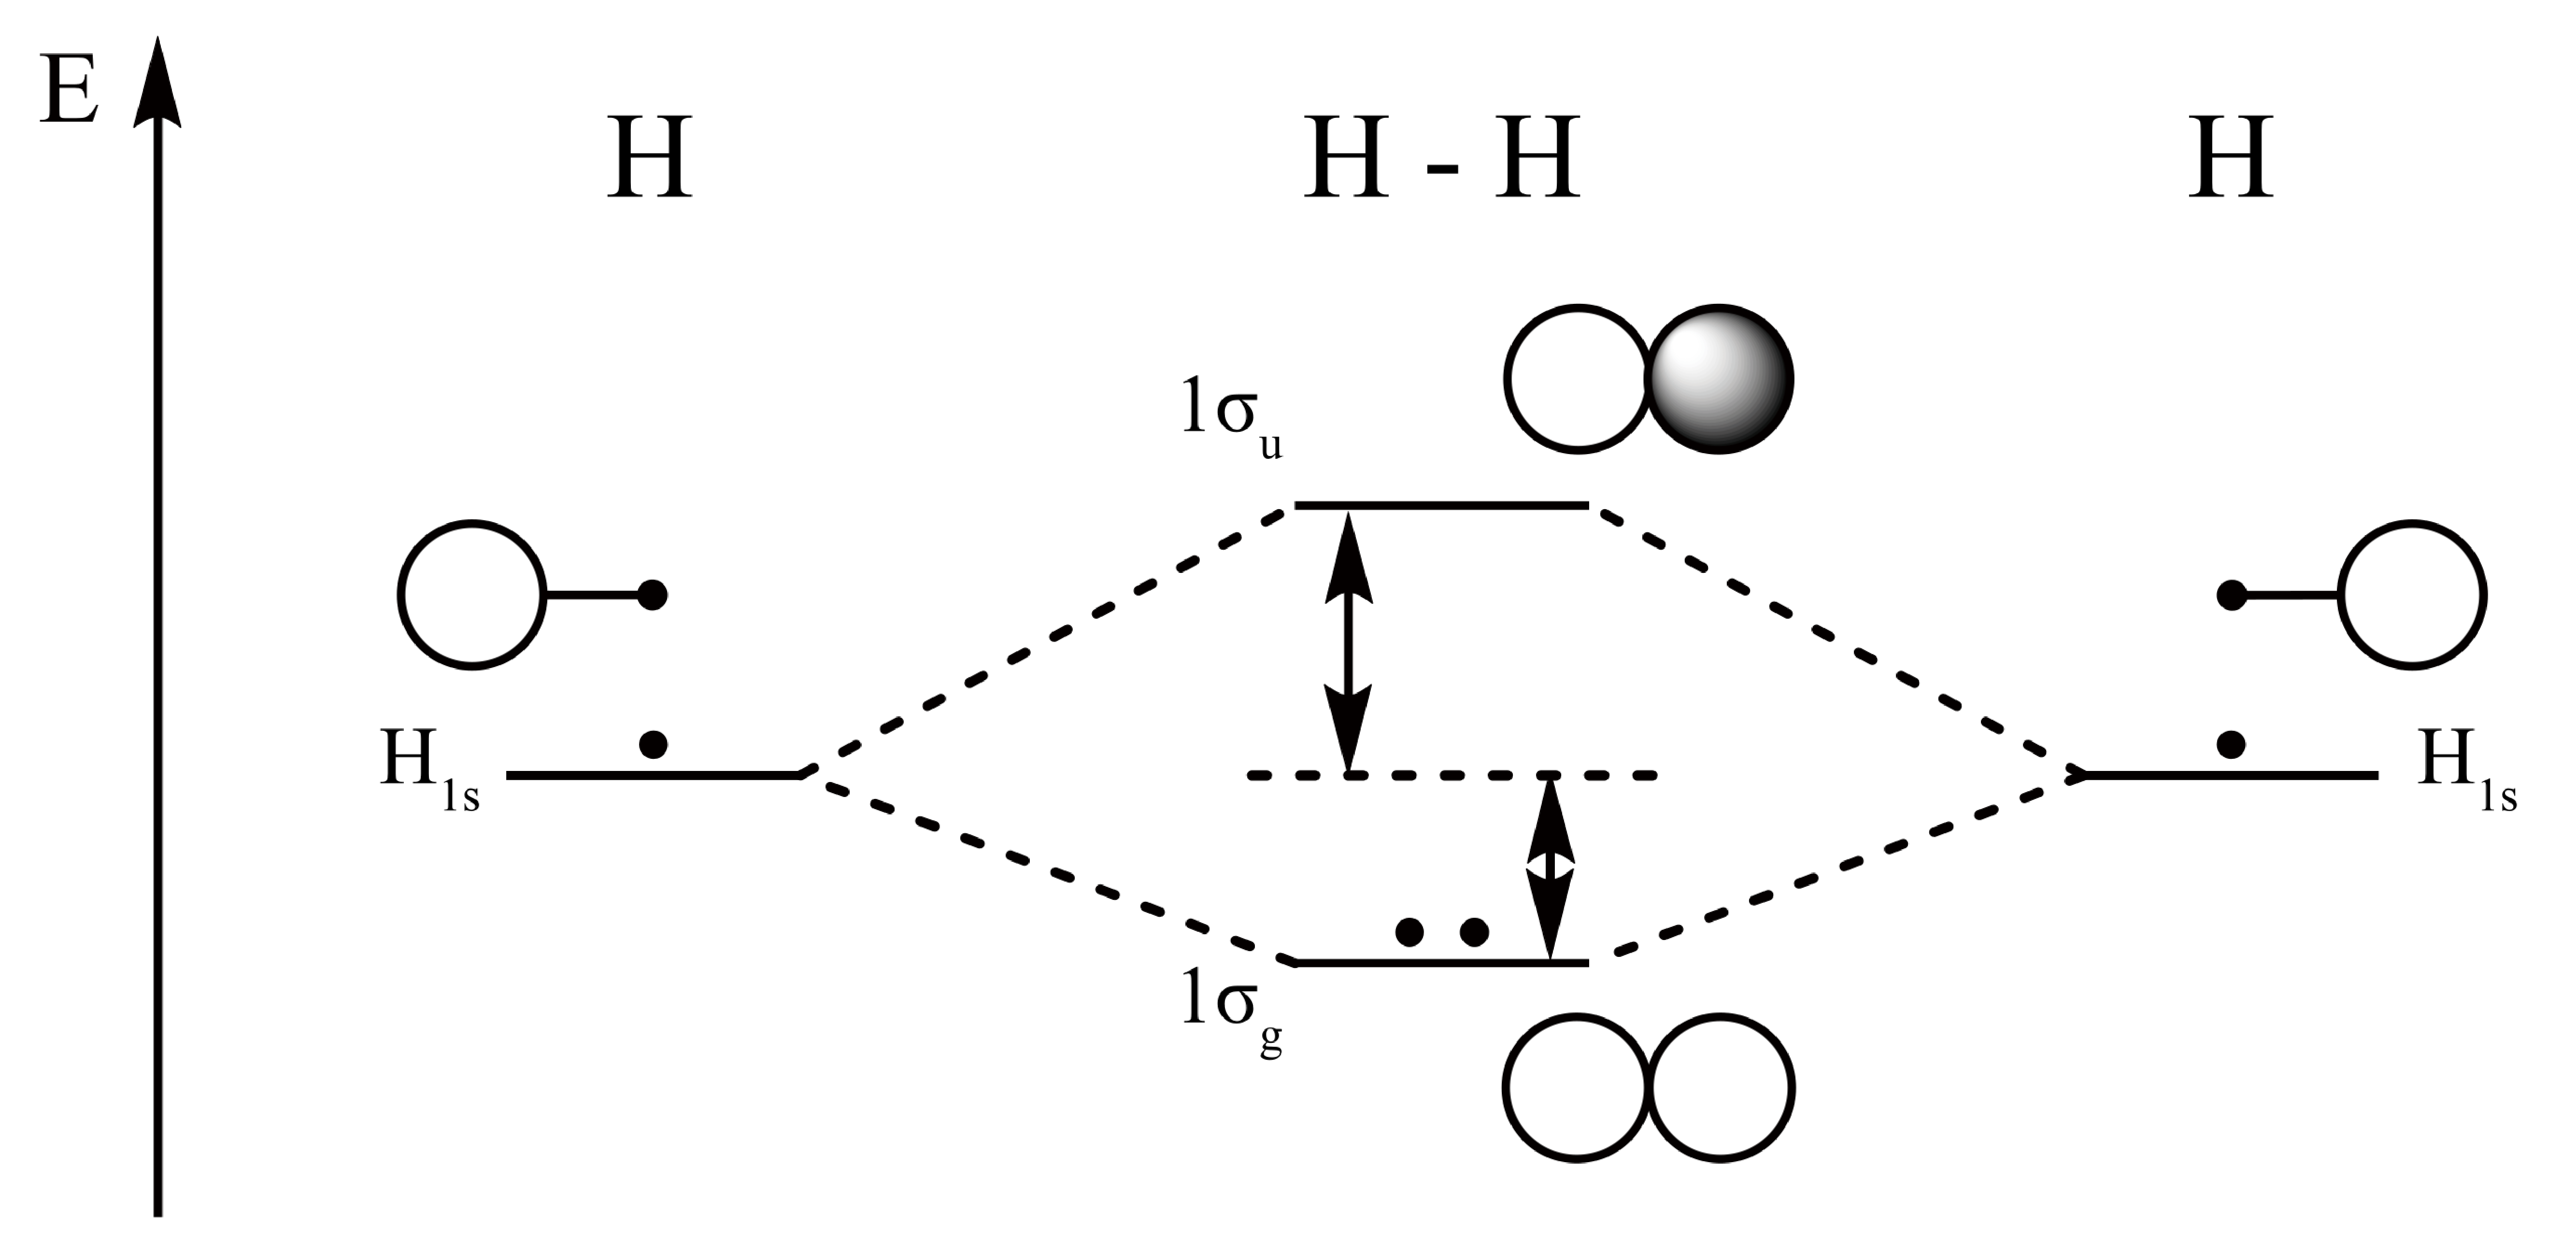
\includegraphics[width=0.6\linewidth]{Figures/h-orbital-diagram.pdf}
    \caption{MO diagram for dihydrogen. Reproduced from reference~\cite{h-orbital-diagram}.}\label{fig:h-orbital-diagram}
\end{figure}

In more complex polyatomic species, these MOs are most easily interpreted as eigenfunctions of the molecular Hamiltonian, and their energies are the corresponding eigenvalues. 
These orbitals describe the distribution of each electron throughout the molecule and hence the bonding within the molecule, but do not translate well into the more intuitive valence bond description of bonding that is most useful to chemists.
From a series of MOs, there is not an easy way to draw a Lewis structure of the molecule at hand.
This is because MOs tend to be highly delocalised throughout the molecule, which is obvious even in the relatively simple case of benzene (\cref{fig:benzene-mo}).

\begin{figure}
    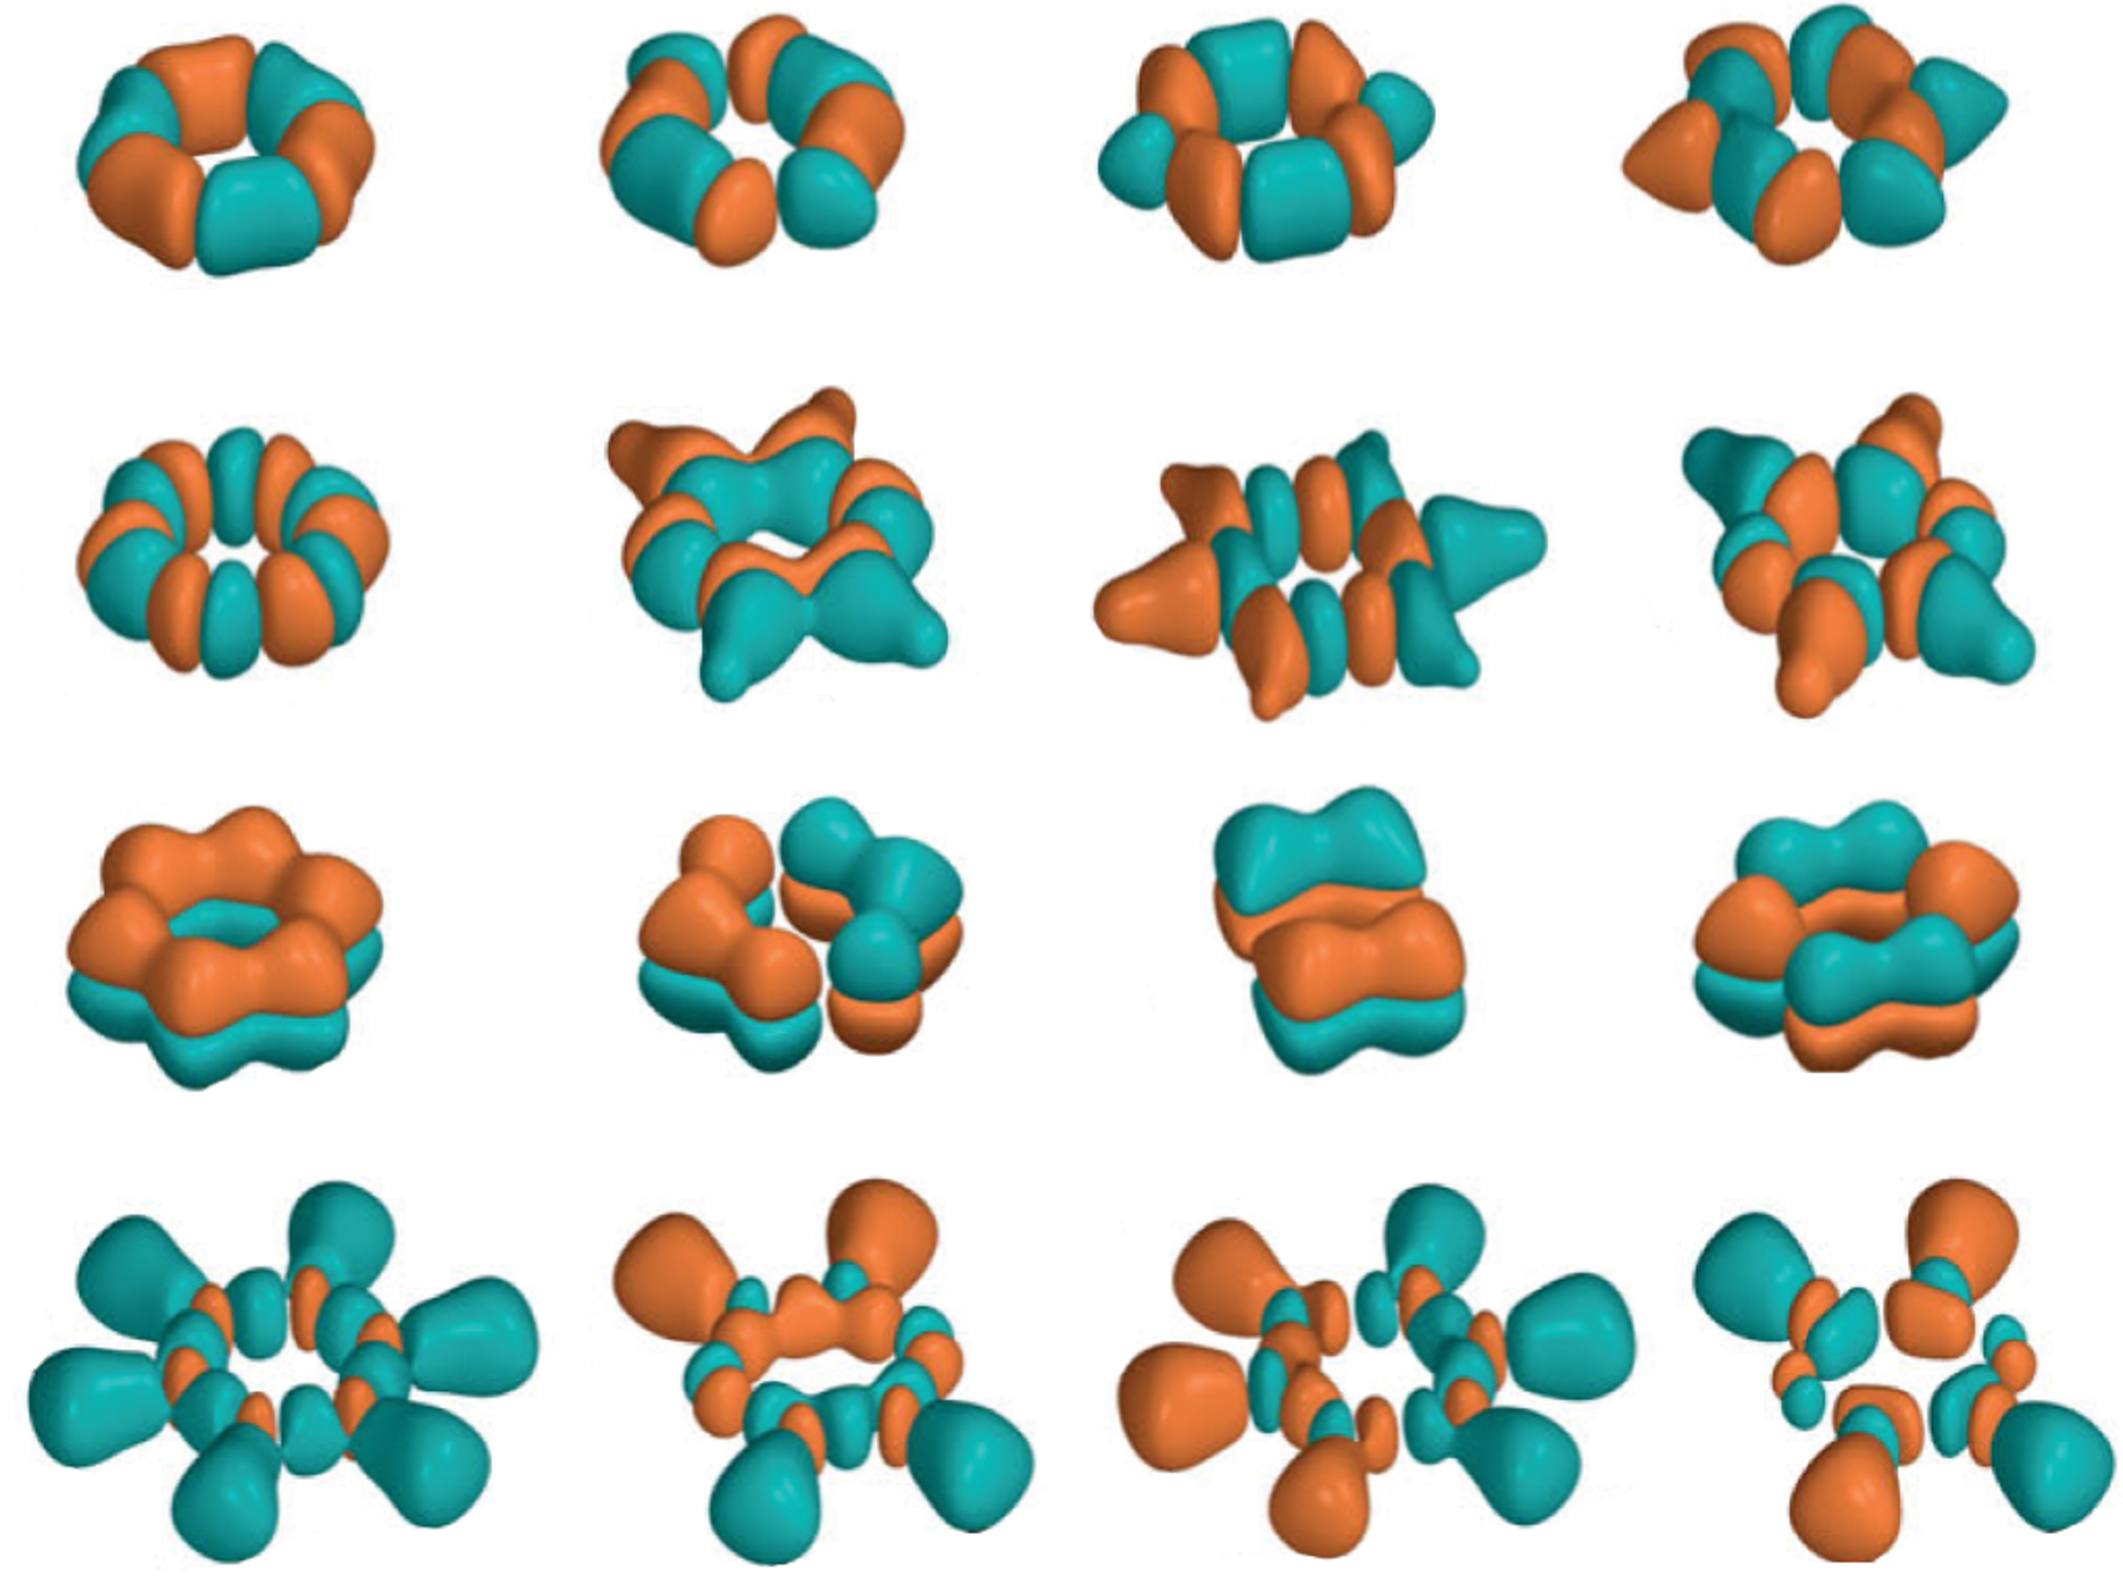
\includegraphics[width=0.8\linewidth]{Figures/benzene-mo.pdf}
    \caption{Molecular orbitals of benzene. Reproduced from reference~\cite{Luhmann2015}.}\label{fig:benzene-mo}
\end{figure}

The Natural Bond Orbital (NBO) scheme attempts to ameliorate this delocalisation, by transforming the molecular orbitals into NBOs which correspond to features found in a Lewis structure.\autocite{Reed1988}
These take the form of one centre and two centre elements (lone pairs and bonding orbitals respectively), which together form the optimal Lewis structure for a molecule.
The NBO scheme also provides a framework for non-Lewis features, such as non-valence electrons which are found in core NBOs.
As a consequence of the transformation from atomic orbitals to NBOs, higher energy two centre elements arise, which correspond to anti-bonding orbitals whose partial occupancy leads to reduction of bond order.
Rydberg NBOs complete the span of the NBO space, which are high energy, highly diffuse orbitals which typically contribute little to the overall chemistry of the system. 
Examples of NBOs in a simple molecule are shown in \cref{fig:nbos}

\begin{figure}
    \centering
    \begin{subfigure}{0.3\linewidth}
        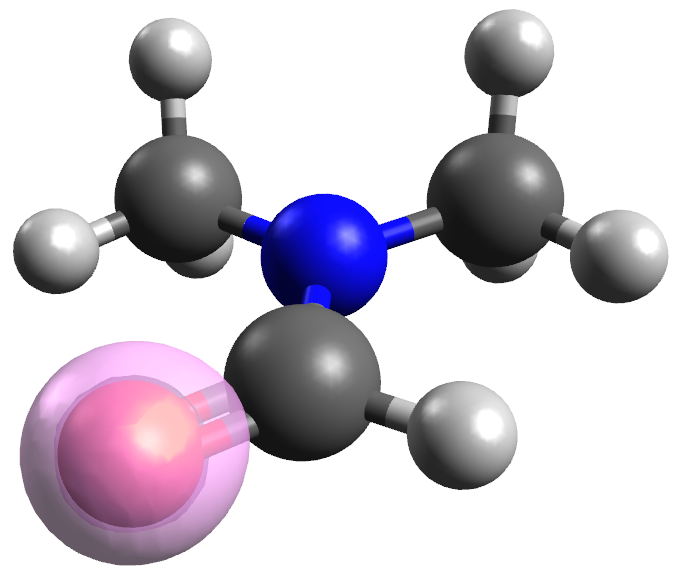
\includegraphics[width=\linewidth]{Figures/dmfnbo-core.png}
        \caption{Core NBO.}
    \end{subfigure}
    \begin{subfigure}{0.3\linewidth}
        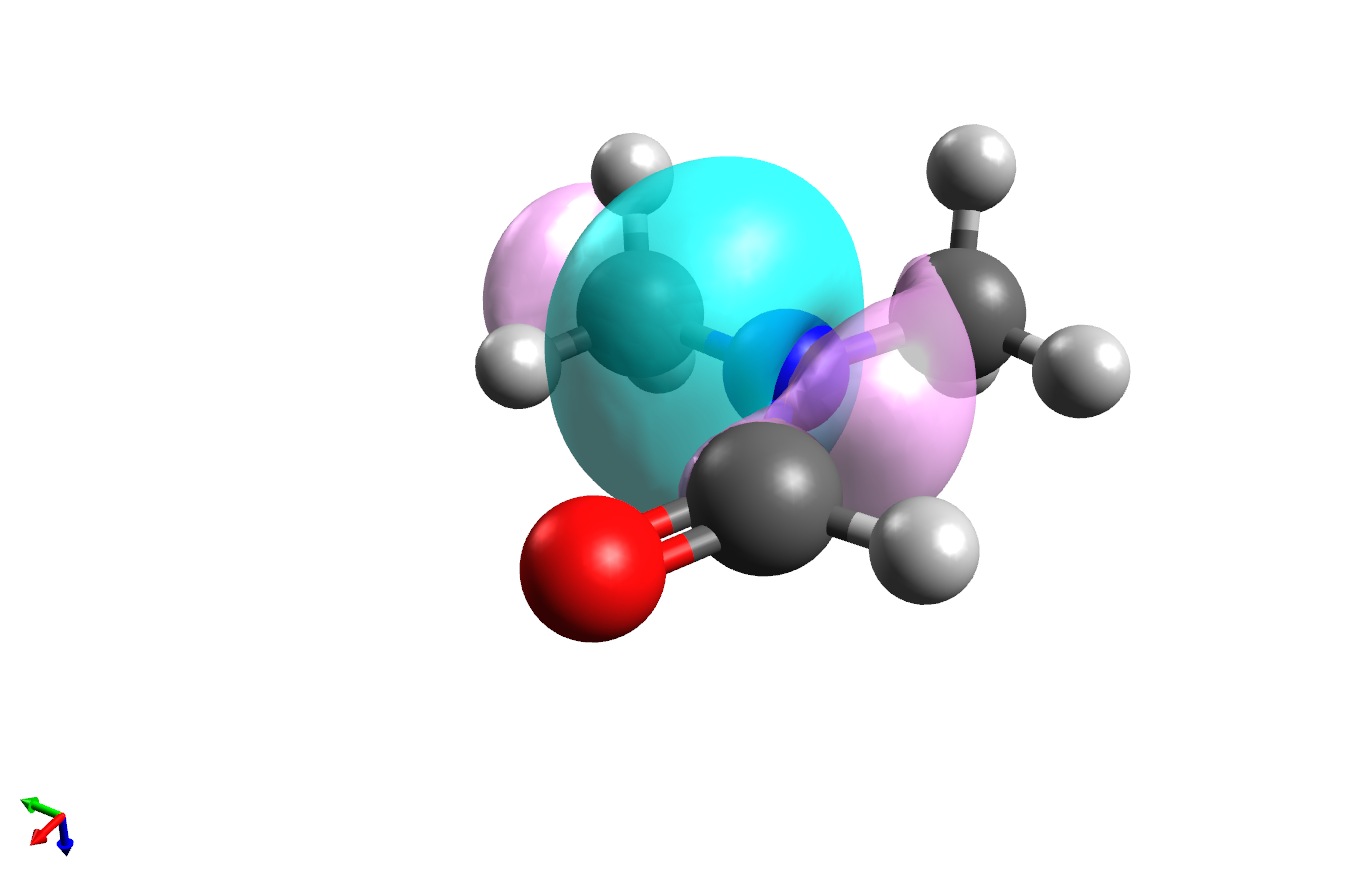
\includegraphics[width=\linewidth]{Figures/dmfnbo-sigma.png}
        \caption{$ \sigma $ bonding NBO.}
    \end{subfigure}
    \begin{subfigure}{0.3\linewidth}
        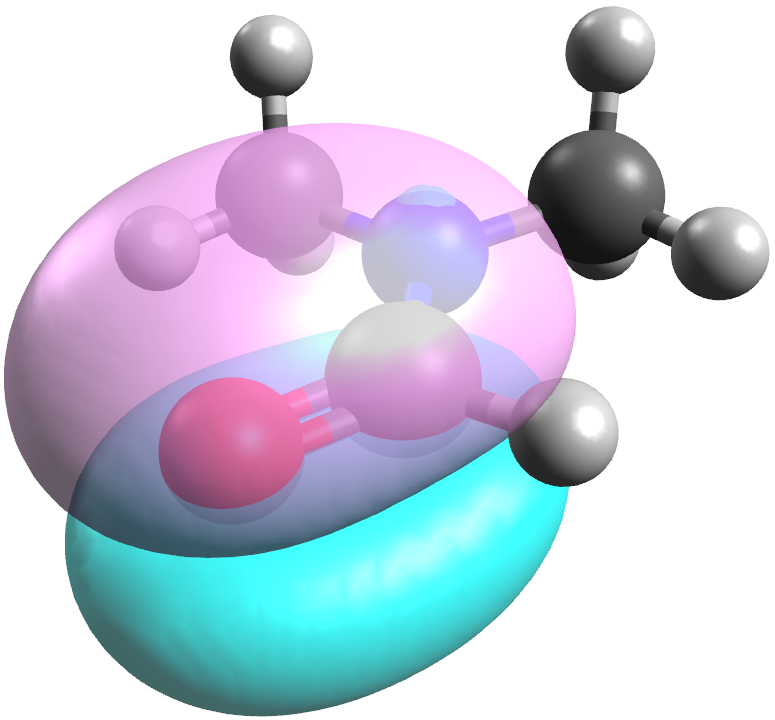
\includegraphics[width=\linewidth]{Figures/dmfnbo-pi.png}
        \caption{$ \pi $ bonding NBO.}
    \end{subfigure}

    \begin{subfigure}{0.3\linewidth}
        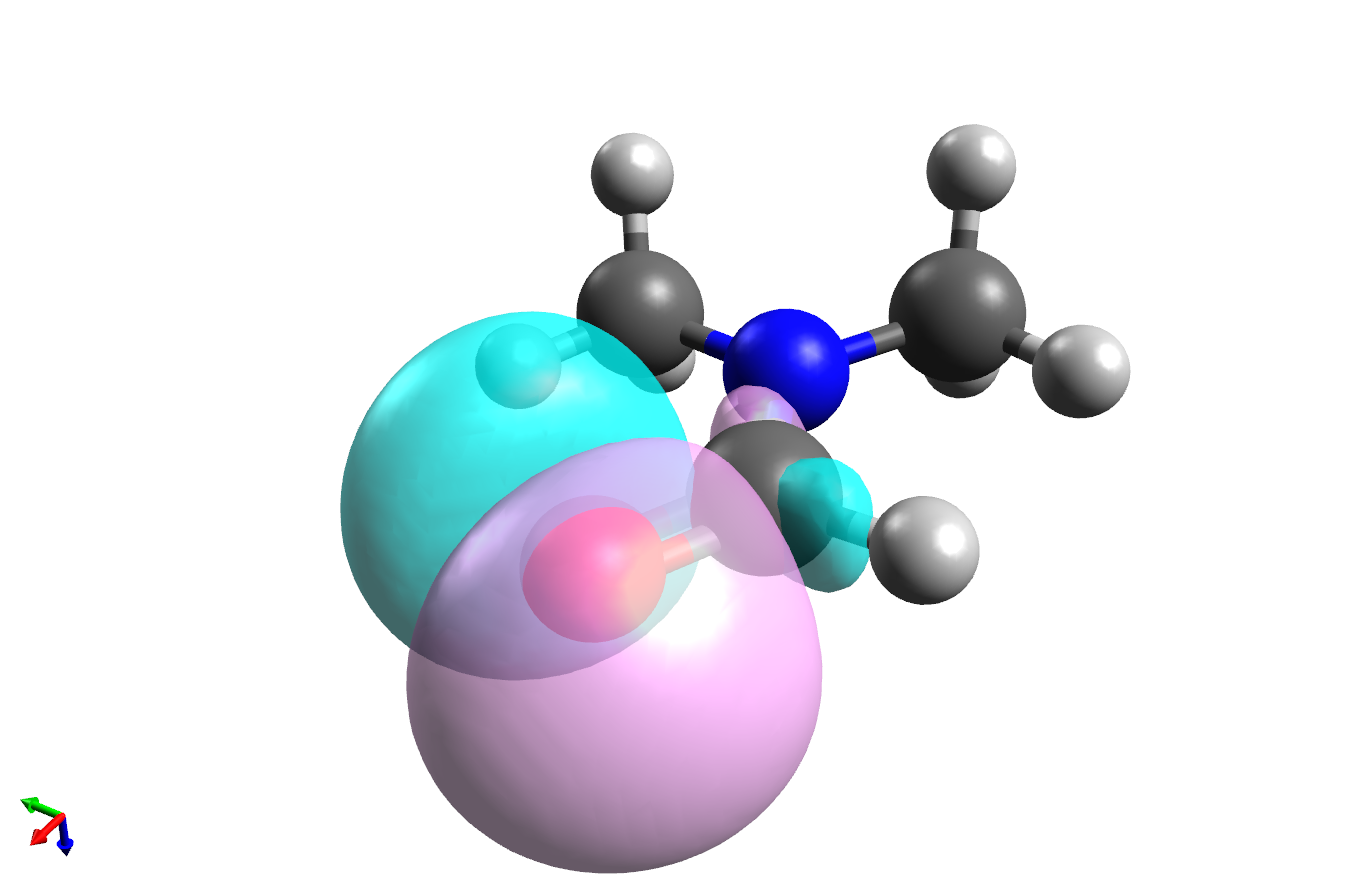
\includegraphics[width=\linewidth]{Figures/dmfnbo-n.png}
        \caption{Lone pair (n) NBO.}
    \end{subfigure}
    \begin{subfigure}{0.3\linewidth}
        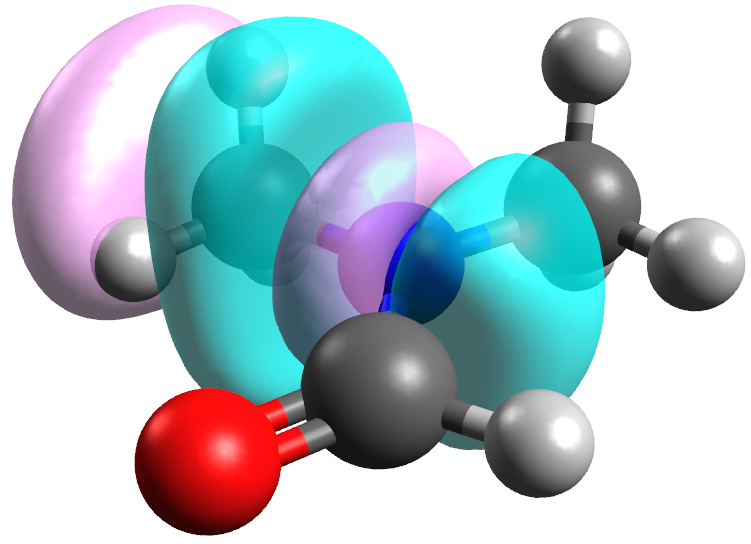
\includegraphics[width=\linewidth]{Figures/dmfnbo-sigmastar.png}
        \caption{$ \sigma^{\star} $ anti-bonding NBO.}
    \end{subfigure}
    \begin{subfigure}{0.3\linewidth}
        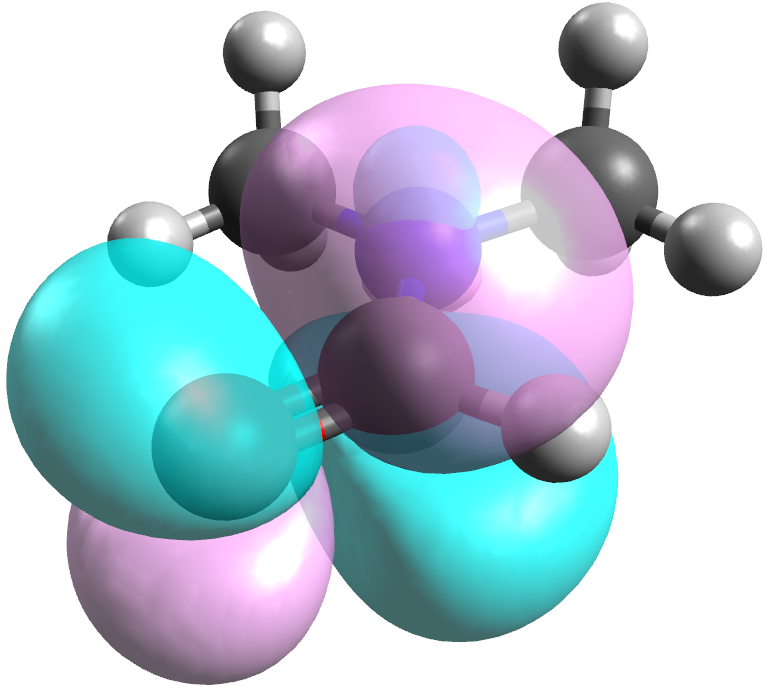
\includegraphics[width=\linewidth]{Figures/dmfnbo-pistar.png}
        \caption{$ \pi^{\star} $ anti-bonding NBO.}
    \end{subfigure}

    \begin{subfigure}{0.3\linewidth}
        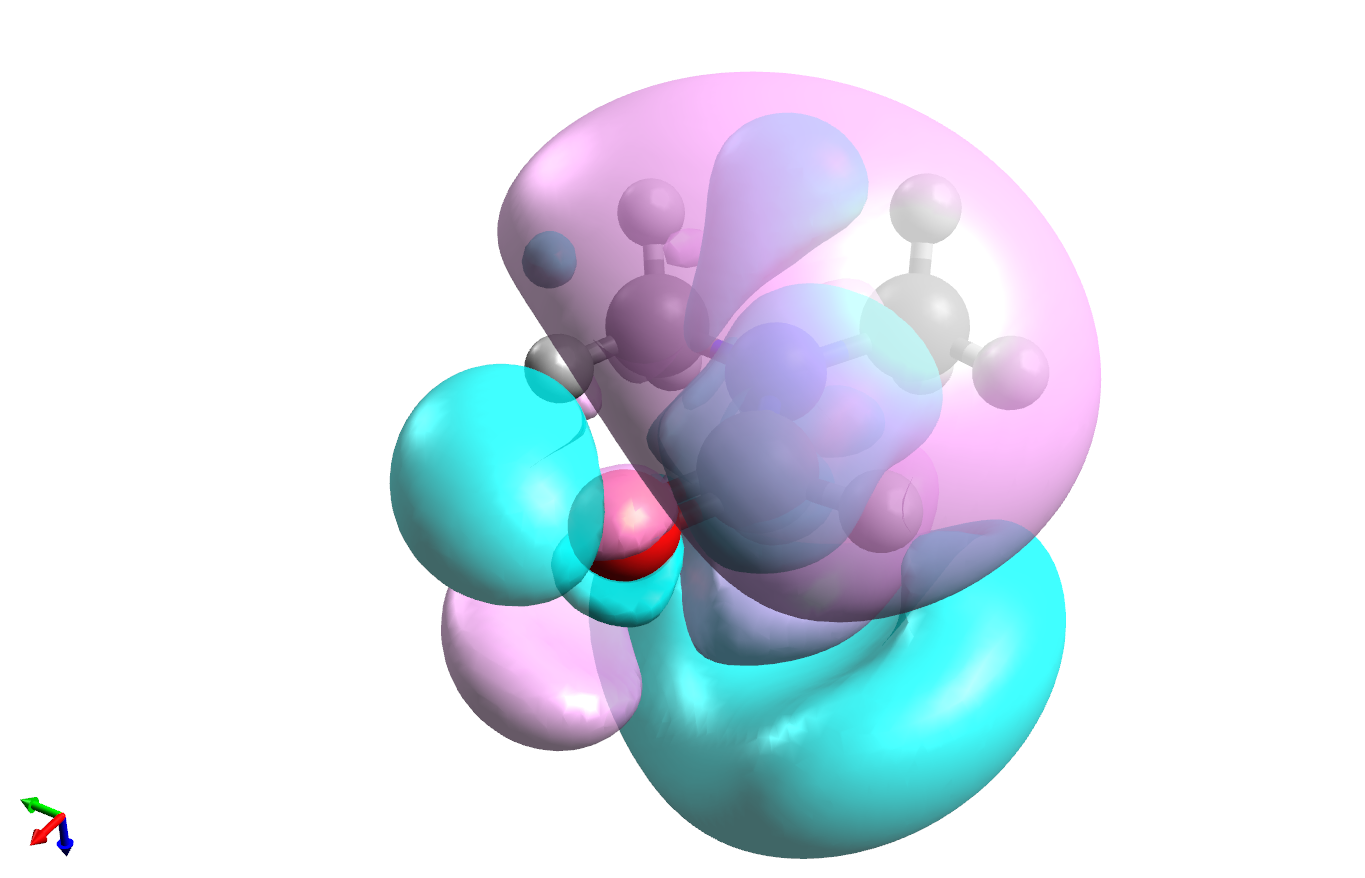
\includegraphics[width=\linewidth]{Figures/dmfnbo-rydberg.png}
        \caption{Rydberg NBO.}
    \end{subfigure}
    \caption{Representative Natural Bond Orbitals of a DMF molecule.}\label{fig:nbos}
\end{figure}

We use NBO theory to rationalise the hyperconjugative effects present in Ch-bonded complexes, namely, the $ \text{n}\rightarrow\sigma^{\star} $ overlap which appears to be present.
NBO analysis allows a numerical value to be assigned to the degree of this overlap, in terms of the formal number of electrons which are ``transferred'' from one orbital to the other.
The energies of each NBO can then be used to calculate the stabilisation afforded by a given delocalisation.

In summary, NBOs are a mathematical transformation of highly delocalised MOs into functions that correspond to the Lewis structure interpretation of chemical bonding.
Although this generates an ideal Lewis structure of a species, departures from this ideal (in the form of delocalisation and hyperconjugative effects) can be seen in decreased occupancy of bonding orbitals and increased occupancy of anti-bonding orbitals.
This allows for a mathematically rigorous and quantitative treatment of bonding, using familiar chemical concepts.

\subsection{Quantum Theory of Atoms In Molecules}
\label{sec:qtaim}
The Quantum Theory of Atoms In Molecules (QTAIM) is a description of bonding that is complimentary to that of NBO theory.\autocite{Bader1991}
Rather than describing bonds in terms of orbitals, it uses features of the electron density to define bonding.
This is particularly attractive as orbitals and wave functions are not observable quantities, whereas electron density is.
Indeed electron density can be measured directly through diffraction experiments (see \cref{sec:cd}).
It can also be calculated from a molecular wave function, which can itself be calculated by any number of methods.

To discuss QTAIM, we must first discuss some mathematical aspects of topology.
The fundamental quantity in QTAIM is the electron density $ \rho(\textbf{r}) $, which constitutes a scalar field over the molecule.
That is, every point in space has a single number representing the electron density at that point (see \cref{fig:dmf-rho} for an example).
Differentiating $ \rho(\textbf{r}) $ affords the gradient $ \nabla\rho(\textbf{r}) $, a measure of the local rate of change (in space) of the electron density.
$ \nabla\rho(\textbf{r}) $ is a vector quantity, with a magnitude and direction, which thus forms a vector field.
Differentiating $ \nabla\rho(\textbf{r}) $ again affords the second derivative of $ \rho(\textbf{r}) $, also called the Hessian $ \mathbf{H} $.
$ \mathbf{H} $ is a tensor quantity, which is most commonly represented as a $ 3\times3 $ matrix.
This is not easily represented as a field, but the three eigenvalues (components of the diagonalised Hessian) are useful quantities, which each represent the rate of change of $ \nabla\rho(\textbf{r}) $ at a given point. 
These are given the symbols $ \lambda_1 $, $ \lambda_2 $, and $ \lambda_3 $.
The sum of these eigenvalues is called the Laplacian of the electron density, which is given the symbol $ \nabla^{2}\rho(\textbf{r}) $.
Maps of $ \nabla^{2}\rho(\textbf{r}) $ can recover some chemical features of molecules that are reminiscent of the orbital structure, even though it is derived completely from the $ \rho(\textbf{r}) $ scalar field (\cref{fig:dmf-lapl}).

\begin{figure}
    \centering
    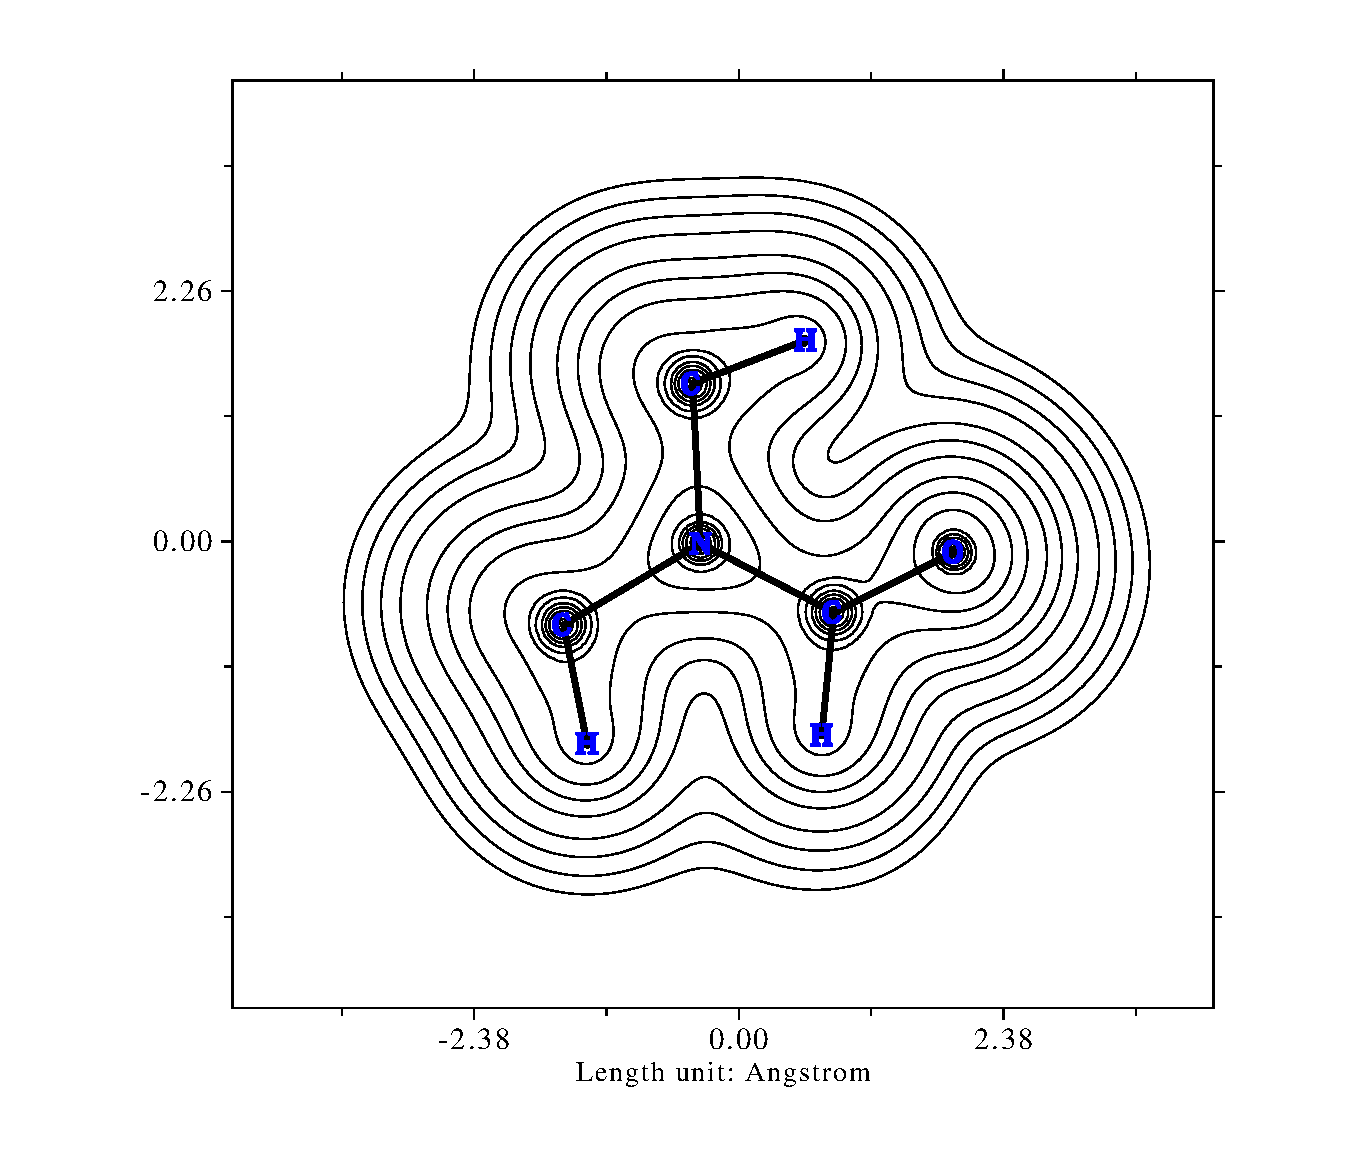
\includegraphics[width=0.48\linewidth]{Figures/dmf-dens-contour.pdf}
    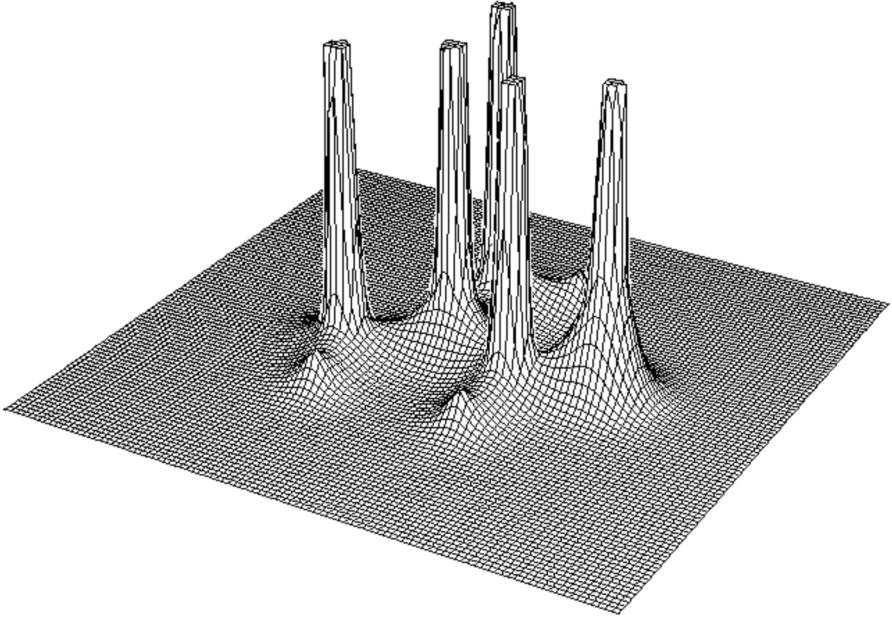
\includegraphics[width=0.48\linewidth]{Figures/dmf-dens-relief.pdf}
    \caption[Electron density $ \rho(\textbf{r}) $ in the plane of a DMF molecule.]{Electron density in the plane of a DMF molecule. The nuclei correspond to the large peaks, and bonds correspond to the ridges linking them.}\label{fig:dmf-rho}
\end{figure}

\begin{figure}
    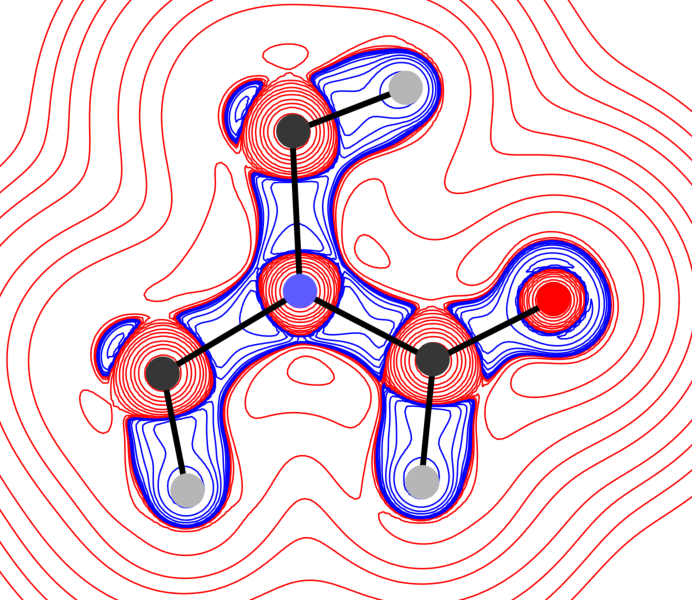
\includegraphics[width=0.48\linewidth]{Figures/dmf-lapl.pdf}
    \caption[Laplacian of the electron density $ \nabla^{2}\rho(\textbf{r}) $ of DMF.]{Laplacian of the electron density $ \nabla^{2}\rho(\textbf{r}) $ of DMF.\@ Positive values are shown in red and negative values in blue. $ \nabla^{2}\rho(\textbf{r}) $ can be seen to recover the shell structure of atoms, as well as chemical features such as bonds and lone pairs.}\label{fig:dmf-lapl}
\end{figure}

A QTAIM atom is defined by a volume bounded by a surface of zero electron density gradient flux (\cref{fig:dmf-gradient}).
That is, there are no field lines of $ \nabla\rho(\textbf{r}) $ crossing the surface.
A molecule can thus be partitioned into atoms, each of which is strictly additive and transferable.
Furthermore, atomic contributions to molecular properties can be uniquely defined.
This is similar to the idea of functional groups in organic chemistry.
In the same way a carboxylic acid functional group can be transferred between molecules while retaining its characteristic properties (its acidity), a QTAIM atom can also be transferred, as its properties depend \emph{only} on the topology of the electron density.

\begin{figure}
    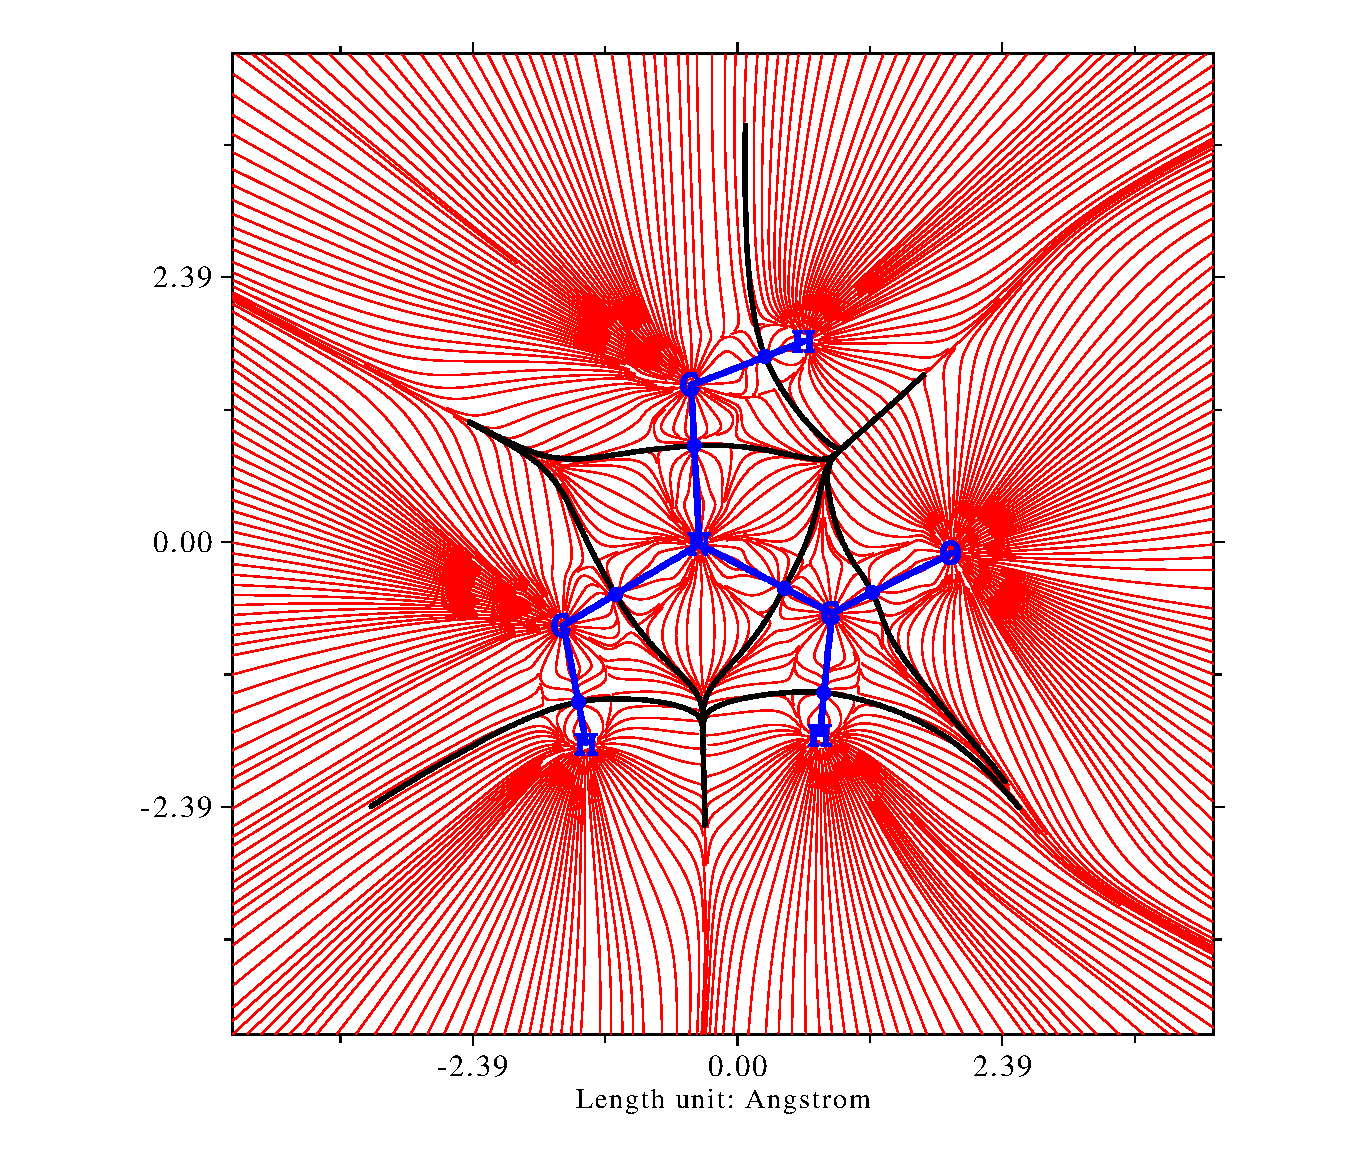
\includegraphics[width=0.48\linewidth]{Figures/dmf-grad.pdf}
    \caption[Electron density gradient $ \nabla\rho(\textbf{r}) $ vector field of DMF.]{Electron density gradient $ \nabla\rho(\textbf{r}) $ vector field of DMF.\@ All field lines (red) converge on the nuclei, and asymptotically approach the zero flux surfaces (black lines) which bound the QTAIM atoms. Bond paths and critical points are shown in blue.}\label{fig:dmf-gradient}
\end{figure}

Each QTAIM atom is associated with a local maximum of electron density which is located at the nucleus.
At this point $ \nabla\rho(\textbf{r}) $ is zero, so it is termed a critical point.
As it is a maximum, $ \rho(\textbf{r}) $ will decrease in all directions, therefore all three eigenvalues of $ \mathbf{H} $ will be negative.
These atomic critical points are therefore termed $ (3,-3) $ critical points, as they exist in three dimensional space and have three negative eigenvalues.

\begin{figure}
    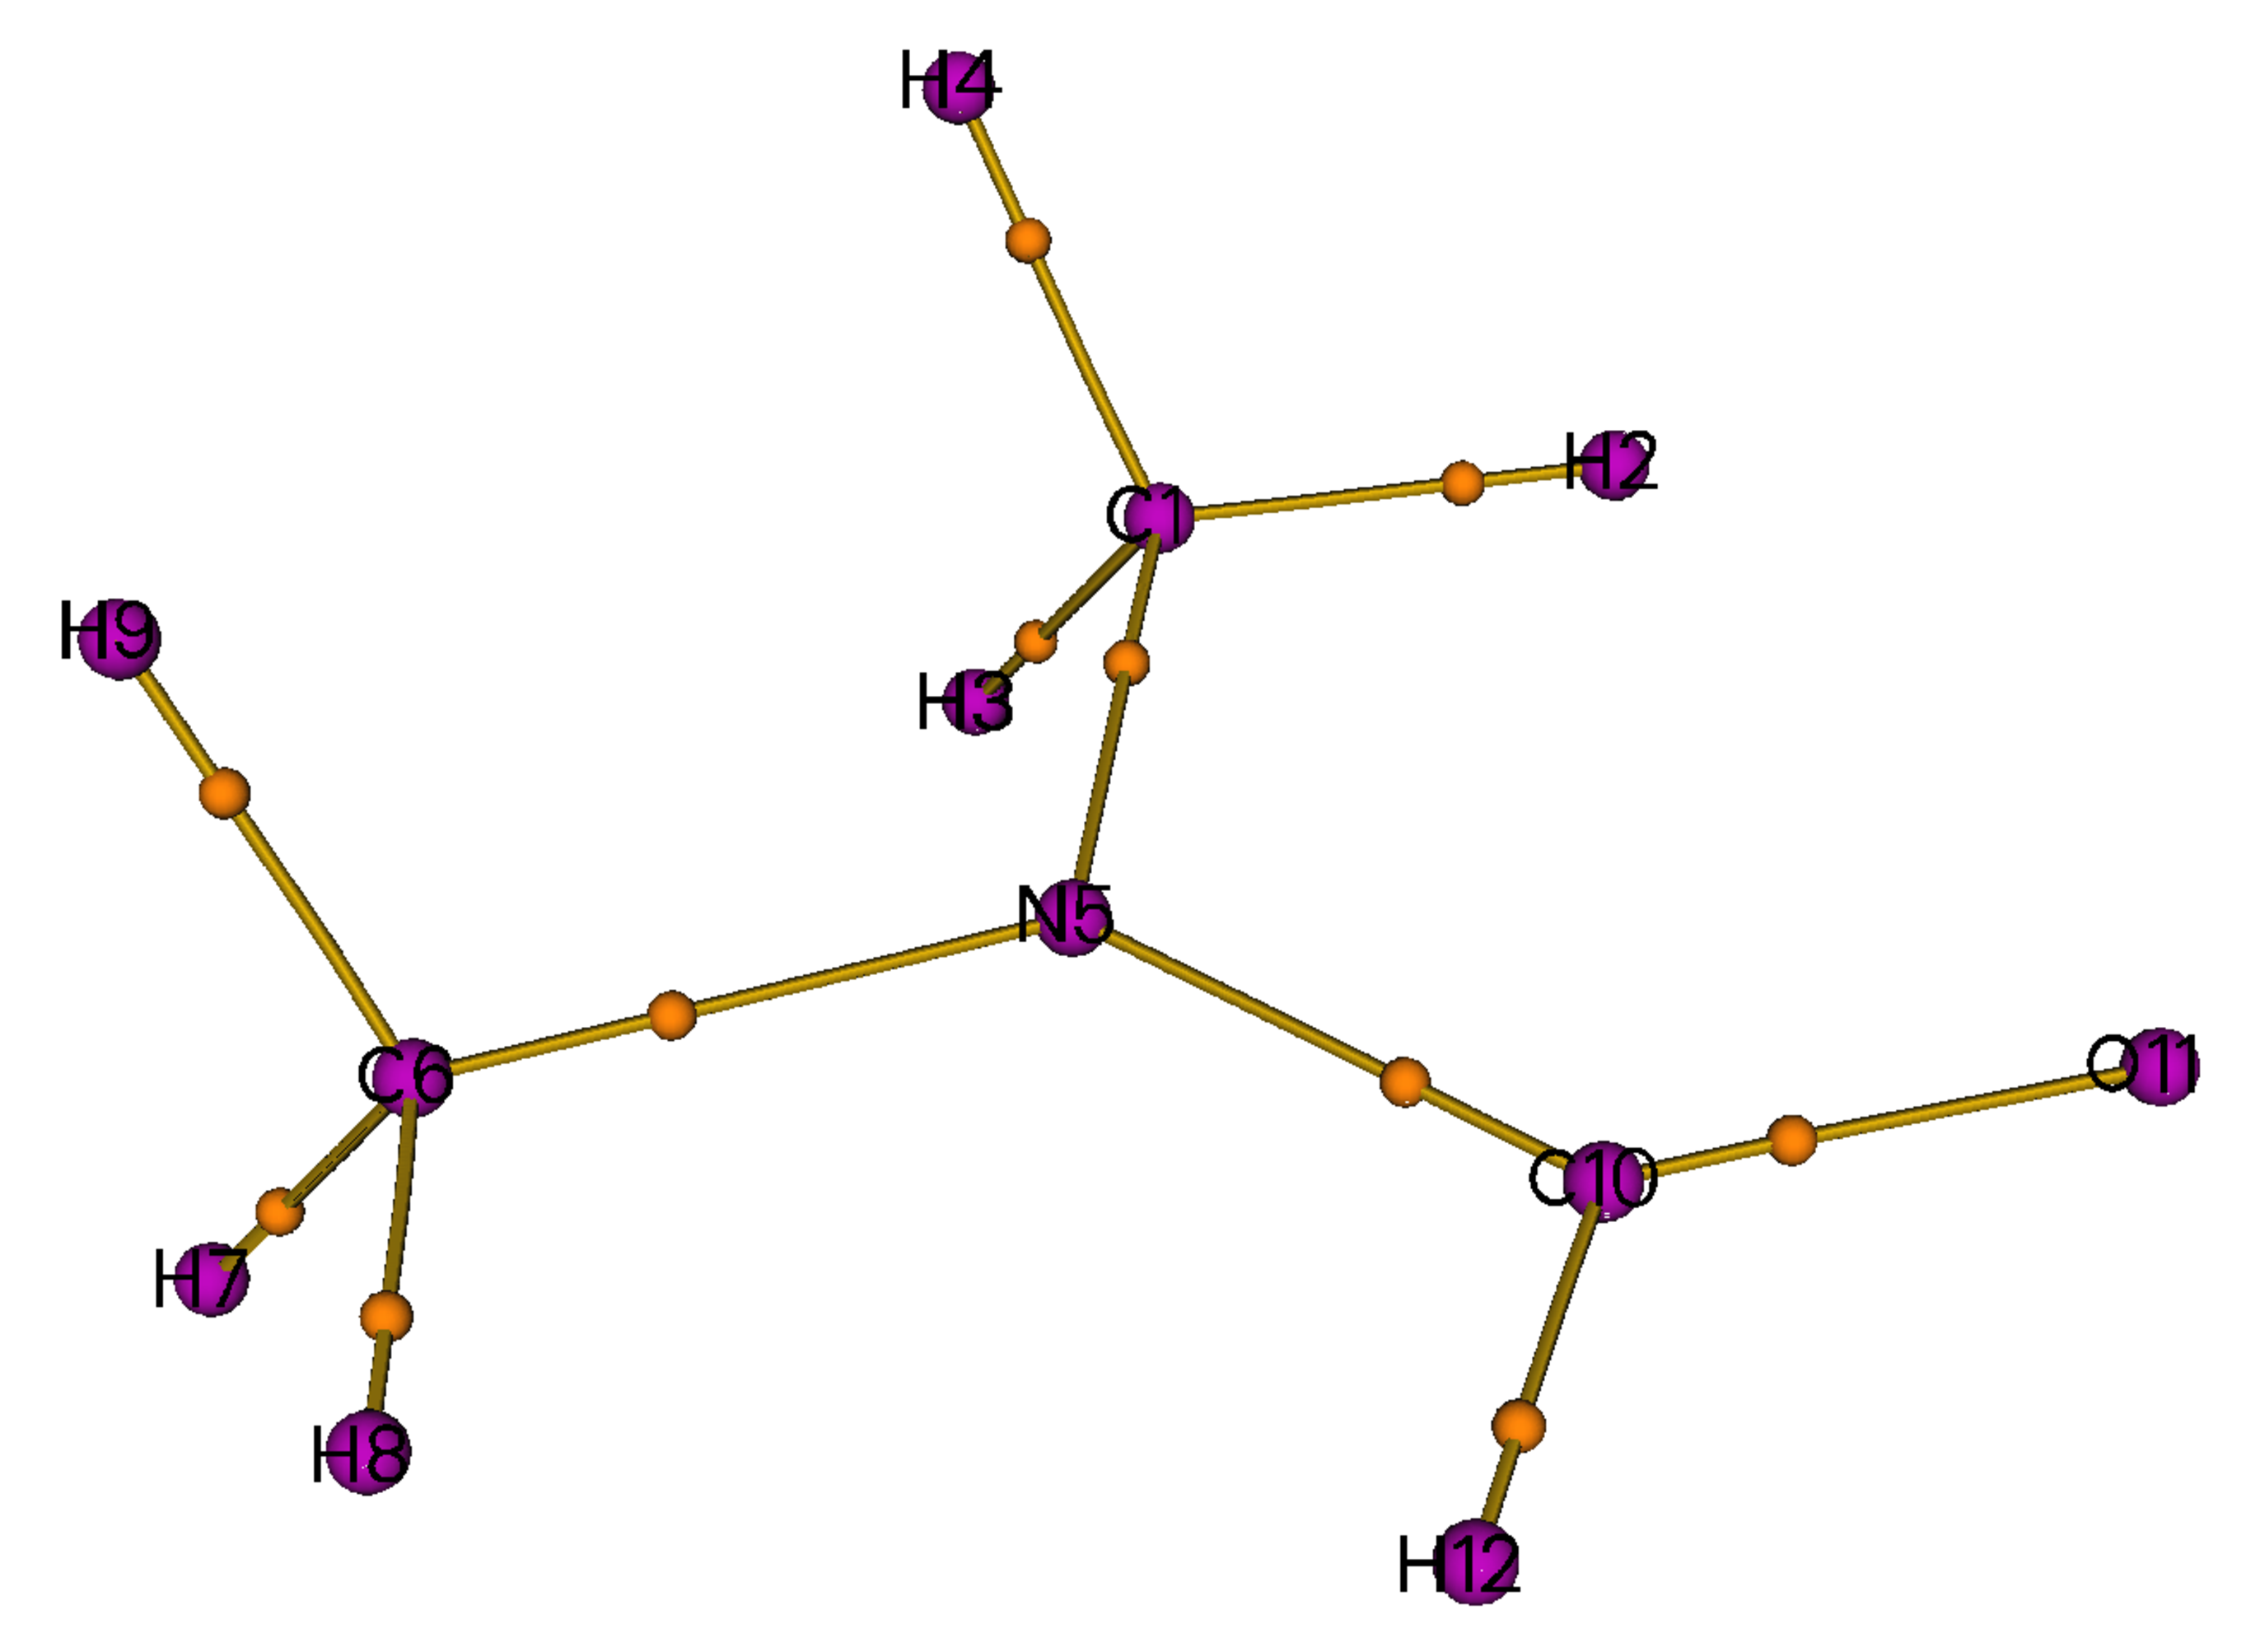
\includegraphics[width=0.45\linewidth]{Figures/dmf-cp.pdf}
    \caption[Critical points of DMF.]{(3,-3) (pink), and (3,-1) (orange) critical points of DMF.\@ Bond paths are shown in yellow.}\label{fig:dmf-cps}
\end{figure}

Nuclei are not the only place critical points are found (where $ \nabla\rho(\textbf{r}) $ is zero).
Atomic critical points contained within neighbouring QTAIM atoms (sharing a common zero gradient flux surface) are linked by lines along which $ \rho(\textbf{r}) $ decreases in the two directions perpendicular to the line.
In two dimensions this can be visualised as a ridge connecting two mountain peaks.
This line is termed a bond path, as the presence of such a line is a prerequisite for bonding to occur (although the reverse is not necessarily true).
At the point where the bond path crosses the zero gradient flux surface there will be another critical point where $ \nabla\rho(\textbf{r}) $ is zero.
This type of critical point is called a bond critical point (BCP) or $ (3,-1) $ critical point, as $ \rho(\textbf{r}) $ decreases in two directions but increases in one direction (along the bond path).
$ \mathbf{H} $ at a $ (3,-1) $ critical point therefore has two negative eigenvalues and one positive eigenvalue.
An example of a molecular structure derived from the critical points and bond paths is shown in \cref{fig:dmf-cps}.
There are also critical points found at the centres of rings (ring or $ (3,1) $ critical points) or at the centres of cage-like structures (cage or $ (3,3) $ critical points), however these are not discussed in this thesis.

As stated before, the presence of a bond path and BCP is necessary but not sufficient to say there is chemical bonding occurring.
In this work we therefore use the presence of a bond path, as measured from experimental electron density, to support our claim that Ch-bonding is occurring.
We also use the values of properties related to $ \rho(\textbf{r}) $ at the BCP to characterise the type of bonding that we observe.
Although this does not replace a proper energy decomposition analysis, certain types of interaction have characteristic values of $ \rho(\textbf{r}) $ and $ \nabla^{2}\rho(\textbf{r}) $ at the BCP.\@ Covalent bonds are characterised by accumulation of electron density between the nuclei, and this is reflected in relatively large values for $ \rho(\textbf{r}) $, and a large and negative value of $ \nabla^{2}\rho(\textbf{r}) $.
Closed shell interactions, on the other hand, do not show this accumulation of charge, so at the BCP $ \rho(\textbf{r}) $ is small, and $ \nabla^{2}\rho(\textbf{r}) $ is positive.

In contrast to NBO theory, QTAIM is a complementary, but equally quantitative and mathematically sound, interpretation of bonding in chemical species.
It has the unique benefit of being grounded solely in the experimentally observable property of the electron density, while still being able to recover chemically intuitive aspects of bonding.

\section{X-ray crystallography}
Single crystal x-ray crystallography is the main experimental technique used in this work.
It allows unambiguous determination of the structure of compounds (including stereochemistry), and  extremely accurate measurement of geometric parameters such as bond lengths.
Practically speaking, a structure is determined by mounting a single crystal of a compound on a goniometer which can rotate the crystal through any orientation, then observing the position and intensity of diffracted x-ray beams.
Rotating the crystal allows different diffraction spots to be observed, and a more complete dataset to be collected.
The position of the diffraction spots provides information about the size and shape of the unit cell, and the intensities provide information about the internal structure i.e.\ the locations of the atoms in the unit cell.
A full discussion of the mathematics of diffraction is outside the scope of this thesis, but the interested reader is referred to \citetitle{Stout1989} by \citeauthor{Stout1989}.\autocite{Stout1989}

\subsection{Charge density refinement}\label{sec:cd}
Fundamental to the technique of x-ray structure determination is the process of refinement, by which parameters of the model (typically the molecular geometry) are optimised to reproduce the observed intensity data as well as possible.
Mathematically, this is performed as a least-squares optimisation, where the function
\begin{equation}
    \sum^{m}_{r=1} w_{r} {\left(I_{\mathrm{obs}, r} - I_{\mathrm{calc}, r} \right)} ^{2}
\end{equation}
is minimised, where $ I_{\mathrm{obs}, r} $ corresponds to the observed intensity, and $ I_{\mathrm{calc}, r} $ corresponds to the intensity calculated from the model by Fourier transform.
$ w_{r} $ is a weighting function used to reflect the confidence in any given observed data point.

Assuming the measured intensities are free of any error,\footnote{This is practically never the case, but careful measurement and modern corrections can approach this limit.} this function could theoretically be minimised to zero i.e.\ the model is a complete and true representation of the crystal.
The question then becomes, how do we determine $ f_{\mathrm{calc}, r} $ from our model?
To answer this, we must consider what our model actually \emph{is}.

The simplest refinement model consists of atomic coordinates for each atom, plus an overall scale factor (for now we will neglect the anisotropic displacement parameters and chemical occupancies).
However, in order to calculate $ f_{\mathrm{calc}, r} $ by Fourier transform, we must introduce some description of what the atoms which we are locating ``look like''.
This forms a hidden, but still crucially important, part of the model.
Typically, atoms are described in reciprocal space as spherically symmetric functions whose contribution to $ f_{\mathrm{calc}, r} $ is only dependent on $ (\sin\theta)/\lambda $ (\cref{fig:scatterf}).
This is a consequence of the fact that x-rays are scattered by the \emph{electron cloud} of the atom.\footnote{X-rays have much less energy than the mass-energy of subatomic particles, and so are scattered in the low energy limit of Compton scattering, known as Thompson scattering.
The scattering power of a particle is inversely proportional to the square of its mass, so the massive nuclei contribute negligibly to scattering compared to electrons.}
At $ (\sin\theta)/\lambda = 0 $ the scattering factor is equal to the number of electrons in the atom.
However, the finite size of the electron cloud causes destructive interference and attenuation of the scattering factor as $ (\sin\theta)/\lambda $ increases, as x-rays scattered from one side of the electron cloud will be out of phase with those scattered from the other side.
Contrast this with neutron diffraction, where the neutrons are scattered predominantly by the point-like nucleus, affording a flat scattering function in reciprocal space.
There is almost no destructive interference, and thus neutron crystallography is characterised by an abundance of strong high angle data.
The scattering factor functions for all elements of the periodic table (and many ions) have been calculated based on theoretical electron densities from Hartree-Fock wave functions, and the results are available in the International Tables.\autocite{IntTabCIntensityofdiffractedintensities}
These functions are mercifully incorporated in crystallographic refinement software, shielding them from the user.

\begin{figure}
    \centering
    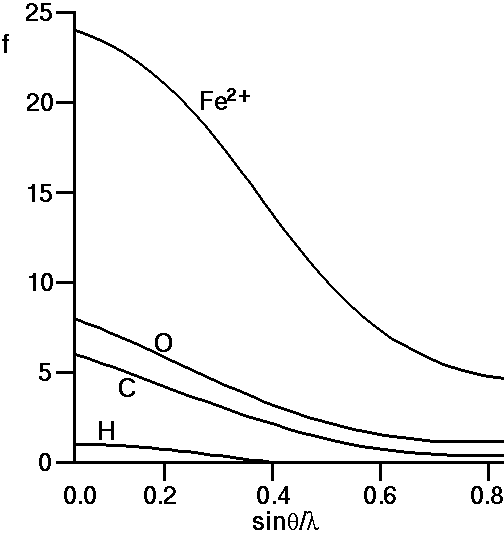
\includegraphics[width=0.5\linewidth]{Figures/scatterf.png}
    \caption{Scattering factors for some atoms as a function of $ (\sin\theta)/\lambda $.}\label{fig:scatterf}
\end{figure}

From the above discussion, one major shortcoming of this approach should be clear.
Namely, that the electron density of bonded atoms is \emph{not} spherically symmetric.
Perturbations such as bonding electron density, lone pairs, and indeed $ \sigma $-holes can, and do, affect the observed scattering factors of atoms, which are not taken into account in typical refinement software.
An extreme case of this, and one that is familiar to any crystallographer, is that of the hydrogen atom.
As the lightest element with only one electron, perturbations due to bonding have an enormous effect, such that the typical \ce{C-H} bond length is underestimated by some 0.13~\AA.\autocite{Cooper2010}
A subtler but more interesting manifestation of this was identified in 1968 by \citeauthor{Coppens1968EvidenceEffects}.\autocite{Coppens1968EvidenceEffects}
X-ray and neutron structures were determined for a crystal of 1,3,5-triazine, and inspection of the difference (a so-called $ \mathrm{X} - \mathrm{N} $ map) revealed unusual systematic variations in the anisotropic displacement parameters.
The nitrogen atoms were deformed radially to the ring, while the carbon atoms were deformed tangentially (\cref{fig:x-n-coppens}).
This is chemically intuitive, as we would expect the lone pairs of the nitrogens to extend radially, while the $ \pi $-electrons of the carbon atoms would form a ring.
The fact that these deformations were incorporated into the anisotropic displacement parameters in the x-ray structure highlights a deficiency of the typical method of refinement.

\begin{figure}
    \centering
    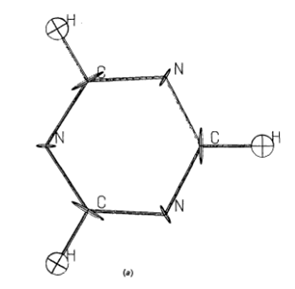
\includegraphics[width=0.5\linewidth]{Figures/x-n-coppens.png}
    \caption[Structure of 1,3,5-triazine.]{$ \mathrm{X} - \mathrm{N} $ map of 1,3,5-triazine, reproduced from \citeauthor{Coppens1968EvidenceEffects}.\autocite{Coppens1968EvidenceEffects}}\label{fig:x-n-coppens}
\end{figure}

Evidence for aspherical atoms can even be traced back to seminal studies performed by \citeauthor{Bragg1920}, in which the famous 222 reflection of a diamond crystal was observed.
The 222 reflection is a systematic extinction of the $ Fd\bar{3}m $ space group to which diamond belongs, but its absence is based on the assumption of spherical atoms.
In diamond, the carbon atoms are actually tetrahedral in form due to the bonding electron density, which lowers the space group symmetry and causes the 222 reflection to be present, though very weak.\autocite{Bragg1920}
Though cutting edge for the time, Bragg's experiment was rather primitive, and multiple scattering likely contributed some intensity to the observed 222 reflection.
The observation was nonetheless correct, and the tetrahedral nature of the carbon atoms in diamond has subsequently been proven time and time again.

Although such perturbations generally only manifest in very high quality structures (aspherical atoms are typically the least of a crystallographer's worries), a number of methods have been proposed to improve refinements, and indeed gain further chemical knowledge from the experimentally determined aspherical electron density.
A simple approach is the use of tabulated aspherical scattering factors for atoms of distinct chemical types.
An example of this is the ELMAM2 database, developed by Jelsch and co-workers.\autocite{Domagaa2012}
The ELMAM2 database consists of experimentally derived scattering factors for all common atom types, with a focus on those found in amino acids and peptides.
A refinement using this database would begin by assigning a type to each atom, which can be done relatively easily using bonding geometries from a more primitive refinement.
This can afford substantial improvement in refinement statistics by providing a more accurate model, at a very modest computational cost.
The obvious drawback of this approach is that the scattering factors must already be tabulated, and the enormous diversity beyond the biochemically important C, H, N, and O precludes the assembly of a truly comprehensive database.
Furthermore, as the scattering factors are pre-tabulated, there is little chemical information that can be extracted from the model beyond somewhat improved precision in geometric parameters.

An improved approach is to compute scattering factors on a case-by-case basis.
This is the rationale behind Hirshfeld Atom Refinement (HARt), first developed by \citeauthor{Jayatilaka2008}.\autocite{Jayatilaka2008}
HARt is an iterative procedure in which the atomic coordinates from a spherical atom refinement (perhaps after correcting \ce{C-H} bond distances) are used to variationally calculate a wave function, from which is calculated an electron density and thus scattering factors.
These new scattering factors improve the model after refinement, from which is calculated a \emph{new} wave function, and so on until the cycles of least squares refinement and wave function calculations converge.
Clearly this repeated calculation of a wave function is computationally expensive, with even relatively simple molecules taking minutes.
Fortunately, however, even very inexpensive levels of theory tend to generate sensible densities for the ground state.
An advantage over the database approach is that one can capture unusual effects in the electron density (such as various non-bonding interaction), provided that they are correctly modelled by the underlying quantum chemistry theory used to generate the wave function.
However this raises a philosophical question: what exactly we are hoping to get out of this procedure?
It can certainly provide improved refinement statistics, including anisotropic refinement of hydrogens in agreement with neutron data, but if we are seeking chemical information about the system, we might as well simply use a gas-phase optimised wave function and dispense with the crystallography.

Related to this is the field of quantum crystallography, which differs somewhat in motivation, if not in methodology.
Quantum crystallography is concerned with extracting a wave function from diffraction data, rather than using a wave function to improve a crystallographic model.
Clearly there is significant overlap.
One method takes inspiration from perturbation theory, where, as in MP2, the Hartree-Fock wave function is taken as the zeroth order approximation.
The diffraction data is then used to construct a perturbative term, which introduces a degree of correlation to the wave function, bringing it closer to the truth (at least within the Born-Oppenheimer approximation).\autocite{Weiss1962}
Even with the power of modern computers, this is not an easy task, and quantum crystallography remains an active and exciting area of research.
It is also worth mentioning the x-ray constrained wave function method developed by \citeauthor{Grimwood2003}.\autocite{Grimwood2003}
This is simply a Hartree-Fock wave function calculations that is constrained via a Lagrangian multiplier to reproduce the observed intensities in the experimental data, assuming there are no crystallographic artifacts in the data such as disorder or twinning.
That is to say, the crystal is simply comprised of infinitely repeating symmetry related molecular units.
The x-ray constrained wave function can be used to calculate a density, which can be used in a HARt-like procedure, which has been named x-ray wave function refinement (XWR).\autocite{Woinska2017}
Both quantum chemistry and crystallographic refinement codes have been implemented in the software package TONTO.\autocite{Jayatilaka2003}

Perhaps the most powerful approach for experimental crystallographers is that of multipole refinement using the formalism developed by Hansen and Coppens.\autocite{Hansen1978}
While superficially similar to quantum crystallographic approaches, no chemical restraint\footnote{This is not strictly true, as electroneutrality is routinely imposed as a constraint on multipole models.} is placed on the resulting electron density, allowing for the modelling of phenomena which are not described by \emph{ab initio} calculations.
The electron density is expanded in a series of atom-centred spherical harmonic basis functions, the local coordinate systems of which are often chosen to align with chemical features.
Each basis function requires two parameters for the occupancy and expansion, in addition to the position and anisotropic displacement parameters for each atom.
We therefore require a large number of observations to ensure the system is overdetermined, and can be treated in a least-squares manner.
Furthermore, the ADPs and dipolar basis terms are highly correlated, leading to an unstable solution if refined simultaneously (\cref{fig:adp-dipole}).

\begin{figure}
    \centering
    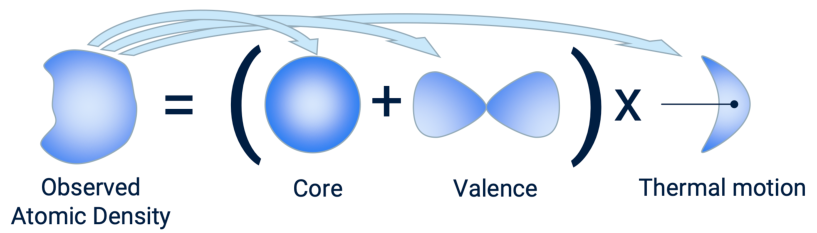
\includegraphics[width=0.6\linewidth]{Figures/valencevsthermaled.pdf}
    \caption[Correlation of thermal and dipolar functions.]{Thermal motion (described by anisotropic displacement parameters) and dipolar basis terms are highly correlated.}\label{fig:adp-dipole}
\end{figure}

For this reason, it is critical to establish accurate atomic positions and ADPs before refining the multipole parameters and charge density.
Traditionally this was done using neutron data which, as mentioned above, is insensitive to electron density perturbations as neutrons are scattered almost exclusively by the nucleus.
Unfortunately neutron sources are notoriously expensive and low-flux, requiring extremely large crystals which introduces further errors due to extinction.
With the advent of modern x-ray diffractometer technology, we can luckily determine atomic coordinates and ADPs using x-ray data alone.
This is done using high angle reflections, which are dominated by core scattering and thus contain little data from the diffuse bonding electron density.
Core electron density is almost perfectly spherical, allowing ADPs to be correctly refined from this data.
With accurate atomic coordinates and ADPs in hand, hydrogen atoms can be located in the low angle data, and then the multipole parameters refined to convergence.
Multipole refinement can benefit enormously from an initial database model, particularly for hydrogen atoms, so it is no surprise that the techniques are often used sequentially.\autocite{Guillot2001,Volkov2006}
The resulting electron density can be used to characterise molecules and predict reactivity, particularly when interpreted within the powerful Quantum Theory of Atoms In Molecules framework of Bader.\autocite{Bader1991}
The obvious attraction of this method is that it is almost entirely experimental.
However, the atom centred multipole functions and their resulting sum, while superficially resembling a wave function, is not antisymmetric and is therefore in violation of the Pauli exclusion principle.
It therefore cannot be used to determine \emph{all} properties of a system.

To summarise, electron density can be measured in a crystal by x-ray diffraction, and various models used to fit it.
The ``gold standard'' would be the derivation of a wave function, but at present this has not been done without the introduction of chemical constraints.
In practise, the most accurate and most informative fitting of electron density to diffraction data is done with a series of atom-centred spherical harmonic functions (the Hansen-Coppens formalism).
The resulting electron density can be used in QTAIM analysis, or used to construct electrostatic potential maps, which can guide chemists in their understanding of molecules in crystals.

\section{Nuclear Magnetic Resonance}
Nuclear magnetic resonance spectroscopy (NMR) is an essential tool for all organic chemists, as it is able to give relatively detailed structural information quickly and cheaply.
It is based on the magnetic moment of certain nuclei, which are usually randomly oriented but spontaneously align in the presence of a strong magnetic field.

\subsection{Solid State NMR}
The chemical shift of a nucleus is not a simple scalar quantity, as solution phase NMR experiments might suggest.
The shielding, and hence the effective magnetic field felt by the nucleus depends on the electronic environment around the nucleus, which is decidedly \emph{an}isotropic, therefore incapable of being expressed as a scalar.
Depending on the orientation of the electron cloud (and other shielding/deshielding influences) around the nucleus with respect to the magnetic field, different chemical shifts will be observed for the same nucleus.
This phenomenon is the chemical shift anisotropy of a nucleus, and it is described mathematically by a second rank tensor, which is geometrically depicted as an ellipsoid.

In a solution phase NMR experiment, rapid and random tumbling of the molecules averages out the anisotropy of each signal, affording a sharp peak at the isotropic chemical shift.
This can be simulated to some degree by magic angle spinning in solid-state experiments, but it is often the case that the chemical shift anisotropy is more interesting that the isotropic shift, so a solid phase NMR experiment is the only way to examine it.

The shape of the chemical shift tensor can provide insight into the electronic environment of a nucleus, with large shielding components often being aligned with electronic features such as bonds or lone pairs.
It is often convenient to define a principal axis system (PAS) for the tensor, consisting of two components which describe the longest and shortest axes of the ellipsoid, and the axis perpendicular to both.
The PAS of the chemical shielding tensor is denoted by the lowercase $ x $, $ y $ and $ z $, and the components of the tensor which are aligned with these axes are labelled $ \sigma_{xx} $, $ \sigma_{yy} $ and $ \sigma_{zz} $.
The laboratory reference frame is denoted by the uppercase $ X $, $ Y $ and $ Z $, with the magnetic field $ B_0 $ being aligned with the $ Z $ axis.
A common method for transforming one coordinate system to another is through the use of Euler angles $ \alpha $, $ \beta $ and $ \gamma $, which define sequential right-handed rotations about the axes of the rotating frame.
As the chemical shielding is necessarily invariant to rotation about $ Z $, we can dispense with the first of these angles $ \alpha $, and simply refer to the latter two as the polar angles $ \beta = \theta $ and $ \gamma = \phi $.
The chemical shielding tensor is thus depicted in \cref{fig:chemical-shielding-tensor}, and this will be the convention used in this work.

\begin{figure}
  \centering
  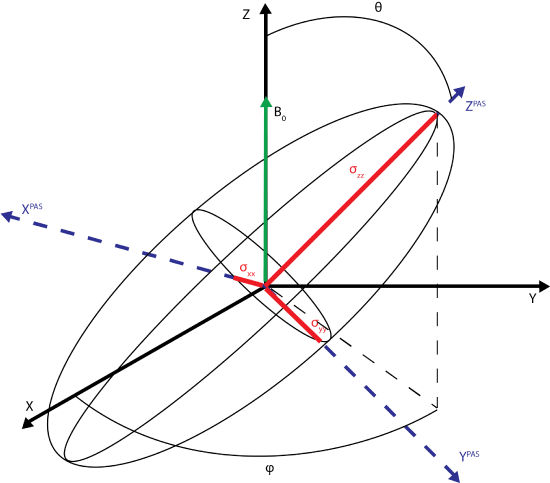
\includegraphics[width=0.4\linewidth]{Figures/Chemical_Shift_Tensor.png}
  \caption[Principal axis system with respect to laboratory reference.]{Representation of the principal axis system (PAS, blue dotted lines) with respect to the laboratory reference frame (black solid lines). The polar angles $ \theta $ and $ \phi $ relate the former to the latter. The principal components of the tensor are shown in red, and the overall shape is shown by the black ellipses.}\label{fig:chemical-shielding-tensor}
\end{figure}

In almost all experiments, the chemical shielding tensor $ \sigma $ is only indirectly measured, via the chemical shift $ \delta $, which is defined with respect to a reference nucleus such that $ \delta = \sigma_{\textrm{ref}} - \sigma_{\textrm{sample}} $.
As the coordinate system as described above is somewhat arbitrary, the IUPAC convention defines the three principal components of the chemical shift tensor $ \delta_{11} $, $ \delta_{22} $ and $ \delta_{33} $ such that $ \delta_{11} \geq \delta_{22} \geq \delta_{33} $.
The isotropic chemical shift is given by the average $ \delta_{\textrm{iso}} = \frac{(\delta_{11} + \delta_{22} + \delta_{33})}{3} $.
There are two other conventions for describing chemical shift anisotropy, which are useful in different contexts.
The Herzfeld Berger convention represents the chemical shift in terms of the span of the signal $ \Omega = \delta_{11} - \delta_{33} $ and the skew $ \kappa = \frac{3(\delta_{22} - \delta_{\textrm{iso}})}{\Omega} $ where $ \delta_{\textrm{iso}} $ is the same as in the IUPAC convention.
This is particularly useful for intuitively describing the powder line shape formed by a given signal.
The other convention is the Haeberlen convention, which defines the three principal components as $ |\delta_{zz} - \delta_{\textrm{iso}}| \geq |\delta_{xx} - \delta_{\textrm{iso}}| \geq |\delta_{yy} - \delta_{\textrm{iso}}| $, and the parameters $ \Delta_{\textrm{CSA}} = \delta_{zz} -\delta_{\textrm{iso}} $ and $ \eta_{\textrm{CSA}} = \frac{\delta_{xx} - \delta_{yy}}{\delta_{zz} -\delta_{\textrm{iso}}} $.
This convention is most useful for describing the angular dependence of a chemical shift on the polar angles $ \theta $ and $ \phi $, which is given by the relationship\autocite{Haeberlen1976}
\begin{equation}
  \delta_{\textrm{obs}} = \delta_{\textrm{iso}} + \Delta_{\textrm{CSA}} \left(\frac{3 \cos^2 \theta - 1 + \eta_{\textrm{CSA}} \sin^2 \theta \cos 2 \phi}{2} \right)
  \label{eqn:orientation-csa}
\end{equation}

In a non-spinning polycrystalline or amorphous powder, the above expression can be integrated over the range of chemical shifts to give the characteristic powder line shape see in \cref{fig:ssnmr-tensor}, reproduced from the work of Facelli, Grant, and Michl.\autocite{Facelli1987Carbon-13Determination}
The sample consists of randomly oriented tensors, all of which contribute to the signal.
The principal values of the tensor $ \delta_{11} $, $ \delta_{22} $ and $ \delta_{33} $ correspond to the two extrema of the line, and the central peak.

\begin{figure}
  \centering
  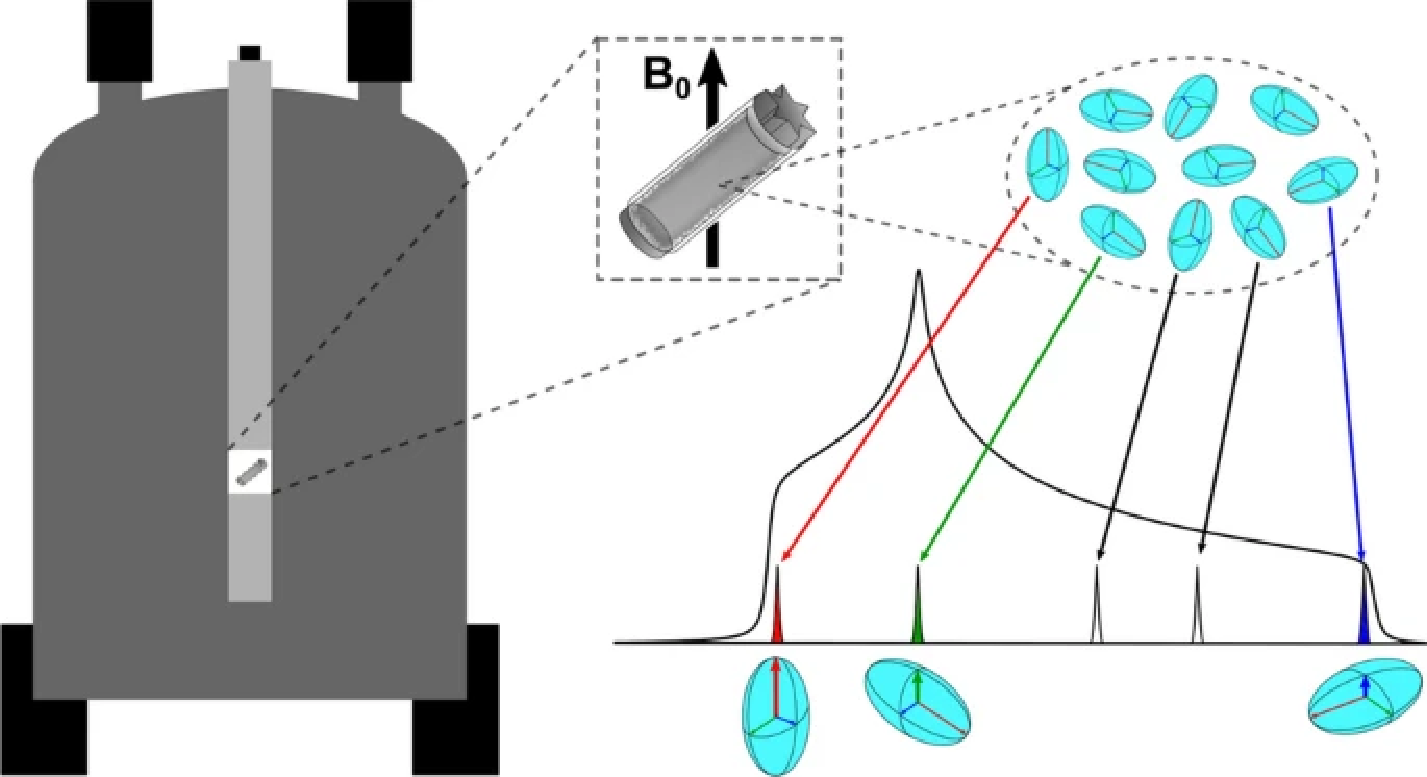
\includegraphics[width=0.45\linewidth]{Figures/ssnmr-tensor.pdf}
  \caption[SS-NMR powder line shape]{Characteristic solid-state NMR powder line shape for an asymmetric tensor e.g.\ in an alkene. The positions of the three principal values are shown.}\label{fig:ssnmr-tensor}
\end{figure}

Spinning at the magic angle can improve the S/N ratio by partially averaging out the chemical shift anisotropy and dipolar relaxation.
Instead of the powder pattern, we instead observe a sharp isotropic chemical shift and a series of spinning sidebands which are separated from the isotropic peak by multiples of the spinning frequency.
The radiated power is thus concentrated in narrower bands, leading to a much improved S/N ratio.

An example is presented in \cref{fig:31P-ssnmr} of proton decoupled solid state \ce{^{31}P} spectra of barium diethyl phosphate, reproduced from the work of Herzfeld and Berger\autocite{Herzfeld1980SidebandAngle}.
In the first spectrum, no magic angle spinning was used, and the line shape is characteristically broadened into an asymmetric peak (the powder line shape).
Note the poor S/N ratio due to the broad peak.
The S/N ratio can be seen to improve as the spinning speed increases, and the sidebands become more sparse, affording a stronger signal overall.

\begin{figure}
    \centering
    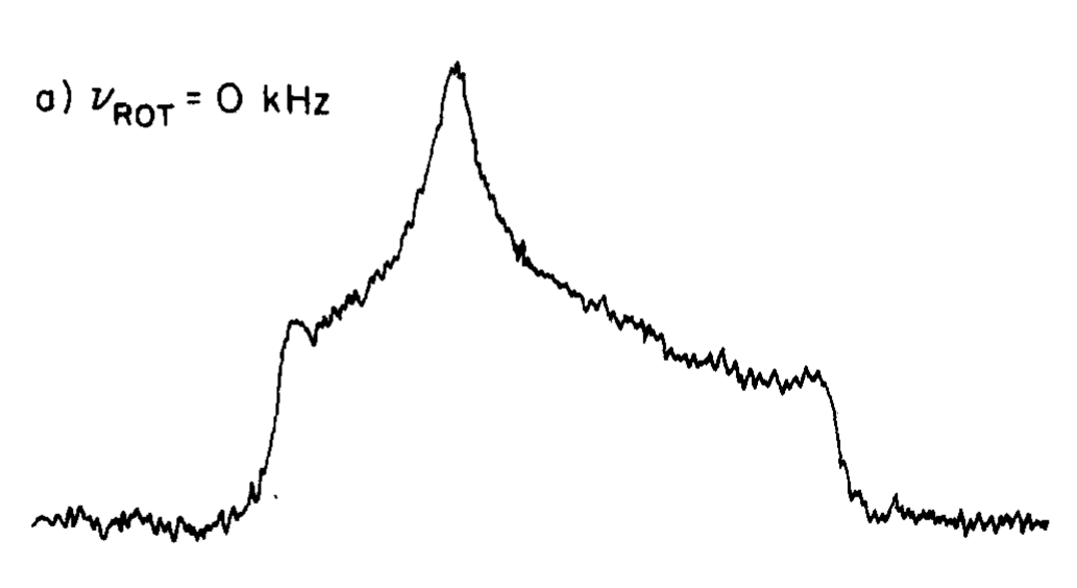
\includegraphics[width=0.45\linewidth]{Figures/31P-ssnmr-0khz.pdf}
    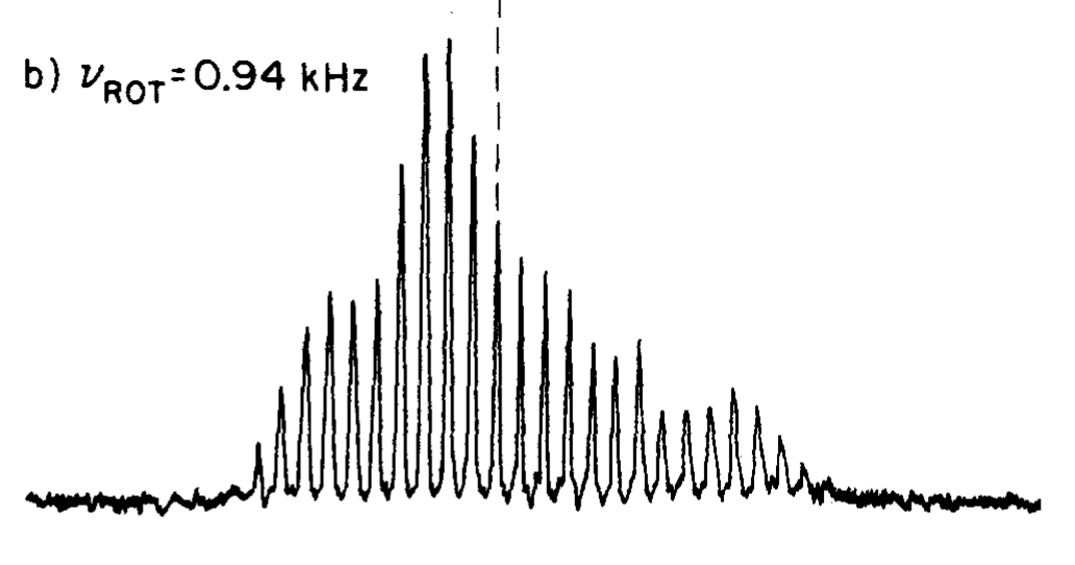
\includegraphics[width=0.45\linewidth]{Figures/31P-ssnmr-0.94khz.pdf}

    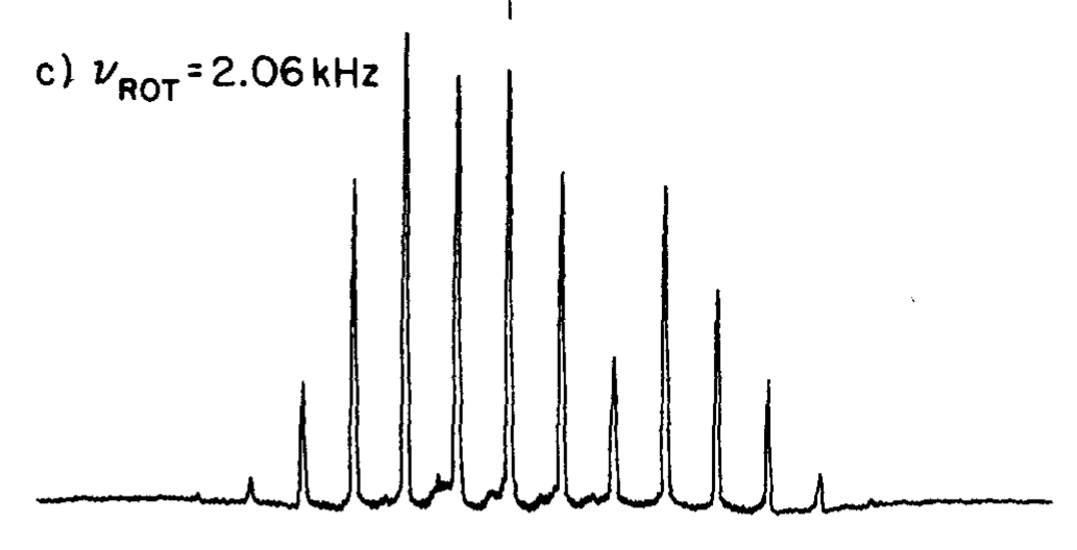
\includegraphics[width=0.45\linewidth]{Figures/31P-ssnmr-2.06khz.pdf}
    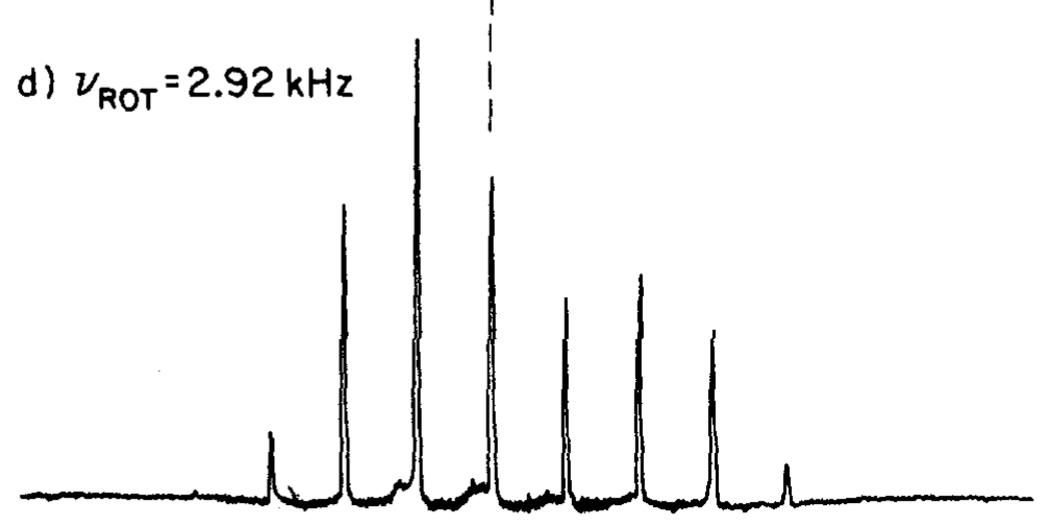
\includegraphics[width=0.45\linewidth]{Figures/31P-ssnmr-2.92khz.pdf}
    \caption[31P SS-NMR spinning at the magic angle.]{Proton decoupled solid state \ce{^{31}P} spectra of barium diethyl phosphate spinning at the magic angle, at the speed specified. The isotropic chemical shift is shown by the vertical dotted line.}\label{fig:31P-ssnmr}
\end{figure}

The principal values of the tensor are clearly easily obtained from a non-spinning sample, as they can practically be read off the spectrum.
However, the extremely poor S/N ratio (especially for a relatively insensitive nucleus like \ce{^{77}Se}) limits the utility of this method.
Spinning at the magic angle is clearly necessary to improve the S/N ratio, however this obscures the true locations of the extrema of the signal, therefore the values of $ \delta_{11} $ and $ \delta_{33} $, as well as modifying the position of the maximum ($ \delta_{22} $).

There exist programs (such as SOLA, integrated within TopSpin by Bruker BioSpin) which can fit an experimental line shape or sideband manifold affording the principal values of the tensor, however there is clearly a trade-off between obtaining a good S/N ratio and having enough sidebands within the limits of the signal for a meaningful fit.
Perhaps the most fundamental issue stems from the fact that the sample is a powder of randomly oriented particles.
This means that the absolute orientation of the tensor with respect to the molecule cannot be determined from this kind of experiment.
Nonetheless, the \emph{shape} of the tensor is still valuable information that may be able to shed light on Ch-bonding in the solid phase.

\printbibliography[heading=subbibliography]
\end{refsection}


\part{The strength and nature of chalcogen bonding}

\begin{refsection}

    \chapter[Insights from co-crystal structures]{New insights into chalcogen bonding provided by co-crystal structures of benzisoselenazolinone derivatives and nitrogen bases}\label{sec:crystengcomm1}
    
    This chapter was published in Cryst.\ Eng.\ Comm., 22 Jan 2019\autocite{Fellowes2019}.\footnote{Compound numbering, section headings, and terminology have been updated to fit this thesis.}
    
    \section{Abstract}
    A number of derivatives of benzisoselenazolinones, including the drug ebselen, have been synthesized, and their interactions with various nitrogen bases characterized through x-ray crystallography.
    Structural studies revealed a strong interaction in all cases, with \ce{Se \cdots N} distances well within the Van der Waals radii of the constituent atoms.
    We suggest that there is a significant charge transfer component to this interaction, in contrast to some other interactions of similar strength and directionality.
    We have also found that this interaction can be enhanced via H-bonding to the carbonyl group of the benzisoselenazolinone moiety.
    
    \cmpd*{ebs}
    \cmpd*{ebs.bn}
    \cmpd*{ebs.h}
    \cmpd*{amide}
    \cmpd*{amide.bn}
    \cmpd*{amide.h}
    \cmpd*{tetracycle}
    
    \section{Introduction}
    Chalcogen bonding (Ch-bonding) is a class of non-covalent interaction which has recently piqued the interests of the chemical community, and potential applications in materials and medicinal chemistry are emerging.\autocite{Mitchell2017,Wonner2017a,Fanfrlik2014,Vogel2019}
    It bears similarities to the related concept of halogen bonding, and the ubiquitous phenomenon of hydrogen bonding, in that the result is a relatively strong and highly directional non-bonded interaction.\autocite{Paolo1974}
    This strength and directionality has been exploited in crystal engineering\autocite{Gleiter2003,Kremer2016,Huynh2017}, anion recognition\autocite{Lim2017,Lim2018,Garrett2016}, and bond activation \autocite{Wonner2017,Benz2017,Benz2017a}, and appears to play a critical role in protein folding.\autocite{Iwaoka2001,Iwaoka2015}
    Studies on \ce{Te \cdots N} Ch-bonds in solution phase have shown they can be as strong as 2.7~kcal/mol\autocite{Garrett2015a}.
    A number of interesting and potentially useful supramolecular polymers have been synthesised and characterised by \citeauthor{Ho2016,Ho2017}, based on tellurium- and selenium-containing heterocycles.\autocite{Ho2016,Ho2017}
    
    In our efforts to apply the concept of Ch-bonding to biological systems, we turned to the benzisoselenazolinone scaffold of the antioxidant compound ebselen \cmpd{ebs}.
    \cmpd{ebs} has been known since the 1980s to effectively scavenge reactive oxygen species \emph{in vivo}.\autocite{Muller1984}
    It has remarkably low toxicity for an organoselenium compound, and is being investigated as a possible treatment for a number of conditions.\autocite{Schewe1995,Kil2007,Singh2013,Parnham2000}
    It is also an ideal scaffold for Ch-bonding, bearing a selenium atom bonded to an electronegative amide nitrogen.
    Indeed, Ch-bonding in \cmpd{ebs} has been investigated previously in the context of crystal packing of the pure compound, but there is a lack of experimental evidence for interactions with other acceptors.\autocite{Thomas2015}
    
    Numerous studies have examined the nature of the Ch-bond, in particular the balance between electrostatic effects (due to anisotropic electrostatic potential around the chalcogen atom), covalent (orbital overlap and electron delocalisation), and dispersion forces.\autocite{Oliveira2017,Pascoe2017,DeVleeschouwer2017,Kolar2016,Gleiter2018}
    In the case of halogen bonding, these contributions are generally well characterized.
    Halogen bonds range from primarily electrostatic (as in the case of fluorinated iodobenzenes\autocite{Prasang2009}) to charge-transfer dominated (molecular halogens\autocite{Mulliken1950}).
    In the case of Ch-bonding in derivatives of \cmpd{ebs}, the contributions are less clear.
    We therefore sought to characterize Ch-bonding interactions between a number of derivatives of \cmpd{ebs}, and a variety of Ch-bond acceptors.
    
    
    \section{Results and Discussion}
    \subsection[Synthesis of \refcmpd{ebs,ebs.bn,tetracycle}]{Synthesis of benzisoselenazolinone derivatives \refcmpd{ebs,ebs.bn,tetracycle}}
    Compounds \cmpd{ebs} and \cmpd{ebs.bn} were synthesized via published procedures from amides \cmpd{amide} and \cmpd{amide.bn}.\autocite{Bhabak2010}
    The Se-tetracycle \cmpd{tetracycle} was isolated in poor yield as the major product from the cyclization of primary amide \cmpd{amide.h} in an attempt to form \cmpd{ebs.h}.
    It is noteworthy that the spectral characteristics of \cmpd{tetracycle} are essentially identical to reported spectral data of \cmpd{ebs.h}\autocite{Bhabak2010}.
    
    \begin{scheme}
      \centering
      \replacecmpd{amide,amide.bn}
      \replacecmpd{ebs,ebs.bn}
      \replacecmpd{amide.h}
      \replacecmpd{ebs.h}
      \replacecmpd{tetracycle}
      \replacecmpd{ebs}
      \replacecmpd{ebs.bn}
      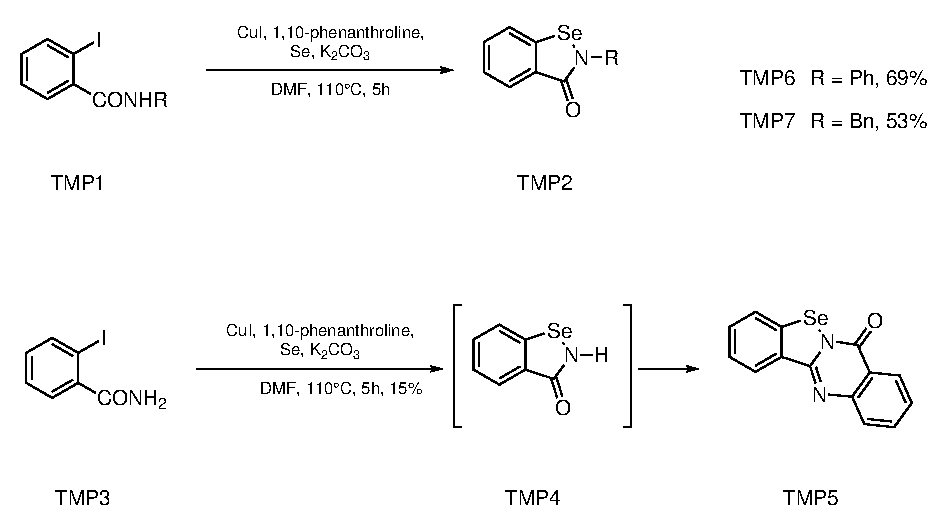
\includegraphics[scale=0.74]{Figures/catalytic-synthesis.eps}
      \caption{Synthesis of Ch-bond donors \refcmpd{ebs}, \refcmpd{ebs.bn} and \refcmpd{tetracycle}.}\label{fig:synthesis}
    \end{scheme}
    
    \begin{table}
      \centering
      \caption{Selected structural parameters of Ch-bonded complexes.}\label{tab:bondlengths}
      \tablefit{\begin{tabular}{lllllll}
        \toprule
        Complex & r(\ce{N \cdots Se}) & r(\ce{Se-N_{1}}) & r(\ce{Se-C_{1}}) & r(\ce{N-C(O)}) & $ \angle $(\ce{N \cdots Se-N_{1}}) & $ \angle $(\ce{C_{para} \cdots N \cdots Se}) \\
          & \AA\ & \AA\ & \AA\ & \AA\ & \degree\ & \degree\  \\ \midrule
        \cmpd{ebs} only & --- \\
        \cmpd{ebs} $ \cdot $ DMAP & 2.371(1) & 1.9676(10) & 1.8959(12) & 1.2345(14) & 174.18(4) & 173.52(4) \\
        \cmpd{ebs.bn} only & --- & 1.8805(14) & 1.8867(16) & 1.350(2) & --- & --- \\
        \cmpd{ebs.bn} $ \cdot $ DMAP M1 & 2.4276(14) & 1.9297(13) & 1.8984(15) & 1.348(2) & 173.93(5) & 174.89(5) \\
        \cmpd{ebs.bn} $ \cdot $ DMAP M2 & 2.4331(14) & 1.9191(14) & 1.8966(14) & 1.349(2) & 175.30(5) & 158.14(5) \\
        \cmpd{ebs.bn} $ \cdot $ DMAP $ \cdot $ \ce{H2O} & 2.4046(15) & 1.9367(14) & 1.9070(14) & 1.330(2) & 175.54(5) & 167.43(5) \\
        \cmpd{ebs.bn} $ \cdot $ quinuclidine & 2.5874(17) & 1.9077(17) & 1.898(2) & 1.354(3) & 176.77(7) & 161.32(7) \\
        \cmpd{ebs.bn} $ \cdot $ DABCO & 2.6166(15) & 1.9019(14) & 1.8967(17) & 1.355(2) & 175.76(6) & 160.00(6) \\
        \cmpd{tetracycle} only & --- & 1.883(2) & 1.899(3) & 1.393(3) & --- & --- \\
        \cmpd{tetracycle} $ \cdot $ pyridine & 2.461(3) & 1.926(2) & 1.908(3) & 1.373(4) & 174.13(9) & 169.1(1)\\
        \cmpd{tetracycle} $ \cdot $ DMAP & 2.304(1) & 1.9716(9) & 1.918(1) & 1.375(1) & 173.81(4) & 173.16(4) \\
        \bottomrule
        \end{tabular}}
    \end{table}
    
    \subsection{Co-crystal structures of benzisoselenazolinones and Lewis bases}
    High quality low temperature crystal structures were obtained for the parent benzisoselenazolinone derivatives \cmpd{ebs} \autocite{Thomas2015}, \cmpd{ebs.bn} and the Se-tetracycle \cmpd{tetracycle} and the chalcogen-bonded co-crystals of these compounds with a variety of nitrogen bases, including pyridine, dimethylaminopyridine (DMAP), quinuclidine and 1,4-diaza\-bicyclo[2.2.2]\-octane (DABCO).
    Powder diffraction patterns were obtained of the bulk co-crystal material and compared with the single crystal data, with excellent agreement.
    This provides strong evidence of phase purity, with the exception of \cmpd{ebs.bn}$ \cdot $DMAP, which indicated the presence of the unbound monomers in addition to the Ch-bonded adduct.
    Relevant structural parameters are presented in \cref{tab:bondlengths}, while all thermal ellipsoid plots are presented in the supplementary material (\cref{sec:ch3-si}).
    In the following discussion we begin by assessing the Ch-bond donor abilities of \cmpd{ebs}, \cmpd{ebs.bn}, and \cmpd{tetracycle} by comparing the structural parameters with a common nitrogen base adduct (DMAP), followed by comparison of a single Ch-bond donor \cmpd{tetracycle} with two different nitrogen bases with markedly different basicities (pyridine and DMAP).
    
    \subsection{Effects of the benzisoselenazolinone on Ch-bond strength}
    The DMAP adducts of \cmpd{ebs}, \cmpd{ebs.bn} and \cmpd{tetracycle} are characterized by near linear \ce{N \cdots Se-N(CO)} angles (\cref{tab:bondlengths}) with \ce{N_{DMAP} \cdots Se}distances which are 2.4276(14) and 2.4331(16)~\AA\ for the two independent molecules of \cmpd{ebs.bn}, 2.371(1)~\AA\ for \cmpd{ebs}, and the strikingly short \ce{N \cdots Se} distance of 2.304(1)~\AA\ for \cmpd{tetracycle}.
    All are well within the van der Waals radii of N and Se of 3.85~\AA\ \autocite{Batsanov2001}.
    The antipodal \ce{Se-N_{1}} bond distance within these adducts is significantly lengthened compared to the free Ch-bond donors, 0.063~\AA\ in \cmpd{ebs}, 0.049~\AA\ in \cmpd{ebs.bn}, and 0.088~\AA\ in \cmpd{tetracycle}, with the degree of lengthening being related in an inverse sense to the \ce{N_{DMAP} \cdots Se}distance, in all cases the (non-antipodal) \ce{Se-C_{1}} bond is essentially unchanged.
    These structural parameters suggest an order of Ch-bond donor abilities \cmpd{ebs.bn} < \cmpd{ebs} < \cmpd{tetracycle}, which is supported by theoretical calculations which are discussed below, as well as being consistent with the \textsuperscript{77}Se NMR chemical shifts.
    
    \subsection{Endocyclic bond lengthening associated with stronger complexes}
    Further discussion is warranted on the \cmpd{ebs.bn}$ \cdot $DMAP adduct.
    Firstly, the two independent molecules of \cmpd{ebs.bn}$ \cdot $DMAP differ significantly with respect to the direction that the nitrogen base lone pair makes with the \ce{Se-N_{1}} bond.
    In molecule 1 this angle is close to collinear at 174.89(5)\degree\ while in molecule 2, this deviates significantly from linearity 158.14(5)\degree.
    Associated with this difference is a slightly longer \ce{N_{DMAP} \cdots Se} distance of 2.4331(14)~\AA\ in molecule 2 compared to 2.4276(14)~\AA\ in molecule 1 ($ \Delta $=0.0055~\AA{}; 3$ \sigma $) and a shorter \ce{Se-N_{1}} distance 1.9191(14)~\AA\ vs 1.9297(14)~\AA\ ($ \Delta $=-0.10~\AA{}; 7.5$ \sigma $) indicating a slightly weaker interaction.
    This can be seen in \cref{fig:benzyl-dmap-xray-2}.
    
    \begin{figure}
      \centering
      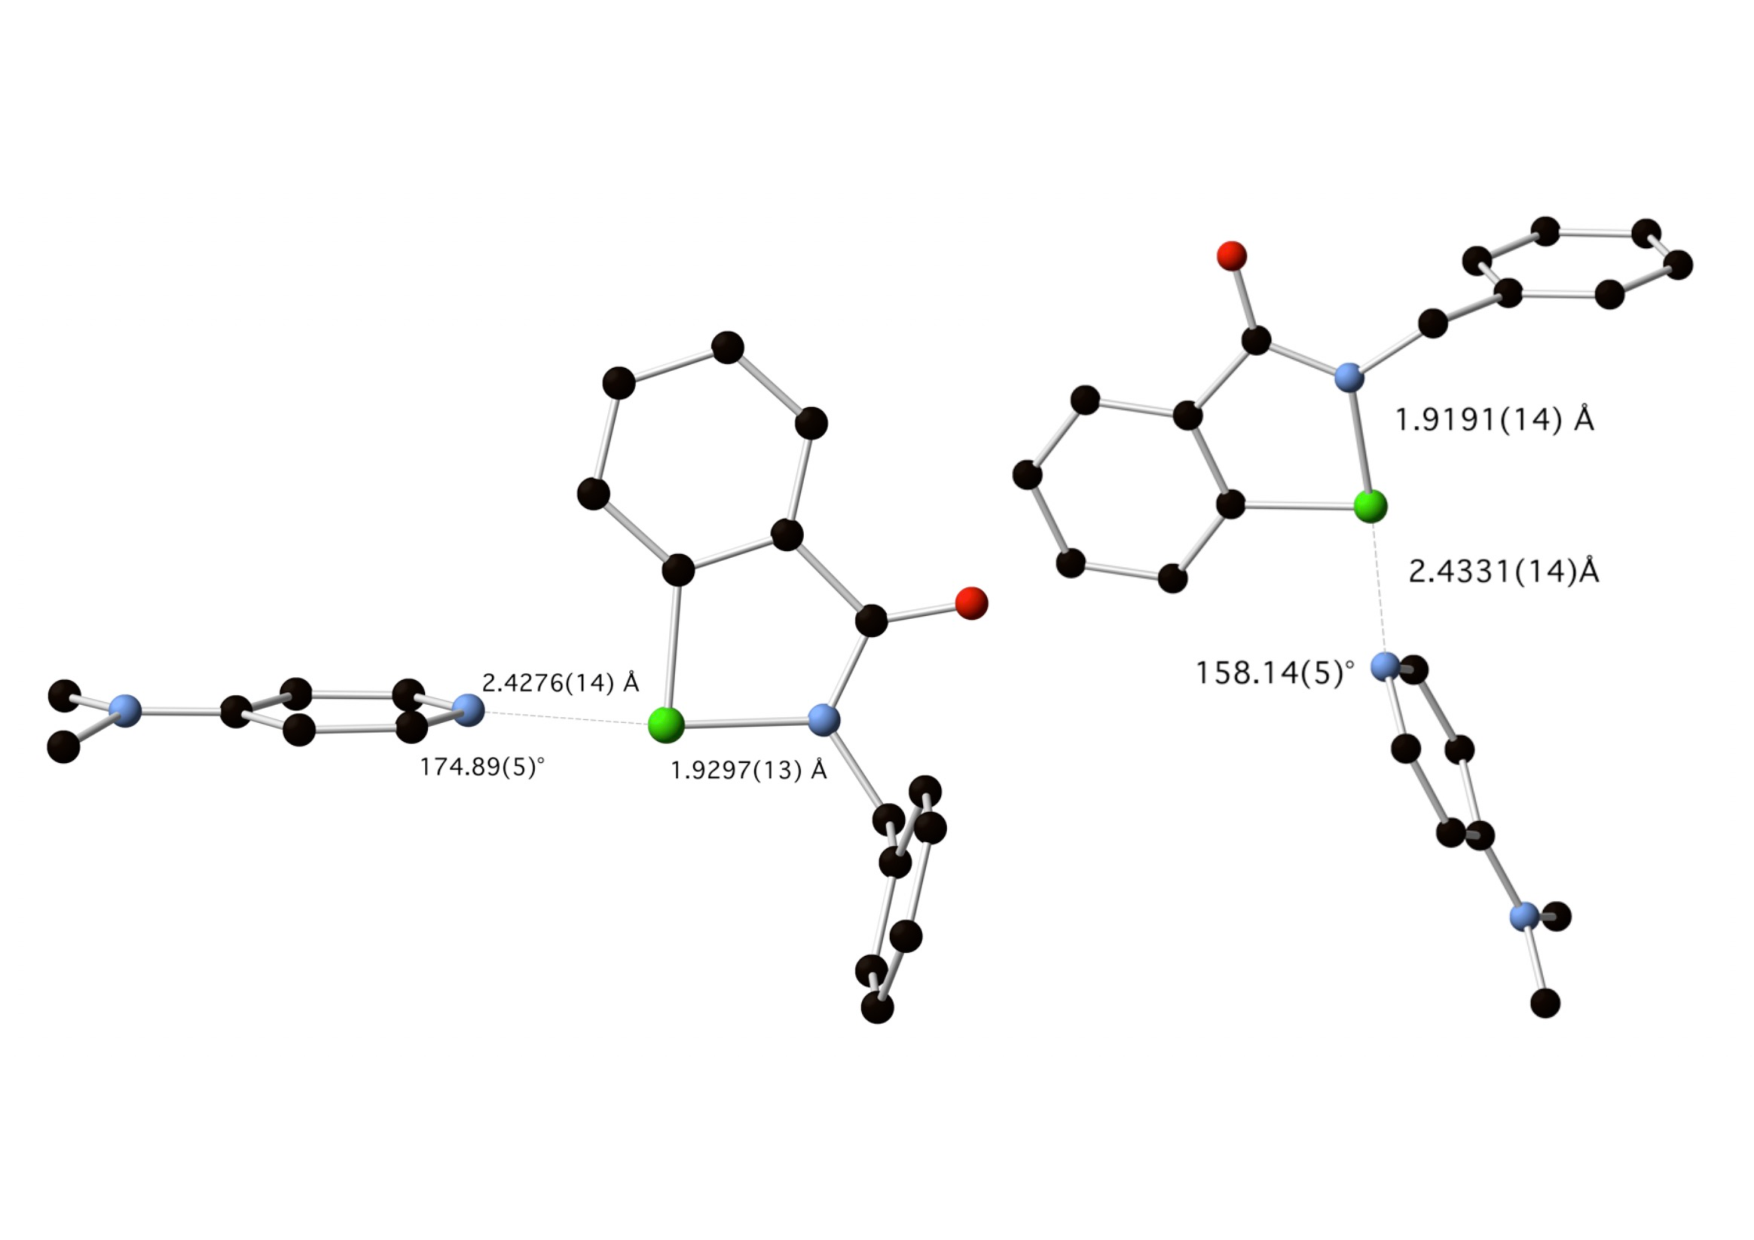
\includegraphics[width=0.8\linewidth]{Figures/benzyl-dmap-xray-2.pdf}
      \caption{Structure of \refcmpd{ebs.bn}$ \cdot $DMAP, showing the two distinct geometries.}\label{fig:benzyl-dmap-xray-2}
    \end{figure}
    
    The structural effects described, particularly the lengthening of the \ce{Se-N_{1}} bond are consistent with donation of electron density from the nitrogen lone pair into the \ce{Se-N_{1}} anti-bonding orbital being a significant component of these \ce{N \cdots Se} Ch-bonds, which has been described before\autocite{Pascoe2017}.
    
    \subsection{H-bond enhanced Ch-bonding}
    The second reason for further discussion of the \cmpd{ebs.bn}$ \cdot $DMAP adduct is based on the structural parameters obtained for the hydrate structure \cmpd{ebs.bn}$ \cdot $DMAP$ \cdot $\ce{H2O} which was serendipitously obtained by evaporation of a THF solution in an open flask.
    The structure is shown in \cref{fig:benzyl-dmap-hydrate}.
    
    \begin{figure}
      \centering
      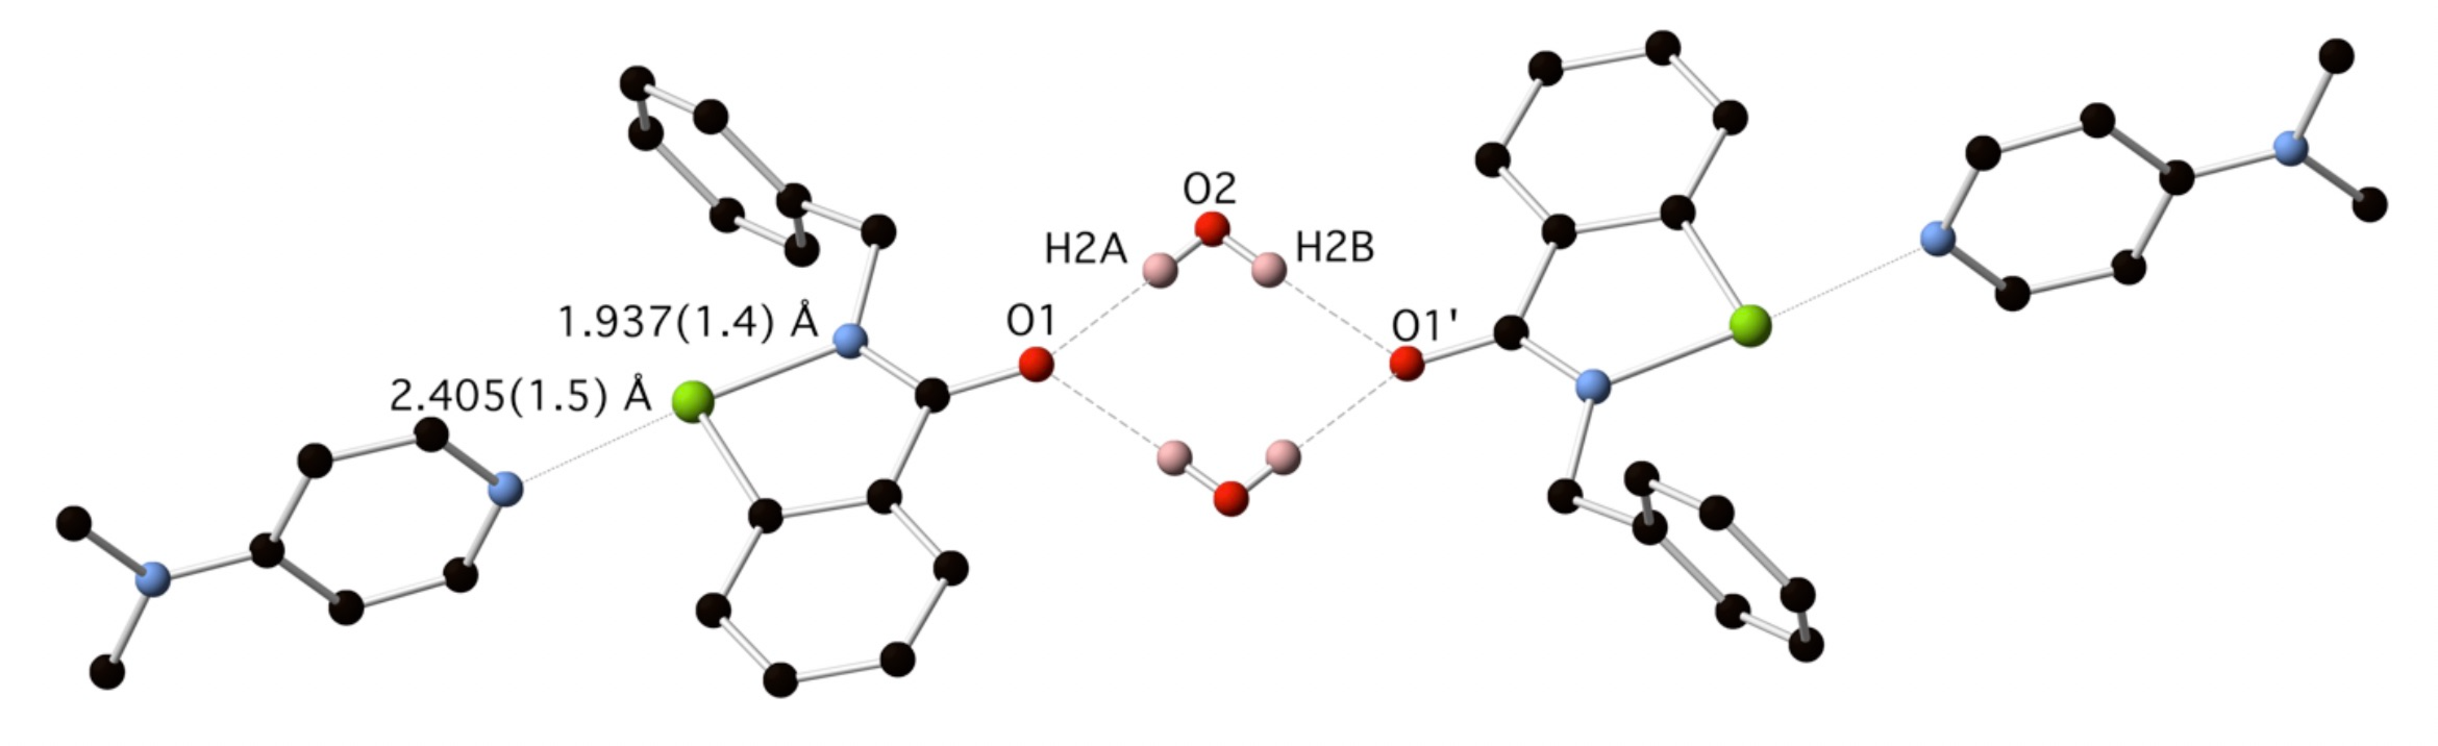
\includegraphics[width=0.8\linewidth]{Figures/benzyl-dmap-hydrate.pdf}
      \caption{Structure of \refcmpd{ebs.bn}$ \cdot $DMAP$ \cdot $\ce{H2O}.}\label{fig:benzyl-dmap-hydrate}
    \end{figure}
    
    \cmpd{ebs.bn}$ \cdot $DMAP$ \cdot $\ce{H2O} crystallizes as a centrosymmetric hydrogen-bonded dimer in which two water molecules bridge two molecules of \cmpd{ebs.bn} across a crystallographic inversion centre.
    Of note, when comparison is made between the structural parameters for \cmpd{ebs.bn}$ \cdot $DMAP molecule 1, which has a similar geometry about the \ce{N \cdots Se} moiety as for \cmpd{ebs.bn}$ \cdot $DMAP$ \cdot $\ce{H2O}, there is a significant contraction of the \ce{N_{DMAP} \cdots Se}distance from 2.4276(14)~\AA\ to 2.4046(14)~\AA\ ($ \Delta $=-0.023~\AA{}; 16$ \sigma $), and an increase in the \ce{Se-N_{1}} bond distance from 1.9297(13) to 1.9367(14)~\AA\ ($ \Delta $=0.007~\AA{}; 5$ \sigma $).
    We have coined the term `hydrogen-bond enhanced Ch-bonding' to describe this interesting structural effect.
    
    \subsection{Effects of the Lewis base on Ch-bond strength}
    We were fortunate to obtain crystal structures of the Se-tetracycle \cmpd{tetracycle} with both pyridine and DMAP, which gave us the opportunity to compare the structural effects arising from two Ch-bond acceptors with significantly different basicities.
    The pyridine adduct of \cmpd{tetracycle} is characterized by a \ce{N_{PYR} \cdots Se} distance 2.461(3)~\AA\ and \ce{Se-N_{1}} distance of 1.926(2)~\AA\ and a near linear \ce{N_{PYR} \cdots Se-N_{1}} angle, the \ce{Se-N_{1}} bond distance is significantly longer than the corresponding distance 1.883(2)~\AA\ in non-bound structure of \cmpd{tetracycle}.
    The DMAP adduct of \cmpd{tetracycle} is characterized by a significantly shorter \ce{N_{DMAP} \cdots Se} distance of 2.304(1)~\AA\ ($ \Delta $=-0.157~\AA) and longer \ce{Se-N_{1}} distance of 1.9716(9)~\AA\ ($ \Delta $=0.046~\AA), consistent with a significantly stronger interaction.
    
    \begin{figure}
      \centering
      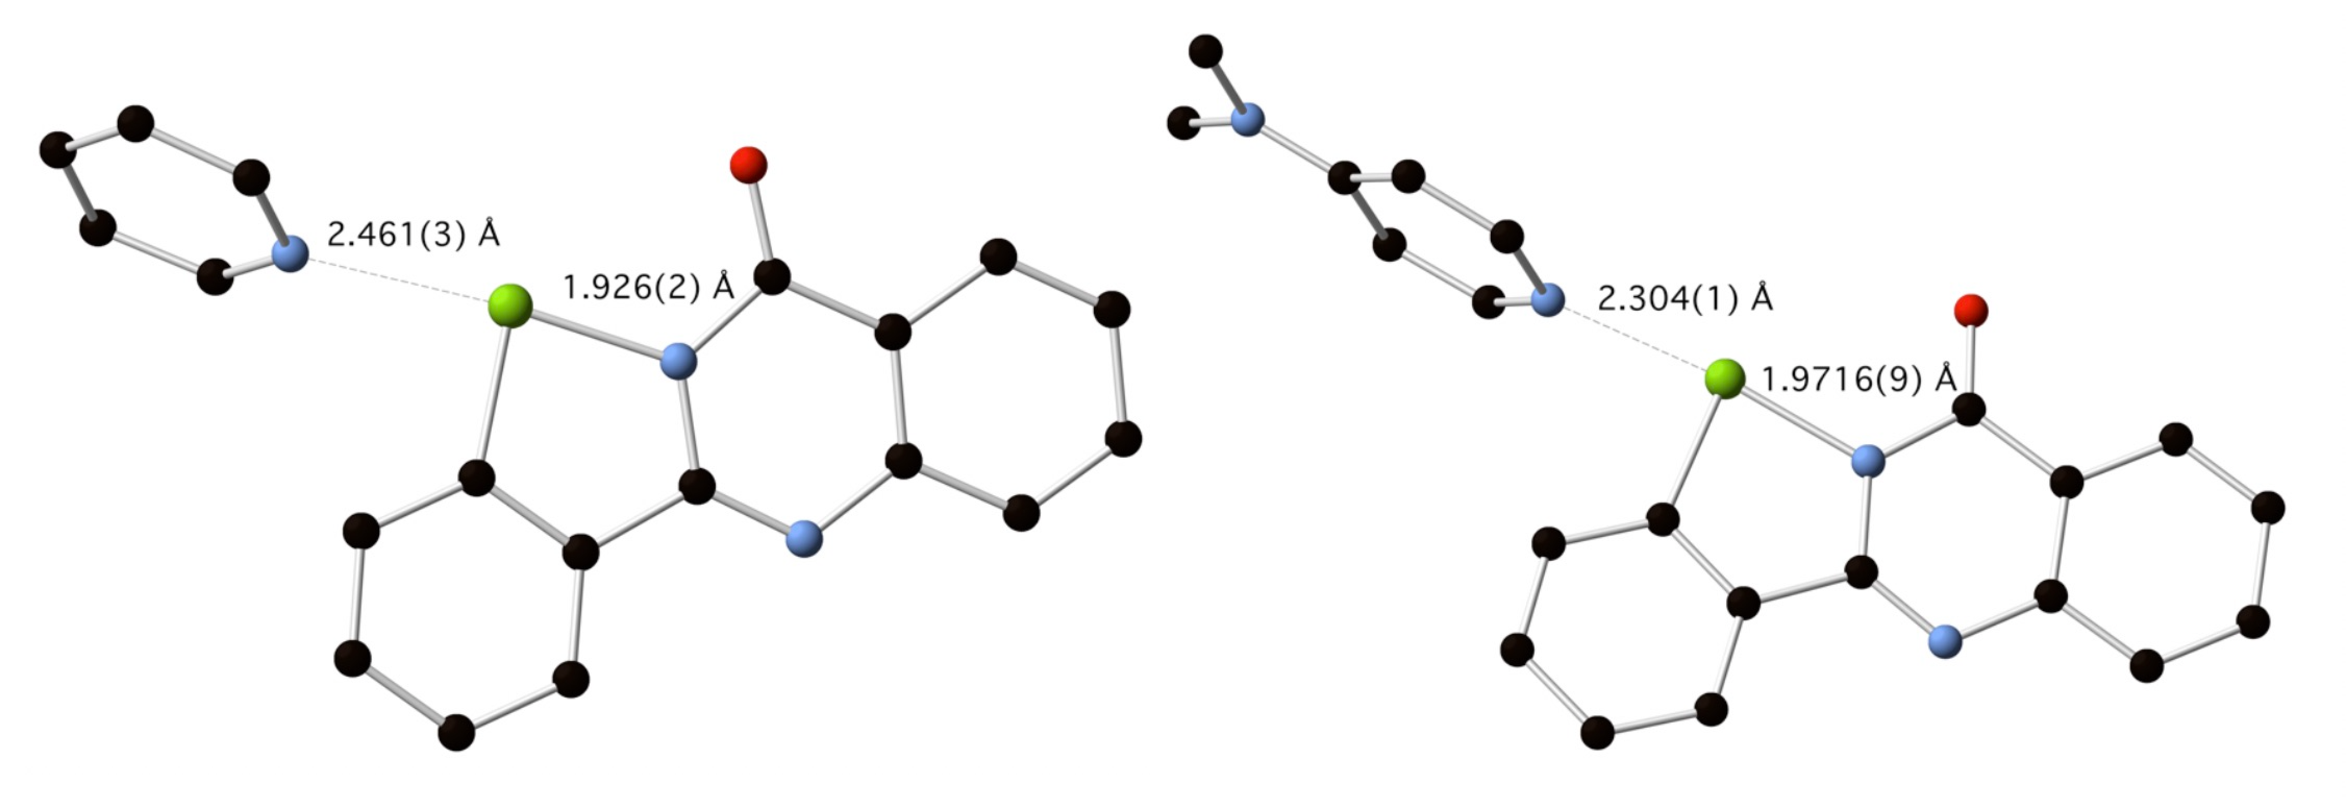
\includegraphics[width=0.8\linewidth]{Figures/dimer-dmap-py-xray.pdf}
      \caption{Pyridine and DMAP adducts of Se-tetracycle \refcmpd{tetracycle}.}\label{fig:dimer-adducts}
    \end{figure}
    
    Ch-bonded co-crystals of the benzisoselenazolinone derivative \cmpd{ebs.bn} with the tertiary amines; quinuclidine and DABCO were obtained and structurally characterized.
    The adducts are presented in \cref{fig:benzyl-adducts}.
    The \ce{N_{QUIN} \cdots Se} and \ce{N_{DABCO} \cdots Se} distances of 2.5874(17)~\AA\ and 2.6166(15)~\AA\ for \cmpd{ebs.bn}$ \cdot $quinuclidine and \cmpd{ebs.bn}$ \cdot $DABCO respectively are significantly longer than those observed for \cmpd{ebs.bn}$ \cdot $DMAP suggesting an order of Ch-bond strengths with \cmpd{ebs.bn} DABCO < Quinuclidine < DMAP which correlates well with the hydrogen bond acceptor ability of these bases, as quantified by the pK\textsubscript{HB} (\cref{tab:pkhb}).
    
    \begin{table}
      \centering
      \caption{Hydrogen bond basicities of bases studied.}\label{tab:pkhb}
      \begin{tabular}{lllll}
        \toprule
                                & pyridine                      & DABCO                     & quinuclidine              & DMAP \\\midrule
          pK\textsubscript{HB}  & 1.86\autocite{Berthelot1998}  & 2.63\autocite{Graton2002} & 2.71\autocite{Graton2002} & 2.80\autocite{Berthelot1998}\\
          \cmpd{ebs.bn}$ \cdot $base r(\ce{N \cdots Se}) / \AA\ & ---   & 2.6166(15)                & 2.5874(17)                & 2.4276(14)\footnote{Bond distance given is the shorter of the two coordination environments.}\\
          \cmpd{ebs.bn}$ \cdot $base $ \Delta $H\textsubscript{f} / kcal/mol & -6.35    & -7.82 & ---                       & -7.91\\\bottomrule
      \end{tabular}
    \end{table}
    
    \begin{figure}
      \centering
      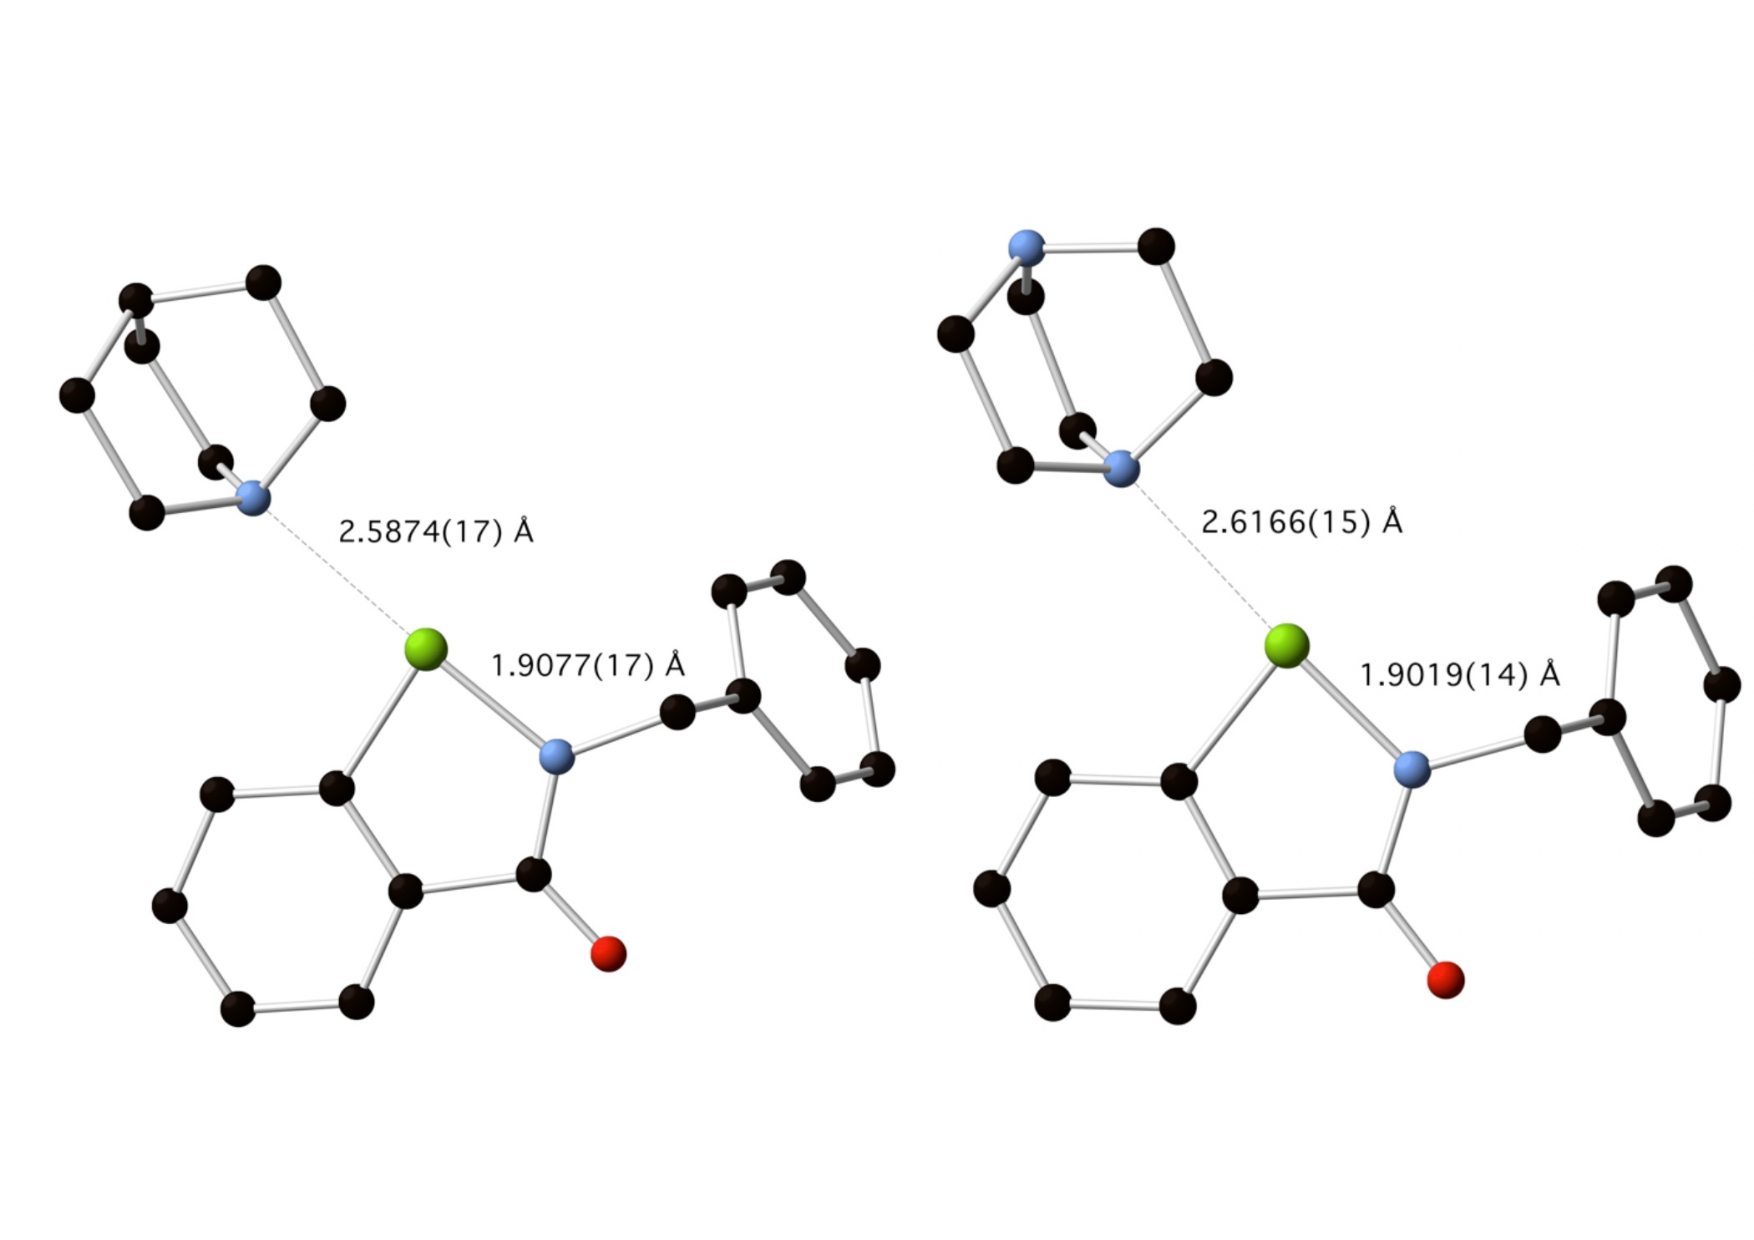
\includegraphics[width=0.8\linewidth]{Figures/benzyl-quin-dabco-xray.pdf}
      \caption{Adducts of benzisoselenazolinone \refcmpd{ebs.bn} with quinuclidine and DABCO.}\label{fig:benzyl-adducts}
    \end{figure}
    
    \subsection{DFT interaction energies and NBO analysis}
    Interaction energies for the complexes were calculated using the $ \omega $B97X-D dispersion corrected functional, which has been used to study similar systems with good agreement with coupled cluster methods.\autocite{Oliveira2017}
    All geometries were therefore optimized at $ \omega $B97X-D/def2-TZVP, and minima verified by frequency analysis.
    
    \begin{figure}
      \centering
      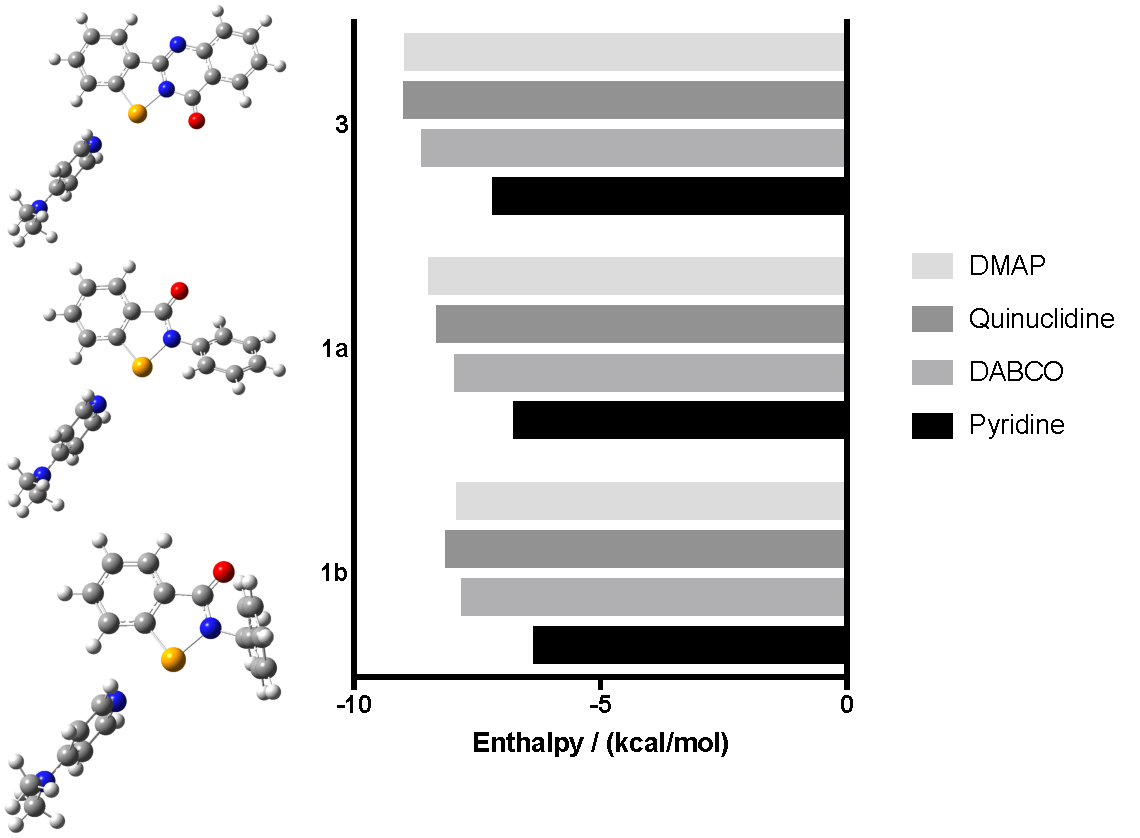
\includegraphics[width=0.8\linewidth]{Figures/dft-energies.pdf}
      \caption[Interaction energies for various complexes.]{Interaction enthalpies calculated at $ \omega $B97X-D/def2-TZVP.\@ Optimised geometries for the DMAP complexes are shown to the left.}
    \end{figure}
    
    NBO analysis was conducted on the optimized geometries, which supports our suggestion that there is a strong orbital component to Ch-bonding in these systems.
    Second order perturbation theory revealed that the energy associated with n(N\textsubscript{base})$ \rightarrow $ $ \sigma^{\star} $(N\textsubscript{1}--Se) delocalisation was 12.79, 15.45, and 16.23~kcal/mol for \cmpd{ebs.bn}$ \cdot $DMAP, \cmpd{ebs}$ \cdot $DMAP, and \cmpd{tetracycle}$ \cdot $DMAP respectively.
    %In the case of the \cmpd{ebs.bn}$ \cdot $DMAP$ \cdot $\ce{H2O} complex, the delocalisation energy was 13.51~kcal/mol.
    %This consistent with our experimental observation of hydrogen-bond enhanced Ch-bonding.
    
    \begin{figure}
      \centering
      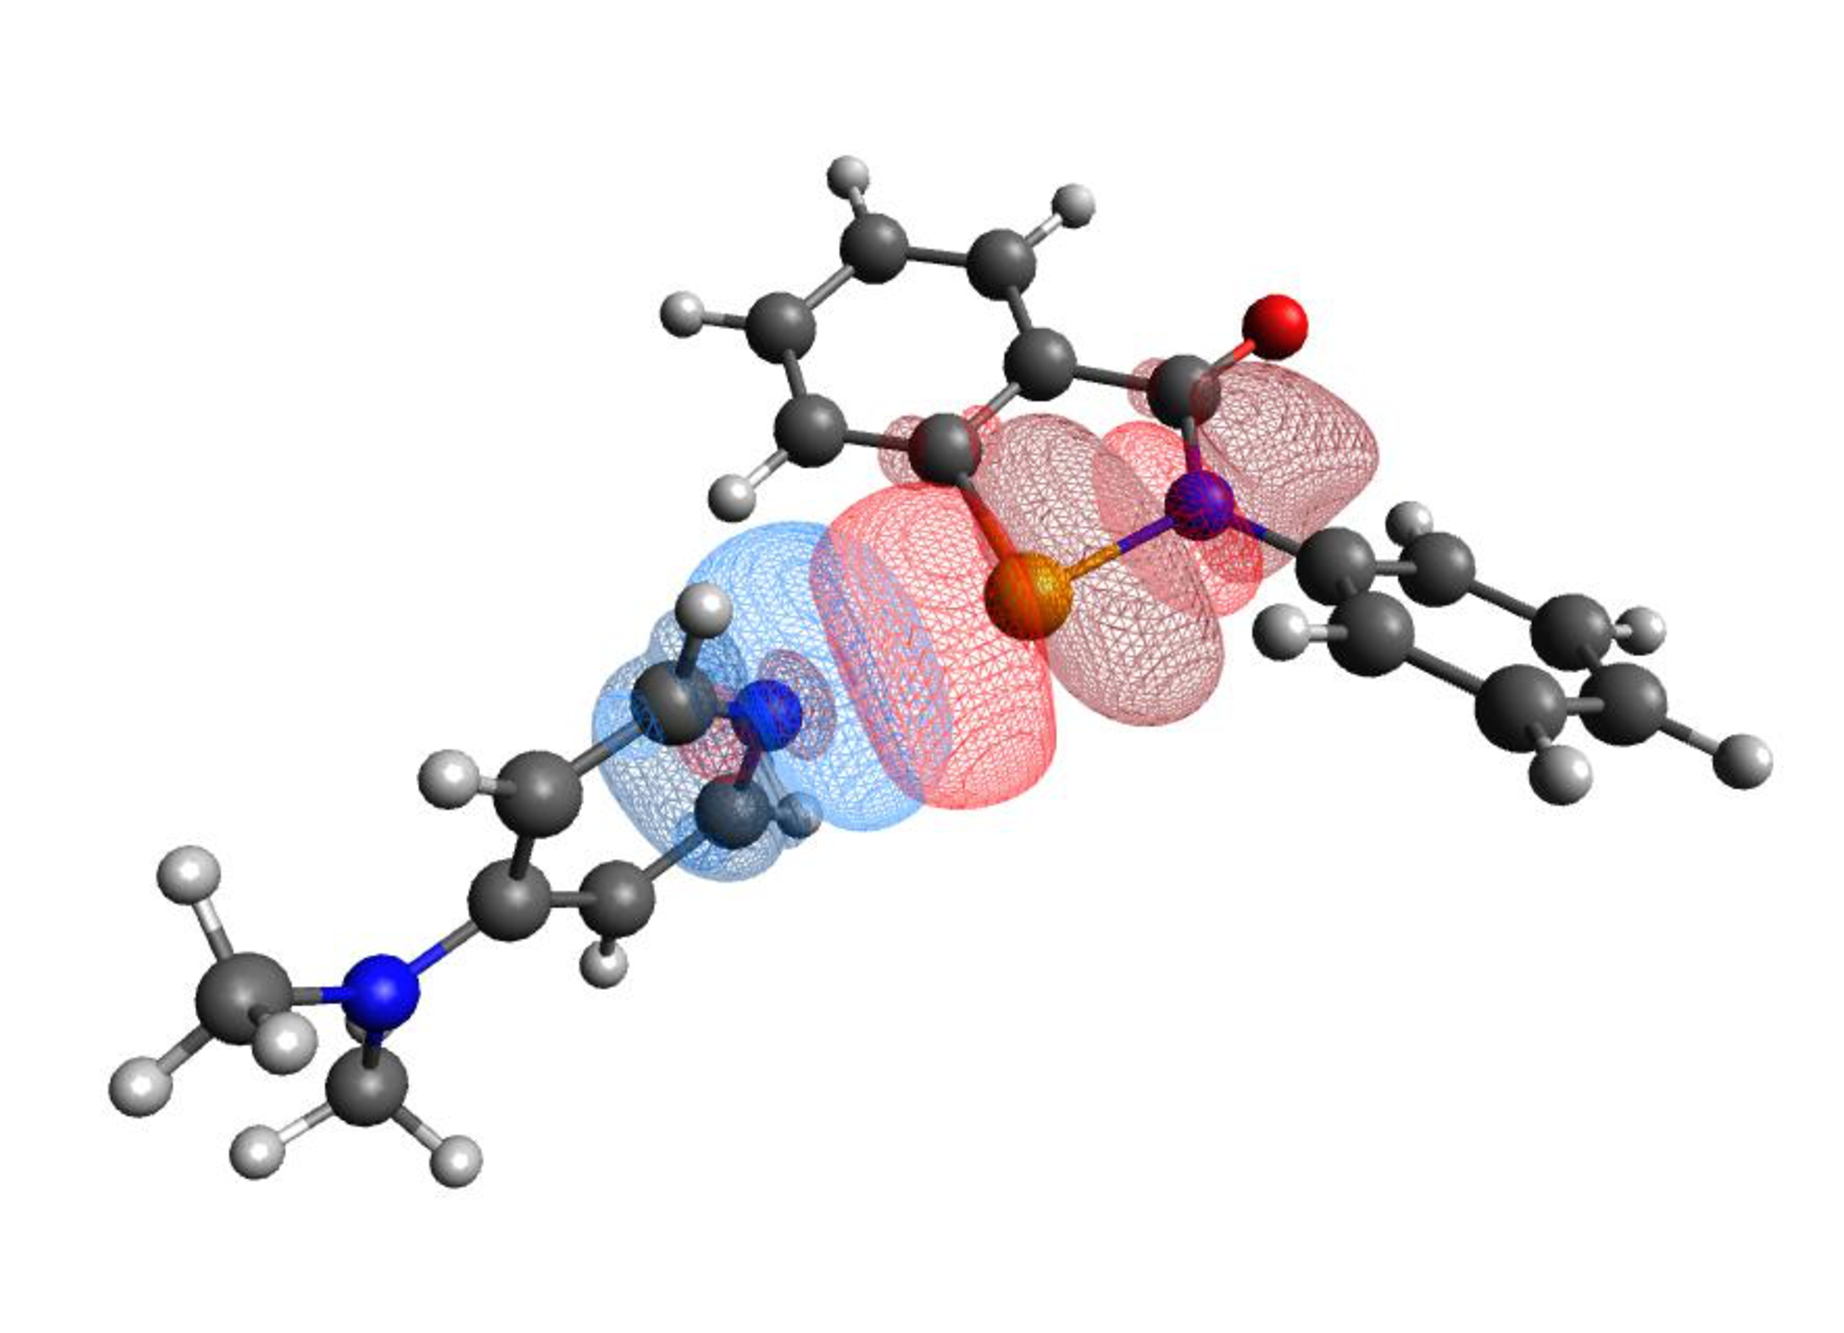
\includegraphics[width=0.6\linewidth]{Figures/phenyl-dmap-overlap.pdf}
      \caption[Orbital overlap for \refcmpd{ebs}$ \cdot $DMAP.]{Overlap of nitrogen lone pair with $ \sigma^{\star} $(\ce{Se-N}) in \refcmpd{ebs}$ \cdot $DMAP complex.}\label{fig:phenyl-dmap-overlap}
    \end{figure}
    
    \section{Conclusion}
    In summary, we have demonstrated the importance of Ch-bonding between derivatives of ebselen \cmpd{ebs} and a variety of nitrogen bases.
    These selenium-containing heterocycles form close contacts with electron pair donors, well within the Van der Waals radii, with predictable geometries consistent with the Ch-bonding model.
    These interactions appear to be primarily due to orbital overlap as opposed to electrostatic or dispersion mediated effects, as evidenced by lengthening of the antipodal \ce{Se-N} bond, and computational analysis, which is consistent with findings in related systems by \citeauthor{Pascoe2017}.\autocite{Pascoe2017}
    We have also found that the strength of a Ch-bond can be enhanced via a hydrogen bond to the carbonyl group of the heterocycle.
    We hope to exploit the strength and directionality of Ch-bonds in ebselen to target biomolecules such as nucleic acids and proteins using compounds containing the isoselenazolinone moiety.
    
    \section{Supplementary materials}
    
    \subsection{Synthetic procedures}
    
    \subsubsection[Preparation of \refcmpd{ebs}.]{Preparation of 2-phenylbenzo[\textit{d}][1,2]selenazol-3(2\textit{H})-one \refcmpd{ebs}.}
    
    Copper iodide (98.4~mg, 0.517~mmol) and 1,10-phenanthroline (83.1~mg, 0.461~mmol) were stirred in anhydrous DMF (3~mL) for 15 mins at r.t., then 2-iodo-N-phenylbenz\-amide (653.2~mg, 2.021~mmol), selenium (196.9~mg, 2.495~mmol) and potassium carbonate (627.3~mg, 4.539~mmol) were added sequentially under a flow of argon.
    The mixture was heated at 110\degree{}C for 8~h, when TLC showed consumption of starting material.
    The mixture was then tipped into brine (30~mL) and stirred to form a brown precipitate, which was extracted into DCM (40~mL) and washed with water ($ 2 \times 20 $~mL).
    The DCM solution was filtered through a silica plug, then evaporated, and the residue applied to a SNAP 25~g silica cartridge, eluting with a petroleum ether/ethyl acetate gradient.
    The major peak was evaporated to afford colourless crystals of \cmpd{ebs} (378.8~mg, 69\%, m.p. 179.1--180.3\degree{}C, lit.\ mp 180--181\degree{}C). 
    
    \ce{^{1}H} NMR (499~MHz, \ce{\textit{d}6}-DMSO) $ \delta $ ppm 8.07 (1H, d, \textit{J} = 8.02~Hz), 7.90 (1H, d, \textit{J} = 7.45~Hz), 7.68 (1H, t, \textit{J} = 7.25~Hz), 7.61 (2H, d, \textit{J} = 7.68~Hz), 7.52--7.42 (3H, m), 7.26 (1H, t, \textit{J} = 7.39~Hz).
    
    \ce{^{77}Se} NMR (95~MHz, \ce{\textit{d}6}-DMSO) $ \delta $ 959.66.
    
    \subsubsection[Preparation of \refcmpd{ebs.bn}.]{Preparation of 2-benzylbenzo[\textit{d}][1,2]selenazol-3(2\textit{H})-one \refcmpd{ebs.bn}.}
    
    Copper iodide (95.8~mg, 0.503~mmol) and 1,10-phenanthroline (93.8~mg, 0.521~mmol) were stirred in anhydrous DMF (3~mL) for 15 mins at r.t., then N-benzyl-2-iodobenz\-amide (860.9~mg, 2.553~mmol), selenium (256.6~mg, 3.249~mmol) and potassium carbonate (542.2~mg, 3.923~mmol) were added sequentially under a flow of argon.
    The mixture was heated at 110\degree{}C for 5~h, when TLC showed consumption of starting material.
    The mixture was then tipped into brine (30~mL) and stirred to form a solid mass, which was dissolved in DCM (40~mL) and washed with water ($ 2 \times 20 $~mL).
    The DCM solution was filtered through a silica plug, then evaporated, and the residue applied to a SNAP 50~g silica cartridge, eluting with a petroleum ether/ethyl acetate gradient.
    The major peak was evaporated to afford pale yellow crystals of \cmpd{ebs.bn} (396.4~mg, 53\%, m.p. 137.8--138.8\degree{}C).
    
    \ce{^{1}H} NMR (400~MHz, \ce{\textit{d}6}-DMSO) $\delta$ ppm 7.99 (1H, d, \textit{J} = 8.04~Hz), 7.83 (1H, d, \textit{J} = 7.7~Hz), 7.59 (1H, t, \textit{J} = 7.56~Hz), 7.42 (1H, t, \textit{J} = 7.44~Hz), 7.37--7.22 (5H, m), 4.9 (2H, s).
    
    \ce{^{77}Se} NMR (95~MHz, \ce{\textit{d}6}-DMSO) $ \delta $ 884.02.
    
    \subsubsection[Preparation of \refcmpd{tetracycle}.]{Preparation of 5\textit{H}-benzo[4,5][1,2]selenazolo[2,3-\textit{a}]quinazolin-5-one \refcmpd{tetracycle}.}
    
    Copper iodide (96.4~mg, 0.503~mmol) and 1,10-phenanthroline (85.7~mg, 0.476~mmol) were stirred in anhydrous DMF (4~mL) for 10~mins at r.t., then 2-iodobenzamide (510.6~mg, 2.067~mmol), selenium (209.5~mg, 2.653~mmol) and potassium carbonate (506.3~mg, 3.663~mmol) were added sequentially under a flow of argon.
    The mixture was heated at 110\degree{}C for 12~h, when TLC showed consumption of starting material.
    The mixture was then tipped into brine (30~mL) and stirred to form a solid mass, which was extracted into ethyl acetate (20~mL) and washed with water ($ 2 \times 20 $~mL).
    The DCM solution was filtered through a silica plug, then evaporated, and the residue applied to a SNAP 50~g silica cartridge, eluting with a petroleum ether/ethyl acetate gradient.
    The major peak was evaporated to afford pale yellow crystals of \cmpd{tetracycle} (45.8~mg, 15\%, m.p. 267--268\degree{}C). 
    
    \ce{^{1}H} NMR (499~MHz, \ce{CDCl3}) $\delta$ ppm 8.49 (1H, d, \textit{J} = 7.92~Hz), 8.39 (1H, dd, \textit{J}\textsubscript{1} = 1.05~Hz, \textit{J}\textsubscript{2} = 8.01~Hz), 7.91 (1H, d, \textit{J} = 7.85~Hz), 7.88--7.84 (1H, m), 7.8 (1H, d, \textit{J} = 7.98~Hz), 7.76--7.7 (1H, m), 7.63--7.54 (2H, m).
    
    \ce{^{77}Se} NMR (95~MHz, \ce{CDCl3}) $ \delta $ 992.48.
    
    \subsection{Crystallographic data}\label{sec:ch3-si}
    Intensity data was collected on an Oxford Diffraction SuperNova CCD diffractometer using either Cu-K$\alpha$ or Mo-K$\alpha$ radiation at 130.0(1)~K, or on a Rigaku XtalLAB Synergy at 100.0(1)~K. Compound \cmpd{ebs.bn}$ \cdot $DMAP$ \cdot $\ce{H2O} underwent a destructive phase change when cooling to 130~K, therefore data were collected at 200~K. Data for \cmpd{tetracycle} was collected on the MX1 beam line at the Australian Synchrotron\autocite{Cowieson2015}. The temperature was maintained using an Oxford Cryostream cooling device. The structures were solved by direct methods and difference Fourier synthesis.\autocite{Sheldrick2015} Thermal ellipsoid plot was generated using the program ORTEP-3\autocite{Farrugia1997} integrated within the WINGX\autocite{Farrugia1999} suite of programs.
    
    \subsubsection{Crystal data for \texorpdfstring{\refcmpd{ebs}$ \cdot $DMAP}{C20H19N3OSe}}
    \ce{C20H19N3OSe}, $M=396.34$, $T=130.0$~K, $ \lambda=0.71073 $~\AA, Triclinic, space group P$\bar{1}$, $a = 8.3674(3)$, $b = 9.8399(5)$, $c =10.6622(5)$~\AA, $\alpha=93.296(4)$\degree, $\beta=93.021(4)$\degree, $\gamma=101.210(4)$\degree, $V=857.86(7)$~\AA$^{3}$, $Z = 2$.
    $D_{c}= 1.534$~mg~M$^{-3}$, $\mu$(Mo-K$\alpha$) = 2.201~mm$^{-1}$, F(000) = 404, crystal size $0.52 \times 0.34 \times 0.23$~mm.
    11339 reflections measured, $\theta_{\max}=36.66$\degree, 7889 independent reflections, R\textsubscript{int} = 0.0163, the final R was 0.0293 ($I > 2\theta(I)$, 6882 reflections) and \textit{w}R(F\textsuperscript{2}) was 0.0721 (all data), GOF 0.992.
    CCDC 1867205.
    From dichloromethane/pentane (70\%) m.p. 111.3--112.1\degree{}C.
    
    \begin{figure}
      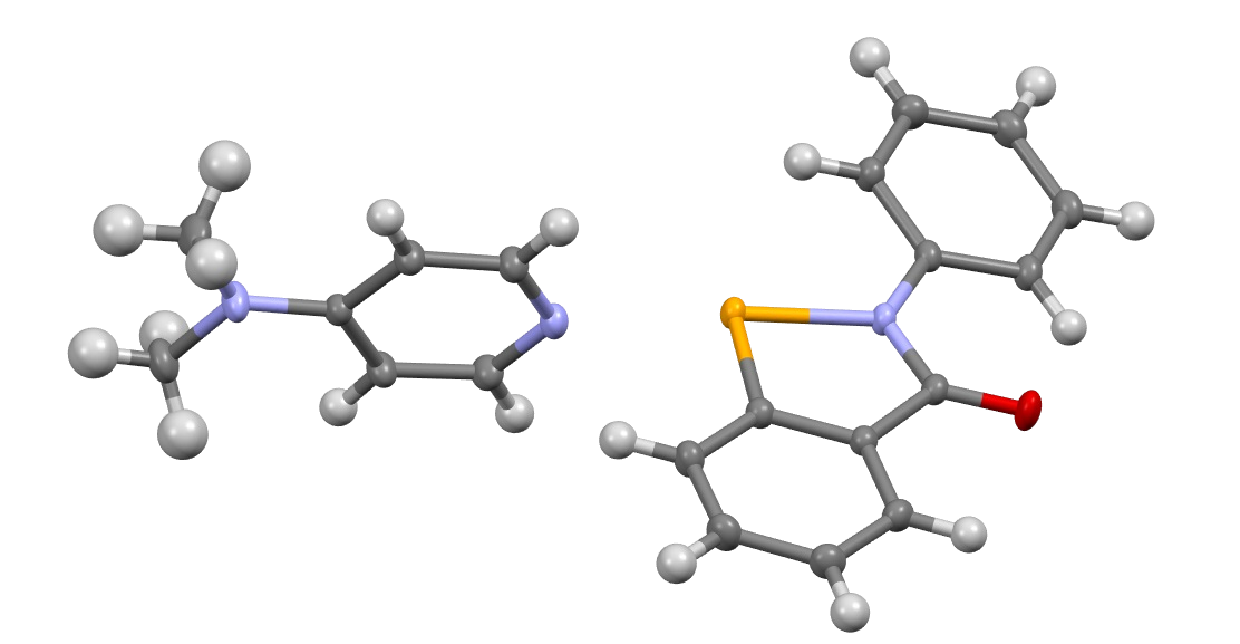
\includegraphics[width=0.6\linewidth]{Figures/ebs-dmap-xtal.pdf}
      \caption{X-ray crystal structure of \texorpdfstring{\refcmpd{ebs}$ \cdot $DMAP}{C20H19N3OSe}.}
    \end{figure}
    
    \subsubsection{Crystal data for \texorpdfstring{\refcmpd{ebs.bn}}{C14H11NOSe}}
    \ce{C14H11NOSe}, $M=288.20$, $T=100.0$~K, $ \lambda=0.71073 $~\AA, Orthorhombic, space group Pca2\textsubscript{1}, $a = 11.7848(3)$, $b = 4.5869(1)$, $c = 21.3572(5)$~\AA, $V = 1154.48(5)$~\AA$^{3}$, $Z = 4$.
    $D_{c}= 1.658$~mg~M$^{-3}$, $\mu$(Mo-K$\alpha$) = 3.233~mm$^{-1}$, F(000) = 576, crystal size $0.63 \times 0.54 \times 0.22$~mm.
    44918 reflections measured, $\theta_{\max}=45.38$\degree, 9588 independent reflections, R\textsubscript{int} = 0.0481, the final R was 0.0331 ($I > 2\theta(I)$, 7848 reflections) and \textit{w}R(F\textsuperscript{2}) was 0.0792 (all data), GOF 1.063.
    CCDC 1867211.
    
    \begin{figure}
      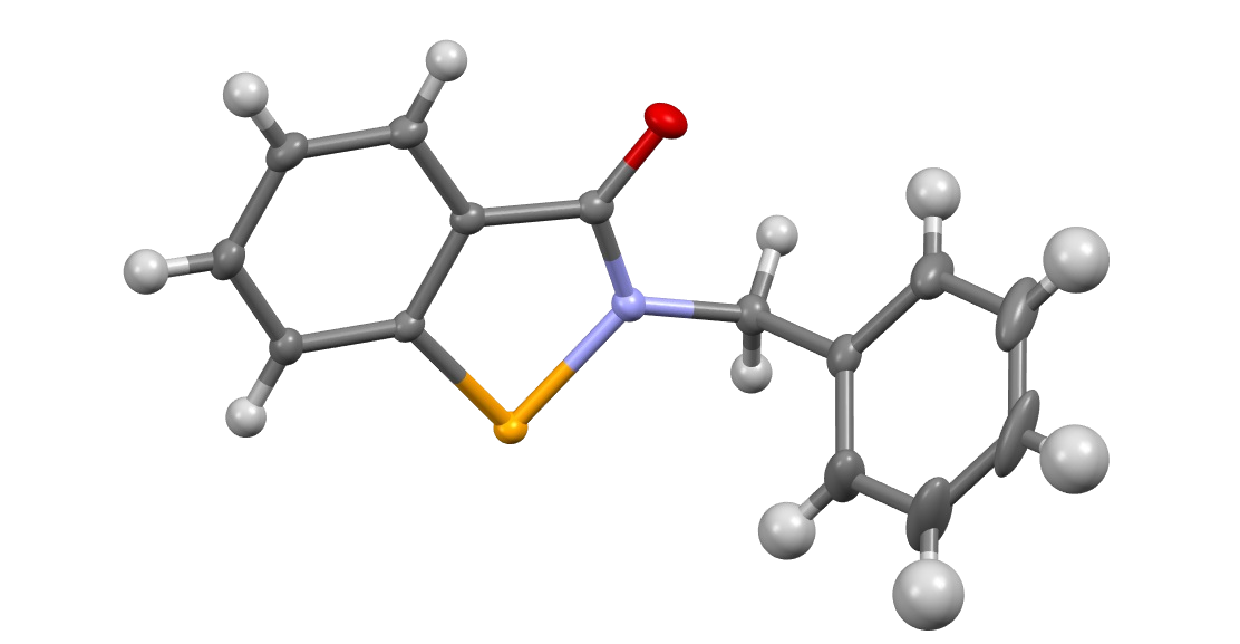
\includegraphics[width=0.6\linewidth]{Figures/ebs-bn-xtal.pdf}
      \caption{X-ray crystal structure of \texorpdfstring{\refcmpd{ebs.bn}}{C14H11NOSe}.}
    \end{figure}
    
    \subsubsection{Crystal data for \texorpdfstring{\refcmpd{ebs.bn}$ \cdot $DMAP$ \cdot $\ce{H2O}}{C21H21N3OSe.(H2O)}}
    \ce{C21H21N3OSe.(H2O)}, $M=428.38$, $T=200.0$~K, $ \lambda=0.71073 $~\AA, Triclinic, space group P$\bar{1}$, $a = 9.6254(2)$, $b = 10.2486(2)$, $c = 10.6505(2)$~\AA, $\alpha = 83.660(2)$\degree, $\beta = 76.398(2)$\degree, $\gamma = 78.423(2)$\degree, $V = 998.19(4)$~\AA$^{3}$, $Z = 2$.
    $D_{c}= 125$~mg~M$^{-3}$, $\mu$(Mo-K$\alpha$) = 1.901~mm$^{-1}$, F(000) = 440, crystal size $0.41 \times 0.32 \times 0.23$~mm.
    30047 reflections measured, $\theta_{\max} = 41.06$\degree, 12528 independent reflections, R\textsubscript{int} = 0.0267, the final R was 0.0456 ($I > 2\theta(I)$, 6303 reflections) and \textit{w}R(F\textsuperscript{2}) was 0.1219 (all data), GOF 1.000.
    CCDC 1867213.
    From THF in an open flask (90\%) m.p. 96--97\degree{}C.
    
    \begin{figure}
      \includegraphics[width=0.6\linewidth]{Figures/ebs-bn-dmap-hydrate-xtal.pdf}
      \caption{X-ray crystal structure of \texorpdfstring{\refcmpd{ebs.bn}$ \cdot $DMAP$ \cdot $\ce{H2O}}{C21H21N3OSe.(H2O)}.}
    \end{figure}
    
    \subsubsection{Crystal data for \texorpdfstring{\refcmpd{ebs.bn}$ \cdot $DMAP}{C21H21N3OSe}}
    \ce{C21H21N3OSe}, $M=410.37$, $T=130.0$~K, $ \lambda=0.71073 $~\AA, Triclinic, space group P$\bar{1}$, $a = 9.6002(4)$, $b = 10.2109(4)$, $c = 19.8380(7)$~\AA, $\alpha = 78.710(3)$\degree, $\beta = 84.901(3)$\degree, $\gamma = 77.458(4)$\degree, $V = 1859.33(13)$~\AA$^{3}$, $Z = 4$, $Z\prime = 2$.
    $D_{c}= 1.466$~mg~M$^{-3}$, $\mu$(Mo-K$\alpha$) = 2.034~mm$^{-1}$, F(000) = 840, crystal size $0.65 \times 0.24 \times 0.37$~mm.
    36541 reflections measured, $\theta_{\max} = 40.95$\degree, 23437 independent reflections, R\textsubscript{int} = 0.0264, the final R was 0.0448 ($I > 2\theta(I)$, 15177 reflections) and \textit{w}R(F\textsuperscript{2}) was 0.1120 (all data), GOF 1.044.
    CCDC 1867209.
    From dichloromethane/pentane (60\%) m.p. 86.1--92.5\degree{}C.
    
    \begin{figure}
      \includegraphics[width=0.6\linewidth]{Figures/ebs-bn-dmap-xtal.pdf}
      \caption{X-ray crystal structure of \texorpdfstring{\refcmpd{ebs.bn}$ \cdot $DMAP}{C21H21N3OSe}.}
    \end{figure}
    
    \subsubsection{Crystal data for \texorpdfstring{\refcmpd{ebs.bn}$ \cdot $quinuclidine}{C21H24N2OSe}}
    \ce{C21H24N2OSe}, $M=399.38$, $T=130.0$~K, $\lambda=1.54184$~\AA, Monoclinic, space group P2\textsubscript{1}/c, $a = 10.1610(2)$, $b = 16.0506(3)$, $c = 11.4300(2)$~\AA, $\beta = 104.622(2)$\degree, $V = 1803.75(6)$ \AA$^{3}$, $Z = 4$.
    $D_{c}= 1.471$~mg~M$^{-3}$, $\mu$(Cu-K$\alpha$) = 3.895~mm$^{-1}$, F(000) = 824, crystal size $0.29 \times 0.10 \times 0.03$~mm.
    12588 reflections measured, $\theta_{\max} = 77.19$\degree, 3771 independent reflections, R\textsubscript{int} = 0.0379, the final R was 0.0329 ($I > 2\theta(I)$, 3397 reflections) and \textit{w}R(F\textsuperscript{2}) was 0.0849 (all data), GOF 1.028.
    CCDC 1867207.
    From dichloromethane/pentane (50\%) m.p. 135.2--137.4\degree{}C.
    
    \begin{figure}
      \includegraphics[width=0.6\linewidth]{Figures/ebs-bn-quin-xtal.pdf}
      \caption{X-ray crystal structure of \texorpdfstring{\refcmpd{ebs.bn}$ \cdot $quinuclidine}{C21H24N2OSe}.}
    \end{figure}
    
    \subsubsection{Crystal data for \texorpdfstring{\refcmpd{ebs.bn}$ \cdot $DABCO}{C20H23N3OSe}}
    \ce{C20H23N3OSe}, $M=400.37$, $T=130.0$~K, $\lambda=1.54184$~\AA, Monoclinic, space group P2\textsubscript{1}/c, $a = 10.1249(2)$, $b = 15.9246(3)$, $c = 11.4660(2)$~\AA, $\beta = 106.572(2)$\degree, $V = 1771.93(6)$ \AA$^{3}$, $Z = 4$.
    $D_{c} = 1.501$~mg~M$^{-3}$, $\mu$(Cu-K$\alpha$) = 2.965~mm$^{-1}$, F(000) = 824, crystal size $0.37 \times 0.17 \times 0.04$~mm.
    13121 reflections measured, $\theta_{\max} = 77.12$\degree, 3711 independent reflections, R\textsubscript{int} = 0.0280, the final R was 0.0258 ($I > 2\theta(I)$, 3333 reflections) and \textit{w}R(F\textsuperscript{2}) was 0.0657 (all data), GOF 1.056.
    CCDC 1867206.
    From dichloromethane/pentane (65\%) m.p. 131.4--133.3\degree{}C.
    
    \begin{figure}
      \includegraphics[width=0.6\linewidth]{Figures/ebs-bn-dabco-xtal.pdf}
      \caption{X-ray crystal structure of \texorpdfstring{\refcmpd{ebs.bn}$ \cdot $DABCO}{C20H23N3OSe}.}
    \end{figure}
    
    \subsubsection{Crystal data for \texorpdfstring{\refcmpd{tetracycle}}{C14H8N2OSe}}
    \ce{C14H8N2OSe}, $M=299.18$, $T=100.0$~K, $\lambda=0.71092$~\AA, Orthorhombic, space group Pca2\textsubscript{1}, $a = 17.371(4)$, $b = 5.3080(11)$, $c = 11.633(2)$~\AA, $V = 1072.6(4)$~\AA$^{3}$, $Z = 4$.
    $D_{c}= 1.853$~mg~M$^{-3}$, $\mu$(Mo-K$\alpha$) = 3.486~mm$^{-1}$, F(000) = 592, crystal size $0.15 \times 0.10 \times 0.02$~mm.
    16031 reflections measured, $\theta_{\max}=31.56$\degree, 2967 independent reflections, R\textsubscript{int} = 0.0363, the final R was 0.0271 ($I > 2\theta(I)$, 2061 reflections) and \textit{w}R(F\textsuperscript{2}) was 0.0751 (all data), GOF 1.129.
    CCDC 1867208.
    
    \begin{figure}
      \includegraphics[width=0.6\linewidth]{Figures/tetracycle-xtal.pdf}
      \caption{X-ray crystal structure of \texorpdfstring{\refcmpd{tetracycle}}{C14H8N2OSe}.}
    \end{figure}
    
    \subsubsection{Crystal data for \texorpdfstring{\refcmpd{tetracycle}$ \cdot $pyridine}{C19H13N3OSe}}
    \ce{C19H13N3OSe}, $M=378.28$, $T=130.0$~K, $\lambda=1.54184$~\AA, Monoclinic, space group P2\textsubscript{1}/c, $a = 20.7476(9)$, $b = 4.9407(2)$, $c = 17.6687(7)$~\AA, $\beta = 107.376(4)$\degree, $V = 1156.27(5)$ \AA$^{3}$, $Z = 4$.
    $D_{c} = 1.454$~mg~M$^{-3}$, $\mu$(Cu-K$\alpha$) = 3.018~mm$^{-1}$, F(000) = 760, crystal size $0.56 \times 0.05 \times 0.03$~mm.
    5766 reflections measured, $\theta_{\max} = 75.76$\degree, 3419 independent reflections, R\textsubscript{int} = 0.0301, the final R was 0.0346 ($I > 2\theta(I)$, 2889 reflections) and \textit{w}R(F\textsuperscript{2}) was 0.0955 (all data), GOF 1.054.
    CCDC 1867211.
    From dichloromethane/pentane (70\%) m.p. 247.5--248.4\degree{}C.
    
    \begin{figure}
      \includegraphics[width=0.6\linewidth]{Figures/tetracycle-py-xtal.pdf}
      \caption{X-ray crystal structure of \texorpdfstring{\refcmpd{tetracycle}$ \cdot $pyridine}{C19H13N3OSe}.}
    \end{figure}
    
    \subsubsection{Crystal data for \texorpdfstring{\refcmpd{tetracycle}$ \cdot $DMAP}{C21H18N4OSe}}
    \ce{C21H18N4OSe}, $M = 421.35$, $T=100.0$~K, $ \lambda=0.71073 $~\AA, Triclinic, space group P$\bar{1}$, $a = 8.8093(2)$, $b = 10.7445(2)$, $c = 10.9812(2)$~\AA, $\alpha = 111.687(2)$\degree, $\beta = 109.283(2)$\degree, $\gamma = 96.631(2)$\degree, $V = 877.57(3)$~\AA$^{3}$, $Z = 2$, $Z\prime = 2$.
    $D_{c}= 1.595$~mg~M$^{-3}$, $\mu$(Mo-K$\alpha$) = 2.159~mm$^{-1}$, F(000) = 428, crystal size $0.18 \times 0.11 \times 0.06$~mm.
    56053 reflections measured, $\theta_{\max} = 41.07$\degree, 11273 independent reflections, R\textsubscript{int} = 0.0547, the final R was 0.0358 ($I > 2\theta(I)$, 8667 reflections) and \textit{w}R(F\textsuperscript{2}) was 0.0872 (all data), GOF 1.048.
    CCDC 1867212.
    From dichloromethane/pentane (80\%) m.p. 248.8--249.4\degree{}C.
    
    \begin{figure}
      \includegraphics[width=0.6\linewidth]{Figures/tetracycle-dmap-xtal.pdf}
      \caption{X-ray crystal structure of \texorpdfstring{\refcmpd{tetracycle}$ \cdot $DMAP}{C21H18N4OSe}.}
    \end{figure}
    
    \printbibliography[heading=subbibliography]
    \end{refsection}
    

\begin{refsection}

\chapter{Further investigations into Ch-bonded complexes}\label{ch:hammett}

\section{Introduction}
In the previous chapter, we established that Ch-bonding is not only present in ebselen derivatives, but dominates packing in crystals of the pure compound (through \ce{Se\cdots O} interactions) and in co-crystals with a variety of Lewis bases.
In this chapter, we extend our investigation to a wider range of derivatives with systematically varied electronic properties.

Linear free energy relationships (LFERs) relate the rate of a chemical reaction with some electronic property of the substrate molecule(s).
Although the single crystal structures presented here are \emph{static} snapshots of reality, we can think of them as representative of progress toward the transition state for a particular reaction, in this case the formation of a \ce{N_{base} \cdots Se} bond and the concomitant breaking of the endocyclic \ce{Se-N} bond (\cref{fig:bond-breaking}).
The lower the transition state energy, the shorter will be the \ce{Se\cdots N} Ch-bond distance, and this is clearly influenced by the electronic properties of both the Ch-bond donor and acceptor.
They have been used previously to explain trends in X-bonding.\autocite{Laurence1983,Sarwar2010}

\begin{figure}
  \includegraphics[scale=0.74]{Figures/bond-breaking.eps}
  \caption[Nucleophilic substitution at selenium.]{Depiction of the bond breaking/forming process of which Ch-bonding is a ground state manifestation.}\label{fig:bond-breaking}
\end{figure}

\section{Results and discussion}

\begin{comment}
\begin{scheme}
  \centering
  \replacecmpd[sub-only]{py.pyrrol}
  \replacecmpd[sub-only]{py.morph}
  \replacecmpd{py.pyrrol,py.morph}
  \includegraphics[scale=0.74]{Figures/base-synthesis.eps}
  \caption{Synthesis of Lewis bases \refcmpd{py.pyrrol,py.morph}.}\label{sch:base-synthesis}
\end{scheme}
\end{comment}
  
Our previous work had shown that electron-rich pyridines (specifically DMAP) formed the strongest Ch-bonds out of all the bases trialled (\cref{ch:crystengcomm1}).
This is roughly consistent with the hydrogen bond basicity (pK\textsubscript{HB}) of the bases (\cref{tab:pkhb}).
The planar geometry and aromatic character of DMAP may also facilitate crystallisation, as opposed to the relatively bulky and flexible aliphatic bases which may not pack as efficiently.
For these reasons, we restricted the bases used in this study to other electron-rich pyridines.

\begin{figure}
  \centering
  \replacecmpd{py.morph}
  \replacecmpd{py.pyrrol}
  \includegraphics[scale=0.74]{Figures/bases.eps}
  \caption[Lewis bases used in this work.]{Lewis bases used in this work in order of increasing basicity.}\label{fig:bases}
\end{figure}

Although DMAP is already a very strong base, the basicity can be increased by incorporating the aniline nitrogen in another ring.
This reduces the energetic penalty associated with the delocalisation of the lone pair into the pyridine ring, by forcing a more planar geometry upon the nitrogen.\autocite{Berthelot1998,Heinrich2003EnhancingFixation}
%Compounds \cmpd{py.pyrrol,py.morph} were therefore synthesised by treating 4-chloropyridine hydrochloride with 2 equivalents of the appropriate base (\cref{sch:base-synthesis}).
We therefore prepared co-crystals with \cmpd{py.morph,py.pyrrol}, which are slightly weaker and stronger bases than DMAP respectively (\cref{fig:bases}).
\cmpd{py.pyrrol} is a stronger base due to the imposed planarity of the aniline nitrogen, while \cmpd{py.morph} is weaker due to the larger ring and electron withdrawing oxygen atom.

\begin{scheme}
  \centering
  \replacecmpd{diselenide}
  \replacecmpd[merge=false,compress=false]{ebs}
  \includegraphics[scale=0.74]{Figures/ebs-synthesis.eps}
  
  \begin{comment}
  \vspace{0.6cm}
  
  \footnotesize{
  \begin{tabular}{cccccc}\toprule
      Compound & R = & Compound & R = & Compound & R = \\\midrule
      \cmpd{ebs} & \ce{-H} & \cmpd{ebs.4cf3} & \ce{-CF3} & \cmpd{ebs.4me} & \ce{-CH3}\\
      \cmpd{ebs.4no2} & \ce{-NO2} & \cmpd{ebs.4br} & \ce{-Br} & \cmpd{ebs.4ome} & \ce{-OMe}\\
      \cmpd{ebs.4cn} & \ce{-CN} & \cmpd{ebs.4co2et} & \ce{-CO2Et} & \cmpd{ebs.4oet} & \ce{-OEt} \\\bottomrule
  \end{tabular}}
  \end{comment}
  
  \caption[Synthesis of benzisoselenazolinone derivatives.]{Synthesis of benzisoselenazolinone derivatives.\@ (a) 1. \ce{NaNO2}, \ce{HCl}, 0\degree{}C;\@ 2. \ce{Na2Se2}, \ce{NaOH}, rt, 1~h, 37\%; (b) 1. \ce{SOCl2}, cat. DMF, reflux, 1.5~h; 2. \ce{ArNH2}, TEA, MeCN, rt, 2~h, 14--67\%.}\label{sch:ebs-synthesis}
  \end{scheme}

The benzisoselenazolinone derivatives \cmpd[merge=false,compress=false]{ebs,ebs.{4no2,4cn,4cf3,4br,4co2et,4me,4ome,4oet}} were prepared by the reaction of substituted anilines with the dichloride of \cmpd{diselenide}, which was ultimately derived from anthranilic acid (\cref{sch:ebs-synthesis}).
The one-pot selenocyclisation reaction used in \cref{ch:crystengcomm1} often did not tolerate the various functional groups on the aryl ring, affording reduction, cross-coupling, or protodehalogenation byproducts.
All derivatives except \cmpd{ebs.4no2} were isolated in acceptable yield at room temperature using acetonitrile as a solvent, and in the presence of a weak base (triethylamine).
Due to the strongly electron-withdrawing nature of the nitro substituent, the parent aniline of \cmpd{ebs.4no2} was not sufficiently nucleophilic to react under the same conditions.
We therefore first deprotonated the aniline using \ce{NaH} (60\% suspension in mineral oil) in anhydrous THF before adding the selenenyl chloride, which afforded the benzisoselenazolinone in excellent yield.

Co-crystals of the benzisoselenazolinones and pyridines were grown by vapour diffusion from an equimolar solution in dichloromethane/pentane.
Relevant structural parameters are given in \cref{tab:bondlengths2}.
In addition to the structural parameters, we characterised the various Ch-bonds using Bader's QTAIM framework.
Depending on the quality of the data we were able to obtain for each crystal, we used:

\begin{itemize}
    \item experimental electron density from a multipole refinement with atomic coordinates determined from high angle refinement ($d < 0.8$\AA),
    \item experimental electron density from a multipole refinement with atomic coordinates determined by refinement using aspherical scattering factors derived from the DFT electron density,
    \item density derived from a DFT calculation on the crystal geometry.
\end{itemize}

The second ``hybrid'' strategy has the advantage of being able to capture electron density effects not fully described by DFT, while not requiring a large amount of weak high-angle (or neutron) data for the reliable determination of atomic coordinates.
The low-angle data, however, does need to be free from faults, so this strategy may still not be appropriate for all data sets.
For the second and third strategies, the densities and scattering factors were calculated using NoSpherA2 incorporated in Olex2.3.\autocite{Kleemiss2021}

\begin{figure}
  \includegraphics[width=0.6\linewidth]{Figures/rho-agreement.eps}
  \caption[Experimental vs calculated electron density.]{Experimental vs calculated electron density. The dotted line represents $\rho_\text{BCP, exp} = \rho_\text{BCP, calc}$. $R^2 = 0.8660$.}\label{fig:qtaim-calc-exp}
\end{figure}

In order to ensure that we were not introducing errors in the electron density parameters by using data from several sources (experimental vs calculated), we calculated the electron density for \emph{all} complexes and compared the QTAIM parameters to the experimental ones where possible.
Fortunately, adequate agreement was obtained ($R^2 = 0.8660$, \cref{fig:qtaim-calc-exp}).
There does appear to be a slight bias towards scatter above the line, indicating that the calculation underestimates the electron density.
Although the $\omega$B97X-D functional is very good at describing non-bonded complexes in terms of energy, electron density is not a typical benchmarking criterion, so it is perhaps not surprising that it is not in full agreement with experimental measurements.


\begin{figure}
  \includegraphics[width=0.7\linewidth]{Figures/ebs-dmap-bondlengths.pdf}
  \caption{Geometric parameters indicated in \cref{tab:bondlengths2}.}\label{fig:ebs-dmap-bondlengths}
\end{figure}

\begin{table}
  \centering
  \caption[Selected structural and electron density parameters of Ch-bonded complexes.]{Selected structural and electron density parameters of Ch-bonded complexes. See \cref{fig:ebs-dmap-bondlengths} for depiction of parameters.}\label{tab:bondlengths2}

  \small
  \tablefit{\begin{tabular}{lllllllll}
    \toprule
    Complex & r(\ce{N \cdots Se}) & r(\ce{Se-N_{1}}) & r(Se--C\textsubscript{1}) & r(N\textsubscript{1}--C(O)) & $ \angle $(N$ \cdots $\ce{Se-N_{1}}) & $ \angle $(C\textsubscript{para}$ \cdots $\ce{N \cdots Se}) & $\rho_{\text{BCP}}$(\ce{Se\cdots N}) & $\nabla^{2}(\rho_{\text{BCP}})$(\ce{Se\cdots N}) \\
      & \AA\ & \AA\ & \AA\ & \AA\ & \degree\ & \degree\ & e/\AA$^3$ & e/\AA$^5$ \\ \midrule
    \cmpd{ebs}                       & --- & 1.896(3) & 1.892(4) & 1.359(5) & --- & --- & --- & --- \\
    \cmpd{ebs.4no2}                     & --- \\
    \cmpd{ebs.4cn}                      & --- & 1.894(2) & 1.877(2) & 1.372(2) & --- & --- & --- & --- \\
    \cmpd{ebs.4cf3}\footnote{\label{fn:enva}Environment \textit{a}} & --- & 1.880(9) & 1.889(9) & 1.38(1) & --- & --- & --- & --- \\
    \cmpd{ebs.4cf3}\footnote{\label{fn:envb}Environment \textit{b}} & --- & 1.898(8) & 1.901(9) & 1.37(1) & --- & --- & --- & --- \\
    \cmpd{ebs.4br}                      & --- & 1.898(2) & 1.889(2) & 1.371(3) & --- & --- & --- & --- \\
    \cmpd{ebs.4co2et}                   & --- & 1.902(2) & 1.879(2) & 1.371(3) & --- & --- & --- & --- \\
    \cmpd{ebs.4me}                      & --- & 1.904(3) & 1.890(3) & 1.365(4) & --- & --- & --- & --- \\
    \cmpd{ebs.4ome}                     & --- & 1.8741(9) & 1.887(1) & 1.356(1) & --- & --- & --- & --- \\
    \cmpd{ebs.4oet}                     & --- & 1.901(3) & 1.885(4) & 1.357(4) & --- & --- & --- & --- \\ \\ 

    \cmpd{ebs}$ \cdot $DMAP     & 2.371(1) & 1.968(1) & 1.896(1) & 1.358(2) & 174.18(4) & 173.51(6) & 0.3511 & 2.6960\footnote{\label{fn:fullmultipole}Fully experimental density used} \\
    \cmpd{ebs.4no2}$ \cdot $DMAP   & 2.2424(5) & 2.0200(4) & 1.9086(4) & 1.3592(4) & 173.57(2) & 175.47(2) & 0.4772 & 3.8680\textsuperscript{\ref{fn:fullmultipole}} \\
    \cmpd{ebs.4cn}$ \cdot $DMAP    & 2.301(1) & 1.997(1) & 1.899(2) & 1.368(2) & 174.79(5) & 167.57(6) & 0.4130 & 2.5210\textsuperscript{\ref{fn:fullmultipole}} \\
    \cmpd{ebs.4cn}$ \cdot $DMAP\footnote{\label{fn:solvate}DCM solvate}\textsuperscript{,\ref{fn:enva}}  & 2.254(2) & 2.019(2) & 1.902(1) & 1.366(2) & 174.46(6) & 176.33(7) & 0.4780 & 2.4816\footnote{\label{fn:dftdens}DFT density used} \\
    \cmpd{ebs.4cn}$ \cdot $DMAP\textsuperscript{\ref{fn:solvate},\ref{fn:envb}}  & 2.308(2) & 1.993(1) & 1.901(1) & 1.372(2) & 174.93(5) & 167.85(7) & 0.4284 & 2.4558 \textsuperscript{\ref{fn:dftdens}} \\
    \cmpd{ebs.4cf3}$ \cdot $DMAP   & 2.3347(9) & 1.9855(9) & 1.899(1) & 1.372(1) & 175.24(4) & 162.65(5) & 0.4048 & 2.4112\textsuperscript{\ref{fn:dftdens}}\\
    \cmpd{ebs.4br}$ \cdot $DMAP    & 2.3215(7) & 1.9840(7) & 1.9021(8) & 1.362(1) & 173.85(3) & 173.56(4) & 0.4058 & 3.1160\textsuperscript{\ref{fn:fullmultipole}}\\
    \cmpd{ebs.4co2et}$ \cdot $DMAP\textsuperscript{\ref{fn:solvate}} & 2.322(1) & 1.982(1) & 1.902(1) & 1.367(2) & 174.96(4) & 172.86(6) & 0.4143 & 2.4585\textsuperscript{\ref{fn:dftdens}} \\
    \cmpd{ebs.4me}$ \cdot $DMAP    & 2.4301(4) & 1.9341(4) & 1.8918(4) & 1.3650(6) & 175.33(1) & 158.64(2) & 0.2843 & 3.2570\textsuperscript{\ref{fn:fullmultipole}}\\
    \cmpd{ebs.4ome}$ \cdot $DMAP\footnote{\label{fn:p1}Polymorph 1}\textsuperscript{,\ref{fn:enva}} & 2.270(1) & 1.9689(9) & 1.899(1) & 1.350(1) & 174.17(3) & 159.44(4) & 0.4545 & 2.5544\textsuperscript{\ref{fn:dftdens}}\\
    \cmpd{ebs.4ome}$ \cdot $DMAP\textsuperscript{\ref{fn:p1},\ref{fn:envb}}  & 2.4496(9) & 1.9267(9) & 1.895(1) & 1.357(1) & 174.57(3) & 160.53(4) & 0.3207 & 2.1731\textsuperscript{\ref{fn:dftdens}}\\
    \cmpd{ebs.4ome}$ \cdot $DMAP\footnote{\label{fn:p2}Polymorph 2}\textsuperscript{,\ref{fn:enva}}  & 2.334(1) & 1.965(1) & 1.894(1) & 1.363(1) & 175.95(5) & 155.71(6) & 0.4421 & 3.1590\textsuperscript{\ref{fn:fullmultipole}}\\
    \cmpd{ebs.4ome}$ \cdot $DMAP\textsuperscript{\ref{fn:p2},\ref{fn:envb}}  & 2.407(1) & 1.941(1) & 1.894(1) & 1.358(2) & 176.12(5) & 156.60(6) & 0.3806 & 2.9170\textsuperscript{\ref{fn:fullmultipole}}\\
    \cmpd{ebs.4oet}$ \cdot $DMAP\textsuperscript{\ref{fn:enva}}   & 2.517(2) & 1.921(1) & 1.895(2) & 1.356(3) & 172.30(6) & 158.37(8) & 0.3641 & 2.9344\textsuperscript{\ref{fn:fullmultipole}}\\
    \cmpd{ebs.4oet}$ \cdot $DMAP\textsuperscript{\ref{fn:envb}}   & 2.327(5) & 1.931(2) & 1.894(2) & 1.353(3) & 171.4(1) & 151.2(3) & 0.2565 & 2.3493\textsuperscript{\ref{fn:fullmultipole}}\\ \\

    \cmpd{ebs}$ \cdot $\cmpd{py.morph}\textsuperscript{\ref{fn:p1}}      & 2.414(2) & 1.960(2) & 1.902(2) & 1.366(2) & 175.46(6) & 166.23(8) & 0.3396 & 2.3328\textsuperscript{\ref{fn:dftdens}}\\
    \cmpd{ebs}$ \cdot $\cmpd{py.morph}\textsuperscript{\ref{fn:p2}}      & 2.420(2) & 1.967(2) & 1.903(2) & 1.363(2) & 176.7(1) & 174.23(8) & 0.3416 & 2.2739\textsuperscript{\ref{fn:dftdens}}\\
    \cmpd{ebs.4no2}$ \cdot $\cmpd{py.morph}   & --- \\
    \cmpd{ebs.4cn}$ \cdot $\cmpd{py.morph}\textsuperscript{\ref{fn:solvate}}    & 2.301(1) & 1.993(1) & 1.907(1) & 1.368(2) & 173.08(5) & 164.75(6) & 0.4306 & 2.4546\footnote{\label{fn:hybrid}Hybrid density used} \\
    \cmpd{ebs.4cf3}$ \cdot $\cmpd{py.morph}   & --- \\
    \cmpd{ebs.4br}$ \cdot $\cmpd{py.morph}    & 2.381(2) & 1.975(2) & 1.905(2) & 1.367(2) & 173.84(6) & 174.97(8) & 0.3620 & 2.3519\textsuperscript{\ref{fn:dftdens}}\\
    \cmpd{ebs.4co2et}$ \cdot $\cmpd{py.morph} & 2.337(3) & 1.982(3) & 1.906(4) & 1.374(5) & 173.5(1) & 170.1(2) & 0.4286 & 2.4674\textsuperscript{\ref{fn:dftdens}}\\
    \cmpd{ebs.4me}$ \cdot $\cmpd{py.morph}    & 2.412(5) & 1.977(5) & 1.908(5) & 1.360(7) & 174.4(2) & 178.9(2) & 0.3456 & 2.2774\textsuperscript{\ref{fn:dftdens}}\\
    \cmpd{ebs.4ome}$ \cdot $\cmpd{py.morph}   & --- \\
    \cmpd{ebs.4oet}$ \cdot $\cmpd{py.morph}\textsuperscript{\ref{fn:enva}}    & 2.398(4) & 1.958(4) & 1.894(6) & 1.367(6) & 174.6(2) & 174.1(2) & 0.3553 & 2.3309\textsuperscript{\ref{fn:dftdens}}\\
    \cmpd{ebs.4oet}$ \cdot $\cmpd{py.morph}\textsuperscript{\ref{fn:envb}}    & 2.448(6) & 1.951(4) & 1.901(5) & 1.367(5) & 175.5(2) & 170.5(3) & 0.3239 & 2.2095\textsuperscript{\ref{fn:dftdens}}\\ \\

    \cmpd{ebs}$ \cdot $\cmpd{py.pyrrol}     & 2.350(1) & 1.9830(9) & 1.8985(7) & 1.3616(8) & 174.20(3) & 176.46(4) & 0.3867 & 2.4117\textsuperscript{\ref{fn:dftdens}}\\
    \cmpd{ebs.4no2}$ \cdot $\cmpd{py.pyrrol}   & --- \\
    \cmpd{ebs.4cn}$ \cdot $\cmpd{py.pyrrol}    & 2.289(1) & 2.000(1) & 1.902(1) & 1.363(2) & 174.77(5) & 175.06(7) & 0.4403 & 2.4424\textsuperscript{\ref{fn:dftdens}} \\
    \cmpd{ebs.4cf3}$ \cdot $\cmpd{py.pyrrol}   & --- \\
    \cmpd{ebs.4br}$ \cdot $\cmpd{py.pyrrol}    & 2.319(2) & 1.981(2) & 1.895(1) & 1.362(2) & 174.57(6) & 174.60(8) & 0.4106 & 2.4504\textsuperscript{\ref{fn:dftdens}}\\
    \cmpd{ebs.4co2et}$ \cdot $\cmpd{py.pyrrol} & 2.337(3) & 1.982(3) & 1.906(4) & 1.374(5) & 173.5(1) & 170.1(2) & 0.4014 & 2.4107\textsuperscript{\ref{fn:dftdens}}\\
    \cmpd{ebs.4me}$ \cdot $\cmpd{py.pyrrol}    & 2.272(1) & 1.986(1) & 1.905(1) & 1.351(2) & 172.66(5) & 173.51(6) & 0.4545 & 2.5279\textsuperscript{\ref{fn:dftdens}}\\
    \cmpd{ebs.4ome}$ \cdot $\cmpd{py.pyrrol}   & --- \\
    \cmpd{ebs.4oet}$ \cdot $\cmpd{py.pyrrol}\textsuperscript{\ref{fn:enva}}   & 2.356(3) & 1.972(3) & 1.898(3) & 1.355(4) & 174.5(1) & 170.2(1) & 0.3878 & 2.4124\textsuperscript{\ref{fn:dftdens}}\\
    \cmpd{ebs.4oet}$ \cdot $\cmpd{py.pyrrol}\textsuperscript{\ref{fn:envb}}   & 2.371(3) & 1.964(3) & 1.898(3) & 1.360(4) & 174.9(1) & 170.9(1) & 0.3774 & 2.3640\textsuperscript{\ref{fn:dftdens}}\\
    \bottomrule
    \end{tabular}}
\end{table}

\subsection{Hammett plots of crystallographic data}
Evident in this data is a trend of increasing Ch-bond length with increasing electron donating character of the substituent.
There are a number of methods to quantify this property of the substituent, the most well-known being the Hammett substituent parameters.
The Hammett \textit{para} substituent parameter $ \sigma_\text{p} $ for a given substituent at the \textit{para} position is determined from the ionisation equilibrium of the parent carboxylic acid.
Although originally used to explain reaction kinetics with an associated reaction constant $\rho$, the substituent constant provides a convenient measure of electronic character for ground state phenomena as well.
Within the context of Ch-bonding, this can be rationalised by considering the approach of the Lewis base to form the Ch-bond as an incipient nucleophilic substitution at the selenium, and invoking the Hammond postulate to relate the transition state geometry to the ground state (\cref{fig:bond-breaking}).

Closely linked to the substituent constant $ \sigma_\text{p} $ are the values of $\sigma_\text{p}^{+}$ and $\sigma_\text{p}^{-}$, which can be used when mesomeric effects have a strong influence on the property being studied.
The substituent constant $ \sigma_\text{m} $ is used when the functional group is \textit{meta} to the position of interest.
Hammett substituent parameters are particularly convenient as they have been determined for a wide variety of substituents.
Parameters for the following analysis were obtained from reference~\cite{Hansch1991}.

\begin{figure}
    \centering
    \includegraphics[width=0.9\linewidth]{Figures/hammett-endo-free.eps}
    \caption{Hammett plot of endocyclic \ce{Se-N} bond length of uncomplexed ebselen derivatives.}\label{fig:hammett-endo-free}
\end{figure}

The structural effects most relevant to Ch-bonding will manifest themselves in the vicinity of the selenium atom.
Of particular interest is the endocyclic \ce{Se-N} bond length, which serves as a measure of $\sigma^\star$(\ce{Se-N}) orbital occupancy, thus the degree of hyperconjugation and character of the Ch-bond.

\begin{figure}
  \centering
  \includegraphics[width=0.6\linewidth]{Figures/ebs.me-packing.pdf}
  \caption[One dimensional chains formed by Ch-bonding between the selenium and carbonyl oxygen in \refcmpd{ebs.4me}.]{One dimensional chains formed by Ch-bonding between the selenium and carbonyl oxygen in \refcmpd{ebs.4me}. All other ebselen derivatives display a similar packing motif.}\label{fig:ebs-me-packing}
\end{figure}

As can be seen in \cref{fig:hammett-endo-free}, there is practically no correlation between the electronic properties of the aryl ring and the endocyclic \ce{Se-N} bond length in crystals of the unbound ebselen derivatives.
This is not unexpected, as in all cases the crystals consist of one dimensional chains of ebselen molecules Ch-bonded to the carbonyl oxygen of the next (\cref{fig:ebs-me-packing}).
As the magnitude of the $ \sigma $-hole (Ch-bond donor ability) is \emph{increased} by an electron withdrawing substituent, the Ch-bond acceptor ability of the carbonyl is \emph{decreased}.
These opposing effects appear to be approximately equal in magnitude, so cancel each other out and give a very flat and featureless Hammett plot.

\begin{figure}
\centering
\begin{subfigure}[t]{0.45\linewidth}
  \centering
  \includegraphics[width=\linewidth]{Figures/hammett-dmap-p.eps}
  \caption{Ebselen derivatives complexed with DMAP.\@ The lines are described by the equations $\mathrm{r}(\ce{Se-N}) = (1.959(5) + 0.067(10) \times \sigma_\text{p})$~\AA~($R^2=0.7857$) and $\mathrm{r}(\ce{Se\cdots N}) = (2.363(17) - 0.12(4) \times \sigma_\text{p})$~\AA~($R^2=0.4104$).}\label{fig:hammett-dmap-para}
\end{subfigure}
\hfill
\begin{subfigure}[t]{0.45\linewidth}
\centering
\includegraphics[width=\linewidth]{Figures/hammett-morph-p.eps}
\caption{Ebselen derivatives complexed with \refcmpd{py.morph}. The line is described by the equation $\mathrm{r}(\ce{Se-N}) = (1.967(3) + 0.036(9) \times \sigma_\text{p})$~\AA~($R^2=0.7386$) and $\mathrm{r}(\ce{Se\cdots N}) = (2.400(7) - 0.13(2) \times \sigma_\text{p})$~\AA~($R^2=0.8522$).}\label{fig:hammett-morph-para}
\end{subfigure}
\hfill
\begin{subfigure}[t]{0.45\linewidth}
\centering
\includegraphics[width=\linewidth]{Figures/hammett-pyrrol-p.eps}
\caption{Ebselen derivatives complexed with \refcmpd{py.pyrrol}. The lines are described by the equations $\mathrm{r}(\ce{Se-N}) = (1.9761(28) + 0.029(8) \times \sigma_\text{p})$~\AA~($R^2=0.7828$) and $\mathrm{r}(\ce{Se\cdots N}) = (2.347(7) - 0.071(17) \times \sigma_\text{p})$~\AA~($R^2=0.8005$)}\label{fig:hammett-pyrrol-para}
\end{subfigure}
\caption[Hammett plots of endocyclic \ce{Se-N} bond length and \ce{Se\cdots N} Ch-bond length of ebselen derivatives complexed with various Lewis bases ($\sigma_\text{p}$).]{Hammett plots of endocyclic \ce{Se-N} bond length and \ce{Se\cdots N} Ch-bond length of ebselen derivatives complexed with various Lewis bases ($\sigma_\text{p}$). In all Hammett plots, the upper line represents the \ce{Se\cdots N} Ch-bond distance, and the lower line represents the endocyclic \ce{Se-N} bond length.}
\end{figure}

\begin{table}
  \caption{Linear regression results for Hammett plots in \cref{fig:hammett-dmap-para,fig:hammett-pyrrol-para,fig:hammett-morph-para}.}
  \begin{tabular}{llllllll}\toprule
         & \multicolumn{3}{c}{$\mathrm{r}(\ce{Se\cdots N})$} & \multicolumn{3}{c}{$\mathrm{r}(\ce{Se-N})$} \\
         \cmidrule(lr){3-5}\cmidrule(lr){6-8}
    Base            & pK\textsubscript{HB}\autocite{Berthelot1998} & gradient  & intercept & $R^2$ & gradient & intercept & $R^2$ \\\midrule
    \cmpd{py.morph} & 2.68                 & $-0.13(2)$  & 2.400(7)  & 0.8522& 0.036(9) & 1.967(3)& 0.7286 \\
    DMAP            & 2.80                 & $-0.12(4)$  & 2.363(17) & 0.4104& 0.067(10)& 1.959(5)  & 0.7857 \\
    \cmpd{py.pyrrol}& 2.93                 & $-0.071(17)$& 2.347(7)  & 0.8005& 0.029(8) & 1.9761(28)& 0.7828 \\
    \bottomrule 
  \end{tabular}\label{tab:hammett-results-para}
\end{table}

Fortunately, inspecting the same bond length in co-crystals of ebselen derivatives and a Lewis base gives us a much clearer dependence, as can be seen in \cref{fig:hammett-dmap-para,fig:hammett-pyrrol-para,fig:hammett-morph-para}.
This is because the Ch-bond acceptor ability is now independent of the electronic properties of the Ch-bond donor, so the \ce{Se-N} bond length is determined solely by the latter.
An inverse correlation can be seen in the \ce{Se\cdots N} Ch-bond length.
The results are tabulated in \cref{tab:hammett-results-para}.
Moderately good correlation is obtained, as measured by the $R^2$ values, although there is clearly some deviation on the left hand side of the plots where the strongly electron donating substituents are found.
While the more strongly Ch-bonded systems (with electron withdrawing substituents) are generally very well described by the model, the electron rich derivatives \cmpd{ebs.4ome,ebs.4oet} vary significantly in their bond lengths.
Indeed, in the case of DMAP complexes, omitting these data points improves the correlation coefficient to 0.8148 while the gradient and intercept are almost unchanged at $-0.156(28)$~\AA~and $2.386(15)$~\AA~respectively, suggesting that the model is appropriate, and that there is some other effect occurring in electron rich systems.
For a further discussion of this phenomenon, see \cref{sec:z2}.

It has been found that phenomena that are dominated by inductive or field effects are better described by the \textit{meta} substituent constant $\sigma_\text{m}$.\autocite{Reynolds1980,Sarwar2010}
We therefore constructed Hammett plots using this parameter as well, which are shown in \cref{fig:hammett-dmap-meta,fig:hammett-pyrrol-meta,fig:hammett-morph-meta}, and the results tabulated in \cref{tab:hammett-results-meta}.

\begin{figure}
  \centering
\begin{subfigure}[t]{0.45\linewidth}
  \centering
  \includegraphics[width=\linewidth]{Figures/hammett-dmap-m.eps}
  \caption{Ebselen derivatives complexed with DMAP.\@ The lines are described by the equations $\mathrm{r}(\ce{Se-N}) = (1.937(7) + 0.011(2) \times \sigma_\text{m})$~\AA~($R^2=0.7501$) and $\mathrm{r}(\ce{Se\cdots N}) = (2.41(2) - 0.22(6) \times \sigma_\text{m})$~\AA~($R^2=0.4680$).}\label{fig:hammett-dmap-meta}
\end{subfigure}
\hfill
\begin{subfigure}[t]{0.45\linewidth}
\centering
\includegraphics[width=\linewidth]{Figures/hammett-morph-m.eps}
\caption{Ebselen derivatives complexed with \refcmpd{py.morph}. The line is described by the equation $\mathrm{r}(\ce{Se-N}) = (1.963(5) + 0.04(2) \times \sigma_\text{m})$~\AA~($R^2=0.4620$) and $\mathrm{r}(\ce{Se\cdots N}) = (2.42(1) - 0.18(4) \times \sigma_\text{m})$~\AA~($R^2=0.7438$).}\label{fig:hammett-morph-meta}
\end{subfigure}
\hfill
\begin{subfigure}[t]{0.45\linewidth}
  \centering
\includegraphics[width=\linewidth]{Figures/hammett-pyrrol-m.eps}
\caption{Ebselen derivatives complexed with \refcmpd{py.pyrrol}. The lines are described by the equations $\mathrm{r}(\ce{Se-N}) = (1.970(6) + 0.04(2) \times \sigma_\text{m})$~\AA~($R^2=0.5098$) and $\mathrm{r}(\ce{Se\cdots N}) = (2.368(10) - 0.12(3) \times \sigma_\text{m})$~\AA~($R^2=0.7892$)}\label{fig:hammett-pyrrol-meta}
\end{subfigure}
\caption[Hammett plots of endocyclic \ce{Se-N} bond length and \ce{Se\cdots N} Ch-bond length of ebselen derivatives complexed with various Lewis bases ($\sigma_\text{m}$).]{Hammett plots of endocyclic \ce{Se-N} bond length and \ce{Se\cdots N} Ch-bond length of ebselen derivatives complexed with various Lewis bases ($\sigma_\text{m}$). In all Hammett plots, the upper line represents the \ce{Se\cdots N} Ch-bond distance, and the lower line represents the endocyclic \ce{Se-N} bond length.}
\end{figure}

\begin{table}
  \caption{Linear regression results for Hammett plots in \cref{fig:hammett-dmap-meta,fig:hammett-pyrrol-meta,fig:hammett-morph-meta}.}
  \begin{tabular}{llllllll}\toprule
         & \multicolumn{3}{c}{$\mathrm{r}(\ce{Se\cdots N})$} & \multicolumn{3}{c}{$\mathrm{r}(\ce{Se-N})$} \\
         \cmidrule(lr){3-5}\cmidrule(lr){6-8}
    Base            & pK\textsubscript{HB}\autocite{Berthelot1998} & gradient  & intercept & $R^2$ & gradient & intercept & $R^2$ \\\midrule
    \cmpd{py.morph} & 2.68                 & $-0.18(4)$ & 2.42(1)  & 0.7438 & 0.04(2) & 1.963(5) & 0.4620 \\
    DMAP            & 2.80                 & $-0.22(6)$ & 2.41(2)  & 0.4680 & 0.11(2) & 1.937(7) & 0.7501 \\
    \cmpd{py.pyrrol}& 2.93                 & $-0.12(3)$ & 2.368(10)& 0.7892 & 0.04(2) & 1.970(6) & 0.5098 \\
    \bottomrule 
  \end{tabular}\label{tab:hammett-results-meta}
\end{table}

We obtain a slightly poorer fit when using $\sigma_\text{m}$ compared to $\sigma_\text{p}$.
We note, however, that the correlation is well below what would be accepted as ``good'' for a Hammett plot ($R^2 < 0.95$)\autocite{Jaffe1953}, which we attribute to scatter caused by crystal packing forces.
The difference between the $\sigma_\text{m}$ and $\sigma_\text{p}$ correlations is therefore probably not significant.

Nonetheless, in both cases we can see a qualitative link between the strength of the base used and the gradient of the line of best fit.
As the base gets stronger, the Ch-bond length varies less with the electron demand of the Ch-bond donor.
This can be rationalised as the potential energy surface for the Ch-bond stretching becomes steeper as the base gets stronger, meaning the distance is less affected by the electronics of the donor.
Incidentally, we believe this is also why the more electron poor systems do not display the same variation in bond lengths that we see in the electron rich systems (see \cref{sec:z2} for further details).

\begin{figure}
  \begin{subfigure}[t]{0.45\linewidth}
    \centering
    \includegraphics[width=\linewidth]{Figures/ebs-dmap-rho.png}
    \caption{Electron density in the plane of the benzisoselenazolinone system.}
  \end{subfigure}
  \hfill
  \begin{subfigure}[t]{0.45\linewidth}
    \centering
    \includegraphics[width=\linewidth]{Figures/ebs-dmap-lapl.png}
    \caption{Laplacian in the plane of the benzisoselenazolinone system. Positive values are shown in blue, and negative in red. BCPs are shown as black circles}
  \end{subfigure}
  \caption{QTAIM plots of \refcmpd{ebs}$\cdot$DMAP.}\label{fig:ebs-dmap-qtaim}
\end{figure}

Analysis of the electron density within the QTAIM framework affords plots such as those shown in \cref{fig:ebs-dmap-qtaim}.
The electron density can be seen to be somewhat concentrated in the covalent \ce{C-C} bonds, but less so in the Ch-bond.
The Laplacian at the Ch-bond BCP can also be seen to be positive, in contrast to the covalent bonds.
Interestingly the endocyclic \ce{Se-N} bond has similar values for $\nabla^2\rho_{\text{BCP}}$ and $\rho_\text{BCP}$, suggesting that this bond is mostly electrostatic as well.
Superficially identical plots are obtained for other derivatives, which are not shown in the interests of brevity.
The resulting parameters are, however, tabulated in \cref{tab:bondlengths2}.

\begin{figure}
  \centering
  \begin{subfigure}{\linewidth}
    \centering
    \includegraphics[width=0.45\linewidth]{Figures/hammett-rho-dmap-p.eps}
    \includegraphics[width=0.45\linewidth]{Figures/hammett-lapl-dmap-p.eps}
    \caption[Hammett plots of QTAIM parameters $\rho_\text{BCP}$ and $\nabla^2\rho_{\text{BCP}}$ of ebselen derivatives complexed with DMAP.]{Hammett plots of QTAIM parameters $\rho_\text{BCP}$ and $\nabla^2\rho_{\text{BCP}}$ of ebselen derivatives complexed with DMAP.\@ The line is described by the equation $\rho_{\text{BCP}} = (0.379(16) + 0.105(37) \times \sigma_\text{p})$~e/\AA\textsuperscript{3}~($R^2=0.3783$) and $\nabla^2\rho_{\text{BCP}} = (2.74(13) + 0.05(29) \times \sigma_\text{p})$~e/\AA\textsuperscript{5}~($R^2=0.002$)}\label{fig:hammett-qtaim-dmap}
  \end{subfigure}
  
  \begin{subfigure}{\linewidth}
    \centering
    \includegraphics[width=0.45\linewidth]{Figures/hammett-rho-morph-p.eps}
    \includegraphics[width=0.45\linewidth]{Figures/hammett-lapl-morph-p.eps}
    \caption[Hammett plots of QTAIM parameters $\rho_\text{BCP}$ and $\nabla^2\rho_{\text{BCP}}$ of ebselen derivatives complexed with \refcmpd{py.morph}.]{Hammett plots of QTAIM parameters $\rho_\text{BCP}$ and $\nabla^2\rho_{\text{BCP}}$ of ebselen derivatives complexed with \refcmpd{py.morph}. The line is described by the equation $\rho_{\text{BCP}} = (0.344(16) + 0.12(5) \times \sigma_\text{p})$~e/\AA\textsuperscript{3}~($R^2=0.5013$) and $\nabla^2\rho_{\text{BCP}} = (2.59(21) + 0.3(6) \times \sigma_\text{p})$~e/\AA\textsuperscript{5}~($R^2=0.0400$)}\label{fig:hammett-qtaim-morph}
  \end{subfigure}
  
  \begin{subfigure}{\linewidth}
    \centering
    \includegraphics[width=0.45\linewidth]{Figures/hammett-rho-pyrrol-p.eps}
    \includegraphics[width=0.45\linewidth]{Figures/hammett-lapl-pyrrol-p.eps}
    \caption[Hammett plots of QTAIM parameters $\rho_\text{BCP}$ and $\nabla^2\rho_{\text{BCP}}$ of ebselen derivatives complexed with \refcmpd{py.pyrrol}.]{Hammett plots of QTAIM parameters $\rho_\text{BCP}$ and $\nabla^2\rho_{\text{BCP}}$ of ebselen derivatives complexed with \refcmpd{py.pyrrol}. The line is described by the equation $\rho_{\text{BCP}} = (0.380(32) + 0.08(9) \times \sigma_\text{p})$~e/\AA\textsuperscript{3}~($R^2=0.123$) and $\nabla^2\rho_{\text{BCP}} = (3.13(49) + 0.6(1.4) \times \sigma_\text{p})$~e/\AA\textsuperscript{5}~($R^2=0.0299$)}\label{fig:hammett-qtaim-pyrrol}
  \end{subfigure}
  
  \caption[Hammett plots of QTAIM parameters for ebselen derivatives complexed with various Lewis bases.]{}
  \end{figure}

Hammett plots can also be constructed using these parameters ($\rho_\text{BCP}$ and $\nabla^2\rho_{\text{BCP}}$) of the Ch bond (\cref{fig:hammett-qtaim-dmap,fig:hammett-qtaim-pyrrol,fig:hammett-qtaim-morph}).
The electron density $\rho_\text{BCP}$ shows a similar trend to the bond distance ($\rho_{\text{BCP}} = (0.379(16) + 0.105(37) \times \sigma_\text{p})$~e/\AA\textsuperscript{3}~($R^2=0.3783$)), while the Laplacian $\nabla^2\rho_{\text{BCP}}$ is more or less independent of the Hammett constant ($\nabla^2\rho_{\text{BCP}} = (2.74(13) + 0.05(29) \times \sigma_\text{p})$~e/\AA\textsuperscript{5}~($R^2=0.002$)).
This reinforces the significance of the Laplacian not as an indicator of the strength of an interaction, but as a measure of its ionic or covalent character, which does not appear to change significantly across the range of electron demand studied.

\subsubsection{Co-crystals where \texorpdfstring{$Z^\prime=2$}{Z'=2}}\label{sec:z2}
DFT calculations show that the vibrational mode associated with Ch-bond stretching is found at very low energy.
The force constant is 5--10~$\mu$dyne$ \cdot $\AA$^{-1}$, which means that the energetic penalty associated with a 0.18~\AA\ deformation (the difference between the shortest and longest Ch-bond length in \cmpd{ebs.4ome}$ \cdot $DMAP) is only 0.02--0.03~kcal$ \cdot $mol$^{-1}$.
Crystal packing forces (the sum of weak interactions such as \ce{C-H}/$\pi$, $\pi /\pi$ and \ce{C-H}/O interactions) are commonly accepted to be in the range of 1--2~kcal$ \cdot $mol$^{-1}$, so it is perhaps not surprising that the Ch-bond is readily deformed by the crystal environment.\autocite{Dunitz1988}

That said, there are no obvious differences between the two Ch-bond environments in any of the crystals that display this effect.
We performed a solid state IR experiment to probe the crystalline environment surrounding the carbonyl, which is dependent on the Ch-bond environment due to conjugation through the amidic nitrogen (\cref{fig:ebs-4oet-dmap-ir}).

\begin{figure}
    \centering
    \includegraphics[width=0.9\linewidth]{Figures/ebs-4oet-dmap-ir.eps}
    \caption[Solid state IR spectrum of \refcmpd{ebs.4oet}$ \cdot $DMAP.]{Solid state IR spectrum of \refcmpd{ebs.4oet}$ \cdot $DMAP in black. The spectrum of the pure \refcmpd{ebs.4oet} is shown in blue, which contains only one molecule in the asymmetric unit.}\label{fig:ebs-4oet-dmap-ir}
\end{figure}

In the pure compound the carbonyl peak is found at approximately 1590~cm$^{-1}$ and is relatively sharp and well defined.
In the co-crystal, we observe the carbonyl peak at higher wave number (1610~cm$^{-1}$), due to the increased double bond character, as the $\pi$ system and oxygen lone pair are no longer involved in the Ch-bond.
This effect ostensibly outweighs the \emph{decreased} double bond character expected to be caused by the shortened Ch-bond formed between the pyridyl nitrogen and selenium (see \cref{fig:bond-breaking} for a depiction of the decreased carbonyl double bond character).

\begin{comment}
\begin{figure}
    \centering
    \includegraphics[scale=0.74]{Figures/ch-bond-deloc.eps}
    \caption[Resonance forms of a Ch-bonded complex with strong Lewis bases.]{Contributing resonance form of a Ch-bonded complex with strong Lewis bases. The double bond character of the carbonyl is decreased.}
    \label{fig:ch-bond-deloc}
\end{figure}
\end{comment}

If there are truly two Ch-bonded environments, we might expect to see splitting or at least broadening of the carbonyl signal in the IR spectrum of the co-crystal.
This is not the case, meaning that either the difference is too small to be seen in the spectrum, or the two environments are actually the same, and the measured differences are a crystallographic artefact, either a manifestation of missed symmetry or a doubled cell.

\begin{figure}
  \centering
  \includegraphics[width=0.7\linewidth]{Figures/residual-dens.png}
  \caption{Residual electron density from SADI refinement of \refcmpd{ebs.4ome}\texorpdfstring{$ \cdot $}{.}DMAP.}\label{fig:residual-dens}
\end{figure}

However, we do not believe this is likely, for two reasons.
Firstly, the data was of extremely high quality, and no alerts were raised in the ADDSYM routine of PLATON.\@
Secondly, a refinement was conducted with a tight SADI restraint on the Ch-bonds ($\sigma=0.0001$), which forced them to adopt the same length of approximately 1.949~\AA.\@
This increased the R-factor by 1.2\%, and significant residual density was visible where the pyridyl nitrogen had been displaced (\cref{fig:residual-dens}).
Furthermore, removal of the restraint recovered the original model, ruling out the possibility of a false minimum.

Solid state NMR of the co-crystal was also used to investigate the crystalline environment.
A sample of \cmpd{ebs.4ome}$ \cdot $DMAP was first characterised by single crystal x-ray diffraction, which confirmed the polymorph and structural parameters.

\begin{comment}
\begin{figure}
  \centering
  \includegraphics[width=0.8\linewidth]{Figures/ebs-4ome-dmap-xray.pdf}
  \caption[Single crystal x-ray structure of \refcmpd{ebs.4ome}\texorpdfstring{$ \cdot $}{.}DMAP.]{Single crystal x-ray structure of \refcmpd{ebs.4ome}$ \cdot $DMAP, displaying the two systems in the asymmetric unit.}\label{fig:ebs-4ome-dmap-xray}
\end{figure}
\end{comment}

The bulk material was then crushed and homogenised, and characterised by powder x-ray diffraction.
The measured powder pattern was in excellent agreement with the pattern calculated from the single crystal data (\cref{fig:ebs-4ome-dmap-pdx}), indicating good phase purity.

\begin{figure}
    \centering
    \includegraphics[width=0.9\linewidth]{Figures/ebs-4ome-dmap-pdx.eps}
    \caption{Calculated vs measured powder diffraction pattern for \refcmpd{ebs.4ome}$ \cdot $DMAP.}\label{fig:ebs-4ome-dmap-pdx}
\end{figure}

Spectra were then acquired using a Bruker AVIII-HD 400~MHz instrument and triple resonance MAS room temperature probe tuned to \ce{^1H}, \ce{^{13}C} and  \ce{^{77}Se}.
\ce{^1H}--\ce{^{13}C} or \ce{^1H}--\ce{^{77}Se} cross polarisation was used for signal enhancement, and a spin frequency of 10~kHz was used in most cases.

\begin{figure}
  \centering
  \begin{subfigure}[t]{\linewidth}
  \centering
  \includegraphics[width=0.9\linewidth]{Figures/ebs-4ome-dmap-sol-1h.pdf}
  \caption{Solution \ce{^1H} spectrum of \refcmpd{ebs.4ome}$ \cdot $DMAP}\label{fig:ebs-4ome-dmap-sol-1h}
  \end{subfigure}

  \begin{subfigure}[t]{\linewidth}
  \centering
  \includegraphics[width=0.75\linewidth]{Figures/ebs-4ome-dmap-sol-hsqc.pdf}
  \caption{Solution \ce{^1H}-\ce{^{13}C} HSQC spectrum of \refcmpd{ebs.4ome}$ \cdot $DMAP}\label{fig:ebs-4ome-dmap-sol-hsqc}
  \end{subfigure}
  \caption[Solution NMR spectra of \refcmpd{ebs.4ome}\texorpdfstring{$ \cdot $}{.}DMAP.]{}\label{fig:ebs-4ome-dmap-sol}
\end{figure}

\ce{CDCl3} solution spectra of the complex were also obtained on a 500~MHz instrument.
The \ce{^1H} and \ce{^1H}--\ce{^{13}C} HSQC spectra (\cref{fig:ebs-4ome-dmap-sol}) were used to unambiguously assign the \ce{^{13}C} spectrum.

\begin{figure}
  \centering
  \includegraphics[scale=0.74]{Figures/numbering.eps}

  \includegraphics[width=\linewidth]{Figures/ebs-4ome-dmap-cpmas-sol-13c.pdf}
  \caption[Solid state \ce{^{13}C}-NMR spectrum of \refcmpd{ebs.4ome}$ \cdot $DMAP.]{Solid state \ce{^{13}C}-NMR spectrum of \refcmpd{ebs.4ome}$ \cdot $DMAP (blue) overlaid on solution spectrum of the same (black). Signals are assigned according to the numbering scheme above.}\label{fig:cpmas-sol-13c}
\end{figure}

The aromatic region of the solid state \ce{^{13}C} spectrum is shown in \cref{fig:cpmas-sol-13c}, overlaid with the corresponding solution spectrum\footnote{The \ce{^{13}C} spectrum was referenced to adamantane at $ \delta $\ce{CH} $= 29.45$~ppm and $ \delta $\ce{CH2} $= 38.48$~ppm.\autocite{Morcombe2003}}.
Good agreement is observed for all signals, with some interesting phenomena visible in the solid state spectrum.
Firstly, the signal at 114.41~ppm corresponding to C10/C12 appears to be split into much weaker signals at around 118 and 110~ppm.
This is because the phenyl ring is not free to rotate in the solid state, so the C10 and C12 carbons are no longer equivalent.
The C9/C13 signal is also likely split, but this is not as apparent as there are many overlapping peaks in the vicinity of these signals.
Secondly, shoulders can be seen on the C15/C19 and C16/C18 signals.
This indicates that the crystalline environment surrounding each DMAP is different, which may be due to loss of symmetry as above, or may indicate that there are indeed two systems in the asymmetric unit.
The relatively poor resolution of the solid state \ce{^{13}C}-NMR spectrum limits further analysis, particularly of the C1 signal which is obscured by several other signals.

\begin{figure}
  \centering
  \includegraphics[width=0.7\linewidth]{Figures/ebs-4ome-dmap-cpmas-77se.pdf}
  \caption[Solid state \ce{^{77}Se}-NMR spectrum of \refcmpd{ebs.4ome}$ \cdot $DMAP.]{Solid state \ce{^{77}Se}-NMR spectrum of \refcmpd{ebs.4ome}$ \cdot $DMAP.\@ The primary resonances are visible at 834.69 and 867.02~ppm. The remaining peaks are spinning sidebands, and are separated from the parent signals by multiples of 10~kHz (the magic angle spinning frequency).}\label{fig:cpmas-sol-77se}
\end{figure}

To conclusively demonstrate that there are two systems in the asymmetric unit we conducted a solid state \ce{^{77}Se}-NMR experiment, which is shown in \cref{fig:cpmas-sol-77se}.\footnote{The \ce{^{77}Se} spectrum was referenced to diphenyl diselenide at $\delta=463$~ppm.}
In solution, the \ce{^{77}Se} resonance is found around 900~ppm relative to dimethylselenide ($\delta=0$~ppm), and appears as one singlet due to the averaging of all environments.
In the solid phase, the spectrum is significantly more complex, primarily due to chemical shift anisotropy which manifests as spinning sidebands.
The true anisotropic chemical shifts can only be discerned by varying the MAS spinning speed, which changes the spacing of the sidebands while leaving the parent signals in the same place.
Spinning at 12~kHz instead of 10~kHz showed that the signals at 834.69 and 867.02~ppm are the true isotropic chemical shifts, and the fact that there are two signals show that there are indeed two Ch-bonded systems in the asymmetric unit.

\subsection{Measurement of chemical shift anisotropy}
We acquired solid state spectra of three complexes spanning the range of electron demand, \cmpd{ebs.4ome}$ \cdot $DMAP, \cmpd{ebs}$ \cdot $DMAP, and \cmpd{ebs.4no2}$ \cdot $DMAP.\@
The resulting spectra are presented in \cref{fig:77se-ssnmr-ebs}, and the extracted principal values of the chemical shift tensor are presented in \cref{tab:77se-ssnmr-ebs-csa}.

\cmpd{ebs.4ome}$ \cdot $DMAP differs from the other structures, in that it crystallises in the space group $\mathrm{P2_1/c}$, whereas \cmpd{ebs}$ \cdot $DMAP and \cmpd{ebs.4no2}$ \cdot $DMAP both crystallise in $\mathrm{P\bar{1}}$.
The $2_1$ screw axis in the former crystal is oriented such that it generates a symmetry equivalent molecule which is rotated by an angle of about 45\degree.
This means that the observed chemical shift tensor is the average of these two symmetry related orientations, further complicating the analysis.
Fundamentally this is due to the fact that an ellipsoid does not have twofold rotational symmetry, except about its principal axes.
The triclinic complexes \cmpd{ebs}$ \cdot $DMAP and \cmpd{ebs.4no2}$ \cdot $DMAP do not suffer from this issue, as the inversion symmetry operation preserves the shape of the tensor.
This can be seen in the latter two principal values of the chemical shift tensor in \cref{tab:77se-ssnmr-ebs-csa}, which have the same value (within experimental error), describing a cigar-shaped tensor.

\begin{figure}
  \centering
  \begin{subfigure}{\linewidth}
    \centering
    \includegraphics[height=0.28\textheight]{Figures/ebs-4ome-dmap-cpmas-77se.pdf}
    \caption{\ce{^{77}Se} CPMAS NMR spectrum of \refcmpd{ebs.4ome}$ \cdot $DMAP.\@ The two anisotropic chemical shifts are labelled, with a resultant doubling up of the sideband manifold.}
  \end{subfigure}
  \begin{subfigure}{\linewidth}
    \centering
    \includegraphics[height=0.28\textheight]{Figures/ebs-ph-dmap-cpmas-77se.pdf}
    \caption{\ce{^{77}Se} CPMAS NMR spectrum of \refcmpd{ebs}$ \cdot $DMAP.}
  \end{subfigure}
  \begin{subfigure}{\linewidth}
    \centering
    \includegraphics[height=0.28\textheight]{Figures/ebs-4no2-dmap-cpmas-77se.pdf}
    \caption{\ce{^{77}Se} CPMAS NMR spectrum of \refcmpd{ebs.4no2}$ \cdot $DMAP.}
  \end{subfigure}
  \caption[\ce{^{77}Se} CPMAS NMR spectra for ebselen derivatives.]{}\label{fig:77se-ssnmr-ebs}
\end{figure}

\begin{table}
  \caption{Principal values of the chemical shift tensor extracted from powder spectra in \cref{fig:77se-ssnmr-ebs}.}
  \tablefit{\begin{tabular}{lllllllll}
    \toprule
    & & \multicolumn{3}{c}{IUPAC} & \multicolumn{2}{c}{Haeberlen} & \multicolumn{2}{c}{Herzfeld-Berger}\\
    \cmidrule(lr){3-5}\cmidrule(lr){6-7}\cmidrule(lr){8-9}
    Complex                                    & $\delta_{\textrm{iso}}$ & $\delta_{11}$  & $\delta_{22}$  & $\delta_{33}$ & $\Delta_{\textrm{CSA}}$ & $\eta_{\textrm{CSA}}$ & $ \omega $ & $\kappa$ \\\midrule
   \cmpd{ebs.4ome}$ \cdot $DMAP\tablefootnote{Site a}   & 835.2                   & 1572.58        & 466.52         & 466.50 & 724.69 &  0.003 & 1088.11 & $-1.0$  \\
   \cmpd{ebs.4ome}$ \cdot $DMAP\tablefootnote{Site b}   & 866.9                   & 1628.91        & 485.95         & 485.92 & 759.35 & $-0.003$ & 1140.06 & $-1.0$  \\
   \cmpd{ebs}$ \cdot $DMAP                              & 864.5                   & 1616.74        & 596.21         & 380.64 & 752.21 & $-0.287$ & 1236.09 & $-0.65$ \\
   \cmpd{ebs.4no2}$ \cdot $DMAP                         & 860.8                   & 1596.92        & 547.82         & 437.66 & 736.12 & $-0.15$  & 1159.27 & $-0.81$ \\\bottomrule
  \end{tabular}}\label{tab:77se-ssnmr-ebs-csa}
\end{table}


\subsection{Calculation of chemical shift anisotropy}
In order to verify our results, we also \emph{calculated} the chemical shielding tensors in order to compare the principal values, and also determine the likely orientation of the tensors with respect to the rest of the molecule (\cref{fig:77se-tensor-ebs-dmap}).
These calculations were conducted at the $ \omega $B97X-D/def2-TZVP level, using the GIAO method of calculating shielding tensors.\autocite{Schreckenbach1995CalculationTheory,Schreckenbach1996TheApproximation}
The Gauge Independent Atomic Orbital (GIAO) overcomes the so-called gauge problem in evaluating perturbations in the wave function due to a magnetic field.
For an atomic orbital described by a finite basis set, the perturbation is proportional to $B_{z}\hat{l}_{z}$, where $\hat{l}_{z}$ is the z component of the angular momentum operator which is dependent on the distance to the origin of the coordinate system.
This is obviously non-physical, and typical basis sets are not large enough to accommodate these non-atom centred perturbations.
The gauge problem is overcome in GIAO by transforming the atomic orbitals using a complex gauge factor which is dependent on the magnetic field and the location of the basis function relative to the origin.
This affords chemical shielding tensors using reasonably sized basis sets.
In order to convert these chemical shielding tensors $ \sigma $ into chemical shifts $ \delta $, we must reference them to a standard $\sigma_{\textrm{ref}}$.
\begin{equation}
  \delta = \sigma_{\textrm{ref}} - \sigma_{\textrm{sample}}
  \label{eqn:shieldingtoshift}
\end{equation}
Convention dictates that for \ce{^{77}Se}, dimethylselenide is assigned a chemical shift of 0~ppm.
The structure of dimethylselenide was therefore optimised and shielding tensors calculated at the same level.

The tensors (in the computation reference frame) were found to be
\begin{align*}
  \sigma_{\textrm{\ce{Me2Se}}} = &\begin{bmatrix} 2276.3834 & -0.0073 & -0.0175 \\ -0.0159 & 1579.1094 & 0.0349 \\ -0.0622 & -0.0041 & 1583.4669 \end{bmatrix}\\
  \sigma_{\textrm{\cmpd{ebs}}} = &\begin{bmatrix} 1086.4346 & 929.1822 & 929.1822 \\ 862.9168 & 514.6826 & -87.328 \\ 105.4202 & -92.4104 & 1101.0194 \end{bmatrix}\\
  \sigma_{\textrm{\cmpd{ebs.4ome}}\cdot\textrm{DMAP}} = &\begin{bmatrix} 1686.2267 & 105.2547 & -3.2274 \\ 31.1129 & 187.9487 & 48.4737 \\ -19.1247 & 50.3984 & 1081.5651 \end{bmatrix}\\
  \sigma_{\textrm{\cmpd{ebs}}\cdot\textrm{DMAP}} = &\begin{bmatrix} 1595.7999 & 367.4957 & 6.7322 \\ 322.6389 & 291.3611 & 10.8588 \\ -19.9165 & -35.8017 & 1069.2648 \end{bmatrix}\\
  \sigma_{\textrm{\cmpd{ebs.4no2}}\cdot\textrm{DMAP}} = &\begin{bmatrix} 1671.4068 & -76.2797 & 20.6203 \\ -100.0242 & 221.8577 & -17.9295 \\ -44.1025 & -120.0346 & 1055.0806 \end{bmatrix}\\
  \sigma_{\textrm{\cmpd{ebs}}\cdot\textrm{DMF}} = &\begin{bmatrix} 1642.3856 & -138.5717 & -175.547 \\ -111.063 & 175.617 & -253.364 \\ -215.991 & -275.178 & 1028.493 \end{bmatrix}
\end{align*}

affording reference frame independent principal values in \cref{tab:77se-calc-ebs-shielding-csa}.

\begin{table}
  \caption{Principal values of the chemical shielding tensor calculated from optimised structures.}\label{tab:77se-calc-ebs-shielding-csa}

  \begin{tabular}{lllll}
    \toprule
    Complex                                           & $\sigma_{\textrm{iso}}$ & $\sigma_{11}$  & $\sigma_{22}$  & $\sigma_{33}$   \\\midrule
    \ce{Me2Se}                                        & 1812.9866           & 1579.1093& 1583.4670 & 2276.3834  \\
    \cmpd{ebs}                                     & 900.7122            & $-156.9566$& 1114.4138 & 1744.6794  \\
    \cmpd{ebs.4ome}$ \cdot $DMAP                        & 985.2468            & 182.0846 & 1084.2014 & 1689.4545  \\
    \cmpd{ebs}$ \cdot $DMAP                          & 985.4753            & 205.5761 & 1069.2485 & 1681.6013  \\
    \cmpd{ebs.4no2}$ \cdot $DMAP                        & 982.7817            & 210.7844 & 1060.7206 & 1676.8400  \\
    \cmpd{ebs}$ \cdot $DMF                           & 948.8319            & 80.7668  & 1064.7403 & 1700.9887  \\
    \bottomrule
  \end{tabular}
\end{table}

These were converted to chemical shifts using \cref{eqn:shieldingtoshift}, which are presented in \cref{tab:77se-calc-ebs-shift-csa}.

\begin{table}
  \caption{Principal values of the chemical shift tensor calculated from optimised structures.}\label{tab:77se-calc-ebs-shift-csa}
  \begin{tabular}{lllll}
    \toprule
    Complex                                           & $\delta_{\textrm{iso}}$ & $\delta_{11}$  & $\delta_{22}$  & $\delta_{33}$   \\\midrule
    \cmpd{ebs}                                     & 912.2744            & 1969.9432& 698.5728  & 68.3072    \\
    \cmpd{ebs.4ome}$ \cdot $DMAP                        & 827.7398            & 1630.9020& 728.7852  & 123.5321   \\
    \cmpd{ebs}$ \cdot $DMAP                          & 827.5113            & 1607.4105& 743.7381  & 131.3853   \\
    \cmpd{ebs.4no2}$ \cdot $DMAP                        & 830.2049            & 1602.2022& 752.2660  & 136.1466   \\
    \cmpd{ebs}$ \cdot $DMF                           & 864.1547            & 1732.2198& 748.2463  & 111.9979   \\ \bottomrule
  \end{tabular}
\end{table}

These values are encouragingly close to those derived from the fitting of the experimental MAS line shape, with the exception of \cmpd{ebs.4ome}$ \cdot $DMAP, for reasons explained above.

Plotting the resulting tensors as ellipsoids reveals aspects of the electron density and hence shielding around the selenium (\cref{fig:77se-tensor}).
A major contributor to the tensor is of course the aromatic ring current, which leads to deshielding perpendicular to the plane of the ring.
There is also a ring current in the pyridine ring, which deshields the selenium roughly in the direction of the \ce{Se-C} bond (perpendicular to the plane of the pyridine ring).
This accounts for the large $\delta_{11}$ and $\delta_{22}$ components of the chemical shift.
The remainder is presumably due to diamagnetic shielding from the electron density.
In this we are able to see deformation of the electron cloud due to the lone pairs and the Ch-bond.
The  $\delta_{33}$ component is substantially smaller than $\delta_{11}$ and $\delta_{22}$, and is aligned with the Ch-bond, reflecting a very strong shielding in this direction.
This clearly shows the contribution of the lone pair of the pyridyl nitrogen to the electron density around the selenium, and hence the strength of the Ch-bond.

\begin{figure}
  \centering
  \begin{subfigure}{0.3\linewidth}
    \centering
    \includegraphics[height=3.5cm]{Figures/77se-tensor-ebs-dmap.png}
    \caption{Calculated chemical shift tensor for \refcmpd{ebs}$ \cdot $DMAP.}\label{fig:77se-tensor-ebs-dmap}
  \end{subfigure}
  \begin{subfigure}{0.3\linewidth}
    \centering
    \includegraphics[height=3.5cm]{Figures/77se-tensor-ebs-dmf.png}
    \caption{Calculated chemical shift tensor for \refcmpd{ebs}$ \cdot $DMF.}\label{fig:77se-tensor-ebs-dmf}
  \end{subfigure}
  \begin{subfigure}{0.3\linewidth}
    \centering
    \includegraphics[height=3.5cm]{Figures/77se-tensor-ebs.png}
    \caption{Calculated chemical shift tensor for \refcmpd{ebs}.}\label{fig:77se-tensor-ebs}
  \end{subfigure}
  \caption[Calculated chemical shift tensors for ebselen derivatives.]{}\label{fig:77se-tensor}
\end{figure}

This can be contrasted to the chemical shift of the non-complexed selen\-ium, which is shown in \cref{fig:77se-tensor-ebs}.
In the absence of the lone pair of the pyridyl nitrogen, the $ \sigma $-hole strongly deshields the selenium, therefore the large $\delta_{11}$ component is roughly aligned with it.
There is also no deshielding ring current from the pyridine, so the $\delta_{33}$ (which is aligned with the \ce{Se-C} bond) is very small.
The $\delta_{22}$ component perpendicular to the plane of the benzisoselenazolinone ring is roughly the same, as there is no significant change in either electron density or ring currents in this direction.

To demonstrate that the $\delta_{11}$ component in the \cmpd{ebs}$ \cdot $DMAP complex is not entirely due to the pyridine ring current, a \cmpd{ebs}$ \cdot $DMF complex was optimised and the chemical shift tensor calculated.
This is shown in \cref{fig:77se-tensor-ebs-dmf}.
The largest component of the tensor is still approximately aligned with the \ce{Se-C} bond, even in the absence of the aromatic base.

These results must be taken with a grain of salt, as the chemical shifts are calculated in the gas phase (i.e.\ in the absence of crystal packing).
This is particularly important for the chemical shift of the non-complexed heterocycle, as such a ``free'' $ \sigma $-hole would not be observed in any condensed phase (it is always filled by solvent in solution, or the carbonyl of an adjacent molecule in the solid).
Nonetheless we may draw comparisons with this caveat in mind.

\subsubsection{Measurement of CSA in a single crystal}
The calculated chemical shift tensors were useful in the absence of experimental data, and the fact that the principal values of the tensors matched the powder data so well was encouraging.
However, we wished to verify the orientation of the tensor by an experimental method.

We were fortunate to obtain a single crystal of \cmpd{ebs}$ \cdot $DMAP of sufficient size (approx $10\times3\times1$~mm, \cref{fig:ebs-ph-dmap-picture}) for a single crystal SS-NMR experiment, allowing us to measure the orientation of the tensor in that crystal for comparison with our computational results.\footnote{Unfortunately no other derivatives formed crystals of sufficient size or morphology for the single crystal SS-NMR experiment.}

\begin{figure}
  \centering
  \includegraphics[width=0.4\linewidth]{Figures/ebs-ph-dmap-picture.jpg}
  \caption{Single crystal of \cmpd{ebs}$ \cdot $DMAP used for SS-NMR.}\label{fig:ebs-ph-dmap-picture}
\end{figure}

In order to do this, the faces of the crystal had to be indexed to the internal structure, which was done by x-ray diffraction.
As the crystal was far too big to mount on the diffractometer, two faces were marked with different coloured pens to preserve the relation to the large crystal, then a small fragment was removed from the crystal.
This was mounted, and a short data collection afforded an indexable pattern.
The resulting planes are shown in \cref{fig:ebs-ph-dmap-index}.

\begin{figure}
  \centering
  \includegraphics[width=0.48\linewidth]{Figures/xtal-b.jpg}
  \includegraphics[width=0.48\linewidth]{Figures/xtal-c.jpg}
  \caption{Indexed faces of \cmpd{ebs}$ \cdot $DMAP.}\label{fig:ebs-ph-dmap-index}
\end{figure}

A number of these large crystals were visually indexed based on their morphology and packed in a rectangular sample holder, immobilised with heavy paraffin oil.
Spectra were acquired on a Varian VNMRS-600 600~MHz instrument by direct excitation using a Hahn echo pulse sequence.
This was necessary to preserve the extremely weak signal by isolating it from the excitation pulse in the time domain.
The spectra were referenced to a saturated solution of diphenyl diselenide in \ce{CDCl3} at 463~ppm, which was contained in a zirconia MAS rotor inside the sample holder.\autocite{Duddeck1995}

A spectrum was collected with the crystals lying flat relative to the magnetic field, and the resulting spectrum is shown in \cref{fig:ebs-dmap-hahnecho-77se}.
The selenium nucleus in this orientation resonates at 448~ppm.

\begin{figure}
  \centering
  \includegraphics[width=0.8\linewidth,trim={0 0 0 7.5cm},clip]{Figures/ebs-dmap-hahnecho-77se.pdf}
  \begin{picture}(0,0)
    \put(-10cm,2cm){\includegraphics[width=3cm]{Figures/ebs-ph-dmap-magfield-index.pdf}}
  \end{picture}
  \caption{\ce{^{77}Se}-NMR spectrum of a single crystal of \refcmpd{ebs}$ \cdot $DMAP in the orientation depicted in the inset.}\label{fig:ebs-dmap-hahnecho-77se}
\end{figure}

The sample holder was then re-packed with the crystals now rotated 90\degree\ to their original orientaton, and a spectrum was again acquired.
This is shown in \cref{fig:ebs-dmap-hahnecho-77se2}, where the selenium now resonates at 567~ppm.

\begin{figure}
  \centering
  \includegraphics[width=0.8\linewidth,trim={0 0 0 7.5cm},clip]{Figures/ebs-dmap-hahnecho-77se2.pdf}
  \begin{picture}(0,0)
    \put(-10cm,2cm){\includegraphics[width=3cm]{Figures/ebs-ph-dmap-magfield-index2.pdf}}
  \end{picture}
  \caption[\ce{^{77}Se}-NMR spectrum of a single crystal of \refcmpd{ebs}$ \cdot $DMAP in the orientation depicted in the inset.]{\ce{^{77}Se}-NMR spectrum of a single crystal of \refcmpd{ebs}$ \cdot $DMAP in the orientation depicted in the inset. The smaller satellite signals are due to slightly misaligned crystals in the sample holder. This also explains the poorer signal to noise ratio of the main peak.}\label{fig:ebs-dmap-hahnecho-77se2}
\end{figure}

In order to orient the tensor in the laboratory reference frame, we must determine the declination and azimuth angles $\theta$ and $\phi$.
This is done by writing an expression which relates these angles, the principal values (determined from the powder experiment), and the observed chemical shift.
The rotation of the tensor into the lab reference frame is modelled by a simple rotation matrix of the two polar angles:
\begin{equation}
  \mathbf{Q} = \begin{bmatrix} \cos\theta & 0 & \sin\theta \\ \sin\theta\sin\phi  & \cos\phi & -\cos\theta\sin\phi \\ -\sin\theta\cos\phi & \sin\phi & \cos\theta\cos\phi \end{bmatrix}
\end{equation}
The 90\degree\ rotation about the \textit{a} axis is modelled by a similar rotation matrix which, for generality, is derived from the Rodrigues rotation formula describing a rotation of angle $\psi$ about a unit vector $\hat{\omega} = \left( \omega_{x}, \omega_{y}, \omega_{z} \right)$:
\begin{equation}
  \mathbf{R}_{\hat{\omega}}(\psi) = \mathbf{I} + \tilde{\omega}\sin\psi + \tilde{\omega}^{2}(1-\cos\psi)
\end{equation}
where $\tilde{\omega}$ is the antisymmetric matrix:
\begin{equation}
  \tilde{\omega} = \begin{bmatrix} 0 & -\hat{\omega_{z}} & \hat{\omega_{y}} \\ \hat{\omega_{z}} & 0 & -\hat{\omega_{x}} \\ -\hat{\omega_{y}} & \hat{\omega_{x}} & 0 \end{bmatrix}
\end{equation}
and $\mathbf{I}$ denotes the $3\times 3$ identity matrix.
This notation is particularly convenient for crystallography, as the unit vector for a rotation is easily generated from the Miller indices, which generally correspond to a macroscopic face of a crystal.
In this case the rotation axis was simply $\hat{\omega} = (1,0,0)$ i.e.\ the \textit{a} axis.

Sequentially applying these two rotations allows us to represent the tensor in any orientation.
The projection of the tensor onto the Z axis (the magnetic field $B_{0}$), which corresponds to the observed chemical shift in any given orientation, is given by the $\delta_{ZZ}$ component of the tensor.
We therefore simply optimise the function
\begin{equation}
  \delta = \mathbf{R} \mathbf{Q} \begin{bmatrix} 1616.74 & 0 & 0 \\ 0 & 596.21 & 0 \\ 0 & 0 & 380.64 \end{bmatrix} \mathbf{Q}^{-1} \mathbf{R}^{-1}
\end{equation}
to reproduce the observed $\delta_{ZZ}$ components for $\psi = 0$\degree\ and $\psi = 90$\degree.
The polar angles thus calculated are equal to $\theta = 79.9$\degree\ and $\phi = 23.8$\degree.

We can calculate the chemical shift tensor using the diagonal components from the powder experiment and the rotation matrix from the polar angles which affords
\begin{equation}
  \delta = \begin{bmatrix} 1578.72 & -86.12 & 195.26 \\ -86.12 & 567.29 & 65.55 \\ 195.26 & 65.55 & 447.56 \end{bmatrix}
\end{equation}

This can be plotted within the unit cell of the crystal, where we observe good agreement with the calculated tensor (\cref{fig:expt-tensor-ebs-dmap}).
The most deshielded axis is aligned with the \ce{Se-C} bond, and the most shielded axis is aligned with the Ch-bond, as in the calculated tensor.
This verifies that the tensor is oriented correctly in the crystal, and that the observed shielding is due to the approach of the lone pair into the $ \sigma $-hole.

\begin{figure}
  \centering
  \includegraphics[width=0.7\linewidth]{Figures/expt-tensor-ebs-dmap.pdf}
  \caption[Experimentally determined chemical shift tensor for \refcmpd{ebs}$ \cdot $DMAP.]{Experimentally determined chemical shift tensor for \refcmpd{ebs}$ \cdot $DMAP.\@ Compare with the calculated tensor in \cref{fig:77se-tensor-ebs-dmap}.}\label{fig:expt-tensor-ebs-dmap}
\end{figure}

To briefly summarise, Ch-bonding induces enormous chemical shift anisotropy at the selenium, which is highly sensitive to the approach of the Lewis base and can be measured using both powder and single crystal SS-NMR.\@
While the technique is perhaps not as sensitive as diffraction based methods, the great advantage lies in the fact that SS-NMR does not require crystallinity, even at the nano scale.
This means that amorphous species such as polymers may be studied, as long as they contain an NMR active nucleus.

\subsection{Solution-phase studies}
While the above crystallographic analysis gives a useful qualitative understanding of the strength of the Ch-bond, we sought an experimental method that could accurately determine bond energies, so that we could easily compare our Ch-bonded complexes with those dominated by other interactions.

\subsubsection{NMR titration experiments}\label{sec:nmr-titration}
NMR titrations are a useful tool for the determination of binding affinities in supra\-molecular and host-guest chemistry.\autocite{Foyle2020,Gilday2013,Garrett2015a,Sarwar2010}
\ce{^{1}H} and \ce{^{19}F}-NMR have both been used to study halogen bonded systems, however we decided to take advantage of the unique NMR characteristics of the \ce{^{77}Se} nucleus to probe the Ch-bond in our systems for the following reasons:

\begin{itemize}
    \item the nucleus has an extremely wide chemical shift range ($-1000\text{--}2000$~ppm),
    \item the chemical shift is very sensitive to the electronic environment around the selenium,
    \item the selenium is at the heart of the interaction, so any electronic changes should manifest clearly,
    \item the spectrum (for our compounds) is extremely simple, featuring only one singlet,
    \item the experiment is moderately sensitive (slightly more sensitive than \ce{^{13}C}).
\end{itemize}

We devised a titration experiment, where a solution of a Lewis base is gradually added to a solution of the Ch-bond donor, and the chemical shift of the selenium is measured at the various concentrations of base.
As the concentration of base increases, a greater proportion of the selenium species will be in a Ch-bonded environment, with an associated increase in electron density at the selenium due to the coordinated base.
This will lead to an upfield shift of the selenium resonance.

It is important to note that even in the absence of a Lewis base, the organoselenium species will still likely feature a Ch-bond to the carbonyl oxygen of another molecule.
This is substantially weaker than a \ce{Se\cdots N} interaction, but non-negligible.
We must therefore view these as \emph{competition} experiments, rather than an absolute measure of binding energy.

For single site binding (a valid approximation for these systems, as the single $ \sigma $-hole is likely to out-compete all other interactions), the dissociation constant can be expressed as

\begin{equation}
    \label{eqn:equilibrium}
    \mathrm{K_d} = \frac{[\mathrm{ebs}][\mathrm{base}]}{[\mathrm{ebs\cdot base}]}
\end{equation}

If the Ch-bond formation/breaking is slow on the NMR timescale, two distinct resonances will be observed that correspond to the ``free'' (Ch-bonded to a carbonyl oxygen) and ``bound'' (Ch-bonded to the Lewis base) selenium species, and their relative concentrations can be determined by integration of the signals.
As it happens, this is not the case, and the process is fast relative to the NMR timescale.
The observed chemical shift is therefore the mole fraction ($f_\mathrm{ebs} = [\mathrm{ebs}]/{[\mathrm{ebs}]}_0$ and $f_\mathrm{ebs\cdot base} = [\mathrm{ebs\cdot base}]/{[\mathrm{ebs}]}_0$) weighted average of the chemical shifts of the two species:
\begin{equation}
    \delta_{\mathrm{observed}} = \delta_{\mathrm{ebs}} f_\mathrm{ebs} + \delta_{\mathrm{ebs\cdot base}} f_{\mathrm{ebs\cdot base}}
\end{equation}

If we consider only the \emph{change} in chemical shift from the free species, this becomes simply:
\begin{align}
    \Delta(\delta_{\mathrm{observed}}) & = \Delta(\delta_{\mathrm{ebs\cdot base}}) f_{\mathrm{ebs\cdot base}} \\
    & = \Delta(\delta_{\mathrm{ebs\cdot base}}) \left(\frac{[\mathrm{ebs\cdot base}]}{{[\mathrm{ebs}]}_0}\right)
\end{align}

From here we can rearrange the equilibrium expression (\cref{eqn:equilibrium}) and mass balance equation (${[\mathrm{ebs}]}_0 = [\mathrm{ebs}] + [\mathrm{ebs\cdot base}]$), and substitute them in to arrive at the generic binding isotherm equation:
\begin{equation}
    \Delta(\delta) = \frac{\Delta(\delta_{\mathrm{ebs\cdot base}})  \times [\mathrm{base}]}{\mathrm{K_{d}} + [\mathrm{base}]}
\end{equation}

This assumes that there is insignificant depletion of the base concentration due to complexation.\autocite{Thordarson2011}
Such an assumption may not be entirely valid for this situation, which may explain the imperfect fitting.
However, the analysis is considerably simplified, and adequate standard deviations are obtained using this method.

The resulting K\textsubscript{d} values can be converted to free energies:
\begin{equation}
    \Delta G = -RT \ln{\mathrm{K_d}}
\end{equation}

A saturated solution of the organoselenium derivative in chloroform was used, due to the high solubility (to reduce acquisition time) and non-coordinating nature (to minimise Ch-bonding to the solvent).
This was spiked with a small amount of deuterochloroform for the lock signal.
Spectra were acquired on an Agilent DD2 500~MHz instrument, using a 60\degree~pulse and 1~s relaxation delay, until an unambiguous \ce{^{77}Se} resonance was observed.
The resulting chemical shifts were then tabulated and plotted against the concentration of the Lewis base.
These are shown in \cref{fig:nmr-titrations}.

\begin{figure}
  \centering
  \begin{subfigure}{0.45\linewidth}
    \includegraphics[width=\linewidth]{Figures/nmr-titration/bn-ebs-dmap.pdf}
    \caption{\refcmpd{ebs.bn}$ \cdot $DMAP}
  \end{subfigure}
  \begin{subfigure}{0.45\linewidth}
    \includegraphics[width=\linewidth]{Figures/nmr-titration/4oet-ebs-dmap.pdf}
    \caption{\refcmpd{ebs.4oet}$ \cdot $DMAP}
  \end{subfigure}
  \begin{subfigure}{0.45\linewidth}
    \includegraphics[width=\linewidth]{Figures/nmr-titration/ph-ebs-dmap.pdf}
    \caption{\refcmpd{ebs}$ \cdot $DMAP}
  \end{subfigure}
  \begin{subfigure}{0.45\linewidth}
    \includegraphics[width=\linewidth]{Figures/nmr-titration/4br-ebs-dmap.pdf}
    \caption{\refcmpd{ebs.4br}$ \cdot $DMAP}
  \end{subfigure}
  \begin{subfigure}{0.45\linewidth}
    \includegraphics[width=\linewidth]{Figures/nmr-titration/4cn-ebs-dmap.pdf}
    \caption{\refcmpd{ebs.4cn}$ \cdot $DMAP}
  \end{subfigure}
  \caption[NMR titration binding isotherms.]{Binding isotherms for ebselen derivatives \refcmpd{ebs.bn,ebs.4oet,ebs,ebs.4br,ebs.4cn} with DMAP.\@ Scatchard plots are inset.}\label{fig:nmr-titrations}
\end{figure}

Non-linear regression analysis was performed with the \texttt{nls} function in the R software package using the relationship derived above, and the calculated values are given in \cref{tab:nmr-titrations}.\autocite{R}
A similar experiment was conducted by \citeauthor{Daolio2020} using hexamethylphosphoramide (HMPA) as the Lewis base, and the binding energy was found to be 0.910~kcal$\cdot$mol$^{-1}$, which is in good agreement with our results.\autocite{Daolio2020}

\begin{table}
    \centering
    \begin{tabular}{lll}\toprule
        Complex & Binding energy (kcal$\cdot$mol$^{-1}$) & $\Delta(\delta_{\mathrm{ebs\cdot base}})$ (ppm) \\\midrule
        \cmpd{ebs.bn}$ \cdot $DMAP & 0.17(6) & 41.6 \\
        \cmpd{ebs.4oet}$ \cdot $DMAP & 0.47(3) & 102.8 \\
        \cmpd{ebs.4br}$ \cdot $DMAP & 0.87(5) & 104.2 \\
        \cmpd{ebs}$ \cdot $HMPA\autocite{Daolio2020} & 0.910 & --- \\
        \cmpd{ebs}$ \cdot $DMAP & 1.12(4) & 70.05 \\
        \cmpd{ebs.4cn}$ \cdot $DMAP & 2.28(5) & 82.62 \\\bottomrule
    \end{tabular}
    \caption[NMR titration binding energies.]{Binding energies for complexes of \refcmpd{ebs.bn,ebs.4oet,ebs.4br,ebs,ebs.4cn} with DMAP, derived from \ce{^{77}Se}-NMR titration experiments.}\label{tab:nmr-titrations}
\end{table}


Although there is insufficient data to derive clear trends from a Hammett relationship, we can nevertheless visualise the data in a plot, which shows that the Ch-bond gets appreciably stronger with more electron withdrawing substituents (\cref{fig:hammett-dmap-nmr}).

\begin{figure}
    \centering
    \includegraphics[width=0.9\linewidth]{Figures/hammett-nmr-p.eps}
    \caption[Hammett plot of binding energies between ebselen derivatives and DMAP.]{Hammett plot of binding energies between ebselen derivatives and DMAP, determined by \ce{^{77}Se}-NMR titration. The line is described by the equation $\Delta\mathrm{G} = (0.88(21) + 1.86(57) \times \sigma_\text{p})$~kcal$ \cdot $mol$^{-1}$ ($\mathrm{R}^2 = 0.8437$).}\label{fig:hammett-dmap-nmr}
\end{figure}

\subsubsection{UV-Vis titration experiment}
Although extremely useful, the NMR titration technique had a number of drawbacks.
Firstly, relatively large amounts ($\sim$100~mg) of the Ch-bond donor were required.
For simple systems such as these, this was not an issue, however we hoped to apply the technique to less synthetically accessible molecules, which may not be available in such quantities.
Secondly, the experiment is quite time consuming, with tens of minutes required per spectrum.

\begin{figure}
  \includegraphics[width=0.7\linewidth]{Figures/ebs-dmap-uv-titration.pdf}
  \caption[UV-Vis titration of \refcmpd{ebs} with DMAP.]{UV-Vis titration of \refcmpd{ebs} with DMAP.\@ The pure solution of \refcmpd{ebs} is shown in red, with increasing concentrations of DMAP in green.}\label{fig:ebs-dmap-uv-titration}
\end{figure}

UV-Vis spectroscopy presented a possible solution to both of these issues, with spectra collected in seconds even with extremely dilute solutions.
Interactions which have a charge-transfer component (such as Ch-bonding) can give rise to strong absorbances attributable to the n $\rightarrow \sigma^{\star}$ transition.\autocite{Blackstock1987}
However, we were unable to observe any evidence of such absorbances in our systems (\cref{fig:ebs-dmap-uv-titration}).
This may be due to the fact that these Ch-bonds are primarily electrostatic in origin, or because the aromatic systems are already strongly absorbing, thus obscuring the charge-transfer band.

\subsection{Ch-bonding in the gas phase}
To complete our trifecta of experiments, we sought evidence that supports Ch-bonding in the gas phase.
Inside a mass spectrometer, we intended to isolate an ion corresponding to the complex, and subsequently fragment it by collision induced dissociation (CID) to regain the original species.

CID is a process by which ions are fragmented by accelerating them into inert gas particles (noble gases such as He and Ar are commonly used).
The energy of the collision can be controlled by varying the potential applied to accelerate the ions.
A collision with a noble gas particle causes the kinetic energy of the ion to be converted into vibrational potential energy among the bonds of the ion.
If sufficient energy is deposited in the ion, the weakest bonds will break, and product ions will be observed.
Mass can also be lost as neutral molecules or radicals, which are not detected in the mass spectrometer due to the lack of charge.

The Ch-bonded complex is a weakly bound ion neutral complex (INC), which is held together by the Ch-bond ``leash''.\autocite{McAdoo1993}
It is important to note that the complex is fluxional, and does not exclusively occupy the potential energy minimum which can be calculated.
Furthermore, the ionisation process generates a population of INCs with a distribution of energies.
We will therefore not see a sharp transition in product ion intensities as a function of CID energy, as the higher energy INCs will fragment first, while the lower energy ones remain bound.

All experiments were performed by ionising the sample in methanol via ESI into a Thermo Scientific linear ion trap quadrupole (LTQ) spectrometer, at a concentration of 1~$\mu$M and a rate of 5~$\mu\text{L}\cdot\text{min}^{-1}$ using a syringe pump.
An ESI voltage of 4.5~kV was used, and the sheath gas and lenses were tuned to optimise the signal of the precursor ion.

We initially injected an equimolar mixture of DMAP and ebselen \cmpd{ebs}, and isolated an ion of \textit{m/z} 398.08~a.m.u.
However, this could be assigned to either the desired Ch-bonded complex, protonated at the carbonyl oxygen, or to a H-bonded complex.
CID of this ion exclusively gave an ion of \textit{m/z} 123.09, corresponding to protonated DMAP (\cref{fig:pos-esi-ms}).
We interpreted this as evidence that we had formed the H-bonded complex, as the proton is most likely to remain with the more basic species in the H-bond.
Furthermore, \ce{N+ -H\cdots O} hydrogen bonds are very strong (in excess of 15~kcal$\cdot$mol$^{-1}$)\autocite{Emsley1980}, which is likely to out compete Ch-bonding, with estimated bond enthalpies of <~10~kcal$\cdot$mol$^{-1}$ in the gas phase.
In this case, DFT calculations ($\omega$B97X-D/def2-TZVP) indicated that the H-bonded complex is 18.4~kcal$\cdot$mol$^{-1}$ more stable than the Ch-bonded complex.

%H-bond -3414.752063
%Ch-bond -3414.722675

\begin{figure}
    \centering
    \includegraphics[scale=0.74]{Figures/pos-esi-ms.eps}
    \caption[Positive mode ESI of \refcmpd{ebs}$ \cdot $DMAP$ \cdot $\ce{H+}.]{Dissociation of the complex \refcmpd{ebs}$ \cdot $DMAP$ \cdot $\ce{H+} under CID.}\label{fig:pos-esi-ms}
\end{figure}

To circumvent this preferential formation of an H-bonded complex, we devised a system with no possibility of H-bonding.
The isonicotinate ion was used as the Lewis base, and the complex isolated in the negative ion mode with \textit{m/z} 397.01.
CID of this ion exclusively gave a species of \textit{m/z} 122.02, corresponding to isonicotinate (\cref{fig:neg-esi-ms}).
This provides strong evidence that a Ch-bonded complex is able to be formed in the gas phase.
Note that the Ch-bond could be formed either through the pyridyl nitrogen or through the carboxylate oxygen.
As it happens, DFT calculations ($\omega$B97X-D/def2-TZVP) indicate that the Ch-bond through the oxygen is some 8.7~kcal$\cdot$mol$^{-1}$ more stable than through the nitrogen, however this does not invalidate our experiment.

%O = -3468.501515 -2,176,484.7006625 kcal$\cdot$mol$^{-1}$
%N = -3468.487708 -2,176,476.03677 kcal$\cdot$mol$^{-1}$

\begin{figure}
    \centering
    \replacecmpd{ebs}
    \replacecmpd{ebs.bn}
    \includegraphics[scale=0.74]{Figures/neg-esi-ms.eps}
    \caption[Negative mode ESI of isonicotinate complexes.]{Dissociation of isonicotinate complexes under CID.}\label{fig:neg-esi-ms}
\end{figure}

Using the technique of CID, one could imagine an experiment where such a Ch-bonded complex is fragmented with gradually increasing energy, and the yield of the product ion measured.
This could theoretically be correlated with the gas phase bond energy.
Indeed, this is the basis of the technique of Threshold CID (TCID) developed by Armentrout.\autocite{Armentrout2003,Rodgers2000,Narancic2007}
Although the experiment is simple, the data analysis is not.
This is due to the often poorly characterised energy distribution of the reactant ions, and vibrational energy redistribution in the products.
These barriers are not insurmountable for simple systems (the technique has been successfully applied to metal complexes, and small non-covalent complexes), but in our moderately complex molecules with many vibrational modes, errors are likely to dominate any values extracted from the experiment.
However, we present here a proof of concept experiment, which shows the decrease in reactant ion intensity and increase in product ion as CID energy is increased (\cref{fig:ebs-ph-tcid} and \cref{fig:ebs-bn-tcid}).

\begin{figure}
    \centering
    \includegraphics[width=\linewidth]{Figures/ebs-ph-cid.pdf}
    \caption[TCID experiment of \refcmpd{ebs}$ \cdot $isonicotinate.]{Rudimentary TCID experiment of \refcmpd{ebs}$ \cdot $isonicotinate. The CID energies are given in arbitrary units.}\label{fig:ebs-ph-tcid}
\end{figure}

\begin{figure}
  \centering
  \includegraphics[width=\linewidth]{Figures/ebs-bn-cid.pdf}
  \caption[TCID experiment of \refcmpd{ebs.bn}$ \cdot $isonicotinate.]{Rudimentary TCID experiment of \refcmpd{ebs.bn}$ \cdot $isonicotinate. The CID energies are given in arbitrary units.}\label{fig:ebs-bn-tcid}
\end{figure}

The ion corresponding to the \cmpd{ebs}$ \cdot $isonicotinate/\cmpd{ebs.bn}$ \cdot $isonicotinate was first isolated directly from the ESI source in the negative ion mode, then this was subjected to increasing CID energies, recording spectra when the product isonicotinate ion at \textit{m/z} 122 was first detected.
Qualitatively, the \cmpd{ebs}$ \cdot $isonicotinate Ch-bond can be seen to be stronger than the \cmpd{ebs.bn}$ \cdot $isonicotinate Ch-bond, as a higher CID energy is needed to begin breaking the bond (7 arbitrary units \emph{versus} 6 units), and the parent ion persists until 12 units as opposed to 10 units.
This is consistent with out NMR titration experiments (\cref{sec:nmr-titration}), which show that the complex \cmpd{ebs}$ \cdot $DMAP is stronger than \cmpd{ebs.bn}$ \cdot $DMAP by 0.95~kcal$\cdot$mol$^{-1}$, at least in solution.
DFT calculations (\cref{sec:dft-crystengcomm}) suggest that the difference is less in the absence of solvation, but there is still a difference of 0.51~kcal$\cdot$mol$^{-1}$.

\section{Conclusion}
To conclude, we have shown that ebselen derivatives reliably form Ch-bonded complexes in the solid, solution, and gas phases, and have introduced a number of techniques by which the complexes can be studied.
Ch-bonding dominates the crystal packing of these derivatives, and geometric and electron density parameters vary in a manner consistent with the electron demand of the various substituents.
Using this information, we constructed Hammett plots for a number of Lewis bases, which may be used to extrapolate to stronger or weaker systems.
We also studied perturbations in the electron density by solid state NMR, which revealed large chemical shift anisotropy of the selenium which was sensitive to the approach of a Lewis base.
We exploited this sensitivity in the solution phase to evaluate dissociation constants by titration experiments, and showed that the Ch-bond comparable in energy to H-bonding.
Finally, we attempted to isolate a Ch-bonded complex in the gas phase, which we were able to do using a negatively charged Lewis base.
Low energy CID of this complex recovered the ion of the Lewis base, providing strong structural evidence that the complex was bound by a Ch-bond.

\section{Experimental section}

\subsection{Synthetic procedures}

\subsubsection[Preparation of \refcmpd{diselenide}]{Preparation of bis(2-carboxyphenyl)diselenide \refcmpd{diselenide}}\label{sec:diselenide_prep}
%TF-7-3
%KNOWN
Anthranilic acid (3.460~g, 25.33~mmol) was dissolved in 1~M hydrochloric acid (80~mL) and cooled to 0\degree{}C.
Sodium nitrite (1.751~g, 25.37~mmol) in water (40~mL) was then added drop-wise with stirring.
The mixture was kept at 0\degree{}C.

Selenium (2.080~g, 26.34~mmol) was suspended in 1~M sodium hydroxide (120~mL) and degassed by repeatedly evacuating the flask until the solvent began to boil, then backfilling with \ce{N2}.
One grain of sodium borohydride was added under \ce{N2} counter flow, followed by hydrazine hydrate (1.3~mL, 26~mmol).
The mixture was heated until a red colour appeared, then cooled to 0\degree{}C.

The diazonium solution was neutralised with a solution of sodium hydroxide (4.320~g, 108.0~mmol) in water (20~mL), then added slowly to the cooled diselenide solution.
Upon completion, the mixture was warmed to room temperature and stirred for 1~h, then neutralised with concentrated hydrochloric acid.
The dense precipitate was separated by centrifuging, the supernatant decanted off, and the residue resuspended in hot methanol (300~mL).
The methanol solution was subjected to hot filtration, and the orange filtrate concentrated to a volume of $\sim$100~mL.
This was cooled to $-20$\degree{}C, and the resulting crystals filtered off and dried.
Recrystallisation from methanol gave \cmpd{diselenide} as a pale brown powder (1.8718~g, 37\%).

\ce{^{1}H}-NMR (499~MHz, \ce{\textit{d}6}-DMSO) $\delta$ ppm 8.03 (1H, d, \textit{J} = 7.65~Hz), 7.66 (1H, d, \textit{J} = 8.03~Hz), 7.49 (1H, t, \textit{J} = 7.61~Hz), 7.36 (1H, t, \textit{J} = 7.42~Hz).

MS (ESI +ve) m/z 424.8806 (\ce{MNa+}) \ce{C14H11O4Se2+} requires 424.8802 ($ \Delta =0.941$~ppm).

\subsubsection[Preparation of \refcmpd{dichloride}]{Preparation of 2-(chlorocarbonyl)phenylselenenyl chloride \refcmpd{dichloride}}
Diselenide \refcmpd{diselenide} (1.4758~g, 3.6881~mmol) was dissolved in thionyl chloride (10~ml) with 2 drops DMF, and heated to reflux for 90~minutes.
The excess thionyl chloride was distilled off under reduced pressure, and the solid residue extracted into dry hexane (30~mL).
Evaporation of the solvent afforded \cmpd{dichloride} as yellow crystals (1.870~g, 100\%), which were used without further purification or characterisation.

\subsubsection[General procedure A]{General procedure for the preparation of benzisoselenazolinone derivatives \refcmpd{ebs.4cn,ebs.4cf3,ebs.4br,ebs.4co2et,ebs.4ome,ebs.4oet} (procedure A)}
The appropriate amine (2.5~mmol) was dissolved in anhydrous acetonitrile (5~mL) and cooled to 0\degree{}C.
To this was added triethylamine (1~mL, distilled from \ce{CaH2}), followed by \cmpd{dichloride} (2.5~mmol) in a further 5~mL anhydrous acetonitrile.
The mixture was stirred at room temperature for 2~h, then the solvent was removed under vacuum.
The solid residue was triturated with water (5~mL) and 1~M hydrochloric acid to afford a friable solid, which was purified by recrystallisation from ethyl acetate at $-20$\degree{}C to afford the pure benzisoselenazolinone derivative.

\subsubsection[General procedure B]{Procedure for the preparation of benzisoselenazolinone derivative \refcmpd{ebs.4no2} (procedure B).}
Sodium hydride (60\% suspension in mineral oil, 125.0~mg, 3.125~mmol) was suspended in anhydrous THF (5~mL) and cooled to 0\degree{}C.
4-Nitroaniline (treated with charcoal and crystallised from aqueous ethanol, 277~mg, 2.01~mmol) was then added and the resulting dark red suspension stirred for 5 minutes at 0\degree{}C.
DMAP (16.3~mg, 0.133~mmol) was then added, followed by a solution of the dichloride \cmpd{dichloride} (2.00~mmol) in a further 5~mL anhydrous THF.\@
The mixture was then warmed to room temperature, and stirred for 18~h to give a light yellow suspension, which was quenched with methanol (5~mL), then suspended in water (50~mL).
The resulting solid was filtered off, washed with 1~M \ce{HCl} and water, then dried to give a light yellow powder (336.0~mg, 52\%).

\subsubsection[General procedure C]{Procedure for the preparation of benzisoselenazolinone derivative \refcmpd{ebs} (procedure C).}
Copper iodide (98.4~mg, 0.517~mmol) and 1,10-phenanthroline (83.1~mg, 0.461~mmol) were stirred in anhydrous DMF (3~mL) for 15 mins at r.t., then 2-iodo-N-phenylbenz\-amide (653.2~mg, 2.021~mmol), selenium (196.9~mg, 2.495~mmol) and potassium carbonate (627.3~mg, 4.539~mmol) were added sequentially under a flow of argon.
The mixture was heated at 110\degree{}C for 8~h, when TLC showed consumption of starting material.
The mixture was then tipped into brine (30~mL) and stirred to form a brown precipitate, which was extracted into DCM (40~mL) and washed with water ($ 2 \times 20 $~mL).
The DCM solution was filtered through a silica plug, then evaporated, and the residue applied to a SNAP 25~g silica cartridge, eluting with a petroleum ether/ethyl acetate gradient.
The major peak was evaporated to afford colourless crystals of \cmpd{ebs} (378.8~mg, 69\%).

\subsection{Crystallisation methods}
Crystals of sufficient quality for x-ray diffraction analysis were grown by vapour diffusion of pentane into a dichloromethane solution ($\sim$50~mg/mL) of either the pure Ch-bond donor, or a 1:1 mixture of the donor and the appropriate Lewis base, with the following exceptions:
\begin{itemize}
    \item the non-solvate of \cmpd{ebs.4cn}$ \cdot $DMAP was grown by slow evaporation from THF,
    \item second polymorphs of \cmpd{ebs.4oet}$ \cdot $DMAP and \cmpd{ebs.4ome}$ \cdot $DMAP were grown from diffusion of pentane into diethyl ether,
    \item the $\gamma$ polymorph of \cmpd{ebs} was grown by vapour diffusion of pentane into a dichloro\-methane solution in the presence of triethylamine.
\end{itemize}

\subsection{Characterisation data}

\subsubsection{Ebselen \refcmpd{ebs}}
Colourless crystals, m.p. 182.1--182.3\degree{}C ($\alpha$ polymorph), 173.4--174.6\degree{}C ($\beta$ and $\gamma$ polymorph), yield 69\%.\autocite{Bhabak2010}

\ce{^{1}H}-NMR (499~MHz, \ce{\textit{d}6}-DMSO) $ \delta $ ppm 8.07 (1H, d, \textit{J} = 8.02~Hz), 7.90 (1H, d, \textit{J} = 7.45~Hz), 7.68 (1H, t, \textit{J} = 7.25~Hz), 7.61 (2H, d, \textit{J} = 7.68~Hz), 7.52--7.42 (3H, m), 7.26 (1H, t, \textit{J} = 7.39~Hz).

\ce{^{77}Se}-NMR (95~MHz, \ce{CDCl3}) $ \delta $ ppm 969.66.

\subsubsection{4-Nitro ebselen \refcmpd{ebs.4no2}}
Pale yellow crystals, m.p. 285.7--287.0\degree{}C, yield 52\%.\autocite{Pacua2014}

\ce{^{1}H}-NMR (499~MHz, \ce{\textit{d}6}-DMSO) $ \delta $ ppm 8.30 (2H, d, \textit{J} = 9.15~Hz), 8.18 (1H, d, \textit{J} = 8.08~Hz), 8.05 (2H, d, \textit{J} = 9.16~Hz), 7.94 (1H, d, \textit{J} = 7.72~Hz), 7.71 (1H, t, \textit{J} = 7.02~Hz), 7.5 (1H, t, \textit{J} = 7.45~Hz).

\ce{^{13}C}-NMR (150~MHz, \ce{\textit{d}6}-DMSO) $ \delta $ ppm 166.28, 147.28, 143.67, 139.43, 133.23, 129.48, 128.58, 126.87, 126.85, 125.36, 123.78.

MS (ESI +ve) m/z 401.0005 (\ce{M + Na+} + acetone) \ce{C16H14N2NaO4Se+} requires 401.00110 ($ \Delta =1.52$~ppm).

\cmpd{ebs.4no2}$ \cdot $DMAP m.p. 109.4--111.6\degree{}C.


\subsubsection{4-Cyano ebselen \refcmpd{ebs.4cn}}
%TF-7-1C
Colourless crystals, m.p. 191\degree{}C (dec.), yield 61\%.

\ce{^{1}H}-NMR (600~MHz, \ce{\textit{d}6}-DMSO) $ \delta $ ppm 8.20 (1H, d, \textit{J} = 8.08~Hz), 7.94--7.83 (5H, m), 7.65 (1H, t, \textit{J} = 7.61~Hz), 7.45 (1H, t, \textit{J} = 7.42~Hz).

\ce{^{13}C}-NMR (151~MHz, \ce{\textit{d}6}-DMSO) $ \delta $ ppm 166.03, 145.18, 139.4, 133.88, 133.81, 133.03, 129.37, 128.47, 126.78, 126.74, 124.28, 119.20, 114.08, 107.18.

\ce{^{77}Se}-NMR (95~MHz, \ce{\textit{d}6}-DMSO) $ \delta $ ppm 897.93.

\ce{^{77}Se}-NMR (95~MHz, \ce{CDCl3}) $ \delta $ ppm 968.36.

MS (ESI +ve) m/z 300.9876 (\ce{M + H^+}) \ce{C14H9N2OSe+} requires 300.9875 ($ \Delta = 0.33$~ppm).

\cmpd{ebs.4cn}$ \cdot $DMAP m.p. 157.6--160.2\degree{}C (DCM solvate, P$2_1/c$).

\cmpd{ebs.4cn}$ \cdot $DMAP m.p. 176.0--178.8\degree{}C (non-solvate, P$bca$).


\subsubsection{4-Trifluoromethyl ebselen \refcmpd{ebs.4cf3}}
Colourless crystals, m.p. 184.6--186.4\degree{}C, yield 14\%.\autocite{Wan2021}

\ce{^{1}H}-NMR (499~MHz, \ce{\textit{d}6}-DMSO) $ \delta $ ppm 8.27 (1H, d, \textit{J} = 7.41~Hz), 8.01--7.96 (1H, m), 7.95--7.89 (1H, m), 7.88--7.81 (3H, m), 7.76 (2H, d, \textit{J} = 8.41~Hz).

\cmpd{ebs.4cf3}$ \cdot $DMAP m.p. 178.3--179.6\degree{}C.


\subsubsection{4-Bromo ebselen \refcmpd{ebs.4br}} 
Colourless crystals, m.p. 189.7--190.7\degree{}C, yield 18\%.\autocite{Pacua2014}

\ce{^{1}H}-NMR (499~MHz, \ce{\textit{d}6}-DMSO) $ \delta $ ppm 8.09 (1H, d, \textit{J} = 8.07~Hz), 7.89 (1H, d, \textit{J} = 7.6~Hz), 7.71 (1H, s), 7.62 (4H, s), 7.48 (1H, t, \textit{J} = 7.4~Hz).

\ce{^{77}Se}-NMR (95~MHz, \ce{CDCl3}) $\delta$ ppm 966.55.

\cmpd{ebs.4br}$ \cdot $DMAP m.p. 162.3--164.4\degree{}C.


\subsubsection{4-Carboxyethyl ebselen \refcmpd{ebs.4co2et}}
Colourless crystals, m.p. 173.1--174.5\degree{}C, yield 13\%.\autocite{Bhabak2010}

\ce{^1H}-NMR (500~MHz, \ce{\textit{d}6}-DMSO) $ \delta $ 8.08 (d, \textit{J} = 7.8~Hz, 1H), 8.02 (d, \textit{J} = 8.7~Hz, 2H), 7.92 (dd, \textit{J} = 0.4, 8.0~Hz, 1H), 7.88 (d, \textit{J} = 8.6~Hz, 2H), 7.71 (t, \textit{J} = 7.0~Hz, 1H), 7.50 (t, \textit{J} = 7.3~Hz, 1H), 4.32 (q, \textit{J} = 7.2~Hz, 2H), 1.33 (t, \textit{J} = 7.1~Hz, 3H).

\cmpd{ebs.4co2et}$ \cdot $DMAP m.p. 136.0--138.7\degree{}C.


\subsubsection{4-Methyl ebselen \refcmpd{ebs.4me}}
Light brown crystals, dec.\footnote{\label{fn:decompose} The electron rich benzisoselenazolinones decomposed slightly above room temperature, so a melting point was not able to be obtained.}, yield 58\%.\autocite{Weglarz-Tomczak2016}

\ce{^1H}-NMR (400~MHz, \ce{\textit{d}6}-DMSO) $ \delta $ 8.06 (d, J = 8.0 Hz, 1H), 7.87 (d, J = 7.3 Hz, 1H), 7.66 (dt, J = 0.3, 7.4 Hz, 1H), 7.48 (d, J = 8.3 Hz, 2H), 7.46 (t, J = 7.3 Hz, 1H), 7.24 (d, J = 8.2 Hz, 2H), 2.31 (s, 3H).

\ce{^{13}C}-NMR (100~MHz, \ce{\textit{d}6}-DMSO) $\delta$ ppm 165.38, 139.3, 137.53, 135.73, 132.61, 130.06, 128.92, 128.35, 126.69, 126.24, 125.09, 21.01.


\subsubsection{4-Methoxy ebselen \refcmpd{ebs.4ome}}
Light brown crystals, dec.\textsuperscript{\ref{fn:decompose}}, yield 67\%.\autocite{Pacua2014}

\ce{^1H}-NMR (500~MHz, \ce{\textit{d}6}-DMSO) $ \delta $ 8.07 (d, J = 7.9 Hz, 1H), 7.88 (d, J = 7.6 Hz, 1H), 7.67 (t, J = 7.1 Hz, 1H), 7.49 (d, J = 8.4 Hz, 2H), 7.47 (t, J = 6.9 Hz, 1H), 7.01 (d, J = 8.6 Hz, 2H), 3.78 (s, 3H).


\subsubsection{4-Ethoxy ebselen \refcmpd{ebs.4oet}}
Light brown crystals, dec.\textsuperscript{\ref{fn:decompose}}, yield 64\%.

\ce{^1H}-NMR (500~MHz, \ce{\textit{d}6}-DMSO) $ \delta $ 8.06 (d, J = 8.0 Hz, 1H), 7.87 (d, J = 7.5 Hz, 1H), 7.67 (t, J = 7.2 Hz, 1H), 7.48 (t, J = 3.2 Hz, 1H), 7.47 (d, J = 8.8 Hz, 2H), 6.99 (d, J = 8.8 Hz, 2H), 4.05 (q, J = 7.0 Hz, 2H), 1.34 (t, J = 6.9 Hz, 3H).

\ce{^{1}H}-NMR (599~MHz, \ce{CDCl3}) $\delta$ ppm 8.11 (1H, d, \textit{J} = 7.71~Hz), 7.69--7.64 (2H, m), 7.49--7.46 (3H, m), 6.91 (2H, d, \textit{J} = 8.81~Hz), 4.08 (2H, q, \textit{J} = 6.96~Hz), 1.4 (3H, t, \textit{J} = 6.96~Hz).

\ce{^{13}C}-NMR (150~MHz, \ce{\textit{d}6}-DMSO) $\delta$ ppm 165.98, 157.86, 137.94, 132.38, 131.42, 129.33, 127.4, 127.33, 126.49, 123.82, 115.08, 63.81, 14.81.

\ce{^{77}Se}-NMR (95~MHz, \ce{CDCl3}) $ \delta $ ppm 963.71.

MS (ESI +ve) m/z 320.0180 (\ce{M + H^+}) \ce{C15H14NO2Se+} requires 320.0184 ($ \Delta = 1.25$~ppm).


\subsection{Crystallographic data}

\subsubsection{Crystal data for \texorpdfstring{\refcmpd{ebs}}{C13 H9 N O Se}}
$\alpha$ and $\beta$ polymorphs have previously been reported (CSD codes \textbf{SENGOH} and \textbf{SENGOH1}, respectively).\autocite{Dupont1990StructuresII}

\ce{C13 H9 N O Se}, $\gamma$ polymorph, $M=274.17$, $T=101(2)$~K, $\lambda=1.54184$~\AA, monoclinic, space group P2\textsubscript{1}/c (no. 14), $a = 14.9405(5)$~\AA, $b = 5.9905(2)$~\AA, $c = 12.1716(4)$~\AA, $\beta = 104.862(3)$\degree, $V = 1052.93(6)$~\AA$^{3}$, $Z = 4$. $D_{c}= 1.730$~mg~M$^{-3}$, $\mu$(Cu K$\alpha$) = 4.616~mm$^{-1}$, F(000) = 544, crystal size $0.022 \times 0.057 \times 0.138$~mm. 4087 reflections measured, $2\theta_{\max}=154.39$\degree, 4087 independent reflections, R\textsubscript{int} = 0.0626, the final R was 0.0401 ($I > 2\theta(I)$, 3784 reflections) and \textit{w}R(F\textsuperscript{2}) was 0.1427 (all data), GOF 1.153.

\begin{figure}
  \includegraphics[width=0.6\linewidth]{Figures/ebs-xtal.pdf}
  \caption{X-ray crystal structure of \texorpdfstring{\refcmpd{ebs}}{C13 H9 N O Se}.}
\end{figure}

\subsubsection{Crystal data for \texorpdfstring{\refcmpd{ebs}$ \cdot $DMAP}{C20 H19 N3 O Se}}
\ce{C20 H19 N3 O Se}, $M=396.34$, $T=249.97(10)$~K, $\lambda=1.54184$~\AA, triclinic, space group P$\bar{1}$ (no. 2), $a = 8.40490(10)$~\AA, $b = 9.9751(3)$~\AA, $c = 10.7243(3)$~\AA, $\alpha = 93.231(2)$\degree, $\beta = 93.031(2)$\degree, $\gamma = 100.288(2)$\degree, $V = 881.45(4)$~\AA$^{3}$, $Z = 2$. $D_{c}= 1.493$~mg~M$^{-3}$, $\mu$(Cu K$\alpha$) = 2.980~mm$^{-1}$, F(000) = 404, crystal size $0.096 \times 0.164 \times 0.331$~mm. 10762 reflections measured, $2\theta_{\max}=154.198$\degree, 3629 independent reflections, R\textsubscript{int} = 0.0375, the final R was 0.0291 ($I > 2\theta(I)$, 3464 reflections) and \textit{w}R(F\textsuperscript{2}) was 0.0771 (all data), GOF 1.066.

\begin{figure}
  \includegraphics[width=0.6\linewidth]{Figures/ebs-dmap-xtal.pdf}
  \caption{X-ray crystal structure of \texorpdfstring{\refcmpd{ebs}$ \cdot $DMAP}{C20 H19 N3 O Se}.}
\end{figure}

\subsubsection{Crystal data for \texorpdfstring{\refcmpd{ebs}$ \cdot $\refcmpd{py.pyrrol}}{C22 H21 N3 O Se}}
\ce{C22 H21 N3 O Se}, $M=422.38$, $T=100.00(10)$~K, $ \lambda=0.71073 $~\AA, triclinic, space group P$\bar{1}$ (no. 2), $a = 9.64890(10)$~\AA, $b = 9.7748(2)$~\AA, $c = 11.1296(2)$~\AA, $\alpha = 112.887(2)$\degree, $\beta = 108.4340(10)$\degree, $\gamma = 90.8000(10)$\degree, $V = 906.11(3)$~\AA$^{3}$, $Z = 2$. $D_{c}= 1.548$~mg~M$^{-3}$, $\mu$(Mo K$\alpha$) = 2.090~mm$^{-1}$, F(000) = 432, crystal size $0.287 \times 0.361 \times 0.543$~mm. 112871 reflections measured, $2\theta_{\max}=102.666$\degree, 19957 independent reflections, R\textsubscript{int} = 0.0658, the final R was 0.0423 ($I > 2\theta(I)$, 13231 reflections) and \textit{w}R(F\textsuperscript{2}) was 0.1000 (all data), GOF 1.017.

\begin{figure}
  \includegraphics[width=0.6\linewidth]{Figures/ebs-pyrrol-xtal.pdf}
  \caption{X-ray crystal structure of \texorpdfstring{\refcmpd{ebs}$ \cdot $\refcmpd{py.pyrrol}}{C22 H21 N3 O Se}.}
\end{figure}

\subsubsection{Crystal data for \texorpdfstring{\refcmpd{ebs}$ \cdot $\refcmpd{py.morph}}{C22 H21 N3 O2 Se}}
\ce{C22 H21 N3 O2 Se}, $M=438.38$, $T=100.00(10)$~K, $ \lambda=0.71073 $~\AA, triclinic, space group P$\bar{1}$ (no. 2), $a = 9.6802(4)$~\AA, $b = 10.0031(3)$~\AA, $c = 11.0601(5)$~\AA, $\alpha = 72.555(3)$\degree, $\beta = 65.653(4)$\degree, $\gamma = 89.402(3)$\degree, $V = 922.93(7)$~\AA$^{3}$, $Z = 2$. $D_{c}= 1.577$~mg~M$^{-3}$, $\mu$(Mo K$\alpha$) = 2.059~mm$^{-1}$, F(000) = 448, crystal size $0.228 \times 0.379 \times 0.406$~mm. 74878 reflections measured, $2\theta_{\max}=102.822$\degree, 20252 independent reflections, R\textsubscript{int} = 0.0372, the final R was 0.0372 ($I > 2\theta(I)$, 15377 reflections) and \textit{w}R(F\textsuperscript{2}) was 0.0953 (all data), GOF 1.031.

\begin{figure}
  \includegraphics[width=0.6\linewidth]{Figures/ebs-morph-xtal.pdf}
  \caption{X-ray crystal structure of \texorpdfstring{\refcmpd{ebs}$ \cdot $\refcmpd{py.morph}}{C22 H21 N3 O2 Se}.}
\end{figure}

\subsubsection{Crystal data for \texorpdfstring{\refcmpd{ebs.4no2}$ \cdot $DMAP}{C20 H18 N4 O3 Se}}
\ce{C20 H18 N4 O3 Se}, $M=441.34$, $T=99.99(10)$~K, $ \lambda=0.71073 $~\AA, triclinic, space group P$\bar{1}$ (no. 2), $a = 9.33330(10)$~\AA, $b = 9.5828(2)$~\AA, $c = 12.0004(2)$~\AA, $\alpha = 109.266(2)$\degree, $\beta = 108.2410(10)$\degree, $\gamma = 98.5910(10)$\degree, $V = 923.28(3)$~\AA$^{3}$, $Z = 2$. $D_{c}= 1.588$~mg~M$^{-3}$, $\mu$(Mo K$\alpha$) = 2.064~mm$^{-1}$, F(000) = 448, crystal size $0.109 \times 0.182 \times 0.607$~mm. 73764 reflections measured, $2\theta_{\max}=108.038$\degree, 22302 independent reflections, R\textsubscript{int} = 0.0309, the final R was 0.0338 ($I > 2\theta(I)$, 15459 reflections) and \textit{w}R(F\textsuperscript{2}) was 0.0813 (all data), GOF 1.030.

\begin{figure}
  \includegraphics[width=0.6\linewidth]{Figures/ebs-4no2-dmap-xtal.pdf}
  \caption{X-ray crystal structure of \texorpdfstring{\refcmpd{ebs.4no2}$ \cdot $DMAP}{C20 H18 N4 O3 Se}.}
\end{figure}

\subsubsection{Crystal data for \texorpdfstring{\refcmpd{ebs.4no2}$ \cdot $DMF}{C16 H15 N3 O4 Se}}
\ce{C16 H15 N3 O4 Se}, $M=392.27$, $T=100.00(10)$~K, $\lambda=1.54184$~\AA, triclinic, space group P$\bar{1}$ (no. 2), $a = 7.2085(2)$~\AA, $b = 8.1572(2)$~\AA, $c = 13.6748(3)$~\AA, $\alpha = 74.985(2)$\degree, $\beta = 82.896(2)$\degree, $\gamma = 84.509(2)$\degree, $V = 768.98(3)$~\AA$^{3}$, $Z = 2$. $D_{c}= 1.694$~mg~M$^{-3}$, $\mu$(Cu K$\alpha$) = 3.559~mm$^{-1}$, F(000) = 396, crystal size $0.148 \times 0.183 \times 0.662$~mm. 8506 reflections measured, $2\theta_{\max}=154.322$\degree, 3155 independent reflections, R\textsubscript{int} = 0.0304, the final R was 0.0269 ($I > 2\theta(I)$, 3127 reflections) and \textit{w}R(F\textsuperscript{2}) was 0.0721 (all data), GOF 1.088.

\begin{figure}
  \includegraphics[width=0.6\linewidth]{Figures/ebs-4no2-dmf-xtal.pdf}
  \caption{X-ray crystal structure of \texorpdfstring{\refcmpd{ebs.4no2}$ \cdot $DMF}{C16 H15 N3 O4 Se}.}
\end{figure}

\subsubsection{Crystal data for \texorpdfstring{\refcmpd{ebs.4cn}}{C14 H8 N2 O Se}}
\ce{C14 H8 N2 O Se}, $M=299.18$, $T=123(30)$~K, $\lambda=1.54184$~\AA, monoclinic, space group C2/c (no. 15), $a = 28.4741(7)$~\AA, $b = 11.5814(3)$~\AA, $c = 7.4663(2)$~\AA, $\beta = 91.134(2)$\degree, $V = 2461.68(11)$~\AA$^{3}$, $Z = 8$. $D_{c}= 1.615$~mg~M$^{-3}$, $\mu$(Cu K$\alpha$) = 4.034~mm$^{-1}$, F(000) = 1184, crystal size $0.057 \times 0.093 \times 0.198$~mm. 8242 reflections measured, $2\theta_{\max}=154.516$\degree, 2539 independent reflections, R\textsubscript{int} = 0.0304, the final R was 0.0314 ($I > 2\theta(I)$, 2412 reflections) and \textit{w}R(F\textsuperscript{2}) was 0.0915 (all data), GOF 1.117.

\begin{figure}
  \includegraphics[width=0.6\linewidth]{Figures/ebs-4cn-xtal.pdf}
  \caption{X-ray crystal structure of \texorpdfstring{\refcmpd{ebs.4cn}}{C14 H8 N2 O Se}.}
\end{figure}

\subsubsection{Crystal data for \texorpdfstring{\refcmpd{ebs.4cn}$ \cdot $DMAP}{C21 H18 N4 O Se}}
\ce{C21 H18 N4 O Se}, $M=421.35$, $T=200.00(10)$~K, $ \lambda=0.71073 $~\AA, monoclinic, space group P2\textsubscript{1}/c (no. 14), $a = 10.1440(3)$~\AA, $b = 9.1899(2)$~\AA, $c = 20.6385(7)$~\AA, $\beta = 95.836(3)$\degree, $V = 1914.00(10)$~\AA$^{3}$, $Z = 4$. $D_{c}= 1.462$~mg~M$^{-3}$, $\mu$(Mo K$\alpha$) = 1.980~mm$^{-1}$, F(000) = 856, crystal size $0.237 \times 0.485 \times 0.782$~mm. 47246 reflections measured, $2\theta_{\max}=82.326$\degree, 12358 independent reflections, R\textsubscript{int} = 0.0466, the final R was 0.0432 ($I > 2\theta(I)$, 6716 reflections) and \textit{w}R(F\textsuperscript{2}) was 0.1046 (all data), GOF 0.999.

\begin{figure}
  \includegraphics[width=0.6\linewidth]{Figures/ebs-4cn-dmap-xtal.pdf}
  \caption{X-ray crystal structure of \texorpdfstring{\refcmpd{ebs.4cn}$ \cdot $DMAP}{C21 H18 N4 O Se}.}
\end{figure}

\subsubsection{Crystal data for \texorpdfstring{\refcmpd{ebs.4cn}$ \cdot $DMAP$ \cdot $DCM}{C21.50 H19 Cl N4 O Se}}
\ce{C21.50 H19 Cl N4 O Se}, $M=463.82$, $T=99.99(10)$~K, $ \lambda=0.71073 $~\AA, triclinic, space group P$\bar{1}$ (no. 2), $a = 12.7673(3)$~\AA, $b = 13.5668(2)$~\AA, $c = 13.5764(2)$~\AA, $\alpha = 85.4790(10)$\degree, $\beta = 76.0730(10)$\degree, $\gamma = 62.304(2)$\degree, $V = 2019.45(7)$~\AA$^{3}$, $Z = 4$. $D_{c}= 1.526$~mg~M$^{-3}$, $\mu$(Mo K$\alpha$) = 2.012~mm$^{-1}$, F(000) = 940, crystal size $0.205 \times 0.279 \times 0.391$~mm. 76018 reflections measured, $2\theta_{\max}=81.524$\degree, 25014 independent reflections, R\textsubscript{int} = 0.0670, the final R was 0.0687 ($I > 2\theta(I)$, 15296 reflections) and \textit{w}R(F\textsuperscript{2}) was 0.1307 (all data), GOF 1.040.

\begin{figure}
  \includegraphics[width=0.6\linewidth]{Figures/ebs-4cn-dmap-dcm-xtal.pdf}
  \caption{X-ray crystal structure of \texorpdfstring{\refcmpd{ebs.4cn}$ \cdot $DMAP$ \cdot $DCM}{C21.50 H19 Cl N4 O Se}.}
\end{figure}

\subsubsection{Crystal data for \texorpdfstring{\refcmpd{ebs.4cn}$ \cdot $\refcmpd{py.pyrrol}}{C23 H20 N4 O Se}}
\ce{C23 H20 N4 O Se}, $M=447.39$, $T=100.0(2)$~K, $ \lambda=0.71073 $~\AA, triclinic, space group P$\bar{1}$ (no. 2), $a = 9.7432(4)$~\AA, $b = 9.7525(4)$~\AA, $c = 12.2261(4)$~\AA, $\alpha = 110.327(3)$\degree, $\beta = 112.660(3)$\degree, $\gamma = 90.219(3)$\degree, $V = 992.49(7)$~\AA$^{3}$, $Z = 4$. $D_{c}= 2.994$~mg~M$^{-3}$, $\mu$(Mo K$\alpha$) = 3.828~mm$^{-1}$, F(000) = 912, crystal size $0.152 \times 0.339 \times 0.549$~mm. 22193 reflections measured, $2\theta_{\max}=74.602$\degree, 9250 independent reflections, R\textsubscript{int} = 0.0341, the final R was 0.0369 ($I > 2\theta(I)$, 7367 reflections) and \textit{w}R(F\textsuperscript{2}) was 0.0899 (all data), GOF 1.037.

\begin{figure}
  \includegraphics[width=0.6\linewidth]{Figures/ebs-4cn-pyrrol-xtal.pdf}
  \caption{X-ray crystal structure of \texorpdfstring{\refcmpd{ebs.4cn}$ \cdot $\refcmpd{py.pyrrol}}{C23 H20 N4 O Se}.}
\end{figure}

\subsubsection{Crystal data for \texorpdfstring{\refcmpd{ebs.4cn}$ \cdot $\refcmpd{py.morph}$ \cdot $DCM}{C24 H22 Cl2 N4 O2 Se}}
\ce{C24 H22 Cl2 N4 O2 Se}, $M=548.31$, $T=100.00(10)$~K, $ \lambda=0.71073 $~\AA, monoclinic, space group P2\textsubscript{1}/c (no. 14), $a = 9.8472(2)$~\AA, $b = 9.1428(2)$~\AA, $c = 25.8520(5)$~\AA, $\beta = 96.395(2)$\degree, $V = 2313.00(8)$~\AA$^{3}$, $Z = 4$. $D_{c}= 1.575$~mg~M$^{-3}$, $\mu$(Mo K$\alpha$) = 1.885~mm$^{-1}$, F(000) = 1112, crystal size $0.179 \times 0.511 \times 0.673$~mm. 49263 reflections measured, $2\theta_{\max}=74.33$\degree, 11127 independent reflections, R\textsubscript{int} = 0.0462, the final R was 0.0378 ($I > 2\theta(I)$, 8288 reflections) and \textit{w}R(F\textsuperscript{2}) was 0.0920 (all data), GOF 1.031.

\begin{figure}
  \includegraphics[width=0.6\linewidth]{Figures/ebs-4cn-morph-dcm-xtal.pdf}
  \caption{X-ray crystal structure of \texorpdfstring{\refcmpd{ebs.4cn}$ \cdot $\refcmpd{py.morph}$ \cdot $DCM}{C24 H22 Cl2 N4 O2 Se}.}
\end{figure}

\subsubsection{Crystal data for \texorpdfstring{\refcmpd{ebs.4cf3}}{C14 H8 F3 N O Se}}
\ce{C14 H8 F3 N O Se}, $M=342.17$, $T=100.00(10)$~K, $\lambda=1.54184$~\AA, monoclinic, space group P2\textsubscript{1}/c (no. 14), $a = 7.54860(10)$~\AA, $b = 11.7195(2)$~\AA, $c = 27.6207(5)$~\AA, $\beta = 90.998(2)$\degree, $V = 2443.12(7)$~\AA$^{3}$, $Z = 8$. $D_{c}= 1.861$~mg~M$^{-3}$, $\mu$(Cu K$\alpha$) = 4.497~mm$^{-1}$, F(000) = 1344, crystal size $0.022 \times 0.1 \times 0.135$~mm. 15455 reflections measured, $2\theta_{\max}=154.602$\degree, 5042 independent reflections, R\textsubscript{int} = 0.0408, the final R was 0.0957 ($I > 2\theta(I)$, 4332 reflections) and \textit{w}R(F\textsuperscript{2}) was 0.2514 (all data), GOF 1.148.

\begin{figure}
  \includegraphics[width=0.6\linewidth]{Figures/ebs-4cf3-xtal.pdf}
  \caption{X-ray crystal structure of \texorpdfstring{\refcmpd{ebs.4cf3}}{C14 H8 F3 N O Se}.}
\end{figure}

\subsubsection{Crystal data for \texorpdfstring{\refcmpd{ebs.4cf3}$ \cdot $DMAP}{C21 H18 F3 N3 O Se}}
\ce{C21 H18 F3 N3 O Se}, $M=464.34$, $T=100.00(10)$~K, $ \lambda=0.71073 $~\AA, monoclinic, space group P2\textsubscript{1}/n (no. 14), $a = 10.1115(3)$~\AA, $b = 9.1437(2)$~\AA, $c = 20.9441(6)$~\AA, $\beta = 96.060(2)$\degree, $V = 1925.60(9)$~\AA$^{3}$, $Z = 4$. $D_{c}= 1.602$~mg~M$^{-3}$, $\mu$(Mo K$\alpha$) = 1.996~mm$^{-1}$, F(000) = 936, crystal size $0.032 \times 0.123 \times 0.259$~mm. 98727 reflections measured, $2\theta_{\max}=116.164$\degree, 26657 independent reflections, R\textsubscript{int} = 0.0669, the final R was 0.0509 ($I > 2\theta(I)$, 12525 reflections) and \textit{w}R(F\textsuperscript{2}) was 0.1406 (all data), GOF 0.979.

\begin{figure}
  \includegraphics[width=0.6\linewidth]{Figures/ebs-4cf3-dmap-xtal.pdf}
  \caption{X-ray crystal structure of \texorpdfstring{\refcmpd{ebs.4cf3}$ \cdot $DMAP}{C21 H18 F3 N3 O Se}.}
\end{figure}

\subsubsection{Crystal data for \texorpdfstring{\refcmpd{ebs.4br}}{C13 H8 Br N O Se}}
\ce{C13 H8 Br N O Se}, $M=201.90$, $T=101(1)$~K, $\lambda=1.54184$~\AA, monoclinic, space group P2\textsubscript{1}/c (no. 14), $a = 13.9453(2)$~\AA, $b = 11.7592(2)$~\AA, $c = 7.47100(10)$~\AA, $\beta = 102.4360(10)$\degree, $V = 1196.39(3)$~\AA$^{3}$, $Z = 12$. $D_{c}= 3.363$~mg~M$^{-3}$, $\mu$(Cu K$\alpha$) = 22.937~mm$^{-1}$, F(000) = 1092, crystal size $0.022 \times 0.046 \times 0.124$~mm. 7959 reflections measured, $2\theta_{\max}=153.406$\degree, 2454 independent reflections, R\textsubscript{int} = 0.0227, the final R was 0.0239 ($I > 2\theta(I)$, 2358 reflections) and \textit{w}R(F\textsuperscript{2}) was 0.0658 (all data), GOF 1.097.

\begin{figure}
  \includegraphics[width=0.6\linewidth]{Figures/ebs-4br-xtal.pdf}
  \caption{X-ray crystal structure of \texorpdfstring{\refcmpd{ebs.4br}}{C13 H8 Br N O Se}.}
\end{figure}

\subsubsection{Crystal data for \texorpdfstring{\refcmpd{ebs.4br}$ \cdot $DMAP}{C20 H18 Br N3 O Se}}
\ce{C20 H18 Br N3 O Se}, $M=475.24$, $T=100.00(10)$~K, $ \lambda=0.71073 $~\AA, triclinic, space group P$\bar{1}$ (no. 2), $a = 8.5472(2)$~\AA, $b = 10.0870(2)$~\AA, $c = 12.2848(2)$~\AA, $\alpha = 68.572(2)$\degree, $\beta = 70.720(2)$\degree, $\gamma = 89.997(2)$\degree, $V = 921.83(4)$~\AA$^{3}$, $Z = 2$. $D_{c}= 1.712$~mg~M$^{-3}$, $\mu$(Mo K$\alpha$) = 4.218~mm$^{-1}$, F(000) = 472, crystal size $0.105 \times 0.195 \times 0.425$~mm. 67535 reflections measured, $2\theta_{\max}=102.658$\degree, 20158 independent reflections, R\textsubscript{int} = 0.0377, the final R was 0.0332 ($I > 2\theta(I)$, 13604 reflections) and \textit{w}R(F\textsuperscript{2}) was 0.0729 (all data), GOF 1.020.

\begin{figure}
  \includegraphics[width=0.6\linewidth]{Figures/ebs-4br-dmap-xtal.pdf}
  \caption{X-ray crystal structure of \texorpdfstring{\refcmpd{ebs.4br}$ \cdot $DMAP}{C20 H18 Br N3 O Se}.}
\end{figure}

\subsubsection{Crystal data for \texorpdfstring{\refcmpd{ebs.4br}$ \cdot $\refcmpd{py.pyrrol}}{C22 H20 Br N2 O Se}}
\ce{C22 H20 Br N2 O Se}, $M=487.27$, $T=100.00(10)$~K, $ \lambda=0.71073 $~\AA, triclinic, space group P$\bar{1}$ (no. 2), $a = 9.5724(3)$~\AA, $b = 9.8138(3)$~\AA, $c = 12.5411(3)$~\AA, $\alpha = 67.273(2)$\degree, $\beta = 67.640(3)$\degree, $\gamma = 89.385(2)$\degree, $V = 992.05(5)$~\AA$^{3}$, $Z = 4$. $D_{c}= 3.262$~mg~M$^{-3}$, $\mu$(Mo K\a) = 7.841~mm$^{-1}$, F(000) = 972, crystal size $0.047 \times 0.309 \times 0.369$~mm. 51194 reflections measured, $2\theta_{\max}=74.618$\degree, 9698 independent reflections, R\textsubscript{int} = 0.0748, the final R was 0.0428 ($I > 2\theta(I)$, 7012 reflections) and \textit{w}R(F\textsuperscript{2}) was 0.0969 (all data), GOF 1.030.

\begin{figure}
  \includegraphics[width=0.6\linewidth]{Figures/ebs-4br-pyrrol-xtal.pdf}
  \caption{X-ray crystal structure of \texorpdfstring{\refcmpd{ebs.4br}$ \cdot $\refcmpd{py.pyrrol}}{C22 H20 Br N2 O Se}.}
\end{figure}

\subsubsection{Crystal data for \texorpdfstring{\refcmpd{ebs.4br}$ \cdot $\refcmpd{py.morph}}{C22 H20 Br N3 O2 Se}}
\ce{C22 H20 Br N3 O2 Se}, $M=517.28$, $T=100.00(10)$~K, $ \lambda=0.71073 $~\AA, triclinic, space group P$\bar{1}$ (no. 2), $a = 9.1265(2)$~\AA, $b = 10.2233(2)$~\AA, $c = 11.9313(2)$~\AA, $\alpha = 111.203(2)$\degree, $\beta = 105.914(2)$\degree, $\gamma = 93.809(2)$\degree, $V = 980.92(4)$~\AA$^{3}$, $Z = 2$. $D_{c}= 1.751$~mg~M$^{-3}$, $\mu$(Mo K\a) = 3.976~mm$^{-1}$, F(000) = 516, crystal size $0.172 \times 0.234 \times 0.408$~mm. 57051 reflections measured, $2\theta_{\max}=74.526$\degree, 9605 independent reflections, R\textsubscript{int} = 0.0731, the final R was 0.0403 ($I > 2\theta(I)$, 7636 reflections) and \textit{w}R(F\textsuperscript{2}) was 0.0957 (all data), GOF 1.025.

\begin{figure}
  \includegraphics[width=0.6\linewidth]{Figures/ebs-4br-morph-xtal.pdf}
  \caption{X-ray crystal structure of \texorpdfstring{\refcmpd{ebs.4br}$ \cdot $\refcmpd{py.morph}}{C22 H20 Br N3 O2 Se}.}
\end{figure}

\subsubsection{Crystal data for \texorpdfstring{\refcmpd{ebs.4co2et}}{C16 H13 N O3 Se}}
\ce{C16 H13 N O3 Se}, $M=346.23$, $T=100.5(9)$~K, $\lambda=1.54184$~\AA, monoclinic, space group P2\textsubscript{1}/c (no. 14), $a = 24.0629(3)$~\AA, $b = 4.75510(10)$~\AA, $c = 11.8795(2)$~\AA, $\beta = 95.6310(10)$\degree, $V = 1352.71(4)$~\AA$^{3}$, $Z = 4$. $D_{c}= 1.700$~mg~M$^{-3}$, $\mu$(Cu K\a) = 3.854~mm$^{-1}$, F(000) = 696, crystal size $0.022 \times 0.045 \times 0.222$~mm. 8636 reflections measured, $2\theta_{\max}=154.516$\degree, 2767 independent reflections, R\textsubscript{int} = 0.0365, the final R was 0.0317 ($I > 2\theta(I)$, 2564 reflections) and \textit{w}R(F\textsuperscript{2}) was 0.0878 (all data), GOF 1.085.

\begin{figure}
  \includegraphics[width=0.6\linewidth]{Figures/ebs-4co2et-xtal.pdf}
  \caption{X-ray crystal structure of \texorpdfstring{\refcmpd{ebs.4co2et}}{C16 H13 N O3 Se}.}
\end{figure}

\subsubsection{Crystal data for \texorpdfstring{\refcmpd{ebs.4co2et}$ \cdot $DMAP$ \cdot $DCM}{C24 H25 Cl N3 O3 Se}}
\ce{C24 H25 Cl N3 O3 Se}, $M=517.88$, $T=100.6(10)$~K, $ \lambda=0.71073 $~\AA, triclinic, space group P$\bar{1}$ (no. 2), $a = 8.9533(2)$~\AA, $b = 10.2462(2)$~\AA, $c = 12.2540(2)$~\AA, $\alpha = 81.391(2)$\degree, $\beta = 82.583(2)$\degree, $\gamma = 84.484(2)$\degree, $V = 1098.80(4)$~\AA$^{3}$, $Z = 2$. $D_{c}= 1.565$~mg~M$^{-3}$, $\mu$(Mo K\a) = 1.863~mm$^{-1}$, F(000) = 530, crystal size $0.065 \times 0.226 \times 0.601$~mm. 78896 reflections measured, $2\theta_{\max}=102.748$\degree, 24099 independent reflections, R\textsubscript{int} = 0.0411, the final R was 0.0588 ($I > 2\theta(I)$, 14613 reflections) and \textit{w}R(F\textsuperscript{2}) was 0.1711 (all data), GOF 1.036.

\begin{figure}
  \includegraphics[width=0.6\linewidth]{Figures/ebs-4co2et-dmap-dcm-xtal.pdf}
  \caption{X-ray crystal structure of \texorpdfstring{\refcmpd{ebs.4co2et}$ \cdot $DMAP$ \cdot $DCM}{C24 H25 Cl N3 O3 Se}.}
\end{figure}

\subsubsection{Crystal data for \texorpdfstring{\refcmpd{ebs.4co2et}$ \cdot $\refcmpd{py.pyrrol}}{C25 H25 N3 O3 Se}}
\ce{C25 H25 N3 O3 Se}, $M=494.44$, $T=100.00(10)$~K, $\lambda=1.54184$~\AA, triclinic, space group P$\bar{1}$ (no. 2), $a = 9.8257(6)$~\AA, $b = 9.8381(3)$~\AA, $c = 11.6093(7)$~\AA, $\alpha = 97.830(4)$\degree, $\beta = 100.220(5)$\degree, $\gamma = 92.729(4)$\degree, $V = 1091.15(10)$~\AA$^{3}$, $Z = 2$. $D_{c}= 1.505$~mg~M$^{-3}$, $\mu$(Cu K\a) = 2.602~mm$^{-1}$, F(000) = 508, crystal size $0.092 \times 0.171 \times 0.35$~mm. 12186 reflections measured, $2\theta_{\max}=154.082$\degree, 4458 independent reflections, R\textsubscript{int} = 0.0471, the final R was 0.0554 ($I > 2\theta(I)$, 4151 reflections) and \textit{w}R(F\textsuperscript{2}) was 0.1539 (all data), GOF 1.051.

\begin{figure}
  \includegraphics[width=0.6\linewidth]{Figures/ebs-4co2et-pyrrol-xtal.pdf}
  \caption{X-ray crystal structure of \texorpdfstring{\refcmpd{ebs.4co2et}$ \cdot $\refcmpd{py.pyrrol}}{C25 H25 N3 O3 Se}.}
\end{figure}

\subsubsection{Crystal data for \texorpdfstring{\refcmpd{ebs.4co2et}$ \cdot $\refcmpd{py.morph}}{C25 H25 N3 O4 Se}}
\ce{C25 H25 N3 O4 Se}, $M=510.44$, $T=100.00(10)$~K, $ \lambda=0.71073 $~\AA, monoclinic, space group P2\textsubscript{1}/n (no. 14), $a = 9.12020(10)$~\AA, $b = 10.7781(2)$~\AA, $c = 22.8685(4)$~\AA, $\beta = 96.436(2)$\degree, $V = 2233.77(6)$~\AA$^{3}$, $Z = 4$. $D_{c}= 1.518$~mg~M$^{-3}$, $\mu$(MoK\a) = 1.719~mm$^{-1}$, F(000) = 1048, crystal size $0.051 \times 0.087 \times 0.329$~mm. 50769 reflections measured, $2\theta_{\max}=78.776$\degree, 13312 independent reflections, R\textsubscript{int} = 0.0344, the final R was 0.0354 ($I > 2\theta(I)$, 9910 reflections) and \textit{w}R(F\textsuperscript{2}) was 0.0846 (all data), GOF 1.027.

\begin{figure}
  \includegraphics[width=0.6\linewidth]{Figures/ebs-4co2et-morph-xtal.pdf}
  \caption[X-ray crystal structure of \texorpdfstring{\refcmpd{ebs.4co2et}$ \cdot $\refcmpd{py.morph}}{C25 H25 N3 O4 Se}.]{X-ray crystal structure of \texorpdfstring{\refcmpd{ebs.4co2et}$ \cdot $\refcmpd{py.morph}}{C25 H25 N3 O4 Se}. The ethyl group is disordered over two sites.}
\end{figure}

\subsubsection{Crystal data for \texorpdfstring{\refcmpd{ebs.4me}}{C14 H11 N O Se}}
\ce{C14 H11 N O Se}, $M=288.20$, $T=100(1)$~K, $\lambda=1.54184$~\AA, monoclinic, space group P2\textsubscript{1}/c (no. 14), $a = 16.2262(3)$~\AA, $b = 6.03740(10)$~\AA, $c = 12.3400(2)$~\AA, $\beta = 106.925(2)$\degree, $V = 1156.52(4)$~\AA$^{3}$, $Z = 4$. $D_{c}= 1.655$~mg~M$^{-3}$, $\mu$(Cu K\a) = 4.234~mm$^{-1}$, F(000) = 576, crystal size $0.017 \times 0.066 \times 0.098$~mm. 11405 reflections measured, $2\theta_{\max}=153.926$\degree, 2412 independent reflections, R\textsubscript{int} = 0.0442, the final R was 0.0433 ($I > 2\theta(I)$, 2186 reflections) and \textit{w}R(F\textsuperscript{2}) was 0.1206 (all data), GOF 1.065.

\begin{figure}
  \includegraphics[width=0.6\linewidth]{Figures/ebs-4me-xtal.pdf}
  \caption{X-ray crystal structure of \texorpdfstring{\refcmpd{ebs.4me}}{C14 H11 N O Se}.}
\end{figure}

\subsubsection{Crystal data for \texorpdfstring{\refcmpd{ebs.4me}$ \cdot $DMAP}{C21 H21 N3 O Se}}
\ce{C21 H21 N3 O Se}, $M=410.380$, $T=100.00(10)$~K, $ \lambda=0.71073 $~\AA, monoclinic, space group P2\textsubscript{1}/c (no. 14), $a = 12.9280(2)$~\AA, $b = 8.6159(1)$~\AA, $c = 17.4656(3)$~\AA, $\beta = 109.549(2)$\degree, $V = 1833.29(5)$~\AA$^{3}$, $Z = 4$. $D_{c}= 1.487$~mg~M$^{-3}$, $\mu$(Mo K\a) = 2.063~mm$^{-1}$, F(000) = 840.219, crystal size $0.099 \times 0.202 \times 0.321$~mm. 118568 reflections measured, $2\theta_{\max}=102.6$\degree, 20042 independent reflections, R\textsubscript{int} = 0.0464, the final R was 0.0298 ($I > 2\theta(I)$, 11677 reflections) and \textit{w}R(F\textsuperscript{2}) was 0.0365 (all data), GOF 0.9855.

\begin{figure}
  \includegraphics[width=0.6\linewidth]{Figures/ebs-4me-dmap-xtal.pdf}
  \caption{X-ray crystal structure of \texorpdfstring{\refcmpd{ebs.4me}$ \cdot $DMAP}{C21 H21 N3 O Se}.}
\end{figure}

\subsubsection{Crystal data for \texorpdfstring{\refcmpd{ebs.4me}$ \cdot $\refcmpd{py.pyrrol}}{C23 H23 N3 O Se}}
\ce{C23 H23 N3 O Se}, $M=436.40$, $T=169.99(10)$~K, $ \lambda=0.71073 $~\AA, monoclinic, space group P2\textsubscript{1}/c (no. 14), $a = 9.7501(2)$~\AA, $b = 13.2335(3)$~\AA, $c = 16.0268(4)$~\AA, $\beta = 99.956(2)$\degree, $V = 2036.76(8)$~\AA$^{3}$, $Z = 4$. $D_{c}= 1.423$~mg~M$^{-3}$, $\mu$(Mo K\a) = 1.862~mm$^{-1}$, F(000) = 896, crystal size $0.072 \times 0.257 \times 0.343$~mm. 94736 reflections measured, $2\theta_{\max}=89.802$\degree, 16669 independent reflections, R\textsubscript{int} = 0.0938, the final R was 0.0491 ($I > 2\theta(I)$, 6838 reflections) and \textit{w}R(F\textsuperscript{2}) was 0.1154 (all data), GOF 0.976.

\begin{figure}
  \includegraphics[width=0.6\linewidth]{Figures/ebs-4me-pyrrol-xtal.pdf}
  \caption[X-ray crystal structure of \texorpdfstring{\refcmpd{ebs.4me}$ \cdot $\refcmpd{py.pyrrol}}{C23 H23 N3 O Se}.]{X-ray crystal structure of \texorpdfstring{\refcmpd{ebs.4me}$ \cdot $\refcmpd{py.pyrrol}}{C23 H23 N3 O Se}. The pyrrol group is disordered over two sites.}
\end{figure}

\subsubsection{Crystal data for \texorpdfstring{\refcmpd{ebs.4me}$ \cdot $\refcmpd{py.morph}}{C23 H23 N3 O2 Se}}
\ce{C23 H23 N3 O2 Se}, $M=452.40$, $T=100.01(10)$~K, $\lambda=1.54184$~\AA, triclinic, space group P$\bar{1}$ (no. 2), $a = 9.2634(3)$~\AA, $b = 10.1601(3)$~\AA, $c = 11.9076(4)$~\AA, $\alpha = 110.439(3)$\degree, $\beta = 108.347(3)$\degree, $\gamma = 93.315(3)$\degree, $V = 978.88(6)$~\AA$^{3}$, $Z = 2$. $D_{c}= 1.535$~mg~M$^{-3}$, $\mu$(Cu K\a) = 2.801~mm$^{-1}$, F(000) = 464, crystal size $0.035 \times 0.085 \times 0.156$~mm. 11592 reflections measured, $2\theta_{\max}=154.304$\degree, 4003 independent reflections, R\textsubscript{int} = 0.0474, the final R was 0.0814 ($I > 2\theta(I)$, 3783 reflections) and \textit{w}R(F\textsuperscript{2}) was 0.1934 (all data), GOF 1.042.

\begin{figure}
  \includegraphics[width=0.6\linewidth]{Figures/ebs-4me-morph-xtal.pdf}
  \caption{X-ray crystal structure of \texorpdfstring{\refcmpd{ebs.4me}$ \cdot $\refcmpd{py.morph}}{C23 H23 N3 O2 Se}.}
\end{figure}

\subsubsection{Crystal data for \texorpdfstring{\refcmpd{ebs.4ome}}{C14 H11 N O2 Se}}
\ce{C14 H11 N O2 Se}, $M=304.20$, $T=100.01(10)$~K, $ \lambda=0.71073 $~\AA, monoclinic, space group P2\textsubscript{1}/c (no. 14), $a = 6.85470(10)$~\AA, $b = 12.0394(2)$~\AA, $c = 15.1698(3)$~\AA, $\beta = 102.659(2)$\degree, $V = 1221.48(4)$~\AA$^{3}$, $Z = 4$. $D_{c}= 1.654$~mg~M$^{-3}$, $\mu$(Mo K\a) = 3.066~mm$^{-1}$, F(000) = 608, crystal size $0.077 \times 0.184 \times 0.380$~mm. 52768 reflections measured, $2\theta_{\max}=89.722$\degree, 9983 independent reflections, R\textsubscript{int} = 0.0591, the final R was 0.0342 ($I > 2\theta(I)$, 7115 reflections) and \textit{w}R(F\textsuperscript{2}) was 0.0827 (all data), GOF 1.013.

\begin{figure}
  \includegraphics[width=0.6\linewidth]{Figures/ebs-4ome-xtal.pdf}
  \caption{X-ray crystal structure of \texorpdfstring{\refcmpd{ebs.4ome}}{C14 H11 N O2 Se}.}
\end{figure}

\subsubsection{Crystal data for \texorpdfstring{\refcmpd{ebs.4ome}$ \cdot $DMAP}{C21 H21 N3 O2 Se}}
\ce{C21 H21 N3 O2 Se}, polymorph A, $M=426.37$, $T=100.00(10)$~K, $ \lambda=0.71073 $~\AA, monoclinic, space group P2\textsubscript{1}/n (no. 14), $a = 12.0928(2)$~\AA, $b = 17.5615(2)$~\AA, $c = 18.6689(2)$~\AA, $\beta = 106.4180(10)$\degree, $V = 3803.01(9)$~\AA$^{3}$, $Z = 8$. $D_{c}= 1.489$~mg~M$^{-3}$, $\mu$(Mo K\a) = 1.996~mm$^{-1}$, F(000) = 1744, crystal size $0.173 \times 0.271 \times 0.381$~mm. 371431 reflections measured, $2\theta_{\max}=116.262$\degree, 53275 independent reflections, R\textsubscript{int} = 0.0888, the final R was 0.0518 ($I > 2\theta(I)$, 21468 reflections) and \textit{w}R(F\textsuperscript{2}) was 0.1103 (all data), GOF 0.985.

\begin{figure}
  \includegraphics[width=0.6\linewidth]{Figures/ebs-4ome-dmap-a-xtal.pdf}
  \caption{X-ray crystal structure of \texorpdfstring{\refcmpd{ebs.4ome}$ \cdot $DMAP}{C21 H21 N3 O2 Se}, polymorph A.}
\end{figure}

\ce{C21 H21 N3 O2 Se}, polymorph B, $M=426.37$, $T=99.99(10)$~K, $ \lambda=0.71073 $~\AA, monoclinic, space group P2\textsubscript{1}/c (no. 14), $a = 20.2207(2)$~\AA, $b = 8.72690(10)$~\AA, $c = 21.9128(3)$~\AA, $\beta = 106.5990(10)$\degree, $V = 3705.68(8)$~\AA$^{3}$, $Z = 8$. $D_{c}= 1.528$~mg~M$^{-3}$, $\mu$(Mo K\a) = 2.048~mm$^{-1}$, F(000) = 1744, crystal size $0.234 \times 0.439 \times 1.346$~mm. 166933 reflections measured, $2\theta_{\max}=102.63$\degree, 40553 independent reflections, R\textsubscript{int} = 0.0373, the final R was 0.0370 ($I > 2\theta(I)$, 26403 reflections) and \textit{w}R(F\textsuperscript{2}) was 0.0855 (all data), GOF 1.016.

\begin{figure}
  \includegraphics[width=0.6\linewidth]{Figures/ebs-4ome-dmap-b-xtal.pdf}
  \caption{X-ray crystal structure of \texorpdfstring{\refcmpd{ebs.4ome}$ \cdot $DMAP}{C21 H21 N3 O2 Se}, polymorph B.}
\end{figure}

\subsubsection{Crystal data for \texorpdfstring{\refcmpd{ebs.4oet}}{C15 H13 N O2 Se}}
\ce{C15 H13 N O2 Se}, $M=318.22$, $T=112(18)$~K, $\lambda=1.54184$~\AA, monoclinic, space group P2\textsubscript{1}/c (no. 14), $a = 18.5506(5)$~\AA, $b = 6.1578(2)$~\AA, $c = 12.3151(3)$~\AA, $\beta = 101.778(3)$\degree, $V = 1377.15(7)$~\AA$^{3}$, $Z = 4$. $D_{c}= 1.535$~mg~M$^{-3}$, $\mu$(Cu K\a) = 3.671~mm$^{-1}$, F(000) = 640, crystal size $0.03 \times 0.115 \times 0.205$~mm. 9007 reflections measured, $2\theta_{\max}=153.694$\degree, 2836 independent reflections, R\textsubscript{int} = 0.0445, the final R was 0.0564 ($I > 2\theta(I)$, 2580 reflections) and \textit{w}R(F\textsuperscript{2}) was 0.1617 (all data), GOF 1.111.

\begin{figure}
  \includegraphics[width=0.6\linewidth]{Figures/ebs-4oet-xtal.pdf}
  \caption[X-ray crystal structure of \texorpdfstring{\refcmpd{ebs.4oet}}{C15 H13 N O2 Se}.]{X-ray crystal structure of \texorpdfstring{\refcmpd{ebs.4oet}}{C15 H13 N O2 Se}. The ethyl group is disordered over two sites.}
\end{figure}

\subsubsection{Crystal data for \texorpdfstring{\refcmpd{ebs.4oet}$ \cdot $DMAP}{C22 H23 N3 O2 Se}}
\ce{C22 H23 N3 O2 Se}, $M=440.39$, $T=100.00(10)$~K, $\lambda=1.54184$~\AA, triclinic, space group P$\bar{1}$ (no. 2), $a = 14.3280(3)$~\AA, $b = 14.6892(3)$~\AA, $c = 20.0386(3)$~\AA, $\alpha = 83.051(2)$\degree, $\beta = 72.057(2)$\degree, $\gamma = 82.557(2)$\degree, $V = 3963.81(14)$~\AA$^{3}$, $Z = 8$. $D_{c}= 1.476$~mg~M$^{-3}$, $\mu$(Cu K\a) = 2.749~mm$^{-1}$, F(000) = 1808, crystal size $0.196 \times 0.239 \times 0.513$~mm. 54565 reflections measured, $2\theta_{\max}=155.022$\degree, 16338 independent reflections, R\textsubscript{int} = 0.0392, the final R was 0.0375 ($I > 2\theta(I)$, 14382 reflections) and \textit{w}R(F\textsuperscript{2}) was 0.1121 (all data), GOF 1.097.

\begin{figure}
  \includegraphics[width=0.6\linewidth]{Figures/ebs-4oet-dmap-xtal.pdf}
  \caption{X-ray crystal structure of \texorpdfstring{\refcmpd{ebs.4oet}$ \cdot $DMAP}{C22 H23 N3 O2 Se}.}
\end{figure}

\subsubsection{Crystal data for \texorpdfstring{\refcmpd{ebs.4oet}$ \cdot $\refcmpd{py.pyrrol}}{C24 H25 N3 O2 Se}}
\ce{C24 H25 N3 O2 Se}, $M=466.43$, $T=101(1)$~K, $\lambda=1.54184$~\AA, triclinic, space group P$\bar{1}$ (no. 2), $a = 9.7799(3)$~\AA, $b = 12.7158(5)$~\AA, $c = 18.9949(6)$~\AA, $\alpha = 75.672(3)$\degree, $\beta = 77.214(3)$\degree, $\gamma = 68.133(3)$\degree, $V = 2102.03(14)$~\AA$^{3}$, $Z = 4$. $D_{c}= 1.474$~mg~M$^{-3}$, $\mu$(Cu K\a) = 2.626~mm$^{-1}$, F(000) = 960, crystal size $0.049 \times 0.347 \times 0.451$~mm. 27336 reflections measured, $2\theta_{\max}=154.508$\degree, 8651 independent reflections, R\textsubscript{int} = 0.0487, the final R was 0.0484 ($I > 2\theta(I)$, 7620 reflections) and \textit{w}R(F\textsuperscript{2}) was 0.1388 (all data), GOF 1.131.

\begin{figure}
  \includegraphics[width=0.6\linewidth]{Figures/ebs-4oet-pyrrol-xtal.pdf}
  \caption{X-ray crystal structure of \texorpdfstring{\refcmpd{ebs.4oet}$ \cdot $\refcmpd{py.pyrrol}}{C24 H25 N3 O2 Se}.}
\end{figure}

\subsubsection{Crystal data for \texorpdfstring{\refcmpd{ebs.4oet}$ \cdot $\refcmpd{py.morph}}{C24 H25 N3 O3 Se}}
\ce{C24 H25 N3 O3 Se}, $M=482.43$, $T=101(1)$~K, $\lambda=1.54184$~\AA, triclinic, space group P$\bar{1}$ (no. 2), $a = 10.1213(3)$~\AA, $b = 12.3068(3)$~\AA, $c = 18.9297(6)$~\AA, $\alpha = 75.580(2)$\degree, $\beta = 77.135(2)$\degree, $\gamma = 71.395(3)$\degree, $V = 2137.77(11)$~\AA$^{3}$, $Z = 4$. $D_{c}= 1.499$~mg~M$^{-3}$, $\mu$(Cu K\a) = 2.639~mm$^{-1}$, F(000) = 992, crystal size $0.079 \times 0.142 \times 0.216$~mm. 27505 reflections measured, $2\theta_{\max}=154.896$\degree, 8820 independent reflections, R\textsubscript{int} = 0.0439, the final R was 0.0923 ($I > 2\theta(I)$, 7842 reflections) and \textit{w}R(F\textsuperscript{2}) was 0.2668 (all data), GOF 1.145.

\begin{figure}
  \includegraphics[width=0.6\linewidth]{Figures/ebs-4oet-morph-xtal.pdf}
  \caption[X-ray crystal structure of \texorpdfstring{\refcmpd{ebs.4oet}$ \cdot $\refcmpd{py.morph}}{C24 H25 N3 O3 Se}.]{X-ray crystal structure of \texorpdfstring{\refcmpd{ebs.4oet}$ \cdot $\refcmpd{py.morph}}{C24 H25 N3 O3 Se}. One of the ethyl groups is disordered over two sites.}
\end{figure}


\begin{comment}
\subsubsection{Crystal data for \texorpdfstring{\refcmpd{ebs.4oet}$ \cdot $\refcmpd{py.pip}}{C25 H27 N3 O2 Se}}
\ce{C25 H27 N3 O2 Se}, $M=480.45$, $T=293(2)$~K, $ \lambda=0.71073 $~\AA, monoclinic, space group P2\textsubscript{1}/n (no. 14), $a = 8.31780(10)$~\AA, $b = 14.8682(2)$~\AA, $c = 17.8682(3)$~\AA, $\beta = 95.8610(10)$\degree, $V = 2198.22(5)$~\AA$^{3}$, $Z = 4$. $D_{c}= 1.452$~mg~M$^{-3}$, $\mu$(Mo K\a) = 1.736~mm$^{-1}$, F(000) = 992, crystal size $0.061 \times 0.102 \times 0.141$~mm. 176304 reflections measured, $2\theta_{\max}=89.656$\degree, 17958 independent reflections, R\textsubscript{int} = 0.0896, the final R was 0.0389 ($I > 2\theta(I)$, 12433 reflections) and \textit{w}R(F\textsuperscript{2}) was 0.0858 (all data), GOF 1.015.
\end{comment}

\printbibliography[heading=subbibliography]
\end{refsection}


\part{Chalcogen bonding at oxygen}

\begin{refsection}

\chapter{Experimental evidence of Chalcogen bonding at oxygen}\label{ch:o-ch-bonding}

This chapter was published in Chem. Commun., 13 Feb 2020\autocite{Fellowes2020}.\footnote{Compound numbering, section titles, and terminology have been updated to fit this thesis.}
%Further experiments are detailed in \cref{app:o-ch-bonding}.

\section{Abstract}
An \emph{o}-nitro-O-aryl oxime was observed to exhibit a short \ce{O \cdots O} contact, which exhibited characteristics consistent with a chalcogen bond.
The \ce{O-N} bond length of the oxime was appreciably longer than the expected value, and NBO calculations indicated the presence of a n(O)$\rightarrow \sigma^{\star}$(\ce{O-N}) orbital delocalisation.
Topological analysis of the experimental electron density of two analogues shows the presence of a bond path between the two oxygen atoms, with $\rho_\text{BCP}$ and $\nabla^{2}\rho_\text{BCP}$ values consistent with an electrostatic interaction.
Finally, electrostatic potential calculations indicate the presence of a $\sigma$-hole, the ``smoking gun'' indicating a Ch-bond.
These results are unusual as oxygen is not typically considered to be a Ch-bond donor, especially in unactivated systems such as oximes.

\section{Introduction}
Chalcogen bonding (Ch-bonding) is a weak interaction of the broader family of $\sigma$-hole interactions, in which a chalcogen atom adopts some electrophilic character, allowing it to form a stabilised complex with a Lewis base.
Much work has been directed towards applying Ch-bonding principles to fields such as supramolecular engineering, catalysis, and anion sensing.\autocite{Riwar2018,Mahmudov2017,Wonner2019,Ho2016,Kremer2016,Benz2017a}
Typically only the heavier chalcogen atoms form Ch-bonds (tellurium, selenium or sulfur, the latter having particular relevance to protein folding).\autocite{Iwaoka2012}
The reason for this is that the electron cloud of the chalcogen must be distorted by an electron withdrawing substituent in order to form the electrophilic $\sigma$-hole.
The larger and more polarisable the chalcogen atom, the more electrophilic the $\sigma$-hole, and the stronger the Ch-bond.\autocite{Murray2008}

Oxygen, as the second most electronegative element with its extremely low polarisability, is not considered to be a strong Ch-bond donor, although recent theoretical studies indicate that it can form a $\sigma$-hole in species such as \ce{OF2} and \ce{FNO3}.\autocite{Varadwaj2019a,Varadwaj2019}
We report here a compound which appears to contain an intramolecular \ce{O \cdots O} Ch-bond, which was synthesised and crystallised as part of an investigation into the Beckmann rearrangement.\autocite{Yeoh2012}

\begin{figure}
\centering
\includegraphics[width=3cm]{Figures/dimethylcyclohexanone-oxime-dnp-xray.pdf}
\hspace{0.5cm}
\replacecmpd{dimethylcyclohexanone-oxime-dnp}
\includegraphics[scale=0.74]{Figures/dimethylcyclohexanone-oxime-dnp.eps}
\caption[Oxime \refcmpd{dimethylcyclohexanone-oxime-dnp} displays a close \ce{O \cdots O} contact.]{Oxime \refcmpd{dimethylcyclohexanone-oxime-dnp} displays a close \ce{O \cdots O} contact, which has characteristics consistent with a Ch-bond.}\label{fig:dimethylcyclohexanone-oxime-dn}
\end{figure}

\section{Results and Discussion}
The compound \cmpd{dimethylcyclohexanone-oxime-dnp} is an \emph{o}-nitro-O-aryl oxime, in which the nitro group constitutes the Ch-bond acceptor, and the oxime is the Ch-bond donor.
Although the coplanar geometry of the oxime and nitro groups is expected on the grounds of favourable conjugation of these groups into the aromatic ring, there are a number of signs that suggest that there is an additional stabilising interaction between the groups, namely, the Ch-bond.

\subsection{Structural effects attributable to the Ch-bond}
\begin{table}
\centering
\caption[Selected geometric parameters of oximes \refcmpd{dimethylcyclohexanone-oxime-dnp}, \refcmpd{cyclohexanone-oxime-dnp} and \refcmpd{acetone-oxime-dnp}.]{Selected geometric parameters of oximes \refcmpd{dimethylcyclohexanone-oxime-dnp}, \refcmpd{cyclohexanone-oxime-dnp} and \refcmpd{acetone-oxime-dnp}. The two geometries in the asymmetric unit of \refcmpd{cyclohexanone-oxime-dnp} are indicated as \refcmpd{cyclohexanone-oxime-dnp}a and \refcmpd{cyclohexanone-oxime-dnp}b.}
\small
\begin{tabular}{llllll}\toprule
	Compound & r(\ce{O1}$\cdots$\ce{O2}) & r(\ce{N1O1}) & r(\ce{N2O2}) & $\angle$(\ce{O2}$\cdots$\ce{O1N1}) & $\theta$(\ce{C1C2N2O2})\\
	& \AA\ & \AA\ & \AA\ & \degree\ & \degree\  \\\midrule
	\cmpd{dimethylcyclohexanone-oxime-dnp} 	& 2.619(2)	& 1.489(2)	& 1.208(2)	& 161.80(8)	& $-3.5(2)$	\\
	\cmpd{cyclohexanone-oxime-dnp}a & 2.5423(8) & 1.4556(7) & 1.2264(9) & 160.56(5) & $-0.7(1)$	\\
	\cmpd{cyclohexanone-oxime-dnp}b & 2.5522(8) & 1.4522(7) & 1.223(1) 	& 160.29(4) & $-0.2(1)$	\\
	\cmpd{acetone-oxime-dnp} 	& 2.6390(8) & 1.4480(7) & 1.2266(8) & 148.60(4) & $-30.94(8)$	\\\bottomrule
\end{tabular}
\end{table}

Firstly, bond lengths measured from the crystal structure deviate somewhat from expected values.
The \ce{O \cdots O} Ch-bond distance was measured to be 2.619(2)~\AA, which is well within the van der Waals radii of two oxygen atoms (3.04~\AA).\autocite{Bondi1964}
The \ce{O-N} bond of the oxime is also lengthened appreciably.
Comparisons with other O-aryl oximes are convoluted by the significant effect of the electronic properties of the phenyl ring on the oxime bond length.
However, an expected value can be calculated using the acidity of the corresponding 2,4-dinitro phenol (pK\textsubscript{a} = 5.91) and the structural correlation given in \cref{eqn:scp}.\autocite{Yeoh2012,Socrates1970}

\begin{equation}
	r_{\mathrm{N-OR}} (\text{\AA}) = 1.467 - (3.20\times10^{-3}) \times \mathrm{pK}_{\mathrm{a}}(\mathrm{ROH})
	\label{eqn:scp}
\end{equation}

This gives an expected bond length of 1.448~\AA~versus the measured bond length 1.489(2)~\AA\ ($\Delta = 0.041$~\AA{}; 13.7$\sigma$).

This is consistent with the charge transfer model of Ch-bonding, as the lone pair of the nitro oxygen donor is delocalised into the $\sigma^{\star}$\ce{(O-N)} anti bonding orbital, leading to a weakening and lengthening of this bond.\autocite{Reed1988}

\subsection{NBO calculations}
Secondly, DFT calculations were carried out on the solid phase geometry of \cmpd{dimethylcyclohexanone-oxime-dnp} in order to ascertain the nature of the \ce{O \cdots O} close contact within the NBO (Natural Bond Orbital) and QTAIM (Quantum Theory of Atoms In Molecules) frameworks.\autocite{Bader1991,NBO7}
The two frameworks are complementary descriptions of bonding within molecules.
The calculations were performed at the M06-2X/aug-cc-pVQZ level as implemented in the Gaussian16 suite.\autocite{gaussian16,Zhao2008,Woon1995}
This has been shown to give accurate densities for Ch-bonded complexes.\autocite{Kim2019}

It is customary to optimise structures so they are at a gas-phase minimum, ensuring that any derived energies, vibrational modes, and other quantities are reliable.
In this case, however, we were unable to locate a minimum corresponding to the crystal geometry; the nitro group was forced out of the plane of the aryl ring, disrupting the requisite Ch-bond geometry.
We note that the potential energy surface of this torsion is quite shallow, so the lack of a satisfactory minimum is likely due to the absence of crystal packing.
Regardless, a thorough investigation was considered to be outside of the scope of this preliminary study, therefore solid phase geometries were used instead, with the caveat that certain quantities are likely to be unreliable.

The NBO calculations revealed the presence of a n(O)$\rightarrow \sigma^{\star}$(\ce{O-N}) orbital delocalisation, which is one criterion by which a Ch-bond can be defined.\autocite{Pascoe2017}
As the geometry at which the NBO analysis was performed was not a gas phase minimum, orbital energies are inaccurate, and so the usual estimate of the strength of a delocalisation ($E^2$) should not be used.
We instead measure the magnitude of the delocalisation using the off-diagonal element of the Fock matrix $F(i,j)$, from which the energy $E^2$ is calculated using \cref{eqn:fock}.

\begin{equation}
	E^2 = q_i \frac{F{(i,j)}^2}{\epsilon_j - \epsilon_i}
	\label{eqn:fock}
\end{equation}

The value of $F(i,j)$ for the n(O)$\rightarrow \sigma^{\star}$(\ce{O-N}) orbital delocalisation in \cmpd{dimethylcyclohexanone-oxime-dnp} is 0.023~a.u., indicating a small delocalisation.

\subsection{QTAIM analysis of electron density}
Bader's Quantum Theory of Atoms In Molecules (QTAIM) describes bonding in terms of the observable quantity of electron density and its topology.
We analysed the DFT density of oxime \cmpd{dimethylcyclohexanone-oxime-dnp}, which revealed the presence of a bond path between the two oxygen atoms.
Bond paths are associated with bond critical points (BCPs), where the gradient vector of the electron density is zero.

The values of both the electron density $\rho(\mathbf{r})$ and the Laplacian of the electron density $\nabla^{2}\rho(\mathbf{r})$ at the BCP are diagnostic of certain types of bonds.
BCPs with a small $\rho_\text{BCP}$ and positive $\nabla^{2}\rho_\text{BCP}$ (indicating local depletion of electron density at the BCP) are characteristic of ionic bonds or purely electrostatic interactions.
The values of $\rho_\text{BCP}$ and $\nabla^{2}\rho_\text{BCP}$ respectively are 0.0161 and +0.0790 (in a.u.), suggesting this is primarily a closed shell electrostatic interaction, and that the NBO delocalisation, although present, is secondary.

These observations piqued our interest in the potential for Ch-bonding at oxygen, so we decided to extend our investigation to verify that this interaction was not simply a quirk of the initial oxime.

\subsection{CSD search for similar structures}
\begin{figure}
\centering
	\includegraphics[scale=0.74]{Figures/csd-search-1.eps}
	\caption{Structures of CSD matches for the \emph{o}-nitro-O-aryl oxime motif.}\label{fig:csd}
\end{figure}

\begin{table}
\centering
\caption{Selected geometric parameters of structures \textbf{HEPMEV}, \textbf{HUGSUX}, \textbf{QOLXOE}, and \textbf{IQADOT}.}\label{tab:csd}
\tablefit{\begin{tabular}{llllll}\toprule
	Compound & r(\ce{O1}$\cdots$\ce{O2}) & r(\ce{N1-O1}) & r(\ce{N2-O2}) & $\angle$(\ce{O2}$\cdots$\ce{O1-N1}) & $\angle$(\ce{C1-C2-N2-O2})\\
	& \AA\ & \AA\ & \AA\ & \degree\ & \degree\  \\\midrule
	\textbf{HEPMEV} & 2.554(5)	& 1.426(4)& 1.222(4)	& 161.2(2)	& $-15.4(6)$	\\
	\textbf{HUGSUX} & 2.563(2) 	& 1.461(2) & 1.220(2) 	& 158.4(1) 	& 20.8(2)	\\
	\textbf{QOLXOE}	& 2.557(4) 	& 1.419(4) & 1.216(5) 	& 158.7(2) 	& $-10.9(6)$ 	\\
	\textbf{IQADOT}a& 2.532(2) 	& 1.445(2) & 1.207(3) 	& 154.4(1) 	& $-9.2(3)$ 	\\
	\textbf{IQADOT}b& ---	 	& 1.433(2) & ---		& ---		& ---	 	\\\bottomrule
\end{tabular}}
\end{table}

A search of the Cambridge Structural Database for \emph{o}-nitro-O-aryl oximes afforded several results.\autocite{CSD}
Structures \textbf{HEPMEV}, \textbf{HUGSUX}, and \textbf{QOLXOE} all contained similar motifs to \cmpd{dimethylcyclohexanone-oxime-dnp}, with a nitro group approximately coplanar with an \emph{ortho} oxime or oxime-like group.\autocite{Saavedra2001,Kostyanovsky2002,Saavedra2006a}
Structure \textbf{IQADOT} was particularly interesting, as it contains two electronically similar oximes, only one of which has an \emph{ortho} nitro group.\autocite{Renaudet2003}
The difference in bond lengths between them is significant (1.445(2)~\AA~versus 1.433(2)~\AA, $\Delta = 0.012$~\AA{}; 6$\sigma$), and the same trend is observed as in \cmpd{dimethylcyclohexanone-oxime-dnp}.
Relevant structural parameters are given in \cref{tab:csd}.

\subsection{Analysis of analogues and determination of experimental electron density}
Two analogues of oxime \cmpd{dimethylcyclohexanone-oxime-dnp} (\cmpd{cyclohexanone-oxime-dnp} and \cmpd{acetone-oxime-dnp}, \cref{fig:analogues}) were prepared, forming crystals which gave data of sufficient quality for multipole refinement, allowing us to analyse the experimental electron density as opposed to the calculated DFT density.\autocite{Hansen1978}
This refinement was performed using the MoProSuite software package.\autocite{Jelsch2005}
\cmpd{cyclohexanone-oxime-dnp} crystallised in a similar coplanar geometry to \cmpd{dimethylcyclohexanone-oxime-dnp}, exhibiting a Ch-bond\footnote{The asymmetric unit contained two molecules, however both had similar geometries, and in the interests of simplicity values for only one molecule are presented.}, while \cmpd{acetone-oxime-dnp} displayed a torsion of the nitro group, disrupting the requisite geometry.
This torsion can be attributed to crystal packing forces (taken to be worth 0.5--2~kcal$\cdot$mol$^{-1}$) disrupting this extremely weak interaction.\autocite{Dunitz2009}

\begin{figure}
	\centering
	\includegraphics[width=2cm]{Figures/cyclohexanone-oxime-dnp-xray.pdf}
	\replacecmpd{cyclohexanone-oxime-dnp}
	\replacecmpd{acetone-oxime-dnp}
	\includegraphics[scale=0.74]{Figures/oximes.eps}
	\includegraphics[width=2cm]{Figures/acetone-oxime-dnp-xray.pdf}
	\caption[Oxime \refcmpd{cyclohexanone-oxime-dnp} adopts a similar conformation to \refcmpd{dimethylcyclohexanone-oxime-dnp}.]{Oxime \refcmpd{cyclohexanone-oxime-dnp} adopts a similar conformation to \refcmpd{dimethylcyclohexanone-oxime-dnp}, while the nitro group of \refcmpd{acetone-oxime-dnp} is twisted, leading to poor alignment with the oxime.}\label{fig:analogues}
\end{figure}

The oxime bond lengths differ significantly between \cmpd{cyclohexanone-oxime-dnp} and \cmpd{acetone-oxime-dnp} (1.4556(7)--1.4522(7) versus 1.4480(7)~\AA, $\Delta = 0.0042$~\AA{}; 6$\sigma$), supporting the suggestion that the n(O)$\rightarrow \sigma^{\star}$(\ce{O-N}) orbital delocalisation plays a role in these Ch-bonds.
NBO analysis of these geometries confirmed this, with $F(i,j)$ values of 0.026~a.u.\ for \cmpd{cyclohexanone-oxime-dnp}, and an absence of any delocalisation in \cmpd{acetone-oxime-dnp}.

QTAIM analysis of the experimental density revealed the presence of a bond path and BCP in \cmpd{cyclohexanone-oxime-dnp} but not in \cmpd{acetone-oxime-dnp}, showing that there is indeed an interaction present when the geometry allows.
In \cmpd{cyclohexanone-oxime-dnp}, the values of $\rho_\text{BCP}$ and $\nabla^{2}\rho_\text{BCP}$ respectively are 0.018 and +0.094 (in a.u.), which agree well with the DFT values calculated for \cmpd{dimethylcyclohexanone-oxime-dnp}, and are consistent with a closed-shell origin for the interaction (\cref{fig:lapl}).

\begin{figure}
	\centering
	\includegraphics[width=0.3\columnwidth]{Figures/cyclohexanone-oxime-dnp-bcp.pdf}

	\includegraphics[width=0.45\columnwidth]{Figures/cyclohexanone-oxime-dnp-defdens.pdf}
	\includegraphics[width=0.45\columnwidth]{Figures/cyclohexanone-oxime-dnp-lapl.pdf}
	\caption[Deformation and Laplacian maps of the electron density for \refcmpd{cyclohexanone-oxime-dnp}.]{Deformation and Laplacian maps of the experimental electron density for \refcmpd{cyclohexanone-oxime-dnp}. Negative values depicted by red contours, and positive by blue. Above is shown the bond path and BCP in orange.}\label{fig:lapl}
\end{figure}

The NCI (non-covalent interaction) index is an extension of QTAIM, which characterises interactions based on the reduced density gradient and the second eigenvalue of the electron density Hessian.\autocite{Johnson2010a}
This can be used to construct informative maps, showing surfaces where non-covalent interactions appear to be occurring.
NCI maps were computed for \cmpd{cyclohexanone-oxime-dnp} and \cmpd{acetone-oxime-dnp} based on the experimental electron density, and these are shown in \cref{fig:NCI}.

\begin{figure}
	\centering
	\includegraphics[angle=90,width=0.35\columnwidth]{Figures/cyclohexanone-oxime-dnp-nci.pdf}
	\includegraphics[angle=90,width=0.35\columnwidth]{Figures/acetone-oxime-dnp-nci.pdf}
	\caption[NCI maps for \refcmpd{cyclohexanone-oxime-dnp} and \refcmpd{acetone-oxime-dnp}.]{NCI maps for \refcmpd{cyclohexanone-oxime-dnp} and \refcmpd{acetone-oxime-dnp}. Positive values (non-bonding) are shown in red, and negative values (attractive) are shown in green.}\label{fig:NCI}
\end{figure}

To provide further evidence for the interaction, we took advantage of the fact that derivative \cmpd{acetone-oxime-dnp} does not display a Ch-bond, and searched for a $\sigma$-hole in the experimental electron density.
Due to the crowded surroundings of the oxime group, we were unable to visualise the 0.001~a.u.\ isosurface as would be typical for ESP analysis.
The extension of the oxime bond (therefore, the $\sigma$-hole) was simply not visible.
We instead mapped the electrostatic potential onto intersecting planes through the oxime bond, which clearly showed an positive region along the extension of this bond consistent with a $\sigma$-hole (\cref{fig:acetone-esp}).

\begin{figure}
	\centering
	\includegraphics[width=0.6\columnwidth]{Figures/acetone-oxime-dnp-esp.pdf}
	\caption[Electrostatic potential mapped onto a plane through the oxime bond.]{Electrostatic potential mapped onto a plane through the oxime bond. The $\sigma$-hole is visible as a green (positive ESP) elongation of the nuclear potential towards the nitro group to the right. Note that the oxime nitrogen also displays a $\sigma$-hole to the left.}\label{fig:acetone-esp}
\end{figure}

\section{Conclusion}
When investigating such weak interactions as these, it is important to consider the limitations of each method of analysis.
For example, the presence of a topological bond path within the QTAIM framework does not necessarily imply the presence of an attractive bonding interaction.
It may simply represent the inevitable consequence of placing two electron clouds in close proximity.\autocite{Spackman1999,Gatti2005,Bader2009,Cerpa2008,Cerpa2009}
However, in this case, the NBO calculations, QTAIM and electrostatic potential analysis of the experimental electron densities are all consistent with the statistically significant lengthening of the oxime \ce{N-O} bond, and all signs point toward a true $\sigma$-hole interaction.

We believe this is the first documented experimental evidence of a $\sigma$-hole interaction at oxygen, and it is remarkable that it occurs in such air- and water-stable molecules as these oximes.
We therefore challenge the consensus that Ch-bonding can only occur at highly activated oxygen atoms, and suggest that there may be implications when considering the reactivity of trace molecules such as peroxides, and nitric and nitrous oxides in biological systems.

\section{Supplementary material}

\subsection{Synthesis}

\subsubsection[Preparation of \refcmpd{cyclohexanone-oxime-dnp,acetone-oxime-dnp}]{Preparation of \emph{O}-(2,4-dinitrophenyl) oximes \refcmpd{cyclohexanone-oxime-dnp,acetone-oxime-dnp}}
Cyclohexanone oxime (556.8~mg, 4.920~mmol) and sodium hydride (60\% in mineral oil, 249.5~mg, 6.237~mmol) were dissolved in anhydrous THF (10~mL) and stirred for 5 minutes. This was then added to a solution of 2,4-dinitro-1-fluorobenzene (950.6~mg, 5.108~mmol) in a further 10~mL anhydrous THF.\@ This was stirred for 1~h at room temperature, then diluted with water (100~mL) and extracted with ethyl acetate ($2\times30$~mL). The combined organic phases were washed with brine (30~mL), dried (\ce{MgSO4}) and evaporated to afford \cmpd{cyclohexanone-oxime-dnp} as a waxy pale yellow solid (895.1~mg, 65\%, m.p. 100.2--100.9\degree~C).

\ce{^{1}H}-NMR (600~MHz, \ce{CDCl3}) $\delta$ ppm 8.83 (1H, d, \textit{J} = 2.27~Hz), 8.37 (1H, dd, \textit{J}\textsubscript{1} = 2.33~Hz, \textit{J}\textsubscript{2} = 9.36~Hz), 7.94 (1H, d, \textit{J} = 9.39~Hz), 2.73 (2H, t, \textit{J} = 6.42~Hz), 2.38 (2H, t, \textit{J} = 6.31~Hz), 1.83--1.7 (4H, m), 1.68--1.63 (2H, m).

\ce{^{13}C}-NMR (151~MHz, \ce{CDCl3}) $\delta$ ppm 164.57, 152.95, 135.49, 131.0, 124.56, 117.28, 112.37, 26.96, 22.41.

Acetone oxime \cmpd{acetone-oxime-dnp} was isolated as a pale yellow powder, yield 72\%, m.p. 88.5--88.9\degree~C.

\ce{^{1}H}-NMR (499~MHz, \ce{CDCl3}) $\delta$ ppm 8.89 (1H, d, \textit{J} = 2.65~Hz), 8.41 (1H, dd, \textit{J}\textsubscript{1} = 2.7~Hz, \textit{J}\textsubscript{2} = 9.38~Hz), 7.95 (1H, d, \textit{J} = 9.39~Hz), 2.21 (3H, s), 2.12 (3H, s).

\ce{^{13}C}-NMR (125~MHz, \ce{CDCl3}) $\delta$ ppm 164.39, 157.42, 140.47, 135.82, 129.31, 122.06, 117.17, 21.53, 17.37.

\subsection{Crystallographic data}
Crystals suitable for x-ray diffraction analysis were grown by slow diffusion of pentane into a saturated solution of the compound in dichloromethane.
Intensity data was collected on a Rigaku XtalLAB Synergy using either Cu-K$\alpha$ or Mo-K$\alpha$ radiation at the specified temperature. 
The temperature was maintained using an Oxford Cryostream cooling device. 
The structures were solved by direct methods and difference Fourier synthesis.\autocite{Sheldrick2015}
Independent atom models were refined by least-squares against $F^{2}$ using SHELXL integrated within Olex2.\autocite{Sheldrick2008,Dolomanov2009}
Multipole refinement was performed using MoPro.\autocite{Jelsch2005}

\subsubsection{Crystal data for \texorpdfstring{\refcmpd{dimethylcyclohexanone-oxime-dnp}}{C14H17N3O5}}
\ce{C14H17N3O5} (\emph{M} = 307.30 g/mol): monoclinic, space group P2\textsubscript{1}/c (no. 14), \emph{a} = 7.17630(10)~\AA{}, \emph{b} = 28.9373(4)~\AA{}, \emph{c} = 7.06700(10)\AA{}, $\beta$ = 92.1860(10)\degree{}, V = 1466.48(4)~\AA$^3$, \emph{Z} = 4, \emph{T} = 130.15~K, $\mu$(Cu K$\alpha$) = 0.902~mm$^{-1}$, \emph{Dcalc} = 1.392~g/cm$^3$, 10358 reflections measured (12.234\degree{}$\leq 2\theta \leq$ 158.922\degree{}), 2902 unique (R\textsubscript{int} = 0.0231, R\textsubscript{sigma} = 0.0149) which were used in all calculations. The final R\textsubscript{1} was 0.0472 (I $> 2\sigma$(I)) and wR\textsubscript{2} was 0.1242 (all data).

\subsubsection{Crystal data for \texorpdfstring{\refcmpd{cyclohexanone-oxime-dnp}}{C12H13N3O5}}
\ce{C12H13N3O5} (\emph{M} = 279.25 g/mol): monoclinic, space group P2\textsubscript{1} (no. 4), \emph{a} = 6.66740(10) \AA, \emph{b} = 16.3925(3)~\AA, \emph{c} = 11.6108(2)~\AA, $\beta$ = 101.0310(10)\degree{}, V = 1245.56(4)~\AA$^3$, \emph{Z} = 4.00, \emph{Z'} = 2.00, \emph{T} = 100(1) K, $\mu$(Mo K$\alpha$) = 0.118~mm$^{-1}$, \emph{Dcalc} = 1.489~g/cm$^3$, 51580 reflections measured (7.016\degree{}$\leq 2\theta \leq$ 102.638\degree{}), 25111 unique (R\textsubscript{int} = 0.0214, R\textsubscript{sigma} = 0.0317) which were used in all calculations. The final R\textsubscript{1} was 0.0409 (I $> 2\sigma$(I)) and wR\textsubscript{2} was 0.1153 (all data). Flack parameter = $0.32(14)$.

\subsubsection{Crystal data for \texorpdfstring{\refcmpd{acetone-oxime-dnp}}{C9H9N3O5}}
\ce{C9H9N3O5} (\emph{M} = 239.175 g/mol): orthorhombic, space group P2\textsubscript{1}2\textsubscript{1}2\textsubscript{1} (no. 19), \emph{a} = 5.49110(10)~\AA, \emph{b} = 10.5173(2)~\AA, \emph{c} = 18.2619(3)~\AA, \emph{V} = 1054.65(3)~\AA$^3$, \emph{Z} = 4, \emph{T} = 100.00(10)~K, $\mu$(Mo K$\alpha$) = 0.125~mm$^{-1}$, \emph{Dcalc} = 1.506~g/cm$^3$, 24292 reflections measured (5.908\degree{}$\leq 2\theta \leq$ 102.41\degree{}), 10696 unique (R\textsubscript{int} = 0.0224, R\textsubscript{sigma} = 0.0326) which were used in all calculations. The final R\textsubscript{1} was 0.0378 (I $> 2\sigma$(I)) and wR\textsubscript{2} was 0.1032 (all data). Flack parameter = $-0.02(19)$.

\printbibliography[heading=subbibliography]
\end{refsection}



\begin{refsection}
\chapter{Further investigations into Ch-bonding at oxygen}\label{ch:o-ch-bonding-further}

\section{Introduction}
Following our initial discovery of unconventional Ch-bonding in \emph{o}-nitro-O-aryl oximes, we sought to establish a structural correlation to bring it in line with the current understanding of Ch-bonding.
To this end, we attempted to manipulate the electron density of both Ch-bond donor and acceptor, and measure the structural changes that result.
We believed that this was important to further substantiate our claim of Ch-bonding being a significant stabilising factor.

\section{Results and discussion}

\subsection{CSD search}

\begin{figure}
    \centering
    \includegraphics[width=0.45\textwidth]{Figures/XERPOA.pdf}
    \includegraphics[width=0.45\textwidth]{Figures/FIVJEZ.pdf}
    \caption[Structures of \textbf{XERPOA} and \textbf{FIVJEZ}.]{Structures of \textbf{XERPOA} and \textbf{FIVJEZ} with Ch-bonds indicated by black dotted lines.}\label{fig:furoxan-oxaziridine}
\end{figure}

Since the publication of our first report, we became aware of other apparent Ch-bonds involving oxygen, although they were not initially recognised as such.
Consistent with expectations, they both involve oxygen atoms bonded to nitrogen.
The packing of bis-furoxan \textbf{XERPOA} is directed by intermolecular \ce{O\cdots O} Ch-bonds, although the structure is also stabilised by the \ce{Rb+} counterion (not shown).\autocite{Gilardi2005}
The classic oxaziridine electrophilic oxygen species \textbf{FIVJEZ} also exhibits a Ch-bond between the oxygen and the chlorine on an adjacent molecule.\autocite{Malpezzi1987}
Both structures are shown in \cref{fig:furoxan-oxaziridine}.
The presence of these \emph{inter}molecular Ch-bonds is encouraging, as it indicates that oxygen-based Ch-bonds are competitive with other interactions, and therefore likely to be of interest for the purposes of drug discovery or crystal engineering.\autocite{Taylor2020}

\subsection{Structural studies of analogues}
As the Ch-bond appears to be a primarily electrostatic interaction, it follows that the strength of the Ch-bond will be correlated with the difference in electrostatic potential between the donor and acceptor.

\begin{figure}
    \centering
    \begin{subfigure}{0.45\linewidth}
        \includegraphics[scale=0.74,trim=0 -1cm 0 -1cm]{Figures/hexafluoroacetone.eps}
    \end{subfigure}
    \begin{subfigure}{0.45\linewidth}
        \includegraphics[width=4cm]{Figures/hexafluoroacetone_oxime.pdf}
    \end{subfigure}
    \caption[Dehydration of electron poor hemiaminals.]{The dehydration of electron poor hemiaminals is strongly disfavoured. Instead, the hydroxylammonium salt was isolated as a crystalline solid.}\label{sch:hexafluoroacetone}
\end{figure}

To test this, we synthesised a series of analogues which varied in the electron density at the nitro and oxime groups.
We first attempted to investigate the effects of substantially increasing the electrophilic character of the oxime oxygen, by starting from an electron-poor oxime.
Initial efforts to form hexafluoroacetone oxime (from hexafluoroacetone deuterate and hydroxylamine) were hampered by the fact that the dehydration equilibrium strongly favours the hemiaminal form (\cref{sch:hexafluoroacetone}).

Various methods to remove the water failed, so we persisted with the cyclohexanone oxime (as these derivatives had been shown to crystallise well) and instead modified the electronic properties of the aryl group.

\begin{figure}
    \centering
    \includegraphics[height=4cm]{Figures/cyclohexanone-oxime-2np.pdf}
    \replacecmpd{cyclohexanone-oxime-2np}
    \includegraphics[scale=0.74]{Figures/cyclohexanone-oxime-2np.eps}
    \caption[Structure of \refcmpd{cyclohexanone-oxime-2np}.]{The structure of \refcmpd{cyclohexanone-oxime-2np} exhibits a torsion of the nitro group, suggesting the Ch-bond is too weak to overcome the exchange repulsion between the oxygens.}\label{fig:cyclohexanone-oxime-2np}
\end{figure}    

We first prepared a derivative lacking a nitro group at the 4 position of the aryl ring (compound \cmpd{cyclohexanone-oxime-2np}).
Removing the electron-withdrawing nitro group at this position makes the oxime oxygen somewhat more electron rich, while having a negligible effect on the Lewis basicity of the other nitro group.
This has the effect of ``switching off'' the Ch-bond, by reducing its strength relative to other effects.
Indeed, this can be observed in the crystal structure (\cref{fig:cyclohexanone-oxime-2np}), where the nitro group adopts a twisted orientation similar to that of \cmpd{acetone-oxime-dnp}.

\begin{figure}
    \includegraphics[width=0.7\linewidth]{Figures/cyclohexanone-oxime-2np-bcp.png}
    \caption[Bond path and BCP in \refcmpd{cyclohexanone-oxime-2np}.]{Bond path and BCP in \refcmpd{cyclohexanone-oxime-2np}. The BCP is shown in green and the ring critical point in blue.}\label{fig:cyclohexanone-oxime-2np-bcp}
\end{figure}

Interestingly, despite the torsion of the nitro group, a bond path and BCP is still observed (\cref{fig:cyclohexanone-oxime-2np-bcp}).
However, the ring critical point and BCP are separated by only 0.401~\AA\ suggesting that the bond path is actually just a consequence of the proximity of the oxygen atoms.
The bond path is disrupted (the BCP and ring critical point coalesce and annihilate each other) by libration of the nitro group, thus its influence on the energy of the molecule is minimal.\autocite{Farrugia2006}

\begin{figure}
    \centering
    \begin{subfigure}[b]{0.47\linewidth}
        \centering
        \includegraphics[height=3cm]{Figures/cyclohexanone-oxime-2n-5nme2p.pdf}
        \replacecmpd{cyclohexanone-oxime-2n.5nme2p}
        \includegraphics[scale=0.74]{Figures/cyclohexanone-oxime-2n-5nme2p.eps}
        \caption[Structure of \refcmpd{cyclohexanone-oxime-2n.5nme2p}.]{The structure of \refcmpd{cyclohexanone-oxime-2n.5nme2p} features a coplanar nitro group. The increased basicity of the nitro oxygen is sufficient to overcome the repulsion.}\label{fig:cyclohexanone-oxime-2n.5nme2p}
    \end{subfigure}
    \hfill
    \begin{subfigure}[b]{0.47\linewidth}
        \centering
        \includegraphics[height=3cm]{Figures/cyclohexanone-oxime-2n-5mpa.pdf}
        \includegraphics[height=3cm]{Figures/cyclohexanone-oxime-2n-5mpb.pdf}
        \replacecmpd{cyclohexanone-oxime-2n.5mp}
        \includegraphics[scale=0.74]{Figures/cyclohexanone-oxime-2n-5mp.eps}
        \caption[Structure of \refcmpd{cyclohexanone-oxime-2n.5mp}.]{The structure of \refcmpd{cyclohexanone-oxime-2n.5mp} also features coplanar nitro groups. There are two molecules in the asymmetric unit, and both are shown.}\label{fig:cyclohexanone-oxime-2n.5mp}
    \end{subfigure}
    \caption[Structures of \refcmpd{cyclohexanone-oxime-2n.5nme2p,cyclohexanone-oxime-2n.5mp}.]{}
\end{figure}

With this encouraging result, we sought to switch the Ch-bond back on again by improving the donor ability of the \emph{o}-nitro group.
This was accomplished by introducing an electron donating group at the 5 position of the ring, which has the effect of increasing electron density at the \emph{o}-nitro group while leaving the oxime relatively unchanged.
Compounds \cmpd{cyclohexanone-oxime-2n.5nme2p,cyclohexanone-oxime-2n.5mp} were prepared, both of which had similar electronic properties (\cref{fig:cyclohexanone-oxime-2n.5nme2p,fig:cyclohexanone-oxime-2n.5mp}).

To our delight, crystals of \cmpd{cyclohexanone-oxime-2n.5nme2p,cyclohexanone-oxime-2n.5mp} showed a coplanar geometry of the nitro group, indicating that Ch-bonding had been switched on again.
Unfortunately, we were unable to obtain crystals of sufficient quality for multipole refinement for either \cmpd{cyclohexanone-oxime-2n.5nme2p} or \cmpd{cyclohexanone-oxime-2n.5mp}, so we are restricted to inferring the presence of a Ch-bond from the geometry of the nitro group.

\begin{table}
    \centering
    \caption[Selected geometric parameters of oximes \refcmpd{cyclohexanone-oxime-dnp,cyclohexanone-oxime-2np,cyclohexanone-oxime-2n.5nme2p,cyclohexanone-oxime-2n.5mp}.]{Selected geometric parameters of oximes \refcmpd{cyclohexanone-oxime-dnp,cyclohexanone-oxime-2np,cyclohexanone-oxime-2n.5nme2p,cyclohexanone-oxime-2n.5mp}. The two geometries in the asymmetric unit of \refcmpd{cyclohexanone-oxime-dnp} and \refcmpd{cyclohexanone-oxime-2n.5mp} are indicated as a and b.}\label{tab:oximes-2}
    \small
    \begin{tabular}{llllll}\toprule
        Compound & r(\ce{O1}$\cdots$\ce{O2}) & r(\ce{N1O1}) & r(\ce{N2O2}) & $\angle$(\ce{O2}$\cdots$\ce{O1N1}) & $\theta$(\ce{C1C2N2O2})\\
        & \AA\ & \AA\ & \AA\ & \degree\ & \degree\  \\\midrule
        \cmpd{cyclohexanone-oxime-dnp}a & 2.5423(8) & 1.4556(7) & 1.2264(9) & 160.56(5) & $-0.7(1)$	\\
        \cmpd{cyclohexanone-oxime-dnp}b & 2.5522(8) & 1.4522(7) & 1.223(1) 	& 160.29(4) & $-0.2(1)$	\\
        \cmpd{cyclohexanone-oxime-2np}  & 2.6218(5) & 1.4453(5) & 1.2290(4) & 160.27(3) & 31.93(5)  \\
        \cmpd{cyclohexanone-oxime-2n.5nme2p}&2.5512(6)&1.4444(5)& 1.2322(7) & 159.68(3) & 6.94(8)   \\
        \cmpd{cyclohexanone-oxime-2n.5mp}\textsuperscript{a}&2.5530(7)& 1.4454(7) & 1.2364(6) & 156.48(4) & 1.41(8)   \\
        \cmpd{cyclohexanone-oxime-2n.5mp}\textsuperscript{b}&2.5592(6)& 1.4411(7) & 1.2304(7) & 147.05(3) & $-11.86(8)$ \\\bottomrule
    \end{tabular}
\end{table}

Relevant geometric parameters for the oximes studied are presented in \cref{tab:oximes-2}.
The striking increase in the $\theta$(\ce{C1C2N2O2}) torsion angle of the nitro group is visible in \cmpd{cyclohexanone-oxime-2np}, and the associated increase in the r(\ce{O1}$\cdots$\ce{O2}) Ch-bond distance.
Although the second system in \cmpd{cyclohexanone-oxime-2n.5mp} displays a slight torsion of $-11.86(8)$\degree{}, the r(\ce{O1}$\cdots$\ce{O2}) distance is not substantially increased, suggesting a degree of Ch-bonding is still occurring.

As mentioned in \cref{ch:o-ch-bonding}, it is difficult to assess whether the oxime \ce{O-N} bond is lengthened due to the influence of the electronic properties of the phenyl group on this bond length.
However, using the structural correlation \cref{eqn:scp} and the pK\textsubscript{a} of the parent phenol, we can derive an expected value for the bond length.\autocite{Yeoh2012,Socrates1970}
For \cmpd{cyclohexanone-oxime-2np}, the expected oxime bond length is 1.4442~\AA, which is not significantly different to the measured distance of the 1.4453(5)~\AA\ ($\Delta = 0.0011$~\AA{}; 2.2$\sigma$).
This supports our assertion that Ch-bonding is not occurring in this derivative, due to the slightly more electron rich oxime.

Although experimental pK\textsubscript{a} values for \cmpd{cyclohexanone-oxime-2n.5nme2p,cyclohexanone-oxime-2n.5mp} are not available, they can be estimated using the Hammett equation and a reaction constant of $\rho=2$ for phenols.\autocite{Hansch1991}
The pK\textsubscript{a} thus calculated for \cmpd{cyclohexanone-oxime-2n.5nme2p} is 7.53, which affords an expected bond length of 1.4429~\AA.\@
The pK\textsubscript{a} and expected bond length for \cmpd{cyclohexanone-oxime-2n.5mp} is likely to be almost the same.
The measured bond distances of 1.4444(5) and 1.4454(7)~\AA\ are significantly longer than expected ($\Delta = 0.0015$~\AA{}; 3$\sigma$ and $\Delta = 0.0025$~\AA{}; 3.6$\sigma$), which is again consistent with our claim of Ch-bonding.

\section{Conclusion}

In conclusion, we have shown that the \ce{O\cdots O } contact in \textit{o}-nitro-O-aryl oximes displays structural features consistent with a Ch-bond.
By manipulating the electron density at both the Ch-bond donor and acceptor, we are able to turn the Ch-bond on and off.
This is manifested in varying degrees of torsion of the nitro group, as the balance between exchange repulsion and electrostatic attraction due to the $\sigma$-hole shifts.

\section{Experimental section}

\subsection{Synthesis}

\subsubsection[Preparation of \refcmpd{cyclohexanone-oxime-2np,cyclohexanone-oxime-2n.5nme2p,cyclohexanone-oxime-2n.5mp}]{Preparation of \emph{O}-(2-nitrophenyl) oximes \refcmpd{cyclohexanone-oxime-2np,cyclohexanone-oxime-2n.5nme2p,cyclohexanone-oxime-2n.5mp}}
Cyclohexanone oxime (5~mmol) and \ce{NaH} (60\% in mineral oil, 6~mmol) were dissolved in anhydrous THF (10~mL) and stirred for 5 minutes.
This was then added slowly to a solution of the appropriate fluorobenzene (5~mmol) in a further 10~mL THF.\@
This was stirred for 1~h at room temperature, then tipped into water (100~mL) and extracted into ethyl acetate ($2\times30$~mL).
This was dried (\ce{MgSO4}) and evaporated, then applied to a 80~g Reveleris silica cartridge and eluted with 20--50\% ethyl acetate/hexane, affording the desired oxime as the first fraction.

\subsection{Characterisation data}

\subsubsection{O-(2-nitrophenyl)cyclohexanone oxime \refcmpd{cyclohexanone-oxime-2np}}

Pale yellow oil, yield 55\%.

\ce{^{1}H}-NMR (499~MHz, \ce{CDCl3}) $\delta$ ppm 7.94 (1H, dd, \textit{J}\textsubscript{1} = 0.87~Hz, \textit{J}\textsubscript{2} = 8.15~Hz), 7.77 (1H, d, \textit{J} = 8.52~Hz), 7.55 (1H, t, \textit{J} = 7.41~Hz), 7.03 (1H, t, \textit{J} = 7.74~Hz), 2.76 (2H, t, \textit{J} = 6.41~Hz), 2.37 (2H, t, \textit{J} = 6.41~Hz), 1.83--1.71 (4H, m), 1.7--1.63 (2H, m).

\ce{^{13}C}-NMR (125~MHz, \ce{CDCl3}) $\delta$ ppm 166.91, 153.42, 137.11, 134.6, 125.5, 120.77, 116.85, 31.87, 26.99, 26.83, 25.84, 25.56.

\subsubsection{O-(2-nitro-5-dimethylaminophenyl)cyclohexanone oxime \refcmpd{cyclohexanone-oxime-2n.5nme2p}}

Yellow crystals, m.p. 123.1--124.2\degree{}C yield 45\%.

\ce{^{1}H}-NMR (499~MHz, \ce{CDCl3}) $\delta$ ppm 8.05 (1H, d, \textit{J} = 9.43~Hz), 6.91 (1H, d, \textit{J} = 2.73~Hz), 6.25 (1H, dd, \textit{J}\textsubscript{1} = 2.74~Hz, \textit{J}\textsubscript{2} = 9.45~Hz), 3.11 (6H, s), 2.83 (2H, t, \textit{J} = 6.43~Hz), 2.39 (2H, t, \textit{J} = 6.43~Hz), 1.85--1.71 (4H, m), 1.7--1.61 (2H, m).

\ce{^{13}C}-NMR (125~MHz, \ce{CDCl3}) $\delta$ ppm 166.66, 156.31, 155.11, 128.54, 104.11, 96.35, 40.27, 31.98, 27.15, 27.03, 25.89, 25.63.

\subsubsection{O-(2-nitro-5-morpholinophenyl)cyclohexanone oxime \refcmpd{cyclohexanone-oxime-2n.5mp}}

Yellow crystals, m.p. 102.9--103.9\degree{}C, yield 43\%.

\ce{^{1}H}-NMR (499~MHz, \ce{CDCl3}) $\delta$ ppm 8.04 (1H, d, \textit{J} = 9.32~Hz), 7.16 (1H, d, \textit{J} = 2.41~Hz), 6.45 (1H, dd, \textit{J}\textsubscript{1} = 2.58~Hz, \textit{J}\textsubscript{2} = 9.41~Hz), 3.86 (4H, t, \textit{J} = 4.71~Hz), 3.37 (4H, t, \textit{J} = 4.78~Hz), 2.82 (2H, t, \textit{J} = 6.36~Hz), 2.5 (1H, t, \textit{J} = 6.03~Hz), 2.39 (2H, t, \textit{J} = 6.19~Hz), 2.21 (1H, t, \textit{J} = 6.35~Hz), 1.85--1.71 (4H, m).

\subsection{Crystallographic data}
Crystals suitable for x-ray diffraction analysis were grown by slow evaporation from an acetone solution at $-20$\degree{}C.

CRYSTAL DATA HERE???

\printbibliography[heading=subbibliography]
\end{refsection}

\part{Applications of Ch-bonding}

\begin{refsection}

    \cmpd*{m2pb}
    \cmpd*{ebs-rhs-2py}
    
    \chapter{Thermal rearrangement of a Ch-bonded solvate}\label{ch:thermal-conversion}
    
    This chapter was published in Cryst. Eng. Comm., 26 May 2020, and was originally titled \emph{Thermal conversion of a pyridine solvate to a de-solvate facilitated by rearrangement of chalcogen bonds. The solvate and non-solvate structures of N-(2-nitro-4-(3-oxobenzo[\emph{d}][1,2]selenazol-2(3\emph{H})-yl)phenyl)picolinamide}\autocite{Fellowes2020a}.\footnote{Compound numbering, section titles, and terminology have been updated to fit this thesis.}
    
    \section{Abstract}
    The pyridine solvate of benzisoselenazolinone \cmpd{ebs-nitroamide-2py}$\cdot$pyridine is characterised by planar sheets of the benzisoselenazolinone \cmpd{ebs-nitroamide-2py} pierced by channels of pyridine molecules at an angle of 133\degree, the pyridine molecules are held in place by \ce{N\cdots Se} chalcogen bonding to the isoselenazolinone moiety.
    These channels, which extend through the structure to the surface of the crystal, provide a means for escape of pyridine from the lattice when the crystal is heated to ca. 100~\degree{}C.
    Upon loss of the pyridine from these channels the remaining molecules undergo rearrangement to fill the space and in doing so the \ce{N\cdots Se} chalcogen bond in \cmpd{ebs-nitroamide-2py}$\cdot$pyridine is replaced by a \ce{C=O\cdots Se} chalcogen bond to give the non solvate \cmpd{ebs-nitroamide-2py}(ex.DMF).
    The geometry of the chalcogen bond requires that the two benzisoselenazolinone ring systems which are essentially coplanar in \cmpd{ebs-nitroamide-2py}$\cdot$pyridine twist by an angle of 138\degree~resulting in the formation of highly corrugated sheets in the non solvate.
    
    \section{Introduction}
    Chalcogen bonding (Ch-bonding) is an attractive non-covalent interaction between a Lewis base and a chalcogen atom bearing an electron withdrawing substituent (X) (\cref{fig:ch-bonding});\autocite{Vogel2019,Bleiholder2006,Garrett2015a} it is directional and has a strength similar to hydrogen bonding.
    Chalcogen bonding has applications in fields as diverse as medicinal chemistry,\autocite{Beno2015,Clark2007,Hudson2016,Iwaoka2002,Reid2014} anion sensing,\autocite{Lim2017,Garrett2016,Borissov2019} materials chemistry,\autocite{Biot2018} supramolecular chemistry,\autocite{Chen2018,Ho2016,Gleiter2018,Bleiholder2006,Huynh2017,Gleiter2003} and catalysis.\autocite{Wang2020}
    In medicinal chemistry the chalcogen bond is considered as an isostere to \ce{N-H\cdots A} hydrogen bonding (\cref{fig:ch-bonding}), this property is currently being exploited in the development of new pharmaceuticals.
    
    \begin{figure}
        \centering
        \includegraphics[width=0.8\linewidth]{Figures/ch-bonding.pdf}
        \caption{Chalcogen bonding model, and similarity to H-bonding.}\label{fig:ch-bonding}
    \end{figure}
    
    The mechanism of chalcogen bonding is believed to involve both electrostatic and orbital interaction components with dispersion being a lesser contributor.
    The electrostatic component involves attraction between the Lewis base and a positively charged $\sigma$-hole which is generated along the extension of the \ce{Ch-X} bond due to polarisation of the bonding orbital, while the orbital  interaction component involves mixing between the occupied lone pair orbital of the Lewis base and the vacant $\sigma^{\star}_{\mathrm{Ch-X}}$ bond on the chalcogen, both these interactions account for the directionality of this interaction to different extents.
    Whereas the electrostatic $\sigma$-hole interaction is believed to be the main contributor to the closely related halogen bonding interactions,\autocite{Prasang2009,Sarwar2010,Beale2013,Aakeroy2013,Goud2016,Stone2013} significant lengthening of the \ce{Ch-X} bond observed in the crystal structures of a number of chalcogen bonded systems is suggestive of a significant charge-transfer component to this interaction.\autocite{Fellowes2019,Pascoe2017}
    
    \section{Results and discussion}
    As part of our efforts towards a chalcogen-bonding based DNA minor-groove binding agent we required the benzisoselenazolinone \cmpd{ebs-nitroamide-2py}, which we proposed to cyclise to the benzimidazole-substituted  benzisoselenazolinone \cmpd{ebs-rhs-2py}, an analog to the Hoechst-type DNA-binding bis-benzimidazoles.\autocite{Loewe1974,Pjura1987,Martin2004}
    
    \subsection{Synthesis}
    The benzisoselenazolinone \cmpd{ebs-nitroamide-2py} was prepared from the diselenide \cmpd{diselenide} by conversion to the bis-electrophilic selenium reagent \cmpd{dichloride},\autocite{Lesser1924} followed by condensation with 2-nitro-1,4-benzenediamine to give the benzisoselenazolinone \cmpd{ebs-nitroaniline}, which was then coupled to picolinic acid via a Yamaguchi intermediate (\cref{sch:ebs-synthesis2}).
    
    \begin{scheme}
    \replacecmpd{diselenide}
    \replacecmpd{dichloride}
    \replacecmpd{ebs-nitroaniline}
    \replacecmpd{ebs-nitroamide-2py}
    \replacecmpd{ebs-rhs-2py}
    \includegraphics[scale=0.74]{Figures/ebs-synthesis3.eps}
    \caption[Synthesis of precursor \refcmpd{ebs-nitroamide-2py}.]{Synthesis of precursor \refcmpd{ebs-nitroamide-2py}. (a) \ce{SOCl2}, cat. DMF, reflux, 30~min; (b) 2-nitro-1,4-benzenediamine, \ce{Et3N}, THF, rt, 18~h, 61\%; (c) Picolinic acid, TCBC, \ce{Et3N}, rt, 24~h, 20\%; (d) [H], \ce{H+}.}\label{sch:ebs-synthesis2}
    \end{scheme}
    
    \subsection{Structural characterisation}
    Benzisoselenazolinone \cmpd{ebs-nitroamide-2py} was found to be of low solubility in most organic solvents, but very small orange needles were obtained from slow evaporation from dimethylformamide.
    The crystal structure obtained using data collected at the Australian Synchrotron was that of a non-solvate form, referred to herein as \cmpd{ebs-nitroamide-2py}(ex.DMF) in the orthorhombic space group Pbca.
    A thermal ellipsoid plot for \cmpd{ebs-nitroamide-2py}(ex.DMF) is presented in \cref{fig:ebs-nitroamide-2py-dmf-xtal}.
    
    \begin{figure}
        \centering
        \includegraphics[width=0.8\linewidth]{Figures/ebs-nitroamide-2py-dmf-xtal.pdf}
        \caption[Thermal ellipsoid plot of \refcmpd{ebs-nitroamide-2py}(ex.DMF).]{Thermal ellipsoid plot of \refcmpd{ebs-nitroamide-2py}(ex.DMF). Ellipsoids are at the 50\% probability level.}\label{fig:ebs-nitroamide-2py-dmf-xtal}
    \end{figure}
    
    The crystal packing in \cmpd{ebs-nitroamide-2py}(ex.DMF) is characterised by a number of non-covalent interactions including $\pi$-stacking which forms columns extending down the \emph{b} axis between molecules of \cmpd{ebs-nitroamide-2py} related by the \emph{b} glide plane (\cref{fig:ebs-nitroamide-2py-packing}).
    The planes defined by the central aromatic ring C8-C13 are inclined at an angle 10.3(2)\degree~to the adjacent $\pi$-stacked molecule, with a centroid (C8-C13) plane distance of 3.414(4)~\AA~and a centroid–centroid distance of 3.786(4)~\AA~representing a slip distance of 1.636~\AA.\@
    
    \begin{figure}
        \centering
        \includegraphics[width=0.8\linewidth]{Figures/ebs-nitroamide-2py-packing.pdf}
        \caption[Offset $\pi$-stacking of \refcmpd{ebs-nitroamide-2py}(ex.DMF) extending down the \emph{b}-axis.]{Offset $\pi$-stacking of \refcmpd{ebs-nitroamide-2py}(ex.DMF) extending down the \emph{b}-axis. The centroid-centroid distance is 3.786(4)~\AA.}\label{fig:ebs-nitroamide-2py-packing}
    \end{figure}
    
    Adjacent $\pi$-stacked columns are held together by chalcogen bonding interactions between the isoselenazolinone amide carbonyl oxygen and the selenium atom in the heterocyclic ring forming chains generated by the \emph{a}-glide plane extending down the \emph{a}-axis.
    The \ce{O\cdots Se} distance is 2.659(3)~\AA~and the \ce{O\cdots Se-N} angle is 173.6(2)\degree.
    The angle between the planes defined by the benzisoselenazolinone rings in the chalcogen bonded pairs is 138.8\degree~; a coplanar arrangement is presumably disfavoured as this would result in severe steric clashes with the C5 of the benzisoselenazolinone ring.
    Similar \ce{O\cdots Se} chalcogen bonding interactions have been observed in other benzisoselenazolinone derivatives related to the drug ebselen with comparable geometries.\autocite{Fellowes2019,Thomas2015,Bhabak2007,Piatek1995}
    The \ce{N{3}-H{3}} group which is flanked by the pyridine nitrogen and the nitro group engages in intramolecular \ce{N-H\cdots N} and \ce{N-H\cdots O} hydrogen bonds, but is not involved in any significant intermolecular interactions (\cref{fig:ebs-nitroamide-2py-o-se,fig:ebs-nitroamide-2py-pi-stacking,fig:ebs-nitroamide-2py-3d}).
    
    \begin{figure}
        \centering
        \includegraphics[width=0.8\linewidth]{Figures/ebs-nitroamide-2py-o-se.pdf}
        \caption{\ce{O\cdots Se} chalcogen bonding interactions in \refcmpd{ebs-nitroamide-2py}(ex.DMF).}\label{fig:ebs-nitroamide-2py-o-se}
    \end{figure}
    
    \begin{figure}
        \centering
        \includegraphics[width=0.8\linewidth]{Figures/ebs-nitroamide-2py-pi-stacking.pdf}
        \caption[2-D layers of \refcmpd{ebs-nitroamide-2py}(ex.DMF).]{2-D layers of \refcmpd{ebs-nitroamide-2py}(ex.DMF) $\pi$-stacking extends along the \emph{b}-axis while the \ce{Se\cdots O} chalcogen bond interactions extend down the \emph{a}-axis.}\label{fig:ebs-nitroamide-2py-pi-stacking}
    \end{figure}
    
    \begin{figure}
        \centering
        \includegraphics[width=0.8\linewidth]{Figures/ebs-nitroamide-2py-3d.pdf}
        \caption{Extension of the 2-D layers of \refcmpd{ebs-nitroamide-2py}(ex.DMF) into 3-D by van der Waals interactions.}\label{fig:ebs-nitroamide-2py-3d}
    \end{figure}
    
    The combination of the $\pi$-stacking and chalcogen bonding generates a 2-dimension\-al network lying parallel to the \emph{ab} plane.
    These layers are extended into 3-dimensions by weaker Van-der Waals contacts between molecules related by the \emph{c} glide.
    
    Crystallisation of benzisoselenazolinone \cmpd{ebs-nitroamide-2py} from pyridine gave rise to orange needles which were found to diffract well on the home-source diffractometer.
    The structure solved in the monoclinic space group Pc and was found to be a pyridine solvate, herein labelled \cmpd{ebs-nitroamide-2py}$\cdot$pyridine.
    The structure of \cmpd{ebs-nitroamide-2py}$\cdot$pyridine is presented in \cref{fig:ebs-nitroamide-2py-py-xtal} and shows that the pyridine solvate forms a \ce{N\cdots Se} chalcogen bond between the pyridine solvent molecule and the isoselenazolinone moiety.
    The \ce{N{5}\cdots Se{1}} distance is 2.466(5)~\AA, the \ce{N{5}\cdots Se{1}-N{1}} angle is 173.2(2)\degree, and the angle between the plane of the coordinated pyridine ring and the benzisoselenazolinone ring is 89.2(1)\degree.
    This geometry compares with previously reported chalcogen bonded adducts involving dimethylaminopyridine with simple benzisoselenazolinones.\autocite{Fellowes2019}
    It is interesting to note that upon formation of the chalcogen bond to pyridine, there is a significant lengthening of the \ce{Se{1}-N{1}} bond distance from 1.910(3)~\AA~in \cmpd{ebs-nitroamide-2py}(ex.DMF) to 1.945(5)~\AA~in \cmpd{ebs-nitroamide-2py}$\cdot$pyridine, which is consistent with the expected structural effects arising from the charge-transfer component of chalcogen-bonding.\autocite{Fellowes2019,Pascoe2017}
    
    \begin{figure}
        \centering
        \includegraphics[width=0.8\linewidth]{Figures/ebs-nitroamide-2py-py-xtal.pdf}
        \caption[Thermal ellipsoid plot of \refcmpd{ebs-nitroamide-2py}$\cdot$pyridine.]{Thermal ellipsoid plot of \refcmpd{ebs-nitroamide-2py}$\cdot$pyridine. Ellipsoids are at the 50\% probability level.}\label{fig:ebs-nitroamide-2py-py-xtal}
    \end{figure}
    
    Molecules of \cmpd{ebs-nitroamide-2py} assemble into planar sheets lying parallel to the ($\bar{1} 0 4$) plane, the distance between these sheets as defined by the distance between the centroid of the atoms \ce{C{8}-C{13}} and the adjacent plane is 3.336~\AA~while the centroid-centroid distance is 4.973~\AA~representing a slippage of 3.688~\AA~(\cref{fig:ebs-nitroamide-2py-sheets-1}, \cref{fig:ebs-nitroamide-2py-sheets-2}).
    The parallel sheets of molecules of \cmpd{ebs-nitroamide-2py} are pierced by channels of chalcogen bonded pyridine molecules which run parallel to the \emph{a}-axis at an angle of approximately 133\degree~to the plane.
    
    \begin{figure}
        \centering
        \includegraphics[width=0.8\linewidth]{Figures/ebs-nitroamide-2py-sheets-1.pdf}
        \caption[Sheets of compound \refcmpd{ebs-nitroamide-2py} viewed from orthogonal and parallel directions.]{Sheets of compound \refcmpd{ebs-nitroamide-2py} viewed from orthogonal and parallel directions. Pyridine solvate has been excluded.}\label{fig:ebs-nitroamide-2py-sheets-1}
    \end{figure}
    
    \begin{figure}
        \centering
        \includegraphics[width=0.8\linewidth]{Figures/ebs-nitroamide-2py-sheets-2.pdf}
        \caption[Two orthogonal views of parallel sheets of compound \refcmpd{ebs-nitroamide-2py}.]{Two orthogonal views of parallel sheets of compound \refcmpd{ebs-nitroamide-2py}, pierced by channels of pyridine molecules running parallel to the \emph{a}-axis.}\label{fig:ebs-nitroamide-2py-sheets-2}
    \end{figure}
    
    \subsection{Variable temperature studies}
    Thermal gravimetric analysis of the pyridine solvate \cmpd{ebs-nitroamide-2py}$\cdot$pyridine was conducted on a Mettler TGA/SDTA851 apparatus in 40~$\mu$L aluminium crucibles.
    A mass loss of 15.04\% occurred between 90--110~\degree{}C corresponding to the loss of the pyridine solvate (calc. 15.26\%) followed by a second loss of 24.73\% between 300--360~\degree{}C which is consistent with the loss of 121 a.m.u.\ very likely associated with the Pyr-C(O)NH moiety (\cref{fig:tga}).
    
    \begin{figure}
        \centering
        \includegraphics[width=0.8\linewidth]{Figures/tga.pdf}
        \caption{TGA analysis of \refcmpd{ebs-nitroamide-2py}$\cdot$pyridine.}\label{fig:tga}
    \end{figure}
    
    The observation that both the non-solvate \cmpd{ebs-nitroamide-2py}(ex.DMF) and \cmpd{ebs-nitroamide-2py}$\cdot$pyridine had the same melting point (experimental section below) intrigued us to establish whether desolvation of \cmpd{ebs-nitroamide-2py}$\cdot$pyridine which occurs between 90--120~\degree{}C results in conversion to non-solvate \cmpd{ebs-nitroamide-2py}(ex.DMF).
    Thus we carried out variable temperature powder X-ray diffraction measurements on \cmpd{ebs-nitroamide-2py}$\cdot$pyridine from $-173$~\degree{}C to 117~\degree{}C.
    The resulting diffractograms are shown in \cref{fig:vt-pdx}.
    
    \begin{figure}
        \centering
        \includegraphics[width=\linewidth]{Figures/vt-pdx.pdf}
        \caption[Variable temperature powder XRD patterns from \refcmpd{ebs-nitroamide-2py}$\cdot$pyridine.]{Variable temperature powder XRD patterns from \refcmpd{ebs-nitroamide-2py}$\cdot$pyridine, calculated powder pattern for \refcmpd{ebs-nitroamide-2py}$\cdot$pyridine and \refcmpd{ebs-nitroamide-2py}(ex.DMF) are the dotted lines in the top and bottom traces respectively.}\label{fig:vt-pdx}
    \end{figure}
    
    From 87~\degree{}C to 117~\degree{}C when pyridine is known to be lost from the sample from the TGA analysis, there is a smooth change from one crystalline phase to another.
    Furthermore comparison of the final diffractogram obtained after being kept at 117~\degree{}C for 10 minutes very closely matches the calculated powder pattern for the non-solvate \cmpd{ebs-nitroamide-2py}(ex.DMF) suggesting the transformation from \cmpd{ebs-nitroamide-2py}$\cdot$pyridine into \cmpd{ebs-nitroamide-2py}(ex.DMF).
    The same experiment was applied to a single crystal of \cmpd{ebs-nitroamide-2py}$\cdot$pyridine glued on a glass fibre to establish whether this transformation occurs from a single crystal of \cmpd{ebs-nitroamide-2py}$\cdot$pyridine to a single crystal of \cmpd{ebs-nitroamide-2py}(ex.DMF).
    The crystal was heated to 90~\degree{}C and heated at a rate of 0.5~\degree{}C per minute to 120~\degree{}C.
    While there was a steady decrease in the intensity of the reflections for \cmpd{ebs-nitroamide-2py}$\cdot$pyridine, individual reflections consistent with a single crystal of \cmpd{ebs-nitroamide-2py}(ex.DMF) were not observed, but rather, there was the development of the powder pattern for \cmpd{ebs-nitroamide-2py}(ex.DMF).
    Interestingly, throughout this transformation the crystal morphology did not appear to change significantly, but the final diffraction pattern was clearly that of a powder.
    It is likely that the transformation (which must begin at the surface of the crystal) results in fragmentation of daughter crystals of the non-solvate, thus eroding away at the mother crystal.
    We believe that a single crystal to single crystal transformation is very unlikely as collapsing of the channels containing the pyridine solvate would prevent complete desolvation.
    A plausible mechanism for this interconversion likely involves replacement of the \ce{N\cdots Se} chalcogen bond in \cmpd{ebs-nitroamide-2py}$\cdot$pyridine, with a \ce{O\cdots Se} chalcogen bond involving the isoselenazolinone carbonyl group from a molecule in an adjacent layer which is at a distance of 12.051~\AA~(\cref{fig:ebs-nitroamide-2py-transformation}).
    
    \begin{figure}
        \centering
        \includegraphics[width=0.8\linewidth]{Figures/ebs-nitroamide-2py-transformation.pdf}
        \caption[Rearrangement of Ch-bonds upon desolvation.]{Interlayer benzisoselenazolinones \refcmpd{ebs-nitroamide-2py} believed to form a \ce{O\cdots Se} chalcogen bond upon desolvation of \refcmpd{ebs-nitroamide-2py}$\cdot$pyridine.}\label{fig:ebs-nitroamide-2py-transformation}
    \end{figure}
    
    \section{Conclusion}
    The structure of \cmpd{ebs-nitroamide-2py}$\cdot$pyridine is characterised by planar sheets of the benzisoselenazolinone \cmpd{ebs-nitroamide-2py} pierced by channels of pyridine molecules at an angle 133\degree, the pyridine molecules are held in place by \ce{N\cdots Se} chalcogen bonding to the isoselenazolinone moiety.
    These channels which extend through the structure to the surface of the crystal provide a means for escape of pyridine from the lattice when the crystal is heated to ca. 100~\degree{}C.
    Upon loss of the pyridine from these channels the remaining molecules undergo rearrangement to fill the space and in doing so the \ce{N\cdots Se} chalcogen bond in \cmpd{ebs-nitroamide-2py}$\cdot$pyridine is replaced by a \ce{C=O\cdots Se} chalcogen bond to give the non solvate \cmpd{ebs-nitroamide-2py}(ex.DMF).
    The geometry of the chalcogen bond requires that the two benzisoselenazolinone ring systems which are essentially coplanar in \cmpd{ebs-nitroamide-2py}$\cdot$pyridine twist by an angle of 138\degree~resulting in the formation of highly corrugated sheets in the non solvate.
    
    \section{Experimental section}
    \subsection{Synthesis}
    \subsubsection[Preparation of \refcmpd{ebs-nitroaniline}]{Preparation of 2-(4-amino-3-nitrophenyl)benzo[\emph{d}][1,2]-selenazol-3(2\emph{H})-one \refcmpd{ebs-nitroaniline}}
    
    Diselenide \cmpd{diselenide} (1.2025~g, 3.005~mmol) was dissolved in thionyl chloride (20~mL) and refluxed for 30~min, and the colour changed from purple to light yellow.
    Excess thionyl chloride was removed \emph{in vacuo}, and the residue dissolved in anhydrous THF (50~mL).
    To this was added a solution of 2-nitro-1,4-benzenediamine (991.9~mg, 6.477~mmol) and triethylamine (dist.\ from \ce{CaH2}, 3~mL) in anhydrous THF (50~mL).
    This mixture was stirred at room temperature for 18~h, then filtered, washing the precipitate with water, to afford 2-(4-amino-3-nitro-phenyl)benzo[\emph{d}][1,2]-selenazol-3(2\emph{H})-one \cmpd{ebs-nitroaniline} as a brick red solid (940~mg, 61\%, m.p. 300.8--302.0~\degree{}C (DMF)).

    \ce{^{1}H}-NMR (400~MHz, \ce{\emph{d}6}-DMSO) $\delta$ ppm
    7.08 (d, \textit{J} = 9.0~Hz, 1~H), 7.46 (t, \textit{J} = 7.4~Hz, 1~H), 7.55 (s, 2~H), 7.59--7.70 (m, 2~H), 7.86 (d, \textit{J} = 7.4~Hz, 1~H), 8.06 (d, \textit{J} = 7.8~Hz, 1~H), 8.12 (d, \textit{J} = 2.0~Hz, 1~H).
    
    \ce{^{13}C}-NMR (100~MHz, \ce{\emph{d}6}-DMSO) $\delta$ ppm
    120.3, 121.5, 126.3, 126.7, 127.8, 128.3, 128.5, 129.68, 132.7, 134.1, 139.3, 145.0, 165.7.
    
    MS (ESI +ve) m/z 335.9882 (\ce{MH+}) \ce{C13H10N3O3Se+} requires 335.9881 ($\Delta=0.3$~ppm).
    
    \subsubsection[Preparation of \refcmpd{ebs-nitroamide-2py}]{Preparation of N-(2-nitro-4-(3-oxobenzo[\emph{d}][1,2]selenazol-2(3\emph{H})-yl)\-phen\-yl) picolinamide \refcmpd{ebs-nitroamide-2py}}
    
    Picolinic acid (256.6~mg, 2.084~mmol) was dissolved in anhydrous THF (5~mL) and triethylamine (dist.\ from \ce{CaH2}, 1~mL), then trichlorobenzoyl chloride (325~$\mu$L) was added and the mixture stirred for 10~min.
    The above nitroaniline \cmpd{ebs-nitroaniline} (242.8~mg, 0.956~mmol) was then added, and the mixture stirred under argon for 24~h, during which time the dark red colour faded to give a yellow solution.
    The mixture was tipped into water (100~mL) and filtered to afford a yellow precipitate, which was recrystallised from pyridine (50~mL) to give  N-(2-nitro-4-(3-oxobenzo[\emph{d}][1,2]selenazol-2(3\emph{H})-yl)phenyl)picolinamide \cmpd{ebs-nitroamide-2py} as yellow needles (93.2~mg, 20\%), m.p. 342.7--343.7~\degree{}C (\emph{d}).
    While recrystallisation by slow evaporation from DMF gave small yellow needles m.p. 342--344~\degree{}C (\emph{d}).
    
    \ce{^{1}H}-NMR (500~MHz, \ce{\emph{d}6}-DMSO) $\delta$ ppm
    7.51 (t, \textit{J} = 7.4~Hz, 1~H) 7.66--7.83 (m, 1~H) 7.94 (d, \textit{J} = 7.6~Hz, 1~H) 8.04 (dd, \textit{J} = 7.8, 2.4~Hz, 1~H) 8.09--8.17 (m, 2~H) 8.23 (d, \textit{J} = 7.8~Hz, 1~H) 8.68 (d, \textit{J} = 2.4~Hz, 1~H) 8.73 (d, \textit{J} = 9.0~Hz, 1~H) 8.81 (d, \textit{J} = 4.4~Hz, 1~H) 12.22 (s, 1~H).
    
    MS (ESI +ve) m/z 441.010 (\ce{MH+}) \ce{C19H13N4O4Se+} requires 441.0096 ($\Delta=0.9$~ppm).
    
    
    \subsection{Crystallographic data}
    
    \subsubsection{Crystal data for \texorpdfstring{\refcmpd{ebs-nitroamide-2py}(ex.DMF)}{C19H12N4O4Se}}
    \ce{C19H12N4O4Se}, $M$ = 439.29, $T$ = 100.0~K, $\lambda$ = 0.82656~\AA, orthorhombic, space group Pbca, \emph{a} = 12.652(3), \emph{b} = 7.5250(15), \emph{c} = 34.367(7)~\AA, \emph{V} = 3272.0(11)~\AA$^3$, \emph{Z} = 8, $D_c$ = 1.784~mg~M$^{-3}$, $\mu$ = 3.383~mm$^{-1}$, \emph{F}(000) = 1760, crystal size $0.05 \times 0.005 \times 0.005$~mm$^3$, 35758 reflections measured, $\theta_{\max}$ = 32.28\degree{}, 3282 independent reflections, R\textsubscript{int} = 0.0803, the final \emph{R} was 0.0601 ($I > 2\sigma(I)$, 2513 reflections) and $wR(F^2)$ was 0.1802 (all data), GOF 1.037.
    
    \subsubsection{Crystal data for \texorpdfstring{\refcmpd{ebs-nitroamide-2py}$\cdot$pyridine}{C19H12N4O4Se.C5H5N}}
    \ce{C19H12N4O4Se\cdot C5H5N}, $M$ = 518.39, $T$ = 100.0~K, $\lambda$ = 1.54184~\AA, monoclinic, space group Pc, \emph{a} = 4.9726(2), \emph{b} = 14.6836(5), \emph{c} = 14.4255(5)~\AA, $\beta$ = 98.154(4)\degree, \emph{V} = 1042.64(7) \AA$^3$, \emph{Z} = 2, $D_c$ = 1.651~mg~M$^{-3}$, $\mu$(Cu-K$\alpha$) = 2.829~mm$^{-1}$, \emph{F}(000) = 524, crystal size $0.12 \times 0.033 \times 0.026$~mm$^3$, 6794 reflections measured, $\theta_{\max}$ = 76.79\degree, 3132 independent reflections, R\textsubscript{int} = 0.0558, the final R was 0.0422 ($I > 2\sigma(I)$, 2977 reflections) and $wR(F^2)$ was 0.1107 (all data), GOF 1.098.
    
    \section{Acknowledgements}
    We gratefully acknowledge Sirtex Medical for funding and the Australian Synchrotron for beam time via the Collaborative Access Program (proposal 13618b).
    The Australian Research Council for Post Graduate Scholarships (TF and MPVK).
    
    \printbibliography[heading=subbibliography]
    \end{refsection}
    

\begin{refsection}

\chapter{Development of a Ch-bonding DNA binder}\label{ch:dna-binder}

\section{Introduction}

\subsection{Cancer and treatment}
In Australia, cancer consistently ranks as one of the leading causes of death among all age groups. In 2015, lung cancer alone accounted for 8,466 deaths, which ranked only behind ischaemic heart disease (19,777), dementia (12,625), and cerebrovascular diseases (10,869).
If other cancers are included, the total number of deaths attributable to cancer is 1.5 times those caused by heart disease\autocite{abs2015}.

It has clear and serious consequences among families and communities, and also a wider economic price, costing Australia \$2 billion each year, of which the majority is spent on treatment\autocite{Mathers1998}.
Developing treatments for cancer has therefore attracted significant interest from the pharmaceutical industry, government, and the general public\autocite{Rankin2015}.

Cancer is not a single disease, but an umbrella term which encompasses many different types of malignancies.
The uniting theme among them is the uncontrolled and damaging division of cells.
Because of the diversity of diseases broadly termed ``cancer'', treatments are often difficult to develop and highly specific to one particular class\autocite{Hanahan2011}.

Some more general treatments for cancer exist.
These include surgery and radiation therapy.
While these treatments do have limitations (e.g.\ surgery is only viable for solid tumours), they are usually very effective, and are often combined with more specific therapies where appropriate.


\subsection{Radiation therapy}
Radiation therapy is one such general treatment for cancer.
A course of radiation therapy consists of a series of exposures to radiation (x-rays, generated electrically; $\gamma$-rays, generated by radioactive decay; or, less commonly, fermionic particles such as protons, neutrons or electrons), with the intention of damaging the DNA of the cancer cells beyond the cells' ability to repair, resulting in death of the cells and remission of the cancer\autocite{Ward1994}.
The mechanism of this damage is either direct, where a photon ejects an electron from the DNA polymer itself (via Compton scattering); or indirect, where other molecules (usually water) are ionised by the radiation, generating reactive oxygen species (ROS) such as \ce{^{$\cdot$}OH} and \ce{O_{2}^{-}}\autocite{Ward1988}.

If generated in the vicinity of the nucleus, these ROS may diffuse short distances and abstract electrons from DNA, causing damage to the DNA\autocite{Evans2004}.
Due to the minuscule volume occupied by DNA within the cell, indirect damage is the dominant mechanism in external beam radiotherapy\autocite{Ward1988}.

Damage to DNA can occur at the sugar-phosphate backbone or within the bases themselves, resulting in a range of fragmentation products or cross-linked adducts\autocite{Evans2004}.
Such products are not effective substrates for cellular processes such as DNA replication, so cell death usually occurs at the time of mitosis, if not before\autocite{Withers1992}.

Radiation therapy is targeted to inflict the greatest damage on cancer cells, while leaving healthy cells untouched.
In other words, the aim is to maximise therapeutic value while minimising side effects.
This is achieved by a number of means, including physically shaping the beam, using orthogonal beams focussed on the tumour, and fractionating the dosage.
Compounds which can differentially alter the sensitivities of cancer cells and healthy cells (\emph{radiomodifiers}) represent another way of achieving this.
This project is concerned with the subset of radiomodifiers which reduce the damage done to healthy tissue (\emph{radioprotectors}).

\subsection{Radioprotection}

\begin{figure}
\centering
\includegraphics[scale=0.74]{Figures/amifostine.eps}
\caption{Amifostine, and its active metabolite.}\label{fig:amifostine}
\end{figure}

Despite the clear and serious side effects of radiotherapy, there is currently only one radioprotective pharmaceutical licensed by the FDA for use as such.
Amifostine (\cref{fig:amifostine}) is administered as a prodrug, which is phosphorylated \emph{in vivo} by alkaline phosphatase to form the free thiol which is able to scavenge radicals formed by irradiation.
Selectivity for healthy cells ultimately stems from the hypoxic nature of cancer cells, which inhibits dephosphorylation to the active compound\autocite{Kouvaris2007}.
However, due to the need for it to be present in relatively high concentration in the cytosol to effectively scavenge radicals, large doses are required, and this magnifies issues of cytotoxicity.
A more targeted approach is therefore required for effective radioprotection and a larger therapeutic window.

\subsection{Minor groove binding}
DNA is known to exist in many different structures (A-, B-, C-DNA etc.), depending on factors such as solvation and the presence of metal ions.
B-DNA, however, is by far the most prevalent in cells\autocite{Miyahara2012}.
The familiar double helix of B-DNA forms a major and a minor groove on either side of the sugar-phosphate backbone, where the nitrogenous bases are exposed.
There exists a class of small molecules which bind to this minor groove, and impart some property to the bound DNA.\@

The Hoechst stains, first synthesised in the early 1970s by the company \emph{Hoechst Aktiengesellschaft} as anthelmintic agents, are prototypical minor groove binders.
As can be seen in scheme \cref{fig:hoechst}, the gentle curvature of the molecule allows it to follow the DNA helix.
The benzimidazole moieties provide H-bond donors, which interact with acceptors in adenine and thymine.
At physiological pH, the molecule is positively charged, allowing further stabilisation of the DNA-Hoechst complex via electrostatic interactions with the electron rich sugar-phosphate backbone\autocite{Teng1988}.
The conjugated aromatic system imparts a strong UV absorbance at around \SI{350}{\nm}. Fluorescence in the visible spectrum is also observed, giving Hoechst compounds utility as DNA stains.

\begin{figure}
\centering
\includegraphics[scale=0.74]{Figures/hoechst.eps}
\caption{Hoechst stains, featuring the characteristic bis-benzimidazole motif.}\label{fig:hoechst}
\end{figure}

\subsection{Bis-benzimidazole derived radioprotectors}

In collaboration with the Peter MacCallum Cancer Centre, the White group has investigated a range of minor groove binders inspired by the Hoechst stains.
Methylproamine is a lead compound evaluated for radioprotection.
It was found to effectively protect cells from $\gamma$ and x-ray radiation, based on a clonogenic survival assay.
Pulse radiolysis studies suggested that the mechanism (for directly targeted cells) is based on direct repair of oxidative lesions, as opposed to scavenging ROS like amifostine.
When a DNA base (usually guanine) is ionised, a ``hole'' in the DNA is created.
This can be effectively transported along the length of the DNA molecule\autocite{Giese2002}.
The bound ligand (methylproamine) can then act as a reducing agent and neutralise the hole.

\begin{figure}
\includegraphics[scale=0.74]{Figures/methylproamine.eps}
\caption{Methylproamine, a lead compound identified for radioprotection.}\label{fig:methylproamine}
\end{figure}

\begin{figure}
\includegraphics[width=0.3\textwidth]{Figures/mpa-dna-crystal.png}
\caption{Single crystal structure of methylproamine complexed with an AT rich DNA oligomer.}\label{fig:mpa-dna-crystal}
\end{figure}

\subsection{Proton-coupled electron transfer (PCET)}
The reduction mechanism of methylproamine and other bis-benzimidazole compounds is thought to be a proton-coupled electron transfer, in which an electron and proton are transferred from the ligand to the DNA in a stepwise process.
This was based on QSAR studies of a wide range of derivatives\autocite{Kakkar2005}.
It was found that the radioprotective potential was proportional to the acidity of the first benzimidazole proton.
This observation led to a new generation of radioprotectors with a 2-pyridyl group capping the first benzimidazole.
The lone pair of the pyridine nitrogen is able to donate into the $\sigma^{\star}$(\ce{N-H}) anti-bonding orbital and weaken the bond, allowing the proton to be more easily abstracted.

Substituting the N-methyl piperazinyl group for a N-morpholino group further improved the radioprotective ability of the bis-benzimidazole.
\emph{Ab initio} modelling showed the HOMO was centred around the lone pair of the morpholine nitrogen, and x-ray crystallography indicated that, when complexed with DNA, this lone pair pointed into the minor groove in an acceptable geometry for direct electron transfer.
The lead compound M2PB \cmpd{m2pb} was therefore synthesised, and showed very promising radioprotective ability, albeit with a relatively small therapeutic window.

\begin{figure}
\replacecmpd{m2pb}
\includegraphics[scale=0.74]{Figures/m2pb.eps}
\caption{M2PB \refcmpd{m2pb}, an optimised lead compound for radioprotection.}\label{fig:m2pb}
\end{figure}


\subsection{Chalcogens as nitrogen bioisosteres}
Heavier group VI elements such as sulfur and selenium have been observed to behave similarly to nitrogen in biological systems.
A range of drugs have been developed that display this bioisosteric behaviour\autocite{Beno2015}.
The similarity between these elements is postulated to be due to the $\sigma$-hole that heavy main group elements exhibit, and their resulting propensity for Ch-bonding.

The fundamental aspects of Ch-bonding have been thoroughly discussed elsewhere in this thesis, suffice it to say that derivatives of the drug ebselen \cmpd{ebs} were identified early on as likely bioisosteres for a benzimidazole moiety.


\subsection{Ebselen as an antioxidant}\label{sec:simplification}
Ebselen itself, of course, displays antioxidant properties.
These are believed to be the basis for its neuroprotective, anti-helminthic, and anti-inflammatory behaviour.
The mechanism, however, appears to be completely different.
Ebselen behaves as a glutathione peroxidase mimic, that is to say, a catalyst that increases the rate at which glutathione reduces reactive oxygen species.

For this reason, we did not constrain ourselves to 2-pyridyl analogues (as the mechanism may not involve PCET), nor did we incorporate the morpholino substituent (as the HOMO is likely to be centred on the selenium).

\section{Synthesis of analogues}
\cmpd*{m2pb}
The initial target \cmpd{ebs-rhs-2py} were identified as likely minor groove binders, based on their similarity to the bis-benzimidazoles previously studied in the group (\cref{fig:dna-binding}).
Due to the difficulty of functionalising the benzisoselenazolinone system and the rationalisation in \cref{sec:simplification}, we simplified our targets to exclude the morpholino group.
We focussed on the synthesis of benzisoselenazolinone-benzimidazole \cmpd{ebs-rhs-2py}, as this appeared to be the most synthetically accessible using the chemistry developed in the group.

\begin{figure}
    \centering
    \replacecmpd{m2pb}
    \replacecmpd{ebs-rhs-2py}
    \includegraphics[scale=0.74]{Figures/dna-binding.eps}
    \caption{Schematic of DNA binding mode of benzimidazoles, and expected binding mode of a representative target.}\label{fig:dna-binding}
\end{figure}

\begin{comment}
\begin{figure}
    \centering
    \replacecmpd{m2pb}
    \replacecmpd{ebs-rhs-2py}
    \replacecmpd{ebs-ebs-2py}
    \includegraphics[scale=0.74]{Figures/targets.eps}
    \caption{Lead bis-benzimidazole \refcmpd{m2pb} and initial target compounds \refcmpd{ebs-rhs-2py,ebs-ebs-2py}.}\label{fig:targets}
\end{figure}
\end{comment}

\subsection{Preparation of benzisoselenazolinone-benzimidazole \refcmpd{ebs-rhs-2py}}

\subsubsection{Method 1: Ullmann coupling}\label{sec:carboximidate}

A number of routes to this compound were envisaged, via various intermediates.
Firstly, we were inspired by the Ullmann-type chemistry exploited by \citeauthor{Bhabak2010} in their selenocyclisation, and by the observation that the amidic proton in \cmpd{ebs.h} goes on to react further to furnish the tetracyclic compound \cmpd{tetracycle} (see \cref{ch:crystengcomm1})\autocite{Bhabak2010,Fellowes2019}.
We supposed that the intermediate \cmpd{ebs.h}, which can be prepared by reaction of the dichloride \cmpd{dichloride} with aqueous ammonia (\cref{sch:ebs-h-synthesis}) would be a suitable substrate for an Ullmann coupling with an aryl halide.
A number of test reactions were performed using the benzisothiazolinone \cmpd{ebs.h-thio}, which is commercially available and inexpensive.
Typical Ullmann conditions were used (high temperature, DMF solvent, high \ce{CuI} catalyst loading) to initially couple \cmpd{ebs.h-thio} with bromobenzene to afford \cmpd{ebs.thio} in moderate yield (\cref{sch:ebs-thio-ph-synthesis}).
We were also able to prepare ebselen \cmpd{ebs} via this route in similar yield.
Optimisation of the reaction was considered to be outside the scope of this work, so we proceeded with the synthesis of the bromo-benzimidazole coupling partner \cmpd{rhs-bromo-2py}.

\begin{scheme}
    \replacecmpd{dichloride}
    \replacecmpd{ebs.h}
    \includegraphics[scale=0.74]{Figures/ebs-h-synthesis.eps}
    \caption{Synthesis of \refcmpd{ebs.h}.}\label{sch:ebs-h-synthesis}
\end{scheme}

\begin{scheme}
    \replacecmpd{ebs.h,ebs.h-thio}
    \replacecmpd{ebs,ebs.thio}
    \includegraphics[scale=0.74]{Figures/ebs-thio-ph-synthesis.eps}
    \caption{Synthesis of \refcmpd{ebs} and \refcmpd{ebs.thio}.}\label{sch:ebs-thio-ph-synthesis}
\end{scheme}

4-bromo-2-nitroaniline was reduced to the diamine \cmpd{bromodiamine} using tin (II) chloride, then reacted with 2-pyridyl carboximidate hydrochloride \cmpd{2py-carboximidate} (prepared from 2-pyridyl carbonitrile) to afford the benzimidazole \cmpd{rhs-bromo-2py} in excellent yield.
Unfortunately this gave no detectable product in the coupling reaction.
We suspected that the benzimidazole proton may be competing with the amidic proton in the benzisothiazolinone ring, as it is substantially more acidic (pKa 16.4 vs $>20$), so we protected it using \emph{p}-methoxy benzyl chloride to give \cmpd[sub-counter-format=pg]{rhs-bromo-2py.pmb} (\cref{sch:rhs-protection}).
This afforded two distinct isomers from the two freely interconverting tautomers of \cmpd{rhs-bromo-2py}.
Although these were resolved by chromatography for subsequent reactions, this was likely not necessary, as deprotection would afford both tautomers.
Both isomers are therefore treated as a single compound here.

\begin{scheme}
    \replacecmpd{2py-carboximidate}
    \replacecmpd{bromodiamine}
    \replacecmpd{rhs-bromo-2py}
    \replacecmpd{rhs-bromo-2py.pmb}
    \includegraphics[scale=0.74]{Figures/rhs-protection.eps}
    \caption{Synthesis of \refcmpd{rhs-bromo-2py} and protection to form \refcmpd{rhs-bromo-2py.pmb}. (a) \ce{SnCl2.2H2O}, EtOH, reflux, 8~h, 92\%; (b) \ce{NaOMe}, MeOH, 80\degree{}C, 1~h; (c) MeOH, AcOH, reflux, 18~h, 91\%; (d) \ce{NaH}, PMBCl, DMF, 0\degree{}C $\rightarrow$ rt, 18~h, 82\%.}\label{sch:rhs-protection}
\end{scheme}

The PMB-protected benzimidazoles also gave no detectable coupling product, so we turned our attention to the catalyst/ligand system.
Ullmann couplings require a bidentate nitrogen-based ligand to coordinate the copper (I) species.
We used dimethylethylenediamine (DMEDA), although salicylates, 1,10-phenanthroline, 2,2\textprime-bipyridyl, tetramethylethylenediamine, and proline have also been used successfully in similar reactions.\autocite{Klapars2002,Altman2007,Sherborne2017}
The 2-(2-pyridyl)benzimidazole, even protected, resembles these ligands, and could reasonably be anticipated to coordinate the copper in competition with the ligand.
Although this does not necessarily preclude the coupling reaction, it does remove our ability to modify the coordination environment of the copper, to which the Ullmann reaction is very sensitive.
We attempted a ligand-free reaction to no avail, and thus concluded that the coordination environment of the copper is inappropriate for the reaction, and we would have to use another substrate.

We therefore prepared the phenyl derivative \cmpd{rhs-bromo-ph} via a metabisulfite coupling with benzaldehyde, and protected it similarly to give both isomers of \cmpd[sub-counter-format=pg]{rhs-bromo-ph.pmb}.
This gave the desired coupling product \cmpd*[sub-counter-format=pg]{ebs-rhs-ph.pmb}\cmpd[sub-counter-format=pg]{ebs-rhs-ph.thio-pmb} as a mixture of isomers, from one of which we obtained a single crystal structure (\cref{sch:ebs-thio-rhs-synthesis} and \cref{fig:ebs-thio-rhs-pmb-xray}).
Unfortunately, all efforts to deprotect the benzimidazole nitrogen failed.
A number of other protecting groups were trialled, including trityl, triphenylsilyl, \emph{t}-butyl and ethyl carbamates, however all either failed to give any protected product, or were too labile to survive the Ullmann reaction conditions.
We therefore abandoned this synthetic route.


\begin{scheme}
    \replacecmpd{ebs.h-thio}
    \replacecmpd{rhs-bromo-ph.pmb}
    \replacecmpd{ebs-rhs-ph.thio-pmb}
    \includegraphics[scale=0.74]{Figures/ebs-thio-rhs-synthesis.eps}
    \caption{Synthesis of \refcmpd{ebs-rhs-ph.thio-pmb}.}\label{sch:ebs-thio-rhs-synthesis}
\end{scheme}

\begin{figure}
    \includegraphics[width = 0.8\linewidth]{Figures/ebs-thio-rhs-pmb-xray.pdf}
    \caption{X-ray crystal structure of one isomer of \refcmpd{ebs-rhs-ph.thio-pmb}.}\label{fig:ebs-thio-rhs-pmb-xray}
\end{figure}

\subsubsection{Method 2: Benzisoselenazolinone-first route}\label{sec:reduction}

\begin{scheme}
    \replacecmpd{diselenide}
    \replacecmpd{dichloride}
    \replacecmpd{ebs-nitroaniline}
    \replacecmpd{ebs-nitroamide-2py}
    \replacecmpd{ebs-rhs-2py}
    \includegraphics[scale=0.74]{Figures/ebs-synthesis3.eps}
    \caption[Proposed synthesis of \refcmpd{ebs-rhs-2py}]{Proposed synthesis of \refcmpd{ebs-rhs-2py}. (a) \ce{SOCl2}, cat. DMF, reflux, 30~min; (b) 2-nitro-1,4-benzenediamine, \ce{Et3N}, THF, rt, 18~h, 61\%; (c) Picolinic acid, TCBC, \ce{Et3N}, rt, 24~h, 20\%; (d) [H], \ce{H+}.}\label{sch:ebs-rhs-synthesis-1}
\end{scheme}

A revised route to this molecule is shown in \cref{sch:ebs-rhs-synthesis-1}, which involved first synthesising the benzisoselenazolinone moiety, then constructing the benzimidazole in a condensation and cyclisation.
The results of this, specifically the interesting crystal packing of the late stage intermediate \cmpd{ebs-nitroamide-2py} spurred the investigation detailed in \cref{ch:thermal-conversion}.
As this pathway did not involve copper catalysis, we reintroduced the 2-pyridyl group on the benzimidazole.
However, this route was not able to furnish the desired product, as the benzisoselenazolinone moiety did not tolerate the reduction conditions trialled.
Among the conditions trialled were:
\begin{itemize}
    \item palladium catalysed hydrogenation, from which we only recovered starting material presumably due to the catalyst being poisoned by the divalent selenium,
    \item tin (II) chloride/HCl reduction, which afforded a diselenide \cmpd{ebs-rhs-2py-diselenide} (\cref{fig:diselenide-benzimidazole-2py-xray}),
    \item dithionite reduction, which afforded a complex mixture of products.
\end{itemize}

\begin{figure}
    \centering
    \replacecmpd{ebs-rhs-2py-diselenide}
    \includegraphics[scale=0.74]{Figures/ebs-rhs-diselenide.eps}

    \includegraphics[width=0.8\linewidth]{Figures/diselenide-benzimidazole-2py-xray.pdf}
    \caption[X-ray crystal structure of \refcmpd{ebs-rhs-2py-diselenide}.]{X-ray crystal structure of \refcmpd{ebs-rhs-2py-diselenide} with a disordered water molecule.}\label{fig:diselenide-benzimidazole-2py-xray}
\end{figure}

\subsubsection{Method 3: Benzisoselenazoline-last route}

\begin{scheme}
    \replacecmpd{dichloride}
    \replacecmpd{rhs-nitro-amide}
    \replacecmpd{rhs-nitro}
    \replacecmpd{rhs-amine}
    \replacecmpd{ebs-rhs-ph}
    \caption[Synthesis of benzisoselenazolinone-benzimidazole Hoechst analogue \refcmpd{ebs-rhs-ph}.]{Synthesis of benzisoselenazolinone-benzimidazole Hoechst analogue \refcmpd{ebs-rhs-ph}. (a) BzCl, \ce{NEt3}, THF, rt, 18~h, 75\%; (b) \ce{BF3\cdot OEt2}, 1,4-dioxane, reflux, 3.5~h, 93\%; (c) \ce{SnCl2}, EtOH, reflux, 2~h, 87\%; (d) \refcmpd{dichloride}, MeCN, \ce{NEt3}, rt, 18~h, 8\%.}
    \includegraphics[scale=0.74]{Figures/ebs-rhs-synthesis.eps}\label{sch:ebs-rhs-synthesis-2}
\end{scheme}

We therefore devised another scheme in which the benzisoselenazolinone ring is formed last, as the delicate nature of this group appeared to be hindering our efforts (\cref{sch:ebs-rhs-synthesis-2}).
This initially involved formation of an amide \cmpd{rhs-nitro-amide} by treating 3,4-diamino-1-nitrobenzene with an acid chloride.
It was found that the acid chloride of picolinic acid (which would ultimately afford the 2-(2-pyridyl) benzimidazole) was not stable, decomposing almost as soon as it was formed.
We investigated using the carboximidate as in \cref{sec:carboximidate}, however the nitro group on the diamine proved to be too deactivating; the aniline nitrogens were not sufficiently nucleophilic to react with the carboximidate.
Rather than investigate other pathways to this compound (such as the use of coupling agents), we again decided to simplify the system to a phenyl ring (to ultimately give \cmpd{ebs-rhs-ph}).
We therefore formed \cmpd{rhs-nitro-amide} using benzoyl chloride in excellent yield, which underwent cyclisation in the presence of the strong Lewis acid \ce{BF3\cdot OEt2} to form \cmpd{rhs-nitro}.
Tin (II) chloride reduction of the nitroarene \cmpd{rhs-nitro} afforded the aniline \cmpd{rhs-amine} as the hexachlorostannate salt.
This was coupled to the bis-electrophile \cmpd{dichloride} to afford the desired benzisoselenazolinone-benzimidazole \cmpd{ebs-rhs-ph}, which formed single crystals suitable for x-ray diffraction by slow evaporation from DMSO (\cref{fig:ebs-rhs-xray}).

\begin{figure}[ht]
    \centering
    \includegraphics[width=0.8\linewidth]{Figures/ebs-rhs-xray.pdf}
    \caption[X-ray crystal structure of \refcmpd{ebs-rhs-ph}.]{X-ray crystal structure of \refcmpd{ebs-rhs-ph}. The water is disordered over 3 sites, with each proton having an occupancy of 2/3.}\label{fig:ebs-rhs-xray}
\end{figure}

\section{DNA binding studies}
Previous studies of Hoechst derivatives have shown that radioprotective ability is strongly correlated with a high affinity for the minor groove of DNA.\@
Although it is conceivable that ROS may be reduced in the cytoplasm by radioprotector molecules, this does not appear to be the major method of radioprotection for these compounds.

\subsection{Co-crystallisation results}
The main technique used to provide evidence of DNA binding is co-crystallisation of the ligand with DNA oligomers.
This can also provide detailed information on the specific mode of binding.
Unlike the co-crystallisation experiments used earlier in this thesis, this experiment bears more similarity to the techniques employed in macromolecular crystallisation, simply due to the delicate nature of the DNA oligomers.
Vapour diffusion from hanging drops was selected as the method for growing the crystals.
Hanging drop crystallisation relies on the equilibration of water between a reservoir of certain osmotic potential, and a droplet just above it containing the components of the crystal.
The main benefit is the slow rate of diffusion of water between the droplet and the reservoir, which leads to the formation of high quality crystals.
The technique is also quite efficient, in that only small amounts of compound are used.

The components of the drops were as follows:

\begin{itemize}
    \item DNA oligomer, the A2T2 self-complimentary 16mer was used for all experiments (CGCGCGAATTCGCGCG);
    \item ligand molecule \cmpd{ebs-rhs-ph};
    \item spermine hydrochloride, a polycationic tetramine which helps to stabilise the negative charge on the phosphate backbone of the DNA;\@
    \item \ce{MgCl2}, a source of \ce{Mg^{2+}} cations to further stabilise the negative DNA;\@
    \item sodium cacodylate, a buffer to ensure constant pH, and to inhibit microbial growth;
    \item water, the solvent;
    \item 2-methyl-2,4-pentanediol, the anti-solvent.
\end{itemize}

The solvent reservoir contained only water and 2-methyl-2,4-pentanediol.

Unfortunately, we were not able to obtain co-crystals of \cmpd{ebs-rhs-ph} with the DNA oligomer, as precipitation of an amorphous solid occurred upon addition of the ligand solution to the drop.
This suggested that solubility of the compound may be an issue, which is fairly common among bis-benzimidazoles.

In order to circumvent this, we instead grew crystals of the DNA oligomer in the absence of the ligand.
This afforded large crystals suitable for x-ray diffraction.
To introduce the ligand into the minor groove, we soaked the DNA crystals in a solution of the ligand in crystallisation buffer.
The DNA crystal structure contains substantial amounts of disordered water, forming channels through which the ligand may diffuse (\cref{fig:dna-oligo}).
However, upon exposure to the ligand, the DNA crystals appeared to disintegrate to give a similar amorphous precipitate.

We therefore abandoned this method of characterising the binding of the ligand.

\begin{figure}
    \includegraphics[width=0.7\linewidth]{Figures/dna_oligo.png}
    \caption{Crystal packing of the A2T2 self-complimentary DNA 16mer, showing the open channels between the DNA molecules.}\label{fig:dna-oligo}
\end{figure}

\subsection{UV-Vis titration}\label{sec:absorbance}
In the absence of a co-crystal structure, we sought to measure the binding of the ligand by UV-Vis titration.
Briefly, this works by measuring the degree of conjugation between the two benzimidazole (or benzimidazole-like) systems.
Free bis-benzimidazoles have a significant torsion about the central bond.
This leads to relatively poor orbital overlap and conjugation between the benzimidazoles, and an associated blue shift in the absorbance spectrum as compared to a completely planar molecule of the same size.
As the bis-benzimidazole binds to the minor groove of a DNA molecule, a more planar geometry is imposed, so the orbital overlap is improved and the absorbance peak moves towards the red.
By the application of a simple binding model, a dissociation constant can be derived.

Also visible in these titration experiments are spectroscopic signatures of different types of binding, including intercalation and major groove binding.
Both of these are referred to as non-specific binding, as they do not rely on the presence of four consecutive A-T pairs to expose H-bond acceptors in the minor groove.
These types of binding are not associated with a bathychromic shift in the absorbance spectrum, but instead with a quenching of the signal.
It is important to note that non-specific binding occurs simultaneously with specific minor groove binding, but the latter, when present, dominates the changes in the absorbance spectrum.

In order to assess the binding constant, the absorption spectrum and extinction coefficient for the free ligand must be measured.
The extinction coefficient at $\lambda_{\text{max}} = 309$~nm for \cmpd{ebs-rhs-ph} in 0.1\% TFA/45\% MeOH was determined to be 21062~M$^{-1}$cm$^{-1}$ (\cref{fig:ebs-rhs-ph-calcurve}).

\begin{figure}
    \includegraphics[width=0.5\linewidth]{Figures/ebshoe-calibration.png}
    \caption{Calibration curve for \refcmpd{ebs-rhs-ph}.}\label{fig:ebs-rhs-ph-calcurve}
\end{figure}

The titration was then carried out using a solution of the ligand in 0.1\% TFA/45\% MeOH (15~$\mu$M) and diluted DNA stock (0.025~mMbp), and the resulting spectra are shown in \cref{fig:ebshoe-ctdna-lowconc}.
A shift in absorbance is not readily apparent at such low DNA concentrations, so the experiment was repeated using 2~mMbp DNA stock, and the resulting spectra are shown in \cref{fig:ebshoe-ctdna-hiconc}.
At this concentration, we observed precipitation of the ligand and DNA, which can be seen in the broadly absorbing tail in the spectra.
This is highly undesirable, as the resulting data cannot be used to calculate the binding affinity.

\begin{figure}
    \includegraphics[width=0.7\linewidth]{Figures/ebshoe-ctdna-lowconc.pdf}
    \caption{UV-vis titration of \refcmpd{ebs-rhs-ph} with ct-DNA at low DNA stock concentration.}\label{fig:ebshoe-ctdna-lowconc}
\end{figure}

\begin{figure}
    \includegraphics[width=0.7\linewidth]{Figures/ebshoe-ctdna-hiconc.pdf}
    \caption{UV-vis titration of \refcmpd{ebs-rhs-ph} with ct-DNA at high DNA stock concentration.}\label{fig:ebshoe-ctdna-hiconc}
\end{figure}

A further sample of the precipitate was prepared using the same conditions, and the solid isolated by centrifuging.
The supernatant was pipetted off, and the UV-vis spectrum revealed no absorbance at 309~nm, so we concluded that all of the ligand was contained in the precipitate.
The solid was washed with T/E/N buffer (\footnote{20~mM TRIS, pH 7.2; 1~mM EDTA\ce{\cdot 2 Na^+}; 100~mM \ce{NaCl}; 10\% v/v DMSO}) to remove excess DNA, and 0.1\% TFA/45\% MeOH to remove excess ligand, dried in vacuo, then dissolved in \ce{\textit{d}6}-DMSO.\@
\ce{^{1}H}-NMR revealed that the solid contained nucleic acid material (in the downfield region) as well as aromatic signals consistent with the ligand (\cref{fig:ebshoe-dna-adduct}).
We suspected that this was the same amorphous material that formed in the co-crystallisation experiment, and attribute its formation to a reaction between the ligand and the DNA.\@

\begin{figure}
    \centering
    \begin{subfigure}{\linewidth}
        \centering
        \includegraphics[width=0.8\linewidth]{Figures/ebshoe-dna-adduct-full.pdf}
        \caption{}
    \end{subfigure}
    \begin{subfigure}{\linewidth}
        \centering
        \includegraphics[width=0.8\linewidth]{Figures/ebshoe-dna-adduct-aromatic.pdf}
        \caption{}
    \end{subfigure}
    \caption{\ce{^{1}H}-NMR spectra of the adduct of \refcmpd{ebs-rhs-ph} with ct-DNA, and the pure ligand (blue) for comparison.}\label{fig:ebshoe-dna-adduct}

\end{figure}

Ebselen is known to form covalent adducts with many biomolecules.
Indeed, the covalent complex with glutathione is responsible for its antioxidant properties.\autocite{Antony2011}
Its activity against an number of other targets (e.g.\ superoxide dismutase\autocite{Capper2018}) is mediated through reactions with cysteine residues, so the formation of a covalent complex with DNA is perhaps not surprising.
Unfortunately this makes \cmpd{ebs-rhs-ph} useless for the radioprotectors project, as a core requirement is the formation of a \emph{non}-covalent complex.

\section{Conclusions}
We have prepared a benzisoselenazolinone-based Hoechst analogue, which appeared to bind \emph{too} strongly to DNA, in that the desired Ch-bond was taken past the transition state to form a covalent complex.
This precludes the use of this particular compound as a radioprotector, as the formation of a non-covalent complex is a core requirement.
However, we hope that it will be possible to tune the strength of the Ch-bond using the trends we have established in previous chapters, such that nucleophilic attack and rupture of the heterocycle is sufficiently disfavoured.

\section{Experimental section}

\begin{comment}
\subsection{DNA titration procedure}\label{sec:buffers}
The following solutions were prepared:
\begin{itemize}
    \item Tris stock -- 1~M, pH 7.2
    \begin{itemize}
        \item 1.214~g tris(hydroxymethyl)aminomethane freebase
        \item 9~mL 1~M HCl
        \item dilute to 10~mL with water
    \end{itemize}
    \item EDTA$\cdot$\ce{2Na+} stock -- 0.1~M
    \begin{itemize}
        \item 372~mg EDTA$\cdot$\ce{2Na+}$\cdot$\ce{2H_2O}
        \item dilute to 10~mL with water
    \end{itemize}
    \item NaCl stock -- 1~M
    \begin{itemize}
        \item 584~mg NaCl
        \item dilute to 10~mL with water
    \end{itemize}
    \item T/E/N$\times$2 buffer
    \begin{itemize}
        \item 400~$\mu$L Tris stock -- final concentration 40~mM, pH 7.2
        \item 200~$\mu$L EDTA stock -- final concentration 2~mM
        \item 2~mL NaCl stock -- final concentration 200~mM
        \item 2~mL DMSO -- final concentration 20\% v/v
        \item dilute to 10~mL with water
    \end{itemize}
    \item T/E buffer
    \begin{itemize}
        \item 500~$\mu$L Tris stock -- final concentration 10~mM, pH 7.2
        \item 500~$\mu$L EDTA stock -- final concentration 2~mM
        \item dilute to 50~mL with water
    \end{itemize}
    \item TFA/M/W
    \begin{itemize}
        \item 10~$\mu$L TFA
        \item 4.5~mL methanol
        \item dilute to 10~mL with water
    \end{itemize}
    \item ct-DNA stock
    \begin{itemize}
        \item 30~mg ct-DNA
        \item 10~mL T/E buffer\footnote{The DNA can be cut into pieces using clean scissors, then magnetically stirred overnight to dissolve in the buffer. MW and viscosity can be reduced by drawing up rapidly through a 22G needle, then sonicating for up to 30~minutes. It is critical that the temperature remains below 30\degree{}C. The final concentration can be checked by diluting the stock solution fiftyfold and measuring the absorbance at 260~nm. An absorbance of 1.0 corresponds to a concentration of 75~$\mu$Mbp.}
        % fiftyfold dilution 1.0898 at 260nm, 81.735uMbp
        % stock 4086.75uMbp
    \end{itemize}
    \item Ligand stock
\end{itemize}
\end{comment}

\subsection{Synthetic methods}

Selenium was purified by refluxing in 32\% hydrochloric acid for 2~h, then washing with deionised water, methanol, then ether.

\subsubsection{Preparation of \refcmpd{ebs.h}}
%TF-7-1B
Aqueous ammonia (30\% w/w, 637~$\mu$L, 10~mmol) was dissolved in anhydrous acetonitrile (5~mL), and to this was added a solution of dichloride \cmpd{dichloride} in acetonitrile (10~mL, 0.5~mmol/mL).
The solution was stirred at room temperature for 10~min, then the solvent was evaporated to give a cream powder which was used without further purification (858.4~mg, 87\%).\autocite{Weber1976}

\ce{^{1}H}-NMR (499~MHz, \ce{\textit{d}6}-DMSO) $\delta$ ppm 9.16 (1H, s), 8.04 (1H, d, \textit{J} = 8.03~Hz), 7.79 (1H, d, \textit{J} = 7.76~Hz), 7.59 (1H, t, \textit{J} = 6.95~Hz), 7.41 (1H, t, \textit{J} = 7.02~Hz).

\ce{^{13}C}-NMR (151~MHz, \ce{\textit{d}6}-DMSO) $\delta$ ppm 169.12, 141.85, 131.91, 128.04, 127.65, 126.72, 125.99.

\ce{^{77}Se}-NMR (95~MHz, \ce{\textit{d}6}-DMSO) $\delta$ ppm 795.01.

MS (ESI +ve) m/z 199.9609 (\ce{MH+}) \ce{C7H6NOSe+} requires 199.9609 ($\Delta=0$~ppm).

\begin{figure}
    \includegraphics[width=0.8\linewidth]{Figures/ebs-h-xtal.pdf}
    \caption{X-ray crystal structure of \refcmpd{ebs.h}.}
\end{figure}

\ce{C7 H5 N O Se}, $M=198.08$, $T=100(1)$~K, $\lambda=1.54184$~\AA, monoclinic, space group $\text{P}2_1/\text{n}$ (no. 14), $a = 8.7887(2)$~\AA, $b = 6.71260(10)$~\AA, $c = 12.2004(2)$~\AA, $\alpha = 90$\degree, $\beta = 107.285(2)$\degree, $\gamma = 90$\degree, $V = 687.26(2)$~\AA$^{3}$, $Z = 4$. $D_{c}= 1.914$~mg~M$^{-3}$, $\mu$(Cu K\a) = 6.757~mm$^{-1}$, F(000) = 384, crystal size $0.085 \times 0.172 \times 0.214$~mm. 4069 reflections measured, $2\theta_{\mathrm{max}}=152.99$\degree, 1409 independent reflections, R\textsubscript{int} = 0.0261, the final R was 0.0259 ($I > 2\theta(I)$, 1360 reflections) and \emph{w}R(F\textsuperscript{2}) was 0.0732 (all data), GOF 1.122. 

\subsubsection{Preparation of \refcmpd{ebs.thio}}
%TF-7-12
To a sealed tube containing 4~\AA\ molecular sieves (740.7~mg) was added copper (I) iodide (34.3~mg, 0.180~mmol), DMEDA (27.6~mg, 31.3~mmol), potassium carbonate (305.3~mg, 2.209~mmol), benzisothiazolinone \cmpd{ebs.thio}, bromobenzene (190.6~mg, 1.213~mmol), and dioxane (3~mL).
The tube was capped and heated to 120\degree{}C for 18~h, then cooled and the mixture tipped into water (30~mL). The resulting blue suspension was centrifuged, and the blue supernatant discarded. The residue was dissolved in 1:1 DCM/methanol, and decanted off from the sieves.
The solvent was evaporated to afford a greenish solid, which was chromatographed to give the product as colourless needles (105.0~mg, 45\%).\autocite{Dahl2011}

\ce{^{1}H}-NMR (400~MHz, \ce{\emph{d}6}-DMSO) $\delta$ ppm 8.05 (1H, d, \emph{J} = 8.2~Hz), 7.94 (1H, d, \emph{J} = 7.75~Hz), 7.75 (1H, t, \emph{J} = 7.69~Hz), 7.69 (2H, d, \emph{J} = 8.13~Hz), 7.56--7.46 (3H, m), 7.36 (1H, t, \emph{J} = 7.39~Hz).

MS (ESI +ve) m/z 228.0476 (\ce{MH+}) \ce{C13H10NOS+} requires 228.0478 ($\Delta=0.88$~ppm).

\subsubsection{Preparation of \refcmpd{bromodiamine}}
The nitrobenzene (4.9982~g, 23.031~mmol) was dissolved in ethanol (35~mL), and to this was added tin (II) chloride dihydrate (26.022~g, 115.25~mmol, 5~eq).
The mixture was refluxed for 8~h, then cooled, concentrated, and diluted with water to a volume of 300~mL.
The thick white suspension was basified to pH 12, cooled again, and extracted with diethyl ether ($2\times200$~mL).
The combined organic layers were washed with brine (150~mL), dried (\ce{MgSO4}), and evaporated to give a brownish oil, which was triturated with petroleum ether to give a light yellow solid which was used without further purification (3.9759~g, 92\%).\autocite{Urban2011}

\ce{^{1}H}-NMR (400~MHz, \ce{\emph{d}6}-DMSO) $\delta$ ppm 6.6 (1H, d, \emph{J} = 2.17~Hz), 6.47--6.42 (1H, dd, \emph{J} = 2.17, 8.2~Hz), 6.39 (1H, d, \emph{J} = 8.2~Hz), 4.61 (4H, br.\ s.).

\subsubsection{Preparation of \refcmpd{rhs-bromo-2py}}
A 0.1~M solution of sodium methoxide was prepared by dissolving sodium metal (137~mg) in anhydrous methanol (50~mL).
Of this, 6.8~mL was added to 2-pyridine carbonitrile (714.0~mg, 6.858~mmol) and the mixture heated to 80\degree{}C under an argon atmosphere for 1~h to afford the carboximidate \cmpd{2py-carboximidate}.
To this was then added a solution of the diamine \cmpd{bromodiamine} (1.0226~g, 5.467~mmol) in a further 20~mL anhydrous methanol, followed by glacial acetic acid (650~$\mu$L, 11.5~mmol), and the mixture gently refluxed for 18~h.
Upon cooling, the mixture was concentrated to give a yellow oil which was triturated with 1~M aqueous ammonia to give a friable pale yellow solid, which was washed with water to give the product (1.3595~g, 91\%).\autocite{Conn2011}

\ce{^{1}H}-NMR (400~MHz, \ce{\emph{d}6}-DMSO + \textit{d}-TFA vapour) $\delta$ ppm 8.72 (1H, d, \emph{J} = 4.21~Hz), 8.31 (1H, d, \emph{J} = 7.85~Hz), 8.01 (1H, t, \emph{J} = 7.7~Hz), 7.79 (1H, s), 7.63--7.49 (2H, m), 7.37 (1H, d, \emph{J} = 8.53~Hz).

MS (ESI +ve) m/z 273.9975 (\ce{MH+}) \ce{C12H9BrN3+} requires 273.9974 ($\Delta=0.36$~ppm).

\subsubsection{Preparation of \refcmpd{rhs-bromo-2py.pmb}}
The benzimidazole \cmpd{rhs-bromo-2py} (1034.1~mg, 3.797~mmol) and sodium hydride (60\% in oil, 298.2~mg, 7.450~mmol, 2.5~eq) were dissolved in anhydrous DMF (6~mL) at 0\degree{}C, and to this was added \textit{p}-methoxybenzyl chloride (600~$\mu$L, 4.42~mmol, 1.2~eq).
The mixture was warmed to room temperature and stirred for 18~h, then diluted with water (50~mL) and extracted with DCM ($2\times80$~mL).
The combined organic phases were washed with brine, dried (\ce{MgSO4}) and evaporated to give a yellow oil, which was chromatographed to afford two major fractions which when combined gave a 82\% overall yield:
\begin{enumerate}
    \item 633~mg.
    
    \ce{^{1}H}-NMR (599~MHz, \ce{CDCl3}) $\delta$ ppm 8.68 (1H, d, \textit{J} = 4.63~Hz), 8.4 (1H, d, \textit{J} = 7.96~Hz), 7.99 (1H, d, \textit{J} = 1.41~Hz), 7.86 (1H, dt, \textit{J}\textsubscript{1} = 1.39~Hz, \textit{J}\textsubscript{2} = 7.76~Hz), 7.4--7.33 (2H, m), 7.23 (1H, d, \textit{J} = 8.61~Hz), 7.11 (2H, d, \textit{J} = 8.55~Hz), 6.78 (2H, d, \textit{J} = 8.64~Hz), 6.1 (2H, s), 3.75 (3H, s).

    \ce{^{13}C}-NMR (150~MHz, \ce{CDCl3}) $\delta$ ppm 159.0, 150.86, 150.18, 148.73, 144.04, 136.99, 135.7, 129.07, 128.16, 126.51, 124.92, 124.16, 122.89, 115.73, 114.04, 112.1, 55.23, 48.53.

    \item 591~mg.
    
    \ce{^{1}H}-NMR (599~MHz, \ce{CDCl3}) $\delta$ ppm 8.66 (1H, dq, \textit{J}\textsubscript{1} = 0.90~Hz, \textit{J}\textsubscript{2} = 4.80~Hz), 8.41 (1H, dt, \textit{J}\textsubscript{1} = 1.10~Hz, \textit{J}\textsubscript{2} = 7.91~Hz), 7.85 (1H, td, \textit{J}\textsubscript{1} = 1.82~Hz, \textit{J}\textsubscript{2} = 7.78~Hz), 7.71 (1H, dd, \textit{J}\textsubscript{1} = 0.47~Hz, \textit{J}\textsubscript{2} = 8.57~Hz), 7.53 (1H, d, \textit{J} = 1.81~Hz), 7.42 (1H, dd, \textit{J}\textsubscript{1} = 1.83~Hz, \textit{J}\textsubscript{2} = 8.57~Hz), 7.35 (1H, ddd, \textit{J}\textsubscript{1} = 1.15~Hz, \textit{J}\textsubscript{2} = 4.81~Hz, \textit{J}\textsubscript{3} = 7.57~Hz), 7.13 (2H, d, \textit{J} = 8.88~Hz), 6.8 (2H, d, \textit{J} = 8.82~Hz), 6.07 (2H, s), 3.76 (3H, s).

    \ce{^{13}C}-NMR (150~MHz, \ce{CDCl3}) $\delta$ ppm 159.01, 150.57, 150.2, 148.72, 141.71, 137.85, 136.96, 128.98, 128.15, 126.19, 124.8, 124.11, 121.37, 116.77, 114.09, 113.8, 55.23, 48.52.
    
\end{enumerate}

MS (ESI +ve) m/z 394.0555 (\ce{MH+}) \ce{C20H17BrN3O+} requires 394.0550 ($\Delta=1.27$~ppm).

\begin{figure}
    \includegraphics[width=0.8\linewidth]{Figures/rhs-bromo-2py-pmb-xtal.pdf}
    \caption{X-ray crystal structure of \refcmpd{rhs-bromo-2py.pmb}.}
\end{figure}

\ce{C20 H16 Br N3 O}, $M=394.27$, $T=100.00(10)$~K, $\lambda=1.54184$~\AA, monoclinic, space group $\text{P}2_1/\text{n}$ (no. 14), $a = 13.2476(4)$~\AA, $b = 9.0084(2)$~\AA, $c = 14.1474(5)$~\AA, $\alpha = 90$\degree, $\beta = 91.033(3)$\degree, $\gamma = 90$\degree, $V = 1688.07(9)$~\AA$^{3}$, $Z = 4$. $D_{c}= 1.551$~mg~M$^{-3}$, $\mu$(Cu K\a) = 3.420~mm$^{-1}$, F(000) = 800, crystal size $0.04 \times 0.072 \times 0.118$~mm. 10353 reflections measured, $2\theta_{\mathrm{max}}=153.936$\degree, 3452 independent reflections, R\textsubscript{int} = 0.0453, the final R was 0.0469 ($I > 2\theta(I)$, 2896 reflections) and \emph{w}R(F\textsuperscript{2}) was 0.1237 (all data), GOF 1.032. 

\subsubsection{Preparation of \refcmpd{rhs-bromo-ph}}
Sodium metabisulfite (9.670~g, 50.85~mmol) was dissolved in 50~mL water and added to 200~mL ethanol, then benzaldehyde (5.444~g, 51.30~mmol) was added.
This was stirred at room temperature for 1~h, then a solution of the diamine \cmpd{bromodiamine} (4.0437~g, 21.6~mmol) in ethanol (40~mL) was added, and the mixture refluxed under nitrogen for 24~h, then cooled and left to stand for 60~h.
The solvent was removed by rotary evaporator, and the residue triturated with 1~M aqueous ammonia (50~mL). 
The resulting precipitate was filtered off, washed with water ($2\times25$~mL), cold diethyl ether (5~mL), and dried affording the benzimidazole \cmpd{rhs-bromo-ph} (5.1646~g, 79\%).\autocite{Kim2011}

\ce{^{1}H}-NMR (499~MHz, \ce{\emph{d}6}-DMSO + \textit{d}-TFA) $\delta$ ppm 8.18 (2H, d, \emph{J} = 6.89~Hz), 7.83 (1H, s), 7.64--7.52 (4H, m), 7.41 (1H, dd, \emph{J}\textsubscript{1} = 1.51~Hz, \emph{J}\textsubscript{2} = 8.52~Hz).

\subsubsection{Preparation of \refcmpd{ebs-rhs-ph.thio-pmb}}
Benzisothiazolinone \cmpd{ebs.h-thio} (173.1~mg, 1.142~mmol), aryl bromide \cmpd{rhs-bromo-ph.pmb} (401.9~mg, 1.022~mmol), 4~\AA\ molecular sieves (607.1~mg), DMEDA (32.7~mg, 0.371~mmol), potassium carbonate (283.8~mg, 2.053~mmol), and dioxane (3~mL) were combined in a sealed tube under a nitrogen atmosphere, and heated at 120\degree{}C for 24~h.
The mixture was then cooled to room temperature and tipped into water (40~mL).
The suspension was centrifuged, and the supernatant discarded, then the residue redissolved in methanol ($2\times40$~mL).
This was filtered, and the filtrate evaporated to give a light brown oil, which was applied to a SNAP 25~g silica cartridge and eluted with an ethyl acetate/petroleum ether gradient to give two fractions:
\begin{enumerate}
    \item 160.9~mg, aryl bromide \cmpd{rhs-bromo-ph.pmb},
    \item 231.2~mg, 48\%, benzisothiazolinone-benzimidazole \cmpd{ebs-rhs-ph.thio-pmb}.
\end{enumerate}

\cmpd{ebs-rhs-ph.thio-pmb} crystallised in two distinct polymorphs:
\begin{enumerate}
    \item P$\bar{1}$, m.p. 101.0--104.2\degree{}C
    \item P$2_1$/n, m.p. 134.1--138.4\degree{}C
\end{enumerate}

\ce{^{1}H}-NMR (600~MHz, \ce{\emph{d}6}-DMSO) $\delta$ ppm 8.03 (1H, d, \emph{J} = 8.08~Hz), 7.92 (1H, d, \emph{J} = 7.67~Hz), 7.86--7.79 (2H, m), 7.73 (3H, d, \emph{J} = 4.68~Hz), 7.55 (3H, d, \emph{J} = 3.42~Hz), 7.51--7.44 (2H, m), 6.93 (2H, d, \emph{J} = 8.38~Hz), 6.82 (2H, d, \emph{J} = 8.46~Hz), 5.52 (2H, s), 3.66 (3H, s).

\ce{^{13}C}-NMR (150~MHz, \ce{CDCl3}) $\delta$ ppm 163.89, 159.7, 155.30, 142.13, 140.79, 136.40, 132.92, 132.31, 130.56, 130.37, 129.57, 129.34, 128.90, 127.97, 122.36, 120.63, 120.33, 114.69, 109.04, 55.50, 47.55.

MS (ESI +ve) m/z 464.1431 (\ce{MH+}) \ce{C28H22N3O2S+} requires 464.1427 ($\Delta=0.86$~ppm).

CRYSTAL DATA HERE???

\subsubsection[Preparation of \refcmpd{rhs-nitro-amide}]{Preparation of N-(2-amino-5-nitrophenyl)benzamide \refcmpd{rhs-nitro-amide}}
4-Nitro-1,2-benzenediamine (3.0797~g, 20.110~mmol) and TEA (3~mL, distilled from \ce{CaH2}) were dissolved in anhydrous THF (150~mL).
Benzoyl chloride (1.5~mL, 1.8~g, 13~mmol) was then added at $-10$\degree{}C and the mixture slowly warmed to room temperature while stirring for 18~h.
The mixture was then tipped into water (400~mL), and extracted with ethyl acetate ($3\times100$~mL).
The combined organic layers were washed with water ($2\times200$~mL), brine (200~mL), then dried (\ce{MgSO4}) and evaporated to give a reddish solid.
This was recrystallised from ethyl acetate to give the amide \cmpd{rhs-nitro-amide} as yellow crystals (2.5027~g, 75\%).\autocite{Patrick2017}

\ce{^1H}-NMR (400~MHz, DMSO-\emph{d6}) $\delta$ 9.66 (s, 1H), 8.04 (s, 1H), 7.92 (d, J = 7.4 Hz, 2H), 7.83 (d, J = 9.2 Hz, 1H), 7.50 (d, J = 6.8 Hz, 1H), 7.44 (t, J = 7.3 Hz, 2H), 6.71 (d, J = 9.0 Hz, 1H), 6.52 (s, 2H).

\subsubsection[Preparation of \refcmpd{rhs-nitro}]{Preparation of 6-nitro-2-phenyl-1\emph{H}-benzo[\emph{d}]imidazole \refcmpd{rhs-nitro}}
%TF-7-94-CP
Amide \cmpd{rhs-nitro-amide} (1.2283~g, 4.7749~mmol) was refluxed in a solution of \ce{BF3\cdot OEt2} (0.75~mL) and dioxane (75~mL) for 1.5~h.
The mixture was then cooled to room temperature, stirred for 18~h, then heated to reflux again for 2~h.
The yellow solution was diluted with water (300~mL) and extracted with ethyl acetate ($3\times75$~mL),
The combined organic layers were washed with water and brine (100~mL each), then dried (\ce{Na2SO4}), and evaporated to give a brown oil.
Trituration with petroleum spirit/dichloromethane afforded \cmpd{rhs-nitro} as a light brown friable solid (1.0606~g, 93\%).\autocite{Patrick2017}

\ce{^1H}-NMR (400~MHz, DMSO-\emph{d6} + \textit{d}-TFA) $\delta$ 8.47 (s, 1H), 8.21 (q, J = 3.2 Hz, 2H), 8.13 (q, J = 3.7 Hz, 1H), 7.76 (d, J = 8.9 Hz, 1H), 7.54--7.62 (m, 3H).

MS (ESI +ve) m/z 240.0768 (\ce{MH+}) \ce{C13H10N3O2+} requires 240.0768 ($\Delta=0$~ppm).

\begin{figure}[ht]
    \centering
    \includegraphics[width=0.8\linewidth]{Figures/rhs-nitro-xray.pdf}
    \caption{X-ray crystal structure of \refcmpd{rhs-nitro} as the tetrafluoroborate salt.}\label{fig:rhs-nitro-xray}
\end{figure}

\ce{C13 H12 B F4 N3 O3}, $M=345.07$, $T=100.3(9)$~K, $\lambda=1.54184$~\AA, monoclinic, space group $\text{P}2_1/\text{c}$ (no. 14), $a = 7.6592(2)$~\AA, $b = 16.1459(4)$~\AA, $c = 11.7238(2)$~\AA, $\alpha = 90$\degree, $\beta = 96.208(2)$\degree, $\gamma = 90$\degree, $V = 1441.32(6)$~\AA$^{3}$, $Z = 4$. $D_{c}= 1.590$~mg~M$^{-3}$, $\mu$(Cu K\a) = 1.288~mm$^{-1}$, F(000) = 704, crystal size $0.057 \times 0.084 \times 0.189$~mm. 9706 reflections measured, $2\theta_{\mathrm{max}}=154.124$\degree, 2966 independent reflections, R\textsubscript{int} = 0.0266, the final R was 0.0748 ($I > 2\theta(I)$, 2549 reflections) and \emph{w}R(F\textsuperscript{2}) was 0.2084 (all data), GOF 1.065. 

\subsubsection[Preparation of \refcmpd{rhs-amine}]{Preparation of 2-phenyl-1\emph{H}-benzo[\emph{d}]imidazol-6-amine \refcmpd{rhs-amine}}
%TF-7-117-CP
A solution of the nitrobenzene \cmpd{rhs-nitro} (893.6~mg, 3.735~mmol) and tin (II) chloride dihydrate (4.410~g, 19.54~mmol) in concentrated hydrochloric acid (20~mL) was refluxed for 2~h.
The solution was then cooled, and basified to pH 10 using 5~M aqueous sodium hydroxide.
This was then extracted with ethyl acetate ($2\times30$~mL), washing with water and brine (30~mL each).
The combined organic layers were dried (\ce{Na2SO4}) then evaporated to give \cmpd{rhs-amine} as a brownish solid (677.2~mg, 87\%).\autocite{Patrick2017}

\ce{^{1}H}-NMR (400~MHz, \ce{\textit{d}6}-DMSO) $\delta$ ppm 8.19--7.98 (2H, m), 7.62 (3H, d, \textit{J} = 6.54~Hz), 7.53 (1H, d, \textit{J} = 8.66~Hz), 7.07 (1H, s), 6.93 (1H, d, \textit{J} = 8.59~Hz).

MS (ESI +ve) m/z 210.1026 (\ce{MH+}) \ce{C13H12N3+} requires 210.1026 ($\Delta=0$~ppm).

\begin{figure}[ht]
    \centering
    \includegraphics[width=0.8\linewidth]{Figures/rhs-amine-xray.pdf}
    \caption{X-ray crystal structure of \refcmpd{rhs-amine} as the hexachlorostannate salt.}\label{fig:rhs-amine-xray}
\end{figure}

\ce{C13 H17 Cl6 N3 O2 Sn}, $M=578.68$, $T=99.98(10)$~K, $\lambda=1.54184$~\AA, monoclinic, space group $\text{P}2_1/\text{c}$ (no. 14), $a = 6.93400(10)$~\AA, $b = 24.1777(4)$~\AA, $c = 12.2079(3)$~\AA, $\alpha = 90$\degree, $\beta = 97.186(2)$\degree, $\gamma = 90$\degree, $V = 2030.56(7)$~\AA$^{3}$, $Z = 4$. $D_{c}= 1.893$~mg~M$^{-3}$, $\mu$(Cu K\a) = 17.403~mm$^{-1}$, F(000) = 1136, crystal size $0.026 \times 0.032 \times 0.267$~mm. 7450 reflections measured, $2\theta_{\mathrm{max}}=154.058$\degree, 7450 independent reflections, R\textsubscript{int} = ?, the final R was 0.0515 ($I > 2\theta(I)$, 6356 reflections) and \emph{w}R(F\textsuperscript{2}) was 0.1626 (all data), GOF 1.095. 

\subsubsection[Preparation of \refcmpd{ebs-rhs-ph}]{Preparation of 2-(2-phenyl-1\emph{H}-benzo[\emph{d}]imidazol-6-yl)benzo[\emph{d}][1,2]\-selenazol-3(2\emph{H})-one \refcmpd{ebs-rhs-ph}}
%TF-7-188-C1F1
Diselenide \cmpd{diselenide} (440.1~mg, 1.100~mmol) was refluxed in thionyl chloride with 2 drops DMF for 2~h.
The excess reagent was removed by vacuum distillation, and the residue was dissolved in anhydrous acetonitrile (10~mL).
This was added drop-wise to a solution of the aniline \cmpd{rhs-amine} (440.4~mg, 2.105~mmol) and TEA (2~mL) in a further 10~mL anhydrous acetonitrile.
The mixture was stirred at room temperature for 18~h, then briefly brought to reflux.
It was then cooled, diluted with water (30~mL) and extracted into ethyl acetate ($3\times50$~mL).
The combined organic layers were washed with water and brine (50~mL each), then dried (\ce{MgSO4}), then evaporated onto celite.
This was chromatographed on a SNAP 25~g silica cartridge using an ethyl acetate/methanol gradient, affording 2 major fractions:
\begin{enumerate}
    \item orange solid, 67.7~mg, 8\%, \cmpd{ebs-rhs-ph}, m.p. 170\degree{}C (dec.)
    \item yellow solid, 166.0~mg, 38\%, starting material \cmpd{rhs-amine}
\end{enumerate}

\ce{^{1}H}-NMR (499~MHz, \ce{\emph{d}6}-DMSO) $\delta$ ppm 8.23--8.17 (2H, m), 8.12 (1H, d, \emph{J} = 8.08~Hz), 8.07 (1H, s), 7.94 (1H, d, \emph{J} = 7.64~Hz), 7.83 (1H, d, \emph{J} = 8.66~Hz), 7.76--7.67 (4H, m), 7.63 (1H, d, \emph{J} = 8.63~Hz), 7.51 (1H, t, \emph{J} = 7.34~Hz).

\ce{^{13}C}-NMR (150~MHz, \ce{CDCl3}) $\delta$ ppm 172.49, 170.82, 165.53, 164.86, 163.38, 138.86, 137.43, 134.88, 133.84, 132.47, 130.4, 129.45, 128.92, 128.37, 127.12, 126.95, 126.72, 126.23, 126.01, 124.13, 123.65, 119.61.

MS (ESI +ve) m/z 392.0298 (\ce{MH+}) \ce{C20H14N3OSe+} requires 392.0297 ($\Delta=0.26$~ppm).

\printbibliography[heading=subbibliography]
\end{refsection}


\begin{refsection}

\chapter[Simulating chalcogen bonding using molecular mechanics]{Simulating chalcogen bonding using molecular mechanics: A pseudoatom approach to model ebselen}\label{ch:ebs-param}

This chapter was submitted to \textit{chemRxiv}, 21 Mar 2020.\autocite{Fellowes2020chemrxiv}

\section{Abstract}
The organoselenium compound ebselen has recently been investigated as a treatment for COVID-19, however efforts to model ebselen \emph{in silico} have been hampered by the lack of an efficient and accurate method to assess its binding to biological macromolecules. We present here a Generalized Amber Force Field modification which incorporates classical parameters for the selenium atom in ebselen, as well as a positively charged pseudoatom to simulate the $ \sigma $-hole, a quantum mechanical phenomenon that dominates the chemistry of ebselen. Our approach is justified using an energy decomposition analysis of a number of DFT optimized structures, which show that the $ \sigma $-hole interaction is primarily electrostatic in origin. Finally, our model is verified by conducting MD simulations on a number of simple complexes, as well as the clinically relevant enzyme SOD1, which is known to bind to ebselen.

\section{Introduction}
Ebselen (\cmpd{ebs}) is a molecule that has piqued the interest of many medicinal chemists, in no small part due to its decidedly non-drug like appearance.
First synthesized in 1924, its unusual properties went more or less uninvestigated for more than 50 years.\autocite{Lesser1924}
Interest in ebselen boomed in the early 1980s, and since then it has been the subject of several studies into its synthesis, biological properties, and metabolism.\autocite{Weber1976,Renson1981,Muller1984,Wendel1984,Parnham1984,Engman1989,Schewe1995,Bhabak2010,Iwasaki2017}
Its biological activity can be broadly attributed to its ability to neutralize reactive oxygen species (ROS), reducing the level of oxidative stress to which cells are subjected.\autocite{Mugesh2000}
To this end, ebselen has been investigated for its neuroprotective, mood-stabilizing, anti-inflammatory, and anti-cancer properties.\autocite{Parnham1987,Kil2007,Singh2013,Azad2014,Parnham2000,Chantadul2020}
Recently it was identified as a compound of interest for the treatment of COVID-19, showing promising inhibition of the viral M\textsuperscript{pro} protease enzyme.\autocite{Jin2020}

The \emph{in vivo} antioxidant ability of ebselen is believed to be mediated through a catalytic cycle analogous to that of glutathione peroxidase (a selenoenzyme).\autocite{Antony2011}
The selenium-containing heterocycle is reductively opened to afford the free selenol, which is the active catalyst.
This is rapidly oxidised by ROS to a selenenic acid, which is then reduced back to the selenol by glutathione (GSH) via a selenenyl sulfide (\cref{fig:catcycle}).
Its activity against a number of other targets appears to also be mediated through formation of a covalent complex via nucleophilic attack at the selenium.
There is also evidence that ebselen interacts with targets non-covalently.\autocite{Jin2020}
These interactions may include association with aromatic or hydrophobic residues, or H-bonding through the carbonyl.
Ebselen can also form non-covalent complexes with Lewis bases through an electrophilic $ \sigma $-hole on the selenium atom, similarly to electron-deficient sulfur-containing molecules.\autocite{Thomas2015,Fellowes2019,Beno2015}

\begin{figure}
\centering
\replacecmpd{ebs}
\includegraphics[scale=0.74]{Figures/ebs-cat-cycle.eps}
\caption{Catalytic cycle of ebselen \refcmpd{ebs} \emph{in vivo}.}\label{fig:catcycle}
\end{figure}

Molecular modelling is a vital tool in drug development, allowing for rapid and broad-reaching screening of drug candidates against likely substrates at minimal cost and risk.
\emph{Ab initio} quantum methods (QM) are widely used to model small molecules (generally smaller than a few hundred atoms), where their accuracy and ability to describe quantum effects underlying photochemical properties and bond breaking/formation processes are critical.
They are however, computationally costly.
Molecular mechanics (MM), where systems are treated strictly classically, is a viable alternative for large systems.
The drawbacks are that MM relies on having an extensive parameter set (a ``force field'') to describe the system (which is not necessarily available, or applicable to the system at hand), and that descriptions of quantum effects often fail spectacularly.

Both of these issues are encountered when attempting to model ebselen using MM.\@
Firstly, parameters to describe selenium-containing small molecules are simply not available in most popular force fields, including GAFF, Gromos, and CGenFF.\@
This has been substantially addressed in the work of \citeauthor{Torsello2016}, where extensive parametrization of a series of diaryl diselenides and diaryl ditellurides was performed, and they provided a methodology to extend this to general chalcogen-containing molecules.\autocite{Torsello2016}
They did not, however, address the second issue of quantum effects, which is reasonable given that they do not play a large role in diselenides.
The chemistry of ebselen, on the other hand, is dominated by the $ \sigma $-hole, which is a quantum effect.\autocite{Thomas2015}
The $ \sigma $-hole is a region of positive electrostatic potential situated opposite to the \ce{Se-N} bond, caused by a strongly anisotropic electron distribution around the selenium atom.
This causes the selenium to adopt a highly directional electrophilic character, which can lead to the formation of ``chalcogen-bonds'' with electron pair donors (named by analogy to the ubiquitous hydrogen bond).\autocite{Murray2009}

The presence of a $ \sigma $-hole is not a new problem in MM, nor are they exclusive to chalcogens, as they are also found on the heavier halogens, where they give rise to halogen bonding.\autocite{Clark2007}
Perhaps due to the higher prevalence of halogens in drug-like molecules, a number of approaches have been proposed to account for $ \sigma $-holes in halogenated molecules.
The common theme in these methods is the inclusion of a pseudoatom with positive electrostatic potential attached to the halogen atom.
This pseudoatom is variously called an extra point (EP), explicit $ \sigma $-hole (ESH), or virtual or off-atom centred point, and the approaches differ in the location of the pseudoatom and method used to derive its charge.\autocite{Renidine2011,Ibrahim2011,Hobza2012,Harder2016}
Lone pairs can also be described using negatively charged pseudoatoms, and this approach has been used for some time.\autocite{Dixon1997,Cieplak2001,Harder2016}

It is worth noting an alternative approach, used by Cozzolino and Vargas-Baca, which treats secondary bonding interactions as true bonds, with an explicitly parametrized potential.\autocite{Cozzolino2011}
This was used to parametrize the supramolecular synthon 1,2,5-tellura\-dizaole, which is known to self assemble into a range of interesting structures.
This approach, however, relies on describing the bond using an \emph{an}harmonic potential, which is not easily implemented in most software.

The inability to model ebselen in biological systems is a major hurdle in understanding the mechanism of its action.
Furthermore, recent high-profile work has highlighted the need for an accurate force field which takes quantum effects into account.\autocite{Weglarz-Tomczak2021,Menendez2020}
In this work we develop a parameter set for the selenium atom in ebselen, including a pseudoatom to simulate the $ \sigma $-hole.
We have based the force field on GAFF, due to its popularity and ability to describe most drug like molecules in a way which is compatible with biomolecular force fields.
Although GAFF is designed to work in the AMBER molecular dynamics system, we used GROMACS to develop the parameters, as it natively supports massless pseudoatoms which were critical for the description of the $ \sigma $-hole.
In principle, this work could be translated to any program that supports massless points, or the pseudoatom could even be given a mass and associated harmonic parameters which would enable some level of polarisability.
However we have simply provided the GROMACS parameters with the massless point for its numerical stability and speed.
Using these parameters, we show that this model accurately reproduces experimental geometries and energies, and compares favourably to \emph{ab initio} calculations.
This force field will prove useful in understanding the interactions between ebselen and current targets, and possibly lead to the discovery of new targets.

\section{Results and discussion}
We began by deriving the classical bonding parameters involving selenium in ebselen, using the procedure of Torsello.\autocite{Torsello2016}
All quantum calculations were performed using Gaussian16, unless otherwise specified.\autocite{gaussian16}
Electrostatic potentials were calculated using the \texttt{cubegen} program in the Gaussian suite, or \texttt{mol2cub}.\autocite{mol2cub}
The ground state geometry of ebselen was optimized at the $ \omega $B97M-V/def2-TZVP level, followed by vibrational analysis to confirm the structure was minimized.\autocite{Chai2008,Weigend2005,Weigend2006}
The range-separated hybrid functional $ \omega $B97M-V has been shown to accurately describe Ch-bonding interactions at modest computational cost.\autocite{Mehta2021}
Partial charges were assigned to the atoms using the RESP scheme, at the HF/6-31G* level.\autocite{Cornell1993}
This was chosen for consistency with existing AMBER force fields.

\subsection{Classical bonding parameters}
Bond and angle force constants were derived by conducting a relaxed potential energy surface scan over a range of $ \pm0.3 $~\AA~for bonds and $ \pm10 $\degree~for angles.
The resulting data was truncated to within 5~kcal$\cdot$mol$^{-1}$ of the equilibrium energy (at larger distances the surfaces were appreciably anharmonic), and this surface was fitted with a classical harmonic oscillator model (\cref{eqn:cho}) using the \texttt{nls} function in the R software package.\autocite{R}
The equilibrium distance/angle $ x_0 $ was fixed to the value from the optimized geometry.
The resulting potential energy surfaces and harmonic approximations are shown in \cref{fig:pes}.
Torsion angles were similarly scanned at the DFT and MM (with the torsion term set to zero) levels, and the difference between these surfaces was fitted using a periodic series (\cref{eqn:dihe}).
The resulting parameters are presented in \cref{tab:cho-params,tab:dihe-params}.

\begin{equation}
    V(x) = \frac{1}{2} k {(x - x_0)} ^2
    \label{eqn:cho}
\end{equation}

\begin{equation}
    V(\phi) = \sum_{n=1} \left( \frac{V_{\max,n}}{2} \times (1 + \cos(n \phi + \gamma_n)) \right)
    \label{eqn:dihe}
\end{equation}

\begin{table}
    \centering
\begin{tabular}{lll}\toprule
            Parameter & $ x_0 $ & $ k $  \\\midrule
            r(\ce{Se-N}) & 1.8586 & 434.67 \\
            r(\ce{Se-C}) & 1.8829 & 422.33 \\
            $ \angle $(\ce{C-Se-N}) & 86.6 & 610.7 \\
            $ \angle $(\ce{Se-N-C_{ar}}) & 119.6 & 182.7 \\
            $ \angle $(\ce{Se-N-C_{CO}}) & 115.8 & 404.5 \\
            $ \angle $(\ce{C-C-Se}) & 119.4 & 329.2 \\
            \bottomrule
    \end{tabular}
    \caption[Classical bonding parameters for ebselen.]{Classical bonding parameters for ebselen. Bond lengths are given in \AA, and angles in degrees. Force constants for bonds and angles are given in kcal$\cdot$mol$^{-1} \cdot $\AA{}$ ^2 $ and kcal$\cdot$mol$^{-1} \cdot $rad$ ^2 $ respectively.}\label{tab:cho-params}
\end{table}

\begin{table}
    \centering
    \footnotesize
    \begin{tabular}{lllll}\toprule
            Parameter & $ V_{\max ,1} $ & $ V_{\max ,2} $ & $ \gamma_1 $ & $ \gamma_2 $ \\
            & kcal$\cdot$mol$^{-1}$ & kcal$\cdot$mol$^{-1}$ & \degree\ & \degree\  \\\midrule
            $ \phi $(\ce{C_{ar}-C_{ar}-N-Se}) & $ -0.9653 $ & $ 0.5108 $ & 180 & 180 \\
        \bottomrule
    \end{tabular}
    \caption{Dihedral parameters for ebselen.}\label{tab:dihe-params}
\end{table}

\begin{figure}
    \centering
    \begin{subfigure}{0.4\linewidth}
        \includegraphics[width=\linewidth]{Figures/ch2-sifig/SeN.pdf}
        \caption{r(\ce{Se-N})}
    \end{subfigure}
    \begin{subfigure}{0.4\linewidth}
        \includegraphics[width=\linewidth]{Figures/ch2-sifig/SeC.pdf}
        \caption{r(\ce{Se-C})}
    \end{subfigure}
    \begin{subfigure}{0.4\linewidth}
        \includegraphics[width=\linewidth]{Figures/ch2-sifig/SeCC1.pdf}
        \caption{$ \angle $(\ce{Se-C_1-C_6})}
    \end{subfigure}
    \begin{subfigure}{0.4\linewidth}
        \includegraphics[width=\linewidth]{Figures/ch2-sifig/SeCC2.pdf}
        \caption{$ \angle $(\ce{Se-C_1-C_2})}
    \end{subfigure}
    \begin{subfigure}{0.4\linewidth}
        \includegraphics[width=\linewidth]{Figures/ch2-sifig/SeNC1.pdf}
        \caption{$ \angle $(\ce{Se-N-C_{8}})}
    \end{subfigure}
    \begin{subfigure}{0.4\linewidth}
        \includegraphics[width=\linewidth]{Figures/ch2-sifig/SeNC2.pdf}
        \caption{$ \angle $(\ce{Se-N-C_{7}})}
    \end{subfigure}
    \begin{subfigure}{0.4\linewidth}
        \includegraphics[width=\linewidth]{Figures/ch2-sifig/NSeC.pdf}
        \caption{$ \angle $(\ce{N-Se-C})}
    \end{subfigure}
    \begin{subfigure}{0.4\linewidth}
        \includegraphics[width=\linewidth]{Figures/ch2-sifig/SeNCC.pdf}
        \caption{$ \phi $(\ce{Se-N-C-C})}
    \end{subfigure}
    \caption[Potential energy surfaces of ebselen.]{Potential energy surfaces for the indicated geometric parameter. The DFT surface is shown as points and the harmonic approximation is shown as a line.}\label{fig:pes}
\end{figure}

Values of 2.12 and 0.2910 for the Lennard-Jones parameters $ \sigma $ and $ \varepsilon $ were used for selenium, to account for the polar flattening that is observed in strongly polarised atoms.
These values are lower than would be expected for a large atom like selenium (e.g.\ sulfur's parameters are only slightly lower at 1.9825 and 0.2824), however we found that they gave the most realistic bond energies and geometries.
This is likely due to errors in the force field which are cancelled out by these artificially low values, which we believe is acceptable seeing as our goal is to provide an internally consistent system rather than absolute truth. 
The default GAFF Lennard-Jones parameters for the carbonyl oxygen were found to give an unreasonably high barrier to rotation about the central dihedral angle (due to steric repulsion between the oxygen and the aryl hydrogen), so they were changed to 1.5 and 0.08.
This did not appear to have any negative effect on the rest of the model.

Default GAFF values were used for all other atoms, and Lorentz/Berthelot mixing rules were used to derive cross-terms.

\subsection{Energy decomposition analysis}
While attempting to model the $ \sigma $-hole using molecular mechanics, we must remember that we are forcing a classical treatment onto an inherently quantum phenomenon.
That said, some parts of the quantum phenomenon are easier than others to treat classically.
There are thought to be three attractive energetic components which contribute to a $ \sigma $-hole interaction.
Namely, electrostatics, induction, and dispersion.\autocite{Bleiholder2006,Bleiholder2007,Pascoe2017}
The magnitudes of each component of $ \sigma $-hole interactions has been the subject of heated debate in recent years.
For many applications, these disagreements are fairly philosophical and of little consequence, however this is not the case when attempting to model $ \sigma $-hole interactions using MM.\@

The electrostatic component generally refers to the interaction between two static (not distorted by each other) electric fields, which can be graphically represented by visualizing the electrostatic potential surfaces of the donor and acceptor moieties (\cref{fig:ebs-esp}).
This is already treated in MM (for the case of atom centred charges) as a sum of pairwise interactions.
The accuracy of this component is only limited by the resolution of the electrostatic potential; it would appear that a pseudoatom approach could thus adequately describe the $ \sigma $-hole.
Dispersion is accounted for empirically within the $ r^{-6} $ term of the Lennard-Jones potential.

Issues arise when attempting to model the induction component of the $ \sigma $-hole $ E_{\mathrm{ind}} $.
This component refers to the redistribution of charge within (polarization) or between (charge-transfer) the donor and acceptor as they approach each other.
Movement of charge is simply not accounted for within the most common AMBER force fields.
This presents a large problem, as charge-transfer drives the strong directionality of $ \sigma $-hole interactions, and may account for a significant proportion of their strength.

To ensure that this is not an insurmountable problem for this parametrization, we conducted energy decomposition analyses (EDA) on a variety of complexes containing ebselen.
There are numerous EDA schemes available such as KM-EDA, NEDA, and ALMO, however we chose to use symmetry-adapted perturbation theory (SAPT).\autocite{SAPT2020,Jeziorski1994PerturbationComplexes}
In contrast to several other schemes, SAPT explicitly includes dispersion (as opposed to adding it as an empirical correction), and contains no physically meaningless ``catch-all'' energy term.
The total interaction energy $ E_\mathrm{tot} $ is decomposed into an electrostatic component $ E_\mathrm{elst} $, an inductive component $ E_\mathrm{ind} $ (this incorporates polarization and charge transfer, as they are not distinct phenomena within the SAPT framework), and a dispersive component $ E_\mathrm{dis} $.
These attractive forces are balanced by a repulsive exchange component $ E_\mathrm{exch} $.

Four Lewis bases were chosen which are representative of those likely to be encountered in biological systems, and which span a wide range of basicity.
Their structures are given in \cref{fig:complexes}.
SAPT(DFT) analyses were conducted using the Psi4 software package on geometries optimized at the $ \omega $B97M-V/def2-TZVP level, and the results are shown in \cref{fig:eda}.\autocite{Parrish2017}

\begin{figure}
    \centering
    \includegraphics[scale=0.74]{Figures/sapt-complexes.eps}
    \caption{Structures of complexes used for SAPT(DFT) analysis.}\label{fig:complexes}
\end{figure}

\begin{figure}
    \centering
    \includegraphics[width=0.55\linewidth]{Figures/sapt-eda.pdf}
    \caption[SAPT(DFT) analysis of complexes with four Lewis bases.]{SAPT(DFT) analysis of complexes with four Lewis bases. All energies are given in kcal$\cdot$mol$^{-1}$.}\label{fig:eda}
\end{figure}

The SAPT results indicate that the majority (around 80\%) of the interaction can be described by electrostatics and dispersion.
This suggests that the explicit $ \sigma $-hole parametrization will be reliable, as electrostatics and dispersion are well described by MM.\@

\subsection{Incorporation of pseudoatom}
With classical parameters for ebselen in hand, as well as theoretical assurance that the system can be adequately described using electrostatics, we began to optimize parameters for the pseudoatom representing the $ \sigma $-hole.
The pseudoatom was modelled as a virtual site riding on the selenium atom along the extension of the \ce{Se-N} bond.
In GROMACS this is assigned the type \texttt{2fd}, which is described by only one parameter (the distance along the extension of the defining bond).
This is very computationally efficient, although it is an approximation to reality, as the center of the $ \sigma $-hole is actually slightly offset (see \cref{fig:ebs-esp}).
A more accurate description would be the three-center \texttt{3fd} or \texttt{3fad} type, however this would introduce a performance penalty.

The distance parameter for the pseudoatom was set to 1.189~\AA\ which places the point charge on the VdW surface of the selenium atom.
A number of approaches have been suggested to determine this distance, however it is important for numerical stability of the simulation that the charge lies on or within the VdW surface.\autocite{Hobza2012}
The charge of the pseudoatom was calculated using the RESP procedure, which fits a pre-calculated electrostatic potential to atom- (or pseudoatom-) centred point charges while enforcing symmetry restraints.
The ESP was calculated at the HF/6-31G* level using Gaussian16, in order to be consistent with existing force field parameters.
The pseudoatom was then introduced manually, and RESP applied using the ANTECHAMBER program.
For comparison, we also calculated charges for the structure \emph{without} a pseudoatom.
Relevant charges are presented in \cref{tab:charges}.

\begin{table}
    \centering
    \caption{Selected atomic charges for the pseudoatom and no pseudoatom models.}\label{tab:charges}
    \begin{tabular}{lrr}\toprule
        Atom & RESP charge (pseudoatom) & RESP charge (no pseudoatom) \\\midrule
        \ce{E_{26}} & $ 0.281382 $ & --- \\
        \ce{Se_1} & $ -0.372631 $ & $ 0.056728 $ \\
        \ce{N_2} & $ -0.241674 $ & $ -0.599430 $ \\
        \ce{C_3} & $ 0.463064 $ & $ 0.827981 $ \\
        \ce{O_4} & $ -0.558076 $ & $ -0.613468 $ \\\bottomrule
    \end{tabular}
\end{table}


\subsection{Electrostatic potential map}
With these parameters in hand, we were able to construct electrostatic potential maps (\cref{fig:ebs-esp}), which show good qualitative agreement between the DFT and pseudoatom model potentials.
Barely visible in the DFT ESP map is a second $ \sigma $-hole, opposite the \ce{Se-C} bond.
Carbon is significantly less electronegative than nitrogen, so it doesn't polarize the selenium to the same degree, leading to a much smaller $ \sigma $-hole.
While it is conceivable that this $ \sigma $-hole could form Ch-bonds as well, we have not observed any evidence of this in any of the derivatives we have studied.\autocite{Fellowes2019}
We therefore did not attempt to model it, although it could be modelled in the same way as the main $ \sigma $-hole opposite the nitrogen.

\begin{figure}
    \centering
    \includegraphics[width=0.5\linewidth]{Figures/mm-dft-esp.pdf}
    \caption[ESP of ebselen generated from DFT density, and atom centred charges.]{ESP mapped on the 0.005~a.u.\ electron density isosurface. The $ \sigma $-hole is visible as the dark blue region on the DFT and atom-centred charge (with pseudoatom) surfaces.}\label{fig:ebs-esp}
\end{figure}

\subsection{Validation against DFT geometries}
A preliminary verification of our model was conducted by comparing the geometries and energies calculated in the SAPT(DFT) analysis with the respective MM values.
GAFF was used for all atoms, and an extra point was added to simulate the lone pair(s) of the Lewis bases per the method of Dixon and Kollman.\autocite{Dixon1997}
Geometries were assessed by minimizing the ebselen-Lewis base structure, and energies calculated relative to the unbound minimized monomers.
The results are shown in \cref{tab:ebs-geom}.

\begin{table}
    %DONE
    \centering
    \begin{tabular}{lllll}\toprule
        Complex & r(\ce{Se\cdots B}) & $ \angle $(\ce{N-Se\cdots B}) & $ \angle $(lone pair) & Energy \\ & \AA\ & \degree\ & \degree\ & (kcal$\cdot$mol$^{-1}$)\\\midrule
        \cmpd{ebs}$ \cdot $py & 2.879~\AA~(2.775~\AA) & 174.9\degree~(176.2\degree) & 171.1\degree~(165.7\degree) & $-7.548$ $(-7.093)$ \\%DONE
        \cmpd{ebs}$ \cdot $DMAc & 2.741~\AA~(2.786~\AA) & 174.7\degree~(172.4\degree) & 129.1\degree~(117.9\degree) & $-7.068$ $(-7.551)$ \\%DONE
        \cmpd{ebs}$ \cdot $TMA & 2.928~\AA~(2.857~\AA) & 170.1\degree~(177.4\degree) & 107.2\degree~(113.6\degree) & $-5.447$ $(-6.627)$ \\%DONE
        \cmpd{ebs}$ \cdot $DMS & 3.253~\AA~(3.265~\AA) & 160.4\degree~(177.4\degree) & 81.2\degree~(89.8\degree) & $-2.510$ $(-5.646)$ \\%DONE
        \bottomrule
    \end{tabular}
    \caption[Median geometric parameters for complexes with \refcmpd{ebs}.]{Median geometric parameters for complexes with \refcmpd{ebs}. DFT equilibrium values are given in brackets for comparison. DFT energies are derived from SAPT(DFT).}\label{tab:ebs-geom}
\end{table}

These results show that Ch-bonds can be adequately described by the inclusion of a positively charged pseudoatom.
Almost all parameters and energies can be adequately reproduced, with the only anomaly being the substantially underestimated bond energy for the \cmpd{ebs}$ \cdot $DMS complex.
Interestingly, the geometry is modelled well in spite of this.
This may be due to the increased role of dispersion in this complex, which has been deliberately de-emphasised in our parameters in order to emulate the polar flattening of the selenium.
There is also a substantial charge-transfer component to this interaction which, when taken to completion, leads to formation of a \ce{Se-S} bond and opening of the ring (\cref{fig:catcycle}).
This cannot be modelled in a harmonic force field, so it is perhaps not surprising that the interaction energy is underestimated.
Nonetheless, we believe that the parameter set will still be very useful for molecular docking.

\subsection{Validation against experimental density}
We also sought to validate our model against the experimentally determined density of the crystal.
An ebselen crystal (CSD code \textbf{SENGOH1}, $ 5 \times 5 \times 5 $ unit cells, 1000 molecules) was constructed, and placed in a simulation box of the appropriate size at 1~atm.
The crystal was heated to 290~K over 2~ns using a Berendsen thermostat and barostat, and the density was calculated to be 1.548~g/cm\textsuperscript{3}, which compares well to the experimental density of 1.529~g/cm\textsuperscript{3} at the same temperature.\autocite{Dupont1990StructuresII}
This procedure was repeated using the non-pseudoatom model, which afforded a density at 290~K of 1.468~g/cm\textsuperscript{3}.
The pseudoatom clearly represents an improvement when simulating the solid state structure of ebselen.

\subsection{Validation against SOD1 binding}
In order to show the utility of our model in a biological context, we conducted a binding simulation with a known ebselen target.
Superoxide dismutase-1 (SOD1) forms a covalent complex with ebselen through the Cys111 residue, which appears to support correct folding of the protein, inhibiting aggregation and associated toxicity.\autocite{Capper2018}
Although formation of the covalent complex cannot be simulated using our model (as this is a bond-forming process), we are able to visualize the stabilized encounter complex which undergoes ring opening to form the final adduct.
Indeed, the Ch-bond formed through the $ \sigma $-hole can be thought of as the early stages of a nucleophilic attack at the selenium.\autocite{Thomas2015}
SOD1 (PDB \textbf{2C9V}) was chosen because of the availability of an atomic resolution structure, demonstrated evidence of ebselen binding, and it's relatively small size.\autocite{Capper2018,Strange2006}
The structure was prepared by removing disorder, then removing water and ions (the Cu and Zn ions were retained).
The ff14SB force field was used for the protein.
The ebselen residue was introduced within the binding groove approximately halfway between the two units.
The complex was then neutralized by addition of four \ce{Na+} ions at the sites of most negative electrostatic potential, and solvated with a TIP3P explicit water model to give a final box size of $ 77.095\times 96.253\times 78.411 $~\AA.\@
The structure was minimized over 1000 cycles to remove bad contacts, then heated to 300~K over 200~ps.
A simulation of 2~ns at 300~K was then performed to assess the average binding geometry, which was found to exhibit a bifurcated Ch-bond between the expected Cys112 sulfur and the adjacent Ile114 backbone carbonyl (\cref{fig:sod1-ebs}).
A similar experiment was performed \emph{without} the $ \sigma $-hole, which failed to bind in a reproducible geometry, with the ebselen molecule wandering through the groove.
This is presumably driven by hydrophobic interactions, and the entropic cost of desolvation.

\begin{figure}
    \centering
    \includegraphics[width=0.75\linewidth]{Figures/bifurcated-chbond.png}
    \caption{Average binding geometry of ebselen in the SOD1 groove.}\label{fig:sod1-ebs}
\end{figure}

\section{Conclusion}
In conclusion, we have developed a set of parameters which can greatly improve modelling of ebselen and its derivatives.
Our model gives realistic geometries and energies of gas phase complexes, and reproduces the interaction between ebselen and a protein.
Although this work is restricted to ebselen itself, the parameters will be generally applicable to derivatives of ebselen (with appropriate charge fitting).
We hope that these results will be useful for the discovery of new targets.

\printbibliography[heading=subbibliography]
\end{refsection}


\begin{refsection}
\chapter{Concluding remarks}\label{ch:conclusion}
This work represents a detailed characterisation of the nature of Ch-bonding, primarily through experimental techniques.
We began by demonstrating the importance of Ch-bonding between derivatives of ebselen \cmpd{ebs} and a variety of nitrogen bases (\cref{ch:crystengcomm1}).
Initial characterisation based on structural trends suggested that the Ch-bond was primarily driven by orbital overlap.
A n(N)$ \rightarrow \sigma^{\star} $(\ce{Se-N}) delocalisation (which was predicted from NBO calculations) caused a lengthening of the endocyclic \ce{Se-N} bond, the degree of which was dependent on the strengths of the Ch-bond donor and acceptor.
We also found that the strength of a Ch-bond could be enhanced via a hydrogen bond to the carbonyl group of the heterocycle, which we observed in a crystal structure of a hydrate.
This phenomenon has been reported for the case of H- and X-bonding\autocite{Riel2019,Gilli1994}, but this is the first reported structure showing the enhancement of Ch-bonds.

\begin{figure}
    \centering
    \includegraphics[width=0.8\linewidth]{Figures/benzyl-dmap-hydrate.pdf}
    \caption{Structure of \refcmpd{ebs.bn}$ \cdot $DMAP$ \cdot $\ce{H2O}.}
  \end{figure}

Subsequent investigations into derivatives where the electron demand of the Ch-bond donor was varied showed similar trends in both Ch-bond and endocyclic bond length (\cref{ch:hammett}).
This definitively demonstrated that the strength of the Ch-bond is (inferred from the bond length) determined by the degree of partial positive charge on the selenium atom.
To show the link between bond length and strength, we determined bond energies by NMR titration for a number of derivatives, which demonstrated the correlation and validated our used of bond length as a proxy for strength.
In this investigation we were able to obtain very high quality crystallographic data that allowed us to measure the valence electron density in the crystals.
This electron density was analysed within the QTAIM framework, which suggested that, in spite of the observed endocyclic bond lengthening, Ch-bonding was actually predominantly closed-shell in origin.
This conclusion was reached on the basis of the value of the Laplacian of the electron density at the bond critical point $\nabla^2 \rho_{\text{BCP}}$, which was positive, indicating that electron density was depleted between the Se and N atoms.

\begin{figure}
\centering
\includegraphics[width=0.7\linewidth]{Figures/expt-tensor-ebs-dmap.pdf}
\caption{Experimentally determined chemical shift tensor for \refcmpd{ebs}$ \cdot $DMAP.}
\end{figure}

Although single crystal x-ray diffraction is a powerful tool for the characterisation of Ch-bonded systems, it is not universally applicable as it requires a relatively large single crystal.
This may be unfeasible for systems such as polymers or biomolecules, so we sought alternative methods to characterise our complexes, in the hope that they might be useful for less trivial systems.
Solid state NMR represented one possible solution, as the chemical shift of selenium is extremely sensitive to changes in the electronic environment due to Ch-bonding.
Using this technique, we measured the chemical shift tensor of a series of complexes spanning the range of electron demand, all of which showed massive anisotropy.
Measurement of the orientation of the tensor in a single crystal showed that the selenium atom was strongly shielded in the direction of the Ch-bond, due to the approach of the lone pair, while it was deshielded orthogonal to this by the ring current of the aromatic systems.
GIAO calculations demonstrated that the tensor undergoes a substantial change in response to the approach of a Lewis base, which can be measured in a powder (non-oriented) spectrum, thus demonstrating that NMR can indeed be used to study Ch-bonding.
We also attempted to isolate a Ch-bonded complex in the gas phase, which we were able to do using a negatively charged Lewis base.
Low energy CID of this complex recovered the ion of the Lewis base, providing strong structural evidence that the complex was bound by a Ch-bond.

\begin{figure}
	\centering
	\includegraphics[angle=90,width=0.35\columnwidth]{Figures/cyclohexanone-oxime-dnp-nci.pdf}
	\includegraphics[angle=90,width=0.35\columnwidth]{Figures/acetone-oxime-dnp-nci.pdf}
	\caption[NCI maps for \refcmpd{cyclohexanone-oxime-dnp} and \refcmpd{acetone-oxime-dnp}.]{NCI maps for \refcmpd{cyclohexanone-oxime-dnp} and \refcmpd{acetone-oxime-dnp}. Positive values (non-bonding) are shown in red, and negative values (attractive) are shown in blue.}
\end{figure}

Most work on Ch-bonding to date has been focussed on sulfur, selenium, adn tellurium based donors.
These atoms are easily polarisable (therefore generate positive $\sigma$-holes), and selenium appears to be the ``sweet spot'' in terms of strength of Ch-bond versus ease of synthesis and toxicity.
Oxygen has recently been shown to act as a Ch-bond donor in highly activated systems such as \ce{OF2}, however we reported in \cref{ch:o-ch-bonding} a \textit{o}-nitro-O-aryl oxime which displays an \ce{O \cdots O} contact with features consistent with a Ch-bond.
We characterised this oxime, and a variety of derivatives, using high-resolution single crystal x-ray diffraction, and the resulting electron density supported our hypothesis that the contact was indeed due to Ch-bonding.
Further evidence was obtained in the form of a statistically significant lengthening of the \ce{O-N} oxime bond (corresponding to a n(O)$ \rightarrow \sigma^{\star} $(\ce{O-N}) delocalisation), which was supported by NBO calculations.
We attempted to manipulate both the Ch-bond donor and acceptor strengths in \cref{ch:o-ch-bonding-further}, to evaluate whether the expected structural effects would manifest.
Indeed, reducing the Ch-bond donor ability of the oxime (by making it more electron rich) ``switched off'' the Ch-bond, which was evident in the torsion of the nitro group.
The attraction due to Ch-bonding was overcome by exchange repulsion between the oxygens.
We also showed that the Ch-bond could be ``switched on'' again, by increasing the electron density at the nitro group, thus turning it into a better acceptor.
We believe these results are sufficient to claim Ch-bonding can indeed occur at oxygen.

\begin{figure}
    \centering
    \includegraphics[width=0.8\linewidth]{Figures/ebs-nitroamide-2py-py-xtal.pdf}
    \caption{Thermal ellipsoid plot of \refcmpd{ebs-nitroamide-2py}$\cdot$pyridine.}
\end{figure}

We sought to exploit Ch-bonding to develop a DNA binding radioprotector, using the first-principles information we had obtained through our previous studies.
An analogue of the bis-benzimidazole Hoechst 33342 was envisaged, with one of the H-bond donor benzimidazoles replaced by a Ch-bonding benzisoselenazolinone, as in ebselen.
A late stage intermediate in an early synthetic route proved to exhibit interesting crystal packing, and this was investigated in \cref{ch:thermal-conversion}.
When recrystallised from pyridine, the solvent occupied one dimensional pores in the lattice, and was held in place via Ch-bonding.
TGA revealed that the pyridine was lost at a temperature of around 80\degree{}C, and variable temperature powder diffraction showed that the pyridine solvate converted smoothly to a de-solvate form, which could also be obtained by recrystallisation from DMF.\@
This transformation was accompanied by a rearrangement in Ch-bonds, in which the Ch-bonding requirement in the de-solvate was fulfilled by the carbonyl oxygen of an adjacent molecule.
We believe that this is interesting from a materials chemistry perspective, as it shows that Ch-bonding may be able to modulate the properties of void spaces in porous materials.

We were able to prepare the desired DNA binder via another method, and we attempted to characterise its interaction with DNA both crystallographically and spectroscopically (\cref{ch:dna-binder}).
Unfortunately, we were unable to obtain a co-crystal structure of the binder and a DNA oligomer, as it appeared to form an insoluble complex.
We also observed this precipitation in a UV-vis titration experiment.
Analysis of the precipitate suggested it contained nucleic acid material as well as the binder, and we attributed its formation to a covalent complex, which is understood to be a major pathway of action for ebselen derivatives.

While this hurdle could theoretically be overcome by tuning the electron density at the selenium, we were not able to investigate this further due to time constraints, compounded by the lack of access to lab facilities during the 2020 COVID-19 lockdown.
Instead, we turned to computational modelling of ebselen derivatives in biological systems.
While we have used DFT and ab initio methods to investigate Ch-bonding in previous chapters, these methods do not scale well, and are not widely used for the simulation of biomolecules and pharmaceutical development.
Molecular mechanics is almost universally used to model these systems, which relies on a force-field to describe bonding and non-bonding interactions.
As we have demonstrated numerous times, the chemistry of ebselen and its derivatives is dominated by Ch-bonding, however this is not modelled in standard force fields.
We therefore developed an extension to the Generalized Amber Force Field which simulates Ch-bonding by modelling the $\sigma$-hole as a positively charged pseudoatom on the surface of the selenium, and this work is detailed in \cref{ch:ebs-param}.
This gives realistic gas phase geometries, and also accurately reproduces the crystal packing and density of solid ebselen.
We also validated our model against a known ebselen target, and the crystallographic binding pose was accurately reproduced.

\section{Future work}
This thesis provides a solid foundation upon which future work into the applications of Ch-bonding may be built.
Most notably, the fine tuning of the DNA binder should be undertaken, so that a non-covalent complex is formed without further reaction.
According to our first-principles studies, this should be achievable by increasing the electron density at the selenium atom.
Incidentally, this would be expected to make the binder a better antioxidant as well, as the first ionisation potential will be decreased due to the extra electron density.

Based off our investigations in \cref{ch:thermal-conversion}, it would be most interesting to deliberately incorporate a Ch-bonding moiety in a supramolecular network.
This could have applications in the adsorption and sequestration of Lewis basic species such as ammonia.
In support of this, it would be sensible to expand the range of Ch-bond donors in first-principles investigations to include donors such as benzoselenazoles, selenophenes, selenenyl halides, and their thio- and telluro- analogues. 
As has been the case for X-bonding, it may be that different Ch-bond donors have different orbital vs electrostatic contributions to the overall bond energy, and this can only be evaluated through detailed studies such as we performed on ebselen derivatives.

Finally, Ch-bonding at oxygen is still a controversial proposition.
Although we identified competitive oxygen-based Ch-bonds in a number of crystal structures, such forces are too weak to have an impact on most properties.
However, we believe that highly relevant molecules such as peroxides and nitro compounds may also exhibit Ch-bonding, based on the presence of a polarising substituent on the oxygen atom.
It would be most interesting to study these systems more extensively, and develop a more convincing body of literature for Ch-bonding at oxygen.

\printbibliography[heading=subbibliography]
\end{refsection}


%% ----------------------------------------------------------------
% Now begin the Appendices, including them as separate files

\addtocontents{toc}{\vspace{2em}} % Add a gap in the Contents, for aesthetics

\appendix % Cue to tell LaTeX that the following 'chapters' are Appendices

%\begin{comment}


\begin{refsection}

    \chapter{Engineering supramolecular networks using Ch-bonding}
    
    \section{Introduction}
    
    \begin{figure}
        \replacecmpd{ebs.3py}
        \replacecmpd{ebs.3pyme}
        \replacecmpd{ebs.3pyhcl}
        \replacecmpd{selenylchloride-3py}
        \centering
        \includegraphics[scale=0.74]{Figures/ebs-3py-scheme.eps}
        \caption{Reactions of 3-pyridyl ebselen \refcmpd{ebs.3py}.}
        \label{sch:selenylchloride-mechanism}
    \end{figure}
    
    We prepared a 3-pyridyl ebselen derivative \cmpd{ebs.3py} in the hope that it would form a one-dimensional network consisting of linear Ch-bonded chains, and we were pleased to find that this was indeed the case.\autocite{???}
    
    In the crystal packing of \cmpd{ebs.3py}, each molecule is Ch-bonded through the pyridyl nitrogen to an adjacent molecule generated by the \textit{n}-glide, with a \ce{Se\dots N} distance of 2.386(1)~\AA.
    There is an additional Ch-bond to the carbonyl oxygen of the molecule generated by the \textit{n}-glide plus a translation along the \textit{a} axis (\cref{fig:3py-ebs-chbonds}).
    The \ce{Se\dots O} distance is 3.336(1)~\AA.
    The bond angles in both cases are consistent with a Ch-bonding interaction, with the nitrogen and oxygen atoms sitting almost perfectly opposite to the electron withdrawing group (174.43(5)\degree~and 165.89(4)\degree~respectively.)
    The $sp^2$ lone pairs of the nitrogen and oxygen atoms are also well aligned, at angles of 120.60(9)\degree~and 113.93(9)\degree~respectively.
    
    \begin{figure}
        \centering
        \includegraphics[width=\linewidth]{Figures/3py-ebs-chbonds.pdf}
        \caption[Ch-bonds formed by 3-pyridyl ebselen \refcmpd{ebs.3py} in the crystal packing.]{Ch-bonds formed by 3-pyridyl ebselen \refcmpd{ebs.3py} in the crystal packing. The stronger of the two is defined by the \ce{N-Se\cdots N_{pyr}} angle, and the weaker is defined by the \ce{C-Se\cdots O} angle.}
        \label{fig:3py-ebs-chbonds}
    \end{figure}
    
    \begin{figure}
        \centering
        \includegraphics[width=\linewidth]{Figures/3py-ebs-chain.pdf}
        \caption[One-dimensional network formed by strong \ce{N-Se\dots N} Ch-bonds.]{One-dimensional network formed by strong \ce{N-Se\dots N} Ch-bonds. This is extended into 3 dimensions by the weaker \ce{C-Se\dots O} Ch-bonds, and $\pi$-stacking.}
        \label{fig:3py-ebs-chain}
    \end{figure}
    
    We have previously reported an instance of H-bond assisted Ch-bonding, in which a H-bond to the carbonyl of ebselen strengthens the resulting Ch-bond.
    We were interested to see if the introduction of a full positive charge in the molecule would have a similar effect, by analogy with charge-assisted H- and X-bonding.
    We therefore alkylated \cmpd{ebs.3py} using methyl iodide to form \cmpd{ebs.3pyme}, and were pleased to see yellow needles form in the reaction mixture almost immediately upon cooling.
    The structure of these crystals is shown in \cref{fig:3py-ebs-mei}.
    The pyridyl nitrogen is alkylated as expected, and the charge is balanced by the iodide Ch-bonded to the selenium, at a distance of 2.9904(4)~\AA~and an angle of 178.7(1)\degree~to the antipodal nitrogen.
    
    \begin{figure}
        \centering
        \includegraphics[width=\linewidth]{Figures/3py-ebs-mei.pdf}
        \caption{Structure of the methylated derivative \refcmpd{ebs.3pyme}.}
        \label{fig:3py-ebs-mei}
    \end{figure}
    
    In order to assess the effect of the positive charge on the Ch-bond, we required a system which lacked the charge on the ebselen molecule.
    We attempted to co-crystallise \cmpd{ebs.3py} with a variety of halide salts, but none gave the desired co-crystal.
    This is not entirely unsurprising, as most cations would not be easily incorporated in the lattice, disfavouring the formation of a co-crystal.
    However, when \cmpd{ebs.3py} was heated in aqueous \ce{HCl}, then slowly cooled, crystals of \cmpd{selenylchloride-3py} precipitated out of the solution (\cref{fig:3py-ebs-hcl}).
    The product \cmpd{selenylchloride-3py} corresponds to an extreme case of charge assisted Ch-bonding, where the endocyclic \ce{Se-N} bond is formally broken, and a new bond is established with the Ch-bond donor.
    We propose a mechanism for this transformation which involves protonation of the carbonyl oxygen by the strong acid, followed by nucleophilic attack by chloride at the selenium.
    The product then tautomerises to the more stable amide form, and an intramolecular Ch-bond is re-established, thus stabilising the selenyl chloride (\cref{sch:selenylchloride-mechanism}).
    The stability of this selenyl chloride is remarkable, as it is resistant to hydrolysis and oxidation, and may be kept in air for several weeks.
    
    \begin{figure}
        \centering
        \includegraphics[width=\linewidth]{Figures/3py-ebs-hcl.pdf}
        \caption{Structure of the ring opened hydrochloride derivative \refcmpd{selenylchloride-3py}.}
        \label{fig:3py-ebs-hcl}
    \end{figure}
    
    \printbibliography[heading=subbibliography]
    
\end{refsection}
\end{comment}	% Appendix Title

%\input{Appendices/AppendixB} % Appendix Title

%\input{Appendices/AppendixC} % Appendix Title

\addtocontents{toc}{\vspace{2em}}  % Add a gap in the Contents, for aesthetics
\backmatter


%% ----------------------------------------------------------------
%\label{Bibliography}
%\lhead{\emph{Bibliography}}  % Change the left side page header to "Bibliography"
%\printbibliography

\end{document}  % The End
%% ----------------------------------------------------------------
